\documentclass[twoside]{book}

% Packages required by doxygen
\usepackage{fixltx2e}
\usepackage{calc}
\usepackage{doxygen}
\usepackage[export]{adjustbox} % also loads graphicx
\usepackage{graphicx}
\usepackage[utf8]{inputenc}
\usepackage{makeidx}
\usepackage{multicol}
\usepackage{multirow}
\PassOptionsToPackage{warn}{textcomp}
\usepackage{textcomp}
\usepackage[nointegrals]{wasysym}
\usepackage[table]{xcolor}

% Font selection
\usepackage[T1]{fontenc}
\usepackage[scaled=.90]{helvet}
\usepackage{courier}
\usepackage{amssymb}
\usepackage{sectsty}
\renewcommand{\familydefault}{\sfdefault}
\allsectionsfont{%
  \fontseries{bc}\selectfont%
  \color{darkgray}%
}
\renewcommand{\DoxyLabelFont}{%
  \fontseries{bc}\selectfont%
  \color{darkgray}%
}
\newcommand{\+}{\discretionary{\mbox{\scriptsize$\hookleftarrow$}}{}{}}

% Page & text layout
\usepackage{geometry}
\geometry{%
  a4paper,%
  top=2.5cm,%
  bottom=2.5cm,%
  left=2.5cm,%
  right=2.5cm%
}
\tolerance=750
\hfuzz=15pt
\hbadness=750
\setlength{\emergencystretch}{15pt}
\setlength{\parindent}{0cm}
\setlength{\parskip}{3ex plus 2ex minus 2ex}
\makeatletter
\renewcommand{\paragraph}{%
  \@startsection{paragraph}{4}{0ex}{-1.0ex}{1.0ex}{%
    \normalfont\normalsize\bfseries\SS@parafont%
  }%
}
\renewcommand{\subparagraph}{%
  \@startsection{subparagraph}{5}{0ex}{-1.0ex}{1.0ex}{%
    \normalfont\normalsize\bfseries\SS@subparafont%
  }%
}
\makeatother

% Headers & footers
\usepackage{fancyhdr}
\pagestyle{fancyplain}
\fancyhead[LE]{\fancyplain{}{\bfseries\thepage}}
\fancyhead[CE]{\fancyplain{}{}}
\fancyhead[RE]{\fancyplain{}{\bfseries\leftmark}}
\fancyhead[LO]{\fancyplain{}{\bfseries\rightmark}}
\fancyhead[CO]{\fancyplain{}{}}
\fancyhead[RO]{\fancyplain{}{\bfseries\thepage}}
\fancyfoot[LE]{\fancyplain{}{}}
\fancyfoot[CE]{\fancyplain{}{}}
\fancyfoot[RE]{\fancyplain{}{\bfseries\scriptsize Generated by Doxygen }}
\fancyfoot[LO]{\fancyplain{}{\bfseries\scriptsize Generated by Doxygen }}
\fancyfoot[CO]{\fancyplain{}{}}
\fancyfoot[RO]{\fancyplain{}{}}
\renewcommand{\footrulewidth}{0.4pt}
\renewcommand{\chaptermark}[1]{%
  \markboth{#1}{}%
}
\renewcommand{\sectionmark}[1]{%
  \markright{\thesection\ #1}%
}

% Indices & bibliography
\usepackage{natbib}
\usepackage[titles]{tocloft}
\setcounter{tocdepth}{3}
\setcounter{secnumdepth}{5}
\makeindex

% Hyperlinks (required, but should be loaded last)
\usepackage{ifpdf}
\ifpdf
  \usepackage[pdftex,pagebackref=true]{hyperref}
\else
  \usepackage[ps2pdf,pagebackref=true]{hyperref}
\fi
\hypersetup{%
  colorlinks=true,%
  linkcolor=blue,%
  citecolor=blue,%
  unicode%
}

% Custom commands
\newcommand{\clearemptydoublepage}{%
  \newpage{\pagestyle{empty}\cleardoublepage}%
}

\usepackage{caption}
\captionsetup{labelsep=space,justification=centering,font={bf},singlelinecheck=off,skip=4pt,position=top}

%===== C O N T E N T S =====

\begin{document}

% Titlepage & ToC
\hypersetup{pageanchor=false,
             bookmarksnumbered=true,
             pdfencoding=unicode
            }
\pagenumbering{alph}
\begin{titlepage}
\vspace*{7cm}
\begin{center}%
{\Large HK Supply }\\
\vspace*{1cm}
{\large Generated by Doxygen 1.8.13}\\
\end{center}
\end{titlepage}
\clearemptydoublepage
\pagenumbering{roman}
\tableofcontents
\clearemptydoublepage
\pagenumbering{arabic}
\hypersetup{pageanchor=true}

%--- Begin generated contents ---
\chapter{Namespace Index}
\section{Packages}
Here are the packages with brief descriptions (if available)\+:\begin{DoxyCompactList}
\item\contentsline{section}{\mbox{\hyperlink{namespace_custom_controls}{Custom\+Controls}} }{\pageref{namespace_custom_controls}}{}
\item\contentsline{section}{\mbox{\hyperlink{namespace_h_k_suply}{H\+K\+Suply}} }{\pageref{namespace_h_k_suply}}{}
\item\contentsline{section}{\mbox{\hyperlink{namespace_h_k_suply_1_1_unit_test}{H\+K\+Suply.\+Unit\+Test}} }{\pageref{namespace_h_k_suply_1_1_unit_test}}{}
\item\contentsline{section}{\mbox{\hyperlink{namespace_h_k_supply}{H\+K\+Supply}} }{\pageref{namespace_h_k_supply}}{}
\item\contentsline{section}{\mbox{\hyperlink{namespace_h_k_supply_1_1_classes}{H\+K\+Supply.\+Classes}} }{\pageref{namespace_h_k_supply_1_1_classes}}{}
\item\contentsline{section}{\mbox{\hyperlink{namespace_h_k_supply_1_1_d_b}{H\+K\+Supply.\+DB}} }{\pageref{namespace_h_k_supply_1_1_d_b}}{}
\item\contentsline{section}{\mbox{\hyperlink{namespace_h_k_supply_1_1_exceptions}{H\+K\+Supply.\+Exceptions}} }{\pageref{namespace_h_k_supply_1_1_exceptions}}{}
\item\contentsline{section}{\mbox{\hyperlink{namespace_h_k_supply_1_1_forms}{H\+K\+Supply.\+Forms}} }{\pageref{namespace_h_k_supply_1_1_forms}}{}
\item\contentsline{section}{\mbox{\hyperlink{namespace_h_k_supply_1_1_forms_1_1_master}{H\+K\+Supply.\+Forms.\+Master}} }{\pageref{namespace_h_k_supply_1_1_forms_1_1_master}}{}
\item\contentsline{section}{\mbox{\hyperlink{namespace_h_k_supply_1_1_forms_1_1_master_1_1_dialog_forms}{H\+K\+Supply.\+Forms.\+Master.\+Dialog\+Forms}} }{\pageref{namespace_h_k_supply_1_1_forms_1_1_master_1_1_dialog_forms}}{}
\item\contentsline{section}{\mbox{\hyperlink{namespace_h_k_supply_1_1_forms_1_1_reports}{H\+K\+Supply.\+Forms.\+Reports}} }{\pageref{namespace_h_k_supply_1_1_forms_1_1_reports}}{}
\item\contentsline{section}{\mbox{\hyperlink{namespace_h_k_supply_1_1_forms_1_1_supply}{H\+K\+Supply.\+Forms.\+Supply}} }{\pageref{namespace_h_k_supply_1_1_forms_1_1_supply}}{}
\item\contentsline{section}{\mbox{\hyperlink{namespace_h_k_supply_1_1_forms_1_1_supply_1_1_dashboard}{H\+K\+Supply.\+Forms.\+Supply.\+Dashboard}} }{\pageref{namespace_h_k_supply_1_1_forms_1_1_supply_1_1_dashboard}}{}
\item\contentsline{section}{\mbox{\hyperlink{namespace_h_k_supply_1_1_forms_1_1_supply_1_1_dialog_forms}{H\+K\+Supply.\+Forms.\+Supply.\+Dialog\+Forms}} }{\pageref{namespace_h_k_supply_1_1_forms_1_1_supply_1_1_dialog_forms}}{}
\item\contentsline{section}{\mbox{\hyperlink{namespace_h_k_supply_1_1_forms_1_1_supply_1_1_supply_materials}{H\+K\+Supply.\+Forms.\+Supply.\+Supply\+Materials}} }{\pageref{namespace_h_k_supply_1_1_forms_1_1_supply_1_1_supply_materials}}{}
\item\contentsline{section}{\mbox{\hyperlink{namespace_h_k_supply_1_1_general}{H\+K\+Supply.\+General}} }{\pageref{namespace_h_k_supply_1_1_general}}{}
\item\contentsline{section}{\mbox{\hyperlink{namespace_h_k_supply_1_1_helpers}{H\+K\+Supply.\+Helpers}} }{\pageref{namespace_h_k_supply_1_1_helpers}}{}
\item\contentsline{section}{\mbox{\hyperlink{namespace_h_k_supply_1_1_helpers_1_1_currency_converter}{H\+K\+Supply.\+Helpers.\+Currency\+Converter}} }{\pageref{namespace_h_k_supply_1_1_helpers_1_1_currency_converter}}{}
\item\contentsline{section}{\mbox{\hyperlink{namespace_h_k_supply_1_1_helpers_1_1_mocking}{H\+K\+Supply.\+Helpers.\+Mocking}} }{\pageref{namespace_h_k_supply_1_1_helpers_1_1_mocking}}{}
\item\contentsline{section}{\mbox{\hyperlink{namespace_h_k_supply_1_1_migrations}{H\+K\+Supply.\+Migrations}} }{\pageref{namespace_h_k_supply_1_1_migrations}}{}
\item\contentsline{section}{\mbox{\hyperlink{namespace_h_k_supply_1_1_mocking}{H\+K\+Supply.\+Mocking}} }{\pageref{namespace_h_k_supply_1_1_mocking}}{}
\item\contentsline{section}{\mbox{\hyperlink{namespace_h_k_supply_1_1_models}{H\+K\+Supply.\+Models}} }{\pageref{namespace_h_k_supply_1_1_models}}{}
\item\contentsline{section}{\mbox{\hyperlink{namespace_h_k_supply_1_1_models_1_1_supply}{H\+K\+Supply.\+Models.\+Supply}} }{\pageref{namespace_h_k_supply_1_1_models_1_1_supply}}{}
\item\contentsline{section}{\mbox{\hyperlink{namespace_h_k_supply_1_1_p_r_j___stocks}{H\+K\+Supply.\+P\+R\+J\+\_\+\+Stocks}} }{\pageref{namespace_h_k_supply_1_1_p_r_j___stocks}}{}
\item\contentsline{section}{\mbox{\hyperlink{namespace_h_k_supply_1_1_p_r_j___stocks_1_1_classes}{H\+K\+Supply.\+P\+R\+J\+\_\+\+Stocks.\+Classes}} }{\pageref{namespace_h_k_supply_1_1_p_r_j___stocks_1_1_classes}}{}
\item\contentsline{section}{\mbox{\hyperlink{namespace_h_k_supply_1_1_p_r_j___stocks_1_1_d_b}{H\+K\+Supply.\+P\+R\+J\+\_\+\+Stocks.\+DB}} }{\pageref{namespace_h_k_supply_1_1_p_r_j___stocks_1_1_d_b}}{}
\item\contentsline{section}{\mbox{\hyperlink{namespace_h_k_supply_1_1_p_r_j___stocks_1_1_forms}{H\+K\+Supply.\+P\+R\+J\+\_\+\+Stocks.\+Forms}} }{\pageref{namespace_h_k_supply_1_1_p_r_j___stocks_1_1_forms}}{}
\item\contentsline{section}{\mbox{\hyperlink{namespace_h_k_supply_1_1_p_r_j___stocks_1_1_helpers}{H\+K\+Supply.\+P\+R\+J\+\_\+\+Stocks.\+Helpers}} }{\pageref{namespace_h_k_supply_1_1_p_r_j___stocks_1_1_helpers}}{}
\item\contentsline{section}{\mbox{\hyperlink{namespace_h_k_supply_1_1_properties}{H\+K\+Supply.\+Properties}} }{\pageref{namespace_h_k_supply_1_1_properties}}{}
\item\contentsline{section}{\mbox{\hyperlink{namespace_h_k_supply_1_1_reports}{H\+K\+Supply.\+Reports}} }{\pageref{namespace_h_k_supply_1_1_reports}}{}
\item\contentsline{section}{\mbox{\hyperlink{namespace_h_k_supply_1_1_resources}{H\+K\+Supply.\+Resources}} }{\pageref{namespace_h_k_supply_1_1_resources}}{}
\item\contentsline{section}{\mbox{\hyperlink{namespace_h_k_supply_1_1_services}{H\+K\+Supply.\+Services}} }{\pageref{namespace_h_k_supply_1_1_services}}{}
\item\contentsline{section}{\mbox{\hyperlink{namespace_h_k_supply_1_1_services_1_1_implementations}{H\+K\+Supply.\+Services.\+Implementations}} }{\pageref{namespace_h_k_supply_1_1_services_1_1_implementations}}{}
\item\contentsline{section}{\mbox{\hyperlink{namespace_h_k_supply_1_1_services_1_1_interfaces}{H\+K\+Supply.\+Services.\+Interfaces}} }{\pageref{namespace_h_k_supply_1_1_services_1_1_interfaces}}{}
\item\contentsline{section}{\mbox{\hyperlink{namespace_h_k_supply_1_1_styles}{H\+K\+Supply.\+Styles}} }{\pageref{namespace_h_k_supply_1_1_styles}}{}
\item\contentsline{section}{\mbox{\hyperlink{namespace_unit_test_project}{Unit\+Test\+Project}} }{\pageref{namespace_unit_test_project}}{}
\end{DoxyCompactList}

\chapter{Hierarchical Index}
\section{Class Hierarchy}
This inheritance list is sorted roughly, but not completely, alphabetically\+:\begin{DoxyCompactList}
\item \contentsline{section}{H\+K\+Supply.\+Forms.\+Supply.\+Dashboard.\+Aux\+Dashboard\+Q\+P\+Stored}{\pageref{class_h_k_supply_1_1_forms_1_1_supply_1_1_dashboard_1_1_aux_dashboard_q_p_stored}}{}
\item \contentsline{section}{H\+K\+Supply.\+Forms.\+Supply.\+Dashboard.\+Aux\+Dashboard\+Q\+P\+Stored2}{\pageref{class_h_k_supply_1_1_forms_1_1_supply_1_1_dashboard_1_1_aux_dashboard_q_p_stored2}}{}
\item \contentsline{section}{H\+K\+Supply.\+Forms.\+Supply.\+Dashboard.\+Aux\+Dashboard\+Q\+P\+Stored\+Procedure}{\pageref{class_h_k_supply_1_1_forms_1_1_supply_1_1_dashboard_1_1_aux_dashboard_q_p_stored_procedure}}{}
\item \contentsline{section}{H\+K\+Supply.\+Reports.\+B1\+Report}{\pageref{class_h_k_supply_1_1_reports_1_1_b1_report}}{}
\item \contentsline{section}{H\+K\+Supply.\+P\+R\+J\+\_\+\+Stocks.\+D\+B.\+B\+D\+\_\+\+Stocks}{\pageref{class_h_k_supply_1_1_p_r_j___stocks_1_1_d_b_1_1_b_d___stocks}}{}
\item \contentsline{section}{H\+K\+Supply.\+Models.\+Bom\+Breakdown}{\pageref{class_h_k_supply_1_1_models_1_1_bom_breakdown}}{}
\item \contentsline{section}{H\+K\+Supply.\+Models.\+Supply.\+Box}{\pageref{class_h_k_supply_1_1_models_1_1_supply_1_1_box}}{}
\item \contentsline{section}{H\+K\+Supply.\+P\+R\+J\+\_\+\+Stocks.\+D\+B.\+Call\+\_\+\+D\+B\+\_\+\+Stocks}{\pageref{class_h_k_supply_1_1_p_r_j___stocks_1_1_d_b_1_1_call___d_b___stocks}}{}
\item \contentsline{section}{H\+K\+Supply.\+Models.\+Currency}{\pageref{class_h_k_supply_1_1_models_1_1_currency}}{}
\item \contentsline{section}{H\+K\+Supply.\+Models.\+Customer}{\pageref{class_h_k_supply_1_1_models_1_1_customer}}{}
\item \contentsline{section}{H\+K\+Supply.\+Models.\+Customer\+History}{\pageref{class_h_k_supply_1_1_models_1_1_customer_history}}{}
\item \contentsline{section}{H\+K\+Supply.\+Models.\+Customer\+Price\+List}{\pageref{class_h_k_supply_1_1_models_1_1_customer_price_list}}{}
\item \contentsline{section}{H\+K\+Supply.\+Models.\+Customer\+Price\+List\+History}{\pageref{class_h_k_supply_1_1_models_1_1_customer_price_list_history}}{}
\item \contentsline{section}{H\+K\+Supply.\+Helpers.\+Datetime\+Helper}{\pageref{class_h_k_supply_1_1_helpers_1_1_datetime_helper}}{}
\item Date\+Time\+Picker\begin{DoxyCompactList}
\item \contentsline{section}{Custom\+Controls.\+Nullable\+Date\+Time\+Picker}{\pageref{class_custom_controls_1_1_nullable_date_time_picker}}{}
\end{DoxyCompactList}
\item Db\+Context\begin{DoxyCompactList}
\item \contentsline{section}{H\+K\+Supply.\+D\+B.\+H\+K\+Supply\+Context}{\pageref{class_h_k_supply_1_1_d_b_1_1_h_k_supply_context}}{}
\end{DoxyCompactList}
\item Db\+Migration\begin{DoxyCompactList}
\item \contentsline{section}{H\+K\+Supply.\+Migrations.\+address2}{\pageref{class_h_k_supply_1_1_migrations_1_1address2}}{}
\item \contentsline{section}{H\+K\+Supply.\+Migrations.\+bom\+\_\+20170522\+\_\+01}{\pageref{class_h_k_supply_1_1_migrations_1_1bom__20170522__01}}{}
\item \contentsline{section}{H\+K\+Supply.\+Migrations.\+bom\+\_\+20170522\+\_\+02}{\pageref{class_h_k_supply_1_1_migrations_1_1bom__20170522__02}}{}
\item \contentsline{section}{H\+K\+Supply.\+Migrations.\+bom\+\_\+item\+\_\+supplier\+\_\+20170525\+\_\+01}{\pageref{class_h_k_supply_1_1_migrations_1_1bom__item__supplier__20170525__01}}{}
\item \contentsline{section}{H\+K\+Supply.\+Migrations.\+Bom\+Breakdown\+\_\+20170616\+\_\+01}{\pageref{class_h_k_supply_1_1_migrations_1_1_bom_breakdown__20170616__01}}{}
\item \contentsline{section}{H\+K\+Supply.\+Migrations.\+Bom\+Breakdown\+\_\+20170616\+\_\+02}{\pageref{class_h_k_supply_1_1_migrations_1_1_bom_breakdown__20170616__02}}{}
\item \contentsline{section}{H\+K\+Supply.\+Migrations.\+Bom\+Breakdown\+\_\+20170616\+\_\+03}{\pageref{class_h_k_supply_1_1_migrations_1_1_bom_breakdown__20170616__03}}{}
\item \contentsline{section}{H\+K\+Supply.\+Migrations.\+boxes\+\_\+01}{\pageref{class_h_k_supply_1_1_migrations_1_1boxes__01}}{}
\item \contentsline{section}{H\+K\+Supply.\+Migrations.\+breakdown\+Sub\+Groups\+\_\+01}{\pageref{class_h_k_supply_1_1_migrations_1_1breakdown_sub_groups__01}}{}
\item \contentsline{section}{H\+K\+Supply.\+Migrations.\+Color\+Model\+Status\+Cial\+\_\+\+Defincion\+Campos}{\pageref{class_h_k_supply_1_1_migrations_1_1_color_model_status_cial___defincion_campos}}{}
\item \contentsline{section}{H\+K\+Supply.\+Migrations.\+Color\+Model\+Status\+Cial\+\_\+\+Defincion\+Campos\+\_\+2}{\pageref{class_h_k_supply_1_1_migrations_1_1_color_model_status_cial___defincion_campos__2}}{}
\item \contentsline{section}{H\+K\+Supply.\+Migrations.\+Color\+Model\+Status\+Cial\+\_\+\+Defincion\+Campos\+\_\+21}{\pageref{class_h_k_supply_1_1_migrations_1_1_color_model_status_cial___defincion_campos__21}}{}
\item \contentsline{section}{H\+K\+Supply.\+Migrations.\+Color\+Model\+Status\+Cial\+\_\+\+Defincion\+Campos\+\_\+22}{\pageref{class_h_k_supply_1_1_migrations_1_1_color_model_status_cial___defincion_campos__22}}{}
\item \contentsline{section}{H\+K\+Supply.\+Migrations.\+Color\+Model\+Status\+Cial\+\_\+\+Defincion\+Campos\+\_\+23}{\pageref{class_h_k_supply_1_1_migrations_1_1_color_model_status_cial___defincion_campos__23}}{}
\item \contentsline{section}{H\+K\+Supply.\+Migrations.\+Color\+Model\+Status\+Cial\+\_\+\+Defincion\+Campos\+\_\+24}{\pageref{class_h_k_supply_1_1_migrations_1_1_color_model_status_cial___defincion_campos__24}}{}
\item \contentsline{section}{H\+K\+Supply.\+Migrations.\+Customer}{\pageref{class_h_k_supply_1_1_migrations_1_1_customer}}{}
\item \contentsline{section}{H\+K\+Supply.\+Migrations.\+Customer\+H\+\_\+\+Supplier\+H\+\_\+\+User\+\_\+01}{\pageref{class_h_k_supply_1_1_migrations_1_1_customer_h___supplier_h___user__01}}{}
\item \contentsline{section}{H\+K\+Supply.\+Migrations.\+Customers\+\_\+12042017\+\_\+1}{\pageref{class_h_k_supply_1_1_migrations_1_1_customers__12042017__1}}{}
\item \contentsline{section}{H\+K\+Supply.\+Migrations.\+Customers\+\_\+12042017\+\_\+2}{\pageref{class_h_k_supply_1_1_migrations_1_1_customers__12042017__2}}{}
\item \contentsline{section}{H\+K\+Supply.\+Migrations.\+delete\+Cascade\+Remove\+\_\+01}{\pageref{class_h_k_supply_1_1_migrations_1_1delete_cascade_remove__01}}{}
\item \contentsline{section}{H\+K\+Supply.\+Migrations.\+Delivery\+Terms\+\_\+20170725\+\_\+01}{\pageref{class_h_k_supply_1_1_migrations_1_1_delivery_terms__20170725__01}}{}
\item \contentsline{section}{H\+K\+Supply.\+Migrations.\+detail\+B\+O\+M\+\_\+\+User\+\_\+20170606\+\_\+01}{\pageref{class_h_k_supply_1_1_migrations_1_1detail_b_o_m___user__20170606__01}}{}
\item \contentsline{section}{H\+K\+Supply.\+Migrations.\+detail\+B\+O\+M\+Hf\+\_\+20170606\+\_\+01}{\pageref{class_h_k_supply_1_1_migrations_1_1detail_b_o_m_hf__20170606__01}}{}
\item \contentsline{section}{H\+K\+Supply.\+Migrations.\+detail\+Bom\+Hw\+\_\+scrap\+\_\+20170530\+\_\+01}{\pageref{class_h_k_supply_1_1_migrations_1_1detail_bom_hw__scrap__20170530__01}}{}
\item \contentsline{section}{H\+K\+Supply.\+Migrations.\+detail\+Bom\+Mt\+\_\+20170526\+\_\+01}{\pageref{class_h_k_supply_1_1_migrations_1_1detail_bom_mt__20170526__01}}{}
\item \contentsline{section}{H\+K\+Supply.\+Migrations.\+detail\+Bom\+Mt\+\_\+20170526\+\_\+02}{\pageref{class_h_k_supply_1_1_migrations_1_1detail_bom_mt__20170526__02}}{}
\item \contentsline{section}{H\+K\+Supply.\+Migrations.\+D\+O\+C\+\_\+\+H\+E\+A\+D\+\_\+\+A\+T\+T\+A\+C\+H\+\_\+\+F\+I\+L\+E\+S\+\_\+01}{\pageref{class_h_k_supply_1_1_migrations_1_1_d_o_c___h_e_a_d___a_t_t_a_c_h___f_i_l_e_s__01}}{}
\item \contentsline{section}{H\+K\+Supply.\+Migrations.\+D\+O\+C\+\_\+\+L\+I\+N\+E\+S\+\_\+\+I\+D\+\_\+\+D\+O\+C\+\_\+\+R\+E\+L\+A\+T\+E\+D\+\_\+01}{\pageref{class_h_k_supply_1_1_migrations_1_1_d_o_c___l_i_n_e_s___i_d___d_o_c___r_e_l_a_t_e_d__01}}{}
\item \contentsline{section}{H\+K\+Supply.\+Migrations.\+doc\+Boxes\+\_\+01}{\pageref{class_h_k_supply_1_1_migrations_1_1doc_boxes__01}}{}
\item \contentsline{section}{H\+K\+Supply.\+Migrations.\+doc\+Head\+\_\+doc\+Related\+\_\+01}{\pageref{class_h_k_supply_1_1_migrations_1_1doc_head__doc_related__01}}{}
\item \contentsline{section}{H\+K\+Supply.\+Migrations.\+doc\+Head\+\_\+remarks\+\_\+manual\+Reference\+\_\+01}{\pageref{class_h_k_supply_1_1_migrations_1_1doc_head__remarks__manual_reference__01}}{}
\item \contentsline{section}{H\+K\+Supply.\+Migrations.\+Doc\+Head\+User\+\_\+01}{\pageref{class_h_k_supply_1_1_migrations_1_1_doc_head_user__01}}{}
\item \contentsline{section}{H\+K\+Supply.\+Migrations.\+Doc\+Line\+Box\+Numer\+\_\+01}{\pageref{class_h_k_supply_1_1_migrations_1_1_doc_line_box_numer__01}}{}
\item \contentsline{section}{H\+K\+Supply.\+Migrations.\+doc\+Line\+Rejected\+Qty\+\_\+01}{\pageref{class_h_k_supply_1_1_migrations_1_1doc_line_rejected_qty__01}}{}
\item \contentsline{section}{H\+K\+Supply.\+Migrations.\+Doc\+Lines\+Requested\+Quantity\+\_\+01}{\pageref{class_h_k_supply_1_1_migrations_1_1_doc_lines_requested_quantity__01}}{}
\item \contentsline{section}{H\+K\+Supply.\+Migrations.\+Doc\+Type\+\_\+\+Item\+Mt\+Hw\+\_\+01}{\pageref{class_h_k_supply_1_1_migrations_1_1_doc_type___item_mt_hw__01}}{}
\item \contentsline{section}{H\+K\+Supply.\+Migrations.\+factory\+Supplier\+Customer}{\pageref{class_h_k_supply_1_1_migrations_1_1factory_supplier_customer}}{}
\item \contentsline{section}{H\+K\+Supply.\+Migrations.\+family\+H\+K\+\_\+2}{\pageref{class_h_k_supply_1_1_migrations_1_1family_h_k__2}}{}
\item \contentsline{section}{H\+K\+Supply.\+Migrations.\+F\+K\+\_\+detail\+Item\+Hf\+\_\+20170607\+\_\+01}{\pageref{class_h_k_supply_1_1_migrations_1_1_f_k__detail_item_hf__20170607__01}}{}
\item \contentsline{section}{H\+K\+Supply.\+Migrations.\+Funcionality\+Group\+\_\+01}{\pageref{class_h_k_supply_1_1_migrations_1_1_funcionality_group__01}}{}
\item \contentsline{section}{H\+K\+Supply.\+Migrations.\+Funcionality\+Order\+\_\+01}{\pageref{class_h_k_supply_1_1_migrations_1_1_funcionality_order__01}}{}
\item \contentsline{section}{H\+K\+Supply.\+Migrations.\+functionality\+Report\+\_\+01}{\pageref{class_h_k_supply_1_1_migrations_1_1functionality_report__01}}{}
\item \contentsline{section}{H\+K\+Supply.\+Migrations.\+functionality\+Report\+\_\+02}{\pageref{class_h_k_supply_1_1_migrations_1_1functionality_report__02}}{}
\item \contentsline{section}{H\+K\+Supply.\+Migrations.\+Hw\+Type}{\pageref{class_h_k_supply_1_1_migrations_1_1_hw_type}}{}
\item \contentsline{section}{H\+K\+Supply.\+Migrations.\+hw\+Type\+\_\+25042014\+\_\+01}{\pageref{class_h_k_supply_1_1_migrations_1_1hw_type__25042014__01}}{}
\item \contentsline{section}{H\+K\+Supply.\+Migrations.\+Id\+Item\+Bcn\+\_\+\+Id\+Item\+Hk\+\_\+change\+Length\+\_\+011}{\pageref{class_h_k_supply_1_1_migrations_1_1_id_item_bcn___id_item_hk__change_length__011}}{}
\item \contentsline{section}{H\+K\+Supply.\+Migrations.\+Item\+\_\+11042017}{\pageref{class_h_k_supply_1_1_migrations_1_1_item__11042017}}{}
\item \contentsline{section}{H\+K\+Supply.\+Migrations.\+Item\+\_\+11042017\+\_\+2}{\pageref{class_h_k_supply_1_1_migrations_1_1_item__11042017__2}}{}
\item \contentsline{section}{H\+K\+Supply.\+Migrations.\+Item\+\_\+11042017\+\_\+3}{\pageref{class_h_k_supply_1_1_migrations_1_1_item__11042017__3}}{}
\item \contentsline{section}{H\+K\+Supply.\+Migrations.\+Item\+Bcn\+\_\+\+Prices\+List\+\_\+1}{\pageref{class_h_k_supply_1_1_migrations_1_1_item_bcn___prices_list__1}}{}
\item \contentsline{section}{H\+K\+Supply.\+Migrations.\+item\+H\+F\+\_\+01}{\pageref{class_h_k_supply_1_1_migrations_1_1item_h_f__01}}{}
\item \contentsline{section}{H\+K\+Supply.\+Migrations.\+Item\+Hw\+Group\+Type\+\_\+01}{\pageref{class_h_k_supply_1_1_migrations_1_1_item_hw_group_type__01}}{}
\item \contentsline{section}{H\+K\+Supply.\+Migrations.\+item\+Hw\+Mt\+\_\+idmodel\+\_\+01}{\pageref{class_h_k_supply_1_1_migrations_1_1item_hw_mt__idmodel__01}}{}
\item \contentsline{section}{H\+K\+Supply.\+Migrations.\+item\+Photo\+\_\+20160418\+\_\+1}{\pageref{class_h_k_supply_1_1_migrations_1_1item_photo__20160418__1}}{}
\item \contentsline{section}{H\+K\+Supply.\+Migrations.\+item\+Photo\+\_\+20160418\+\_\+2}{\pageref{class_h_k_supply_1_1_migrations_1_1item_photo__20160418__2}}{}
\item \contentsline{section}{H\+K\+Supply.\+Migrations.\+items}{\pageref{class_h_k_supply_1_1_migrations_1_1items}}{}
\item \contentsline{section}{H\+K\+Supply.\+Migrations.\+Items\+\_\+12042017\+\_\+1}{\pageref{class_h_k_supply_1_1_migrations_1_1_items__12042017__1}}{}
\item \contentsline{section}{H\+K\+Supply.\+Migrations.\+Items\+\_\+12042017\+\_\+2}{\pageref{class_h_k_supply_1_1_migrations_1_1_items__12042017__2}}{}
\item \contentsline{section}{H\+K\+Supply.\+Migrations.\+Items\+\_\+12042017\+\_\+3}{\pageref{class_h_k_supply_1_1_migrations_1_1_items__12042017__3}}{}
\item \contentsline{section}{H\+K\+Supply.\+Migrations.\+items\+\_\+2}{\pageref{class_h_k_supply_1_1_migrations_1_1items__2}}{}
\item \contentsline{section}{H\+K\+Supply.\+Migrations.\+items\+\_\+20170413\+\_\+1}{\pageref{class_h_k_supply_1_1_migrations_1_1items__20170413__1}}{}
\item \contentsline{section}{H\+K\+Supply.\+Migrations.\+items\+\_\+20170426\+\_\+01}{\pageref{class_h_k_supply_1_1_migrations_1_1items__20170426__01}}{}
\item \contentsline{section}{H\+K\+Supply.\+Migrations.\+items\+\_\+20170426\+\_\+02}{\pageref{class_h_k_supply_1_1_migrations_1_1items__20170426__02}}{}
\item \contentsline{section}{H\+K\+Supply.\+Migrations.\+items\+\_\+20170426\+\_\+03}{\pageref{class_h_k_supply_1_1_migrations_1_1items__20170426__03}}{}
\item \contentsline{section}{H\+K\+Supply.\+Migrations.\+items\+\_\+20170426\+\_\+04}{\pageref{class_h_k_supply_1_1_migrations_1_1items__20170426__04}}{}
\item \contentsline{section}{H\+K\+Supply.\+Migrations.\+items\+\_\+20170426\+\_\+05}{\pageref{class_h_k_supply_1_1_migrations_1_1items__20170426__05}}{}
\item \contentsline{section}{H\+K\+Supply.\+Migrations.\+items\+\_\+20170426\+\_\+06}{\pageref{class_h_k_supply_1_1_migrations_1_1items__20170426__06}}{}
\item \contentsline{section}{H\+K\+Supply.\+Migrations.\+Items\+\_\+3}{\pageref{class_h_k_supply_1_1_migrations_1_1_items__3}}{}
\item \contentsline{section}{H\+K\+Supply.\+Migrations.\+Items\+\_\+31}{\pageref{class_h_k_supply_1_1_migrations_1_1_items__31}}{}
\item \contentsline{section}{H\+K\+Supply.\+Migrations.\+Items\+\_\+32\+\_\+\+Item\+History}{\pageref{class_h_k_supply_1_1_migrations_1_1_items__32___item_history}}{}
\item \contentsline{section}{H\+K\+Supply.\+Migrations.\+Items\+\_\+33}{\pageref{class_h_k_supply_1_1_migrations_1_1_items__33}}{}
\item \contentsline{section}{H\+K\+Supply.\+Migrations.\+Items\+\_\+34}{\pageref{class_h_k_supply_1_1_migrations_1_1_items__34}}{}
\item \contentsline{section}{H\+K\+Supply.\+Migrations.\+items\+\_\+delete\+F\+K\+Colors\+\_\+01}{\pageref{class_h_k_supply_1_1_migrations_1_1items__delete_f_k_colors__01}}{}
\item \contentsline{section}{H\+K\+Supply.\+Migrations.\+item\+Type\+\_\+01}{\pageref{class_h_k_supply_1_1_migrations_1_1item_type__01}}{}
\item \contentsline{section}{H\+K\+Supply.\+Migrations.\+item\+Type\+\_\+02}{\pageref{class_h_k_supply_1_1_migrations_1_1item_type__02}}{}
\item \contentsline{section}{H\+K\+Supply.\+Migrations.\+item\+Type\+\_\+03}{\pageref{class_h_k_supply_1_1_migrations_1_1item_type__03}}{}
\item \contentsline{section}{H\+K\+Supply.\+Migrations.\+key\+\_\+\+Material\+\_\+levels\+\_\+01}{\pageref{class_h_k_supply_1_1_migrations_1_1key___material__levels__01}}{}
\item \contentsline{section}{H\+K\+Supply.\+Migrations.\+layout\+\_\+01}{\pageref{class_h_k_supply_1_1_migrations_1_1layout__01}}{}
\item \contentsline{section}{H\+K\+Supply.\+Migrations.\+layout\+\_\+02}{\pageref{class_h_k_supply_1_1_migrations_1_1layout__02}}{}
\item \contentsline{section}{H\+K\+Supply.\+Migrations.\+layout\+\_\+03}{\pageref{class_h_k_supply_1_1_migrations_1_1layout__03}}{}
\item \contentsline{section}{H\+K\+Supply.\+Migrations.\+layout\+\_\+04}{\pageref{class_h_k_supply_1_1_migrations_1_1layout__04}}{}
\item \contentsline{section}{H\+K\+Supply.\+Migrations.\+Materials}{\pageref{class_h_k_supply_1_1_migrations_1_1_materials}}{}
\item \contentsline{section}{H\+K\+Supply.\+Migrations.\+Mat\+Type}{\pageref{class_h_k_supply_1_1_migrations_1_1_mat_type}}{}
\item \contentsline{section}{H\+K\+Supply.\+Migrations.\+Mat\+Type2}{\pageref{class_h_k_supply_1_1_migrations_1_1_mat_type2}}{}
\item \contentsline{section}{H\+K\+Supply.\+Migrations.\+Mat\+Type\+\_\+20170524\+\_\+01}{\pageref{class_h_k_supply_1_1_migrations_1_1_mat_type__20170524__01}}{}
\item \contentsline{section}{H\+K\+Supply.\+Migrations.\+My\+Company\+\_\+01}{\pageref{class_h_k_supply_1_1_migrations_1_1_my_company__01}}{}
\item \contentsline{section}{H\+K\+Supply.\+Migrations.\+Object\+Version}{\pageref{class_h_k_supply_1_1_migrations_1_1_object_version}}{}
\item \contentsline{section}{H\+K\+Supply.\+Migrations.\+Object\+Version\+\_\+2}{\pageref{class_h_k_supply_1_1_migrations_1_1_object_version__2}}{}
\item \contentsline{section}{H\+K\+Supply.\+Migrations.\+Packing\+List\+Items\+Batch\+\_\+\+Mod\+Doc\+Head\+\_\+01}{\pageref{class_h_k_supply_1_1_migrations_1_1_packing_list_items_batch___mod_doc_head__01}}{}
\item \contentsline{section}{H\+K\+Supply.\+Migrations.\+Prices\+List\+\_\+precision\+\_\+1}{\pageref{class_h_k_supply_1_1_migrations_1_1_prices_list__precision__1}}{}
\item \contentsline{section}{H\+K\+Supply.\+Migrations.\+Prices\+List\+Histoty\+\_\+user\+\_\+1}{\pageref{class_h_k_supply_1_1_migrations_1_1_prices_list_histoty__user__1}}{}
\item \contentsline{section}{H\+K\+Supply.\+Migrations.\+proto\+Docs\+\_\+01}{\pageref{class_h_k_supply_1_1_migrations_1_1proto_docs__01}}{}
\item \contentsline{section}{H\+K\+Supply.\+Migrations.\+protos\+Active\+\_\+01}{\pageref{class_h_k_supply_1_1_migrations_1_1protos_active__01}}{}
\item \contentsline{section}{H\+K\+Supply.\+Migrations.\+scrap\+N\+Ull\+\_\+20170612\+\_\+01}{\pageref{class_h_k_supply_1_1_migrations_1_1scrap_n_ull__20170612__01}}{}
\item \contentsline{section}{H\+K\+Supply.\+Migrations.\+status\+HK}{\pageref{class_h_k_supply_1_1_migrations_1_1status_h_k}}{}
\item \contentsline{section}{H\+K\+Supply.\+Migrations.\+Status\+Prototype\+\_\+01}{\pageref{class_h_k_supply_1_1_migrations_1_1_status_prototype__01}}{}
\item \contentsline{section}{H\+K\+Supply.\+Migrations.\+Store}{\pageref{class_h_k_supply_1_1_migrations_1_1_store}}{}
\item \contentsline{section}{H\+K\+Supply.\+Migrations.\+Supplier}{\pageref{class_h_k_supply_1_1_migrations_1_1_supplier}}{}
\item \contentsline{section}{H\+K\+Supply.\+Migrations.\+Supplier\+Factory\+Coeff\+\_\+20170719\+\_\+01}{\pageref{class_h_k_supply_1_1_migrations_1_1_supplier_factory_coeff__20170719__01}}{}
\item \contentsline{section}{H\+K\+Supply.\+Migrations.\+supplier\+Factory\+Coeff\+\_\+20170720\+\_\+01}{\pageref{class_h_k_supply_1_1_migrations_1_1supplier_factory_coeff__20170720__01}}{}
\item \contentsline{section}{H\+K\+Supply.\+Migrations.\+Supplier\+In\+Docs\+\_\+01}{\pageref{class_h_k_supply_1_1_migrations_1_1_supplier_in_docs__01}}{}
\item \contentsline{section}{H\+K\+Supply.\+Migrations.\+Supplu\+Qtty\+Decimal}{\pageref{class_h_k_supply_1_1_migrations_1_1_supplu_qtty_decimal}}{}
\item \contentsline{section}{H\+K\+Supply.\+Migrations.\+Supply\+Docs\+\_\+20170725\+\_\+01}{\pageref{class_h_k_supply_1_1_migrations_1_1_supply_docs__20170725__01}}{}
\item \contentsline{section}{H\+K\+Supply.\+Migrations.\+Supply\+Doc\+Type\+\_\+20170725\+\_\+01}{\pageref{class_h_k_supply_1_1_migrations_1_1_supply_doc_type__20170725__01}}{}
\item \contentsline{section}{H\+K\+Supply.\+Migrations.\+Supply\+Status\+\_\+20170724\+\_\+01}{\pageref{class_h_k_supply_1_1_migrations_1_1_supply_status__20170724__01}}{}
\item \contentsline{section}{H\+K\+Supply.\+Migrations.\+Units\+On\+Price\+List\+Tables}{\pageref{class_h_k_supply_1_1_migrations_1_1_units_on_price_list_tables}}{}
\item \contentsline{section}{H\+K\+Supply.\+Migrations.\+Units\+Supply\+On\+Items}{\pageref{class_h_k_supply_1_1_migrations_1_1_units_supply_on_items}}{}
\item \contentsline{section}{H\+K\+Supply.\+Migrations.\+Units\+Table}{\pageref{class_h_k_supply_1_1_migrations_1_1_units_table}}{}
\item \contentsline{section}{H\+K\+Supply.\+Migrations.\+user\+Att\+\_\+20170413\+\_\+1}{\pageref{class_h_k_supply_1_1_migrations_1_1user_att__20170413__1}}{}
\item \contentsline{section}{H\+K\+Supply.\+Migrations.\+user\+Attr\+\_\+\+Incotems\+\_\+\+Payment\+Terms\+\_\+\+Currency\+\_\+\+Echange\+Rate}{\pageref{class_h_k_supply_1_1_migrations_1_1user_attr___incotems___payment_terms___currency___echange_rate}}{}
\end{DoxyCompactList}
\item \contentsline{section}{H\+K\+Supply.\+Models.\+Delivery\+Term}{\pageref{class_h_k_supply_1_1_models_1_1_delivery_term}}{}
\item \contentsline{section}{H\+K\+Supply.\+Models.\+Detail\+Bom\+Hf}{\pageref{class_h_k_supply_1_1_models_1_1_detail_bom_hf}}{}
\item \contentsline{section}{H\+K\+Supply.\+Models.\+Detail\+Bom\+Hf\+History}{\pageref{class_h_k_supply_1_1_models_1_1_detail_bom_hf_history}}{}
\item \contentsline{section}{H\+K\+Supply.\+Models.\+Detail\+Bom\+Hw}{\pageref{class_h_k_supply_1_1_models_1_1_detail_bom_hw}}{}
\item \contentsline{section}{H\+K\+Supply.\+Models.\+Detail\+Bom\+Hw\+History}{\pageref{class_h_k_supply_1_1_models_1_1_detail_bom_hw_history}}{}
\item \contentsline{section}{H\+K\+Supply.\+Models.\+Detail\+Bom\+Mt}{\pageref{class_h_k_supply_1_1_models_1_1_detail_bom_mt}}{}
\item \contentsline{section}{H\+K\+Supply.\+Models.\+Detail\+Bom\+Mt\+History}{\pageref{class_h_k_supply_1_1_models_1_1_detail_bom_mt_history}}{}
\item \contentsline{section}{H\+K\+Supply.\+P\+R\+J\+\_\+\+Stocks.\+Classes.\+Stocks.\+Det\+Asg}{\pageref{class_h_k_supply_1_1_p_r_j___stocks_1_1_classes_1_1_stocks_1_1_det_asg}}{}
\item \contentsline{section}{H\+K\+Supply.\+P\+R\+J\+\_\+\+Stocks.\+Classes.\+Stocks.\+Det\+Lot}{\pageref{class_h_k_supply_1_1_p_r_j___stocks_1_1_classes_1_1_stocks_1_1_det_lot}}{}
\item \contentsline{section}{H\+K\+Supply.\+Models.\+Supply.\+Doc\+Box}{\pageref{class_h_k_supply_1_1_models_1_1_supply_1_1_doc_box}}{}
\item \contentsline{section}{H\+K\+Supply.\+Models.\+Supply.\+Doc\+Head}{\pageref{class_h_k_supply_1_1_models_1_1_supply_1_1_doc_head}}{}
\item \contentsline{section}{H\+K\+Supply.\+Models.\+Supply.\+Doc\+Head\+Attach\+File}{\pageref{class_h_k_supply_1_1_models_1_1_supply_1_1_doc_head_attach_file}}{}
\item \contentsline{section}{H\+K\+Supply.\+Helpers.\+Doc\+Helper}{\pageref{class_h_k_supply_1_1_helpers_1_1_doc_helper}}{}
\item \contentsline{section}{H\+K\+Supply.\+Models.\+Supply.\+Doc\+Line}{\pageref{class_h_k_supply_1_1_models_1_1_supply_1_1_doc_line}}{}
\item \contentsline{section}{H\+K\+Supply.\+Models.\+Doc\+Type}{\pageref{class_h_k_supply_1_1_models_1_1_doc_type}}{}
\item \contentsline{section}{H\+K\+Supply.\+Helpers.\+Entity\+Framework\+Helper}{\pageref{class_h_k_supply_1_1_helpers_1_1_entity_framework_helper}}{}
\item Equality\+Comparer\begin{DoxyCompactList}
\item \contentsline{section}{H\+K\+Supply.\+Helpers.\+Deep\+Copy\+By\+Expression\+Trees.\+Reference\+Equality\+Comparer}{\pageref{class_h_k_supply_1_1_helpers_1_1_deep_copy_by_expression_trees_1_1_reference_equality_comparer}}{}
\end{DoxyCompactList}
\item \contentsline{section}{H\+K\+Supply.\+Models.\+Etn\+Color}{\pageref{class_h_k_supply_1_1_models_1_1_etn_color}}{}
\item \contentsline{section}{H\+K\+Supply.\+P\+R\+J\+\_\+\+Stocks.\+Helpers.\+Excel}{\pageref{class_h_k_supply_1_1_p_r_j___stocks_1_1_helpers_1_1_excel}}{}
\item Exception\begin{DoxyCompactList}
\item \contentsline{section}{H\+K\+Supply.\+Exceptions.\+D\+B\+Server\+Connection\+Exception}{\pageref{class_h_k_supply_1_1_exceptions_1_1_d_b_server_connection_exception}}{}
\item \contentsline{section}{H\+K\+Supply.\+Exceptions.\+Invalid\+Password\+Exception}{\pageref{class_h_k_supply_1_1_exceptions_1_1_invalid_password_exception}}{}
\item \contentsline{section}{H\+K\+Supply.\+Exceptions.\+New\+Existing\+Functionality\+Exception}{\pageref{class_h_k_supply_1_1_exceptions_1_1_new_existing_functionality_exception}}{}
\item \contentsline{section}{H\+K\+Supply.\+Exceptions.\+New\+Existing\+Functionality\+Role\+Exception}{\pageref{class_h_k_supply_1_1_exceptions_1_1_new_existing_functionality_role_exception}}{}
\item \contentsline{section}{H\+K\+Supply.\+Exceptions.\+New\+Existing\+Role\+Exception}{\pageref{class_h_k_supply_1_1_exceptions_1_1_new_existing_role_exception}}{}
\item \contentsline{section}{H\+K\+Supply.\+Exceptions.\+New\+Existing\+Store\+Exception}{\pageref{class_h_k_supply_1_1_exceptions_1_1_new_existing_store_exception}}{}
\item \contentsline{section}{H\+K\+Supply.\+Exceptions.\+New\+Existing\+User\+Exception}{\pageref{class_h_k_supply_1_1_exceptions_1_1_new_existing_user_exception}}{}
\item \contentsline{section}{H\+K\+Supply.\+Exceptions.\+Nonexistent\+Functionality\+Exception}{\pageref{class_h_k_supply_1_1_exceptions_1_1_nonexistent_functionality_exception}}{}
\item \contentsline{section}{H\+K\+Supply.\+Exceptions.\+Nonexistent\+Functionality\+Role\+Exception}{\pageref{class_h_k_supply_1_1_exceptions_1_1_nonexistent_functionality_role_exception}}{}
\item \contentsline{section}{H\+K\+Supply.\+Exceptions.\+Nonexistent\+Role\+Exception}{\pageref{class_h_k_supply_1_1_exceptions_1_1_nonexistent_role_exception}}{}
\item \contentsline{section}{H\+K\+Supply.\+Exceptions.\+Nonexistent\+Store\+Exception}{\pageref{class_h_k_supply_1_1_exceptions_1_1_nonexistent_store_exception}}{}
\item \contentsline{section}{H\+K\+Supply.\+Exceptions.\+Nonexistent\+User\+Exception}{\pageref{class_h_k_supply_1_1_exceptions_1_1_nonexistent_user_exception}}{}
\end{DoxyCompactList}
\item \contentsline{section}{H\+K\+Supply.\+Models.\+Exchange\+Rate}{\pageref{class_h_k_supply_1_1_models_1_1_exchange_rate}}{}
\item \contentsline{section}{H\+K\+Supply.\+Models.\+Family\+HK}{\pageref{class_h_k_supply_1_1_models_1_1_family_h_k}}{}
\item Form\begin{DoxyCompactList}
\item \contentsline{section}{H\+K\+Supply.\+Form1}{\pageref{class_h_k_supply_1_1_form1}}{}
\item \contentsline{section}{H\+K\+Supply.\+Forms.\+Dynamic\+Filters}{\pageref{class_h_k_supply_1_1_forms_1_1_dynamic_filters}}{}
\item \contentsline{section}{H\+K\+Supply.\+Forms.\+Form1}{\pageref{class_h_k_supply_1_1_forms_1_1_form1}}{}
\item \contentsline{section}{H\+K\+Supply.\+Forms.\+Login}{\pageref{class_h_k_supply_1_1_forms_1_1_login}}{}
\item \contentsline{section}{H\+K\+Supply.\+Forms.\+Main}{\pageref{class_h_k_supply_1_1_forms_1_1_main}}{}
\item \contentsline{section}{H\+K\+Supply.\+Forms.\+Master.\+Change\+Password}{\pageref{class_h_k_supply_1_1_forms_1_1_master_1_1_change_password}}{}
\item \contentsline{section}{H\+K\+Supply.\+Forms.\+Master.\+Customer\+Management\+\_\+v1}{\pageref{class_h_k_supply_1_1_forms_1_1_master_1_1_customer_management__v1}}{}
\item \contentsline{section}{H\+K\+Supply.\+Forms.\+Master.\+Dialog\+Forms.\+Edit\+Hf\+Bom}{\pageref{class_h_k_supply_1_1_forms_1_1_master_1_1_dialog_forms_1_1_edit_hf_bom}}{}
\item \contentsline{section}{H\+K\+Supply.\+Forms.\+Master.\+Dialog\+Forms.\+Select\+Item2\+Copy\+Bom}{\pageref{class_h_k_supply_1_1_forms_1_1_master_1_1_dialog_forms_1_1_select_item2_copy_bom}}{}
\item \contentsline{section}{H\+K\+Supply.\+Forms.\+Master.\+Dialog\+Forms.\+Select\+Suppliers}{\pageref{class_h_k_supply_1_1_forms_1_1_master_1_1_dialog_forms_1_1_select_suppliers}}{}
\item \contentsline{section}{H\+K\+Supply.\+Forms.\+Master.\+Exchange\+Rate\+Update}{\pageref{class_h_k_supply_1_1_forms_1_1_master_1_1_exchange_rate_update}}{}
\item \contentsline{section}{H\+K\+Supply.\+Forms.\+P\+D\+F\+Viewer}{\pageref{class_h_k_supply_1_1_forms_1_1_p_d_f_viewer}}{}
\item \contentsline{section}{H\+K\+Supply.\+Forms.\+Supply.\+Dialog\+Forms.\+Select\+Docs}{\pageref{class_h_k_supply_1_1_forms_1_1_supply_1_1_dialog_forms_1_1_select_docs}}{}
\item \contentsline{section}{H\+K\+Supply.\+P\+R\+J\+\_\+\+Stocks.\+Forms.\+Stock\+Management}{\pageref{class_h_k_supply_1_1_p_r_j___stocks_1_1_forms_1_1_stock_management}}{}
\item \contentsline{section}{H\+K\+Supply.\+Reports.\+frm\+Visor}{\pageref{class_h_k_supply_1_1_reports_1_1frm_visor}}{}
\end{DoxyCompactList}
\item \contentsline{section}{H\+K\+Supply.\+Models.\+Functionality}{\pageref{class_h_k_supply_1_1_models_1_1_functionality}}{}
\item \contentsline{section}{H\+K\+Supply.\+Models.\+Functionality\+Report}{\pageref{class_h_k_supply_1_1_models_1_1_functionality_report}}{}
\item \contentsline{section}{H\+K\+Supply.\+Models.\+Functionality\+Role}{\pageref{class_h_k_supply_1_1_models_1_1_functionality_role}}{}
\item \contentsline{section}{H\+K\+Suply.\+Unit\+Test.\+Functionality\+Role\+Test}{\pageref{class_h_k_suply_1_1_unit_test_1_1_functionality_role_test}}{}
\item \contentsline{section}{H\+K\+Suply.\+Unit\+Test.\+Functionality\+Test}{\pageref{class_h_k_suply_1_1_unit_test_1_1_functionality_test}}{}
\item \contentsline{section}{H\+K\+Supply.\+General.\+Global\+Setting}{\pageref{class_h_k_supply_1_1_general_1_1_global_setting}}{}
\item \contentsline{section}{H\+K\+Supply.\+Models.\+Hw\+Type\+L1}{\pageref{class_h_k_supply_1_1_models_1_1_hw_type_l1}}{}
\item \contentsline{section}{H\+K\+Supply.\+Models.\+Hw\+Type\+L2}{\pageref{class_h_k_supply_1_1_models_1_1_hw_type_l2}}{}
\item \contentsline{section}{H\+K\+Supply.\+Models.\+Hw\+Type\+L3}{\pageref{class_h_k_supply_1_1_models_1_1_hw_type_l3}}{}
\item \contentsline{section}{H\+K\+Supply.\+Forms.\+I\+Actions\+Stack\+View}{\pageref{interface_h_k_supply_1_1_forms_1_1_i_actions_stack_view}}{}
\begin{DoxyCompactList}
\item \contentsline{section}{H\+K\+Supply.\+Forms.\+Master.\+Customer\+Management\+\_\+v1}{\pageref{class_h_k_supply_1_1_forms_1_1_master_1_1_customer_management__v1}}{}
\end{DoxyCompactList}
\item \contentsline{section}{H\+K\+Supply.\+Services.\+Interfaces.\+I\+Bom\+Breakdown}{\pageref{interface_h_k_supply_1_1_services_1_1_interfaces_1_1_i_bom_breakdown}}{}
\begin{DoxyCompactList}
\item \contentsline{section}{H\+K\+Supply.\+Services.\+Implementations.\+E\+F\+Bom\+Breakdown}{\pageref{class_h_k_supply_1_1_services_1_1_implementations_1_1_e_f_bom_breakdown}}{}
\end{DoxyCompactList}
\item \contentsline{section}{H\+K\+Supply.\+Services.\+Interfaces.\+I\+Box}{\pageref{interface_h_k_supply_1_1_services_1_1_interfaces_1_1_i_box}}{}
\begin{DoxyCompactList}
\item \contentsline{section}{H\+K\+Supply.\+Services.\+Implementations.\+E\+F\+Box}{\pageref{class_h_k_supply_1_1_services_1_1_implementations_1_1_e_f_box}}{}
\end{DoxyCompactList}
\item \contentsline{section}{H\+K\+Supply.\+Services.\+Interfaces.\+I\+Currency}{\pageref{interface_h_k_supply_1_1_services_1_1_interfaces_1_1_i_currency}}{}
\begin{DoxyCompactList}
\item \contentsline{section}{H\+K\+Supply.\+Services.\+Implementations.\+E\+F\+Currency}{\pageref{class_h_k_supply_1_1_services_1_1_implementations_1_1_e_f_currency}}{}
\end{DoxyCompactList}
\item \contentsline{section}{H\+K\+Supply.\+Helpers.\+Currency\+Converter.\+I\+Currency\+Converter}{\pageref{interface_h_k_supply_1_1_helpers_1_1_currency_converter_1_1_i_currency_converter}}{}
\begin{DoxyCompactList}
\item \contentsline{section}{H\+K\+Supply.\+Helpers.\+Currency\+Converter.\+Currency\+Converter}{\pageref{class_h_k_supply_1_1_helpers_1_1_currency_converter_1_1_currency_converter}}{}
\end{DoxyCompactList}
\item \contentsline{section}{H\+K\+Supply.\+Services.\+Interfaces.\+I\+Customer}{\pageref{interface_h_k_supply_1_1_services_1_1_interfaces_1_1_i_customer}}{}
\begin{DoxyCompactList}
\item \contentsline{section}{H\+K\+Supply.\+Services.\+Implementations.\+E\+F\+Customer}{\pageref{class_h_k_supply_1_1_services_1_1_implementations_1_1_e_f_customer}}{}
\end{DoxyCompactList}
\item \contentsline{section}{H\+K\+Supply.\+Services.\+Interfaces.\+I\+Customer\+Price\+List}{\pageref{interface_h_k_supply_1_1_services_1_1_interfaces_1_1_i_customer_price_list}}{}
\begin{DoxyCompactList}
\item \contentsline{section}{H\+K\+Supply.\+Services.\+Implementations.\+E\+F\+Customer\+Price\+List}{\pageref{class_h_k_supply_1_1_services_1_1_implementations_1_1_e_f_customer_price_list}}{}
\end{DoxyCompactList}
\item \contentsline{section}{H\+K\+Supply.\+Services.\+Interfaces.\+I\+Delivery\+Terms}{\pageref{interface_h_k_supply_1_1_services_1_1_interfaces_1_1_i_delivery_terms}}{}
\begin{DoxyCompactList}
\item \contentsline{section}{H\+K\+Supply.\+Services.\+Implementations.\+E\+F\+Delivery\+Terms}{\pageref{class_h_k_supply_1_1_services_1_1_implementations_1_1_e_f_delivery_terms}}{}
\end{DoxyCompactList}
\item \contentsline{section}{H\+K\+Supply.\+Services.\+Interfaces.\+I\+Doc\+Head\+Attach\+File}{\pageref{interface_h_k_supply_1_1_services_1_1_interfaces_1_1_i_doc_head_attach_file}}{}
\begin{DoxyCompactList}
\item \contentsline{section}{H\+K\+Supply.\+Services.\+Implementations.\+E\+F\+Doc\+Head\+Attach\+File}{\pageref{class_h_k_supply_1_1_services_1_1_implementations_1_1_e_f_doc_head_attach_file}}{}
\end{DoxyCompactList}
\item \contentsline{section}{H\+K\+Supply.\+Services.\+Interfaces.\+I\+Doc\+Type}{\pageref{interface_h_k_supply_1_1_services_1_1_interfaces_1_1_i_doc_type}}{}
\begin{DoxyCompactList}
\item \contentsline{section}{H\+K\+Supply.\+Services.\+Implementations.\+E\+F\+Doc\+Type}{\pageref{class_h_k_supply_1_1_services_1_1_implementations_1_1_e_f_doc_type}}{}
\end{DoxyCompactList}
\item \contentsline{section}{H\+K\+Supply.\+Services.\+Interfaces.\+I\+Etn\+Color}{\pageref{interface_h_k_supply_1_1_services_1_1_interfaces_1_1_i_etn_color}}{}
\begin{DoxyCompactList}
\item \contentsline{section}{H\+K\+Supply.\+Services.\+Implementations.\+E\+F\+Etn\+Color}{\pageref{class_h_k_supply_1_1_services_1_1_implementations_1_1_e_f_etn_color}}{}
\end{DoxyCompactList}
\item \contentsline{section}{H\+K\+Supply.\+Services.\+Interfaces.\+I\+Exchange\+Rate}{\pageref{interface_h_k_supply_1_1_services_1_1_interfaces_1_1_i_exchange_rate}}{}
\begin{DoxyCompactList}
\item \contentsline{section}{H\+K\+Supply.\+Services.\+Implementations.\+E\+F\+Exchange\+Rate}{\pageref{class_h_k_supply_1_1_services_1_1_implementations_1_1_e_f_exchange_rate}}{}
\end{DoxyCompactList}
\item \contentsline{section}{H\+K\+Supply.\+Services.\+Interfaces.\+I\+Family\+HK}{\pageref{interface_h_k_supply_1_1_services_1_1_interfaces_1_1_i_family_h_k}}{}
\begin{DoxyCompactList}
\item \contentsline{section}{H\+K\+Supply.\+Services.\+Implementations.\+E\+F\+Family\+HK}{\pageref{class_h_k_supply_1_1_services_1_1_implementations_1_1_e_f_family_h_k}}{}
\end{DoxyCompactList}
\item \contentsline{section}{H\+K\+Supply.\+Services.\+Interfaces.\+I\+Functionality}{\pageref{interface_h_k_supply_1_1_services_1_1_interfaces_1_1_i_functionality}}{}
\begin{DoxyCompactList}
\item \contentsline{section}{H\+K\+Supply.\+Services.\+Implementations.\+E\+F\+Functionality}{\pageref{class_h_k_supply_1_1_services_1_1_implementations_1_1_e_f_functionality}}{}
\end{DoxyCompactList}
\item \contentsline{section}{H\+K\+Supply.\+Services.\+Interfaces.\+I\+Functionality\+Report}{\pageref{interface_h_k_supply_1_1_services_1_1_interfaces_1_1_i_functionality_report}}{}
\begin{DoxyCompactList}
\item \contentsline{section}{H\+K\+Supply.\+Services.\+Implementations.\+E\+F\+Functionality\+Report}{\pageref{class_h_k_supply_1_1_services_1_1_implementations_1_1_e_f_functionality_report}}{}
\end{DoxyCompactList}
\item \contentsline{section}{H\+K\+Supply.\+Services.\+Interfaces.\+I\+Functionality\+Role}{\pageref{interface_h_k_supply_1_1_services_1_1_interfaces_1_1_i_functionality_role}}{}
\begin{DoxyCompactList}
\item \contentsline{section}{H\+K\+Supply.\+Services.\+Implementations.\+E\+F\+Functionality\+Role}{\pageref{class_h_k_supply_1_1_services_1_1_implementations_1_1_e_f_functionality_role}}{}
\end{DoxyCompactList}
\item \contentsline{section}{H\+K\+Supply.\+Services.\+Interfaces.\+I\+Hw\+Type}{\pageref{interface_h_k_supply_1_1_services_1_1_interfaces_1_1_i_hw_type}}{}
\begin{DoxyCompactList}
\item \contentsline{section}{H\+K\+Supply.\+Services.\+Implementations.\+E\+F\+Hw\+Type}{\pageref{class_h_k_supply_1_1_services_1_1_implementations_1_1_e_f_hw_type}}{}
\end{DoxyCompactList}
\item \contentsline{section}{H\+K\+Supply.\+Services.\+Interfaces.\+I\+Incoterm}{\pageref{interface_h_k_supply_1_1_services_1_1_interfaces_1_1_i_incoterm}}{}
\begin{DoxyCompactList}
\item \contentsline{section}{H\+K\+Supply.\+Services.\+Implementations.\+E\+F\+Incoterm}{\pageref{class_h_k_supply_1_1_services_1_1_implementations_1_1_e_f_incoterm}}{}
\end{DoxyCompactList}
\item \contentsline{section}{H\+K\+Supply.\+Services.\+Interfaces.\+I\+Item\+Bcn}{\pageref{interface_h_k_supply_1_1_services_1_1_interfaces_1_1_i_item_bcn}}{}
\begin{DoxyCompactList}
\item \contentsline{section}{H\+K\+Supply.\+Services.\+Implementations.\+E\+F\+Item\+Bcn}{\pageref{class_h_k_supply_1_1_services_1_1_implementations_1_1_e_f_item_bcn}}{}
\end{DoxyCompactList}
\item \contentsline{section}{H\+K\+Supply.\+Services.\+Interfaces.\+I\+Item\+Bom}{\pageref{interface_h_k_supply_1_1_services_1_1_interfaces_1_1_i_item_bom}}{}
\begin{DoxyCompactList}
\item \contentsline{section}{H\+K\+Supply.\+Services.\+Implementations.\+E\+F\+Item\+Bom}{\pageref{class_h_k_supply_1_1_services_1_1_implementations_1_1_e_f_item_bom}}{}
\end{DoxyCompactList}
\item \contentsline{section}{H\+K\+Supply.\+Services.\+Interfaces.\+I\+Item\+Doc}{\pageref{interface_h_k_supply_1_1_services_1_1_interfaces_1_1_i_item_doc}}{}
\begin{DoxyCompactList}
\item \contentsline{section}{H\+K\+Supply.\+Services.\+Implementations.\+E\+F\+Item\+Doc}{\pageref{class_h_k_supply_1_1_services_1_1_implementations_1_1_e_f_item_doc}}{}
\end{DoxyCompactList}
\item \contentsline{section}{H\+K\+Supply.\+Services.\+Interfaces.\+I\+Item\+Ey}{\pageref{interface_h_k_supply_1_1_services_1_1_interfaces_1_1_i_item_ey}}{}
\begin{DoxyCompactList}
\item \contentsline{section}{H\+K\+Supply.\+Services.\+Implementations.\+E\+F\+Item\+Ey}{\pageref{class_h_k_supply_1_1_services_1_1_implementations_1_1_e_f_item_ey}}{}
\end{DoxyCompactList}
\item \contentsline{section}{H\+K\+Supply.\+Services.\+Interfaces.\+I\+Item\+Hf}{\pageref{interface_h_k_supply_1_1_services_1_1_interfaces_1_1_i_item_hf}}{}
\begin{DoxyCompactList}
\item \contentsline{section}{H\+K\+Supply.\+Services.\+Implementations.\+E\+F\+Item\+Hf}{\pageref{class_h_k_supply_1_1_services_1_1_implementations_1_1_e_f_item_hf}}{}
\end{DoxyCompactList}
\item \contentsline{section}{H\+K\+Supply.\+Services.\+Interfaces.\+I\+Item\+Hw}{\pageref{interface_h_k_supply_1_1_services_1_1_interfaces_1_1_i_item_hw}}{}
\begin{DoxyCompactList}
\item \contentsline{section}{H\+K\+Supply.\+Services.\+Implementations.\+E\+F\+Item\+Hw}{\pageref{class_h_k_supply_1_1_services_1_1_implementations_1_1_e_f_item_hw}}{}
\end{DoxyCompactList}
\item \contentsline{section}{H\+K\+Supply.\+Services.\+Interfaces.\+I\+Item\+Mt}{\pageref{interface_h_k_supply_1_1_services_1_1_interfaces_1_1_i_item_mt}}{}
\begin{DoxyCompactList}
\item \contentsline{section}{H\+K\+Supply.\+Services.\+Implementations.\+E\+F\+Item\+Mt}{\pageref{class_h_k_supply_1_1_services_1_1_implementations_1_1_e_f_item_mt}}{}
\end{DoxyCompactList}
\item \contentsline{section}{H\+K\+Supply.\+Services.\+Interfaces.\+I\+Layout}{\pageref{interface_h_k_supply_1_1_services_1_1_interfaces_1_1_i_layout}}{}
\begin{DoxyCompactList}
\item \contentsline{section}{H\+K\+Supply.\+Services.\+Implementations.\+E\+F\+Layout}{\pageref{class_h_k_supply_1_1_services_1_1_implementations_1_1_e_f_layout}}{}
\end{DoxyCompactList}
\item \contentsline{section}{H\+K\+Supply.\+Services.\+Interfaces.\+I\+Material}{\pageref{interface_h_k_supply_1_1_services_1_1_interfaces_1_1_i_material}}{}
\begin{DoxyCompactList}
\item \contentsline{section}{H\+K\+Supply.\+Services.\+Implementations.\+E\+F\+Material}{\pageref{class_h_k_supply_1_1_services_1_1_implementations_1_1_e_f_material}}{}
\end{DoxyCompactList}
\item \contentsline{section}{H\+K\+Supply.\+Services.\+Interfaces.\+I\+Mat\+Type}{\pageref{interface_h_k_supply_1_1_services_1_1_interfaces_1_1_i_mat_type}}{}
\begin{DoxyCompactList}
\item \contentsline{section}{H\+K\+Supply.\+Services.\+Implementations.\+E\+F\+Mat\+Type}{\pageref{class_h_k_supply_1_1_services_1_1_implementations_1_1_e_f_mat_type}}{}
\end{DoxyCompactList}
\item I\+Migration\+Metadata\begin{DoxyCompactList}
\item \contentsline{section}{H\+K\+Supply.\+Migrations.\+address2}{\pageref{class_h_k_supply_1_1_migrations_1_1address2}}{}
\item \contentsline{section}{H\+K\+Supply.\+Migrations.\+bom\+\_\+20170522\+\_\+01}{\pageref{class_h_k_supply_1_1_migrations_1_1bom__20170522__01}}{}
\item \contentsline{section}{H\+K\+Supply.\+Migrations.\+bom\+\_\+20170522\+\_\+02}{\pageref{class_h_k_supply_1_1_migrations_1_1bom__20170522__02}}{}
\item \contentsline{section}{H\+K\+Supply.\+Migrations.\+bom\+\_\+item\+\_\+supplier\+\_\+20170525\+\_\+01}{\pageref{class_h_k_supply_1_1_migrations_1_1bom__item__supplier__20170525__01}}{}
\item \contentsline{section}{H\+K\+Supply.\+Migrations.\+Bom\+Breakdown\+\_\+20170616\+\_\+01}{\pageref{class_h_k_supply_1_1_migrations_1_1_bom_breakdown__20170616__01}}{}
\item \contentsline{section}{H\+K\+Supply.\+Migrations.\+Bom\+Breakdown\+\_\+20170616\+\_\+02}{\pageref{class_h_k_supply_1_1_migrations_1_1_bom_breakdown__20170616__02}}{}
\item \contentsline{section}{H\+K\+Supply.\+Migrations.\+Bom\+Breakdown\+\_\+20170616\+\_\+03}{\pageref{class_h_k_supply_1_1_migrations_1_1_bom_breakdown__20170616__03}}{}
\item \contentsline{section}{H\+K\+Supply.\+Migrations.\+boxes\+\_\+01}{\pageref{class_h_k_supply_1_1_migrations_1_1boxes__01}}{}
\item \contentsline{section}{H\+K\+Supply.\+Migrations.\+breakdown\+Sub\+Groups\+\_\+01}{\pageref{class_h_k_supply_1_1_migrations_1_1breakdown_sub_groups__01}}{}
\item \contentsline{section}{H\+K\+Supply.\+Migrations.\+Color\+Model\+Status\+Cial\+\_\+\+Defincion\+Campos}{\pageref{class_h_k_supply_1_1_migrations_1_1_color_model_status_cial___defincion_campos}}{}
\item \contentsline{section}{H\+K\+Supply.\+Migrations.\+Color\+Model\+Status\+Cial\+\_\+\+Defincion\+Campos\+\_\+2}{\pageref{class_h_k_supply_1_1_migrations_1_1_color_model_status_cial___defincion_campos__2}}{}
\item \contentsline{section}{H\+K\+Supply.\+Migrations.\+Color\+Model\+Status\+Cial\+\_\+\+Defincion\+Campos\+\_\+21}{\pageref{class_h_k_supply_1_1_migrations_1_1_color_model_status_cial___defincion_campos__21}}{}
\item \contentsline{section}{H\+K\+Supply.\+Migrations.\+Color\+Model\+Status\+Cial\+\_\+\+Defincion\+Campos\+\_\+22}{\pageref{class_h_k_supply_1_1_migrations_1_1_color_model_status_cial___defincion_campos__22}}{}
\item \contentsline{section}{H\+K\+Supply.\+Migrations.\+Color\+Model\+Status\+Cial\+\_\+\+Defincion\+Campos\+\_\+23}{\pageref{class_h_k_supply_1_1_migrations_1_1_color_model_status_cial___defincion_campos__23}}{}
\item \contentsline{section}{H\+K\+Supply.\+Migrations.\+Color\+Model\+Status\+Cial\+\_\+\+Defincion\+Campos\+\_\+24}{\pageref{class_h_k_supply_1_1_migrations_1_1_color_model_status_cial___defincion_campos__24}}{}
\item \contentsline{section}{H\+K\+Supply.\+Migrations.\+Customer}{\pageref{class_h_k_supply_1_1_migrations_1_1_customer}}{}
\item \contentsline{section}{H\+K\+Supply.\+Migrations.\+Customer\+H\+\_\+\+Supplier\+H\+\_\+\+User\+\_\+01}{\pageref{class_h_k_supply_1_1_migrations_1_1_customer_h___supplier_h___user__01}}{}
\item \contentsline{section}{H\+K\+Supply.\+Migrations.\+Customers\+\_\+12042017\+\_\+1}{\pageref{class_h_k_supply_1_1_migrations_1_1_customers__12042017__1}}{}
\item \contentsline{section}{H\+K\+Supply.\+Migrations.\+Customers\+\_\+12042017\+\_\+2}{\pageref{class_h_k_supply_1_1_migrations_1_1_customers__12042017__2}}{}
\item \contentsline{section}{H\+K\+Supply.\+Migrations.\+delete\+Cascade\+Remove\+\_\+01}{\pageref{class_h_k_supply_1_1_migrations_1_1delete_cascade_remove__01}}{}
\item \contentsline{section}{H\+K\+Supply.\+Migrations.\+Delivery\+Terms\+\_\+20170725\+\_\+01}{\pageref{class_h_k_supply_1_1_migrations_1_1_delivery_terms__20170725__01}}{}
\item \contentsline{section}{H\+K\+Supply.\+Migrations.\+detail\+B\+O\+M\+\_\+\+User\+\_\+20170606\+\_\+01}{\pageref{class_h_k_supply_1_1_migrations_1_1detail_b_o_m___user__20170606__01}}{}
\item \contentsline{section}{H\+K\+Supply.\+Migrations.\+detail\+B\+O\+M\+Hf\+\_\+20170606\+\_\+01}{\pageref{class_h_k_supply_1_1_migrations_1_1detail_b_o_m_hf__20170606__01}}{}
\item \contentsline{section}{H\+K\+Supply.\+Migrations.\+detail\+Bom\+Hw\+\_\+scrap\+\_\+20170530\+\_\+01}{\pageref{class_h_k_supply_1_1_migrations_1_1detail_bom_hw__scrap__20170530__01}}{}
\item \contentsline{section}{H\+K\+Supply.\+Migrations.\+detail\+Bom\+Mt\+\_\+20170526\+\_\+01}{\pageref{class_h_k_supply_1_1_migrations_1_1detail_bom_mt__20170526__01}}{}
\item \contentsline{section}{H\+K\+Supply.\+Migrations.\+detail\+Bom\+Mt\+\_\+20170526\+\_\+02}{\pageref{class_h_k_supply_1_1_migrations_1_1detail_bom_mt__20170526__02}}{}
\item \contentsline{section}{H\+K\+Supply.\+Migrations.\+D\+O\+C\+\_\+\+H\+E\+A\+D\+\_\+\+A\+T\+T\+A\+C\+H\+\_\+\+F\+I\+L\+E\+S\+\_\+01}{\pageref{class_h_k_supply_1_1_migrations_1_1_d_o_c___h_e_a_d___a_t_t_a_c_h___f_i_l_e_s__01}}{}
\item \contentsline{section}{H\+K\+Supply.\+Migrations.\+D\+O\+C\+\_\+\+L\+I\+N\+E\+S\+\_\+\+I\+D\+\_\+\+D\+O\+C\+\_\+\+R\+E\+L\+A\+T\+E\+D\+\_\+01}{\pageref{class_h_k_supply_1_1_migrations_1_1_d_o_c___l_i_n_e_s___i_d___d_o_c___r_e_l_a_t_e_d__01}}{}
\item \contentsline{section}{H\+K\+Supply.\+Migrations.\+doc\+Boxes\+\_\+01}{\pageref{class_h_k_supply_1_1_migrations_1_1doc_boxes__01}}{}
\item \contentsline{section}{H\+K\+Supply.\+Migrations.\+doc\+Head\+\_\+doc\+Related\+\_\+01}{\pageref{class_h_k_supply_1_1_migrations_1_1doc_head__doc_related__01}}{}
\item \contentsline{section}{H\+K\+Supply.\+Migrations.\+doc\+Head\+\_\+remarks\+\_\+manual\+Reference\+\_\+01}{\pageref{class_h_k_supply_1_1_migrations_1_1doc_head__remarks__manual_reference__01}}{}
\item \contentsline{section}{H\+K\+Supply.\+Migrations.\+Doc\+Head\+User\+\_\+01}{\pageref{class_h_k_supply_1_1_migrations_1_1_doc_head_user__01}}{}
\item \contentsline{section}{H\+K\+Supply.\+Migrations.\+Doc\+Line\+Box\+Numer\+\_\+01}{\pageref{class_h_k_supply_1_1_migrations_1_1_doc_line_box_numer__01}}{}
\item \contentsline{section}{H\+K\+Supply.\+Migrations.\+doc\+Line\+Rejected\+Qty\+\_\+01}{\pageref{class_h_k_supply_1_1_migrations_1_1doc_line_rejected_qty__01}}{}
\item \contentsline{section}{H\+K\+Supply.\+Migrations.\+Doc\+Lines\+Requested\+Quantity\+\_\+01}{\pageref{class_h_k_supply_1_1_migrations_1_1_doc_lines_requested_quantity__01}}{}
\item \contentsline{section}{H\+K\+Supply.\+Migrations.\+Doc\+Type\+\_\+\+Item\+Mt\+Hw\+\_\+01}{\pageref{class_h_k_supply_1_1_migrations_1_1_doc_type___item_mt_hw__01}}{}
\item \contentsline{section}{H\+K\+Supply.\+Migrations.\+factory\+Supplier\+Customer}{\pageref{class_h_k_supply_1_1_migrations_1_1factory_supplier_customer}}{}
\item \contentsline{section}{H\+K\+Supply.\+Migrations.\+family\+H\+K\+\_\+2}{\pageref{class_h_k_supply_1_1_migrations_1_1family_h_k__2}}{}
\item \contentsline{section}{H\+K\+Supply.\+Migrations.\+F\+K\+\_\+detail\+Item\+Hf\+\_\+20170607\+\_\+01}{\pageref{class_h_k_supply_1_1_migrations_1_1_f_k__detail_item_hf__20170607__01}}{}
\item \contentsline{section}{H\+K\+Supply.\+Migrations.\+Funcionality\+Group\+\_\+01}{\pageref{class_h_k_supply_1_1_migrations_1_1_funcionality_group__01}}{}
\item \contentsline{section}{H\+K\+Supply.\+Migrations.\+Funcionality\+Order\+\_\+01}{\pageref{class_h_k_supply_1_1_migrations_1_1_funcionality_order__01}}{}
\item \contentsline{section}{H\+K\+Supply.\+Migrations.\+functionality\+Report\+\_\+01}{\pageref{class_h_k_supply_1_1_migrations_1_1functionality_report__01}}{}
\item \contentsline{section}{H\+K\+Supply.\+Migrations.\+functionality\+Report\+\_\+02}{\pageref{class_h_k_supply_1_1_migrations_1_1functionality_report__02}}{}
\item \contentsline{section}{H\+K\+Supply.\+Migrations.\+Hw\+Type}{\pageref{class_h_k_supply_1_1_migrations_1_1_hw_type}}{}
\item \contentsline{section}{H\+K\+Supply.\+Migrations.\+hw\+Type\+\_\+25042014\+\_\+01}{\pageref{class_h_k_supply_1_1_migrations_1_1hw_type__25042014__01}}{}
\item \contentsline{section}{H\+K\+Supply.\+Migrations.\+Id\+Item\+Bcn\+\_\+\+Id\+Item\+Hk\+\_\+change\+Length\+\_\+011}{\pageref{class_h_k_supply_1_1_migrations_1_1_id_item_bcn___id_item_hk__change_length__011}}{}
\item \contentsline{section}{H\+K\+Supply.\+Migrations.\+Item\+\_\+11042017}{\pageref{class_h_k_supply_1_1_migrations_1_1_item__11042017}}{}
\item \contentsline{section}{H\+K\+Supply.\+Migrations.\+Item\+\_\+11042017\+\_\+2}{\pageref{class_h_k_supply_1_1_migrations_1_1_item__11042017__2}}{}
\item \contentsline{section}{H\+K\+Supply.\+Migrations.\+Item\+\_\+11042017\+\_\+3}{\pageref{class_h_k_supply_1_1_migrations_1_1_item__11042017__3}}{}
\item \contentsline{section}{H\+K\+Supply.\+Migrations.\+Item\+Bcn\+\_\+\+Prices\+List\+\_\+1}{\pageref{class_h_k_supply_1_1_migrations_1_1_item_bcn___prices_list__1}}{}
\item \contentsline{section}{H\+K\+Supply.\+Migrations.\+item\+H\+F\+\_\+01}{\pageref{class_h_k_supply_1_1_migrations_1_1item_h_f__01}}{}
\item \contentsline{section}{H\+K\+Supply.\+Migrations.\+Item\+Hw\+Group\+Type\+\_\+01}{\pageref{class_h_k_supply_1_1_migrations_1_1_item_hw_group_type__01}}{}
\item \contentsline{section}{H\+K\+Supply.\+Migrations.\+item\+Hw\+Mt\+\_\+idmodel\+\_\+01}{\pageref{class_h_k_supply_1_1_migrations_1_1item_hw_mt__idmodel__01}}{}
\item \contentsline{section}{H\+K\+Supply.\+Migrations.\+item\+Photo\+\_\+20160418\+\_\+1}{\pageref{class_h_k_supply_1_1_migrations_1_1item_photo__20160418__1}}{}
\item \contentsline{section}{H\+K\+Supply.\+Migrations.\+item\+Photo\+\_\+20160418\+\_\+2}{\pageref{class_h_k_supply_1_1_migrations_1_1item_photo__20160418__2}}{}
\item \contentsline{section}{H\+K\+Supply.\+Migrations.\+items}{\pageref{class_h_k_supply_1_1_migrations_1_1items}}{}
\item \contentsline{section}{H\+K\+Supply.\+Migrations.\+Items\+\_\+12042017\+\_\+1}{\pageref{class_h_k_supply_1_1_migrations_1_1_items__12042017__1}}{}
\item \contentsline{section}{H\+K\+Supply.\+Migrations.\+Items\+\_\+12042017\+\_\+2}{\pageref{class_h_k_supply_1_1_migrations_1_1_items__12042017__2}}{}
\item \contentsline{section}{H\+K\+Supply.\+Migrations.\+Items\+\_\+12042017\+\_\+3}{\pageref{class_h_k_supply_1_1_migrations_1_1_items__12042017__3}}{}
\item \contentsline{section}{H\+K\+Supply.\+Migrations.\+items\+\_\+2}{\pageref{class_h_k_supply_1_1_migrations_1_1items__2}}{}
\item \contentsline{section}{H\+K\+Supply.\+Migrations.\+items\+\_\+20170413\+\_\+1}{\pageref{class_h_k_supply_1_1_migrations_1_1items__20170413__1}}{}
\item \contentsline{section}{H\+K\+Supply.\+Migrations.\+items\+\_\+20170426\+\_\+01}{\pageref{class_h_k_supply_1_1_migrations_1_1items__20170426__01}}{}
\item \contentsline{section}{H\+K\+Supply.\+Migrations.\+items\+\_\+20170426\+\_\+02}{\pageref{class_h_k_supply_1_1_migrations_1_1items__20170426__02}}{}
\item \contentsline{section}{H\+K\+Supply.\+Migrations.\+items\+\_\+20170426\+\_\+03}{\pageref{class_h_k_supply_1_1_migrations_1_1items__20170426__03}}{}
\item \contentsline{section}{H\+K\+Supply.\+Migrations.\+items\+\_\+20170426\+\_\+04}{\pageref{class_h_k_supply_1_1_migrations_1_1items__20170426__04}}{}
\item \contentsline{section}{H\+K\+Supply.\+Migrations.\+items\+\_\+20170426\+\_\+05}{\pageref{class_h_k_supply_1_1_migrations_1_1items__20170426__05}}{}
\item \contentsline{section}{H\+K\+Supply.\+Migrations.\+items\+\_\+20170426\+\_\+06}{\pageref{class_h_k_supply_1_1_migrations_1_1items__20170426__06}}{}
\item \contentsline{section}{H\+K\+Supply.\+Migrations.\+Items\+\_\+3}{\pageref{class_h_k_supply_1_1_migrations_1_1_items__3}}{}
\item \contentsline{section}{H\+K\+Supply.\+Migrations.\+Items\+\_\+31}{\pageref{class_h_k_supply_1_1_migrations_1_1_items__31}}{}
\item \contentsline{section}{H\+K\+Supply.\+Migrations.\+Items\+\_\+32\+\_\+\+Item\+History}{\pageref{class_h_k_supply_1_1_migrations_1_1_items__32___item_history}}{}
\item \contentsline{section}{H\+K\+Supply.\+Migrations.\+Items\+\_\+33}{\pageref{class_h_k_supply_1_1_migrations_1_1_items__33}}{}
\item \contentsline{section}{H\+K\+Supply.\+Migrations.\+Items\+\_\+34}{\pageref{class_h_k_supply_1_1_migrations_1_1_items__34}}{}
\item \contentsline{section}{H\+K\+Supply.\+Migrations.\+items\+\_\+delete\+F\+K\+Colors\+\_\+01}{\pageref{class_h_k_supply_1_1_migrations_1_1items__delete_f_k_colors__01}}{}
\item \contentsline{section}{H\+K\+Supply.\+Migrations.\+item\+Type\+\_\+01}{\pageref{class_h_k_supply_1_1_migrations_1_1item_type__01}}{}
\item \contentsline{section}{H\+K\+Supply.\+Migrations.\+item\+Type\+\_\+02}{\pageref{class_h_k_supply_1_1_migrations_1_1item_type__02}}{}
\item \contentsline{section}{H\+K\+Supply.\+Migrations.\+item\+Type\+\_\+03}{\pageref{class_h_k_supply_1_1_migrations_1_1item_type__03}}{}
\item \contentsline{section}{H\+K\+Supply.\+Migrations.\+key\+\_\+\+Material\+\_\+levels\+\_\+01}{\pageref{class_h_k_supply_1_1_migrations_1_1key___material__levels__01}}{}
\item \contentsline{section}{H\+K\+Supply.\+Migrations.\+layout\+\_\+01}{\pageref{class_h_k_supply_1_1_migrations_1_1layout__01}}{}
\item \contentsline{section}{H\+K\+Supply.\+Migrations.\+layout\+\_\+02}{\pageref{class_h_k_supply_1_1_migrations_1_1layout__02}}{}
\item \contentsline{section}{H\+K\+Supply.\+Migrations.\+layout\+\_\+03}{\pageref{class_h_k_supply_1_1_migrations_1_1layout__03}}{}
\item \contentsline{section}{H\+K\+Supply.\+Migrations.\+layout\+\_\+04}{\pageref{class_h_k_supply_1_1_migrations_1_1layout__04}}{}
\item \contentsline{section}{H\+K\+Supply.\+Migrations.\+Materials}{\pageref{class_h_k_supply_1_1_migrations_1_1_materials}}{}
\item \contentsline{section}{H\+K\+Supply.\+Migrations.\+Mat\+Type}{\pageref{class_h_k_supply_1_1_migrations_1_1_mat_type}}{}
\item \contentsline{section}{H\+K\+Supply.\+Migrations.\+Mat\+Type2}{\pageref{class_h_k_supply_1_1_migrations_1_1_mat_type2}}{}
\item \contentsline{section}{H\+K\+Supply.\+Migrations.\+Mat\+Type\+\_\+20170524\+\_\+01}{\pageref{class_h_k_supply_1_1_migrations_1_1_mat_type__20170524__01}}{}
\item \contentsline{section}{H\+K\+Supply.\+Migrations.\+My\+Company\+\_\+01}{\pageref{class_h_k_supply_1_1_migrations_1_1_my_company__01}}{}
\item \contentsline{section}{H\+K\+Supply.\+Migrations.\+Object\+Version}{\pageref{class_h_k_supply_1_1_migrations_1_1_object_version}}{}
\item \contentsline{section}{H\+K\+Supply.\+Migrations.\+Object\+Version\+\_\+2}{\pageref{class_h_k_supply_1_1_migrations_1_1_object_version__2}}{}
\item \contentsline{section}{H\+K\+Supply.\+Migrations.\+Packing\+List\+Items\+Batch\+\_\+\+Mod\+Doc\+Head\+\_\+01}{\pageref{class_h_k_supply_1_1_migrations_1_1_packing_list_items_batch___mod_doc_head__01}}{}
\item \contentsline{section}{H\+K\+Supply.\+Migrations.\+Prices\+List\+\_\+precision\+\_\+1}{\pageref{class_h_k_supply_1_1_migrations_1_1_prices_list__precision__1}}{}
\item \contentsline{section}{H\+K\+Supply.\+Migrations.\+Prices\+List\+Histoty\+\_\+user\+\_\+1}{\pageref{class_h_k_supply_1_1_migrations_1_1_prices_list_histoty__user__1}}{}
\item \contentsline{section}{H\+K\+Supply.\+Migrations.\+proto\+Docs\+\_\+01}{\pageref{class_h_k_supply_1_1_migrations_1_1proto_docs__01}}{}
\item \contentsline{section}{H\+K\+Supply.\+Migrations.\+protos\+Active\+\_\+01}{\pageref{class_h_k_supply_1_1_migrations_1_1protos_active__01}}{}
\item \contentsline{section}{H\+K\+Supply.\+Migrations.\+scrap\+N\+Ull\+\_\+20170612\+\_\+01}{\pageref{class_h_k_supply_1_1_migrations_1_1scrap_n_ull__20170612__01}}{}
\item \contentsline{section}{H\+K\+Supply.\+Migrations.\+status\+HK}{\pageref{class_h_k_supply_1_1_migrations_1_1status_h_k}}{}
\item \contentsline{section}{H\+K\+Supply.\+Migrations.\+Status\+Prototype\+\_\+01}{\pageref{class_h_k_supply_1_1_migrations_1_1_status_prototype__01}}{}
\item \contentsline{section}{H\+K\+Supply.\+Migrations.\+Store}{\pageref{class_h_k_supply_1_1_migrations_1_1_store}}{}
\item \contentsline{section}{H\+K\+Supply.\+Migrations.\+Supplier}{\pageref{class_h_k_supply_1_1_migrations_1_1_supplier}}{}
\item \contentsline{section}{H\+K\+Supply.\+Migrations.\+Supplier\+Factory\+Coeff\+\_\+20170719\+\_\+01}{\pageref{class_h_k_supply_1_1_migrations_1_1_supplier_factory_coeff__20170719__01}}{}
\item \contentsline{section}{H\+K\+Supply.\+Migrations.\+supplier\+Factory\+Coeff\+\_\+20170720\+\_\+01}{\pageref{class_h_k_supply_1_1_migrations_1_1supplier_factory_coeff__20170720__01}}{}
\item \contentsline{section}{H\+K\+Supply.\+Migrations.\+Supplier\+In\+Docs\+\_\+01}{\pageref{class_h_k_supply_1_1_migrations_1_1_supplier_in_docs__01}}{}
\item \contentsline{section}{H\+K\+Supply.\+Migrations.\+Supplu\+Qtty\+Decimal}{\pageref{class_h_k_supply_1_1_migrations_1_1_supplu_qtty_decimal}}{}
\item \contentsline{section}{H\+K\+Supply.\+Migrations.\+Supply\+Docs\+\_\+20170725\+\_\+01}{\pageref{class_h_k_supply_1_1_migrations_1_1_supply_docs__20170725__01}}{}
\item \contentsline{section}{H\+K\+Supply.\+Migrations.\+Supply\+Doc\+Type\+\_\+20170725\+\_\+01}{\pageref{class_h_k_supply_1_1_migrations_1_1_supply_doc_type__20170725__01}}{}
\item \contentsline{section}{H\+K\+Supply.\+Migrations.\+Supply\+Status\+\_\+20170724\+\_\+01}{\pageref{class_h_k_supply_1_1_migrations_1_1_supply_status__20170724__01}}{}
\item \contentsline{section}{H\+K\+Supply.\+Migrations.\+Units\+On\+Price\+List\+Tables}{\pageref{class_h_k_supply_1_1_migrations_1_1_units_on_price_list_tables}}{}
\item \contentsline{section}{H\+K\+Supply.\+Migrations.\+Units\+Supply\+On\+Items}{\pageref{class_h_k_supply_1_1_migrations_1_1_units_supply_on_items}}{}
\item \contentsline{section}{H\+K\+Supply.\+Migrations.\+Units\+Table}{\pageref{class_h_k_supply_1_1_migrations_1_1_units_table}}{}
\item \contentsline{section}{H\+K\+Supply.\+Migrations.\+user\+Att\+\_\+20170413\+\_\+1}{\pageref{class_h_k_supply_1_1_migrations_1_1user_att__20170413__1}}{}
\item \contentsline{section}{H\+K\+Supply.\+Migrations.\+user\+Attr\+\_\+\+Incotems\+\_\+\+Payment\+Terms\+\_\+\+Currency\+\_\+\+Echange\+Rate}{\pageref{class_h_k_supply_1_1_migrations_1_1user_attr___incotems___payment_terms___currency___echange_rate}}{}
\end{DoxyCompactList}
\item \contentsline{section}{H\+K\+Supply.\+Services.\+Interfaces.\+I\+Model}{\pageref{interface_h_k_supply_1_1_services_1_1_interfaces_1_1_i_model}}{}
\begin{DoxyCompactList}
\item \contentsline{section}{H\+K\+Supply.\+Services.\+Implementations.\+E\+F\+Model}{\pageref{class_h_k_supply_1_1_services_1_1_implementations_1_1_e_f_model}}{}
\end{DoxyCompactList}
\item \contentsline{section}{H\+K\+Supply.\+Services.\+Interfaces.\+I\+My\+Company}{\pageref{interface_h_k_supply_1_1_services_1_1_interfaces_1_1_i_my_company}}{}
\begin{DoxyCompactList}
\item \contentsline{section}{H\+K\+Supply.\+Services.\+Implementations.\+E\+F\+My\+Company}{\pageref{class_h_k_supply_1_1_services_1_1_implementations_1_1_e_f_my_company}}{}
\end{DoxyCompactList}
\item \contentsline{section}{H\+K\+Supply.\+Models.\+Incoterm}{\pageref{class_h_k_supply_1_1_models_1_1_incoterm}}{}
\item \contentsline{section}{H\+K\+Supply.\+Services.\+Interfaces.\+I\+Payment\+Terms}{\pageref{interface_h_k_supply_1_1_services_1_1_interfaces_1_1_i_payment_terms}}{}
\begin{DoxyCompactList}
\item \contentsline{section}{H\+K\+Supply.\+Services.\+Implementations.\+E\+F\+Payment\+Terms}{\pageref{class_h_k_supply_1_1_services_1_1_implementations_1_1_e_f_payment_terms}}{}
\end{DoxyCompactList}
\item \contentsline{section}{H\+K\+Supply.\+Services.\+Interfaces.\+I\+Prototype}{\pageref{interface_h_k_supply_1_1_services_1_1_interfaces_1_1_i_prototype}}{}
\begin{DoxyCompactList}
\item \contentsline{section}{H\+K\+Supply.\+Services.\+Implementations.\+E\+F\+Prototype}{\pageref{class_h_k_supply_1_1_services_1_1_implementations_1_1_e_f_prototype}}{}
\end{DoxyCompactList}
\item \contentsline{section}{H\+K\+Supply.\+Services.\+Interfaces.\+I\+Prototype\+Doc}{\pageref{interface_h_k_supply_1_1_services_1_1_interfaces_1_1_i_prototype_doc}}{}
\begin{DoxyCompactList}
\item \contentsline{section}{H\+K\+Supply.\+Services.\+Implementations.\+E\+F\+Prototype\+Doc}{\pageref{class_h_k_supply_1_1_services_1_1_implementations_1_1_e_f_prototype_doc}}{}
\end{DoxyCompactList}
\item \contentsline{section}{H\+K\+Supply.\+Services.\+Interfaces.\+I\+Role}{\pageref{interface_h_k_supply_1_1_services_1_1_interfaces_1_1_i_role}}{}
\begin{DoxyCompactList}
\item \contentsline{section}{H\+K\+Supply.\+Services.\+Implementations.\+E\+F\+Role}{\pageref{class_h_k_supply_1_1_services_1_1_implementations_1_1_e_f_role}}{}
\end{DoxyCompactList}
\item \contentsline{section}{H\+K\+Supply.\+Services.\+Interfaces.\+I\+Status\+Cial}{\pageref{interface_h_k_supply_1_1_services_1_1_interfaces_1_1_i_status_cial}}{}
\begin{DoxyCompactList}
\item \contentsline{section}{H\+K\+Supply.\+Services.\+Implementations.\+E\+F\+Status\+Cial}{\pageref{class_h_k_supply_1_1_services_1_1_implementations_1_1_e_f_status_cial}}{}
\end{DoxyCompactList}
\item \contentsline{section}{H\+K\+Supply.\+Services.\+Interfaces.\+I\+Status\+Prod}{\pageref{interface_h_k_supply_1_1_services_1_1_interfaces_1_1_i_status_prod}}{}
\begin{DoxyCompactList}
\item \contentsline{section}{H\+K\+Supply.\+Services.\+Implementations.\+E\+F\+Status\+Prod}{\pageref{class_h_k_supply_1_1_services_1_1_implementations_1_1_e_f_status_prod}}{}
\end{DoxyCompactList}
\item \contentsline{section}{H\+K\+Supply.\+Services.\+Interfaces.\+I\+Store}{\pageref{interface_h_k_supply_1_1_services_1_1_interfaces_1_1_i_store}}{}
\begin{DoxyCompactList}
\item \contentsline{section}{H\+K\+Supply.\+Services.\+Implementations.\+E\+F\+Store}{\pageref{class_h_k_supply_1_1_services_1_1_implementations_1_1_e_f_store}}{}
\end{DoxyCompactList}
\item \contentsline{section}{H\+K\+Supply.\+Services.\+Interfaces.\+I\+Supplier}{\pageref{interface_h_k_supply_1_1_services_1_1_interfaces_1_1_i_supplier}}{}
\begin{DoxyCompactList}
\item \contentsline{section}{H\+K\+Supply.\+Services.\+Implementations.\+E\+F\+Supplier}{\pageref{class_h_k_supply_1_1_services_1_1_implementations_1_1_e_f_supplier}}{}
\end{DoxyCompactList}
\item \contentsline{section}{H\+K\+Supply.\+Services.\+Interfaces.\+I\+Supplier\+Factory\+Coeff}{\pageref{interface_h_k_supply_1_1_services_1_1_interfaces_1_1_i_supplier_factory_coeff}}{}
\begin{DoxyCompactList}
\item \contentsline{section}{H\+K\+Supply.\+Services.\+Implementations.\+E\+F\+Supplier\+Factory\+Coeff}{\pageref{class_h_k_supply_1_1_services_1_1_implementations_1_1_e_f_supplier_factory_coeff}}{}
\end{DoxyCompactList}
\item \contentsline{section}{H\+K\+Supply.\+Services.\+Interfaces.\+I\+Supplier\+Price\+List}{\pageref{interface_h_k_supply_1_1_services_1_1_interfaces_1_1_i_supplier_price_list}}{}
\begin{DoxyCompactList}
\item \contentsline{section}{H\+K\+Supply.\+Services.\+Implementations.\+E\+F\+Supplier\+Price\+List}{\pageref{class_h_k_supply_1_1_services_1_1_implementations_1_1_e_f_supplier_price_list}}{}
\end{DoxyCompactList}
\item \contentsline{section}{H\+K\+Supply.\+Services.\+Interfaces.\+I\+Supply\+Dashboard}{\pageref{interface_h_k_supply_1_1_services_1_1_interfaces_1_1_i_supply_dashboard}}{}
\begin{DoxyCompactList}
\item \contentsline{section}{H\+K\+Supply.\+Services.\+Implementations.\+E\+F\+Supply\+Dashboard}{\pageref{class_h_k_supply_1_1_services_1_1_implementations_1_1_e_f_supply_dashboard}}{}
\end{DoxyCompactList}
\item \contentsline{section}{H\+K\+Supply.\+Services.\+Interfaces.\+I\+Supply\+Docs}{\pageref{interface_h_k_supply_1_1_services_1_1_interfaces_1_1_i_supply_docs}}{}
\begin{DoxyCompactList}
\item \contentsline{section}{H\+K\+Supply.\+Services.\+Implementations.\+E\+F\+Supply\+Docs}{\pageref{class_h_k_supply_1_1_services_1_1_implementations_1_1_e_f_supply_docs}}{}
\end{DoxyCompactList}
\item \contentsline{section}{H\+K\+Supply.\+P\+R\+J\+\_\+\+Stocks.\+Classes.\+Stocks.\+Item}{\pageref{class_h_k_supply_1_1_p_r_j___stocks_1_1_classes_1_1_stocks_1_1_item}}{}
\item \contentsline{section}{H\+K\+Supply.\+P\+R\+J\+\_\+\+Stocks.\+Classes.\+Stocks.\+Item\+Bcn}{\pageref{class_h_k_supply_1_1_p_r_j___stocks_1_1_classes_1_1_stocks_1_1_item_bcn}}{}
\item \contentsline{section}{H\+K\+Supply.\+Models.\+Item\+Bcn}{\pageref{class_h_k_supply_1_1_models_1_1_item_bcn}}{}
\item \contentsline{section}{H\+K\+Supply.\+Models.\+Item\+Bom}{\pageref{class_h_k_supply_1_1_models_1_1_item_bom}}{}
\item \contentsline{section}{H\+K\+Supply.\+Models.\+Item\+Doc}{\pageref{class_h_k_supply_1_1_models_1_1_item_doc}}{}
\item \contentsline{section}{H\+K\+Supply.\+Classes.\+Item\+Doc\+Warning}{\pageref{class_h_k_supply_1_1_classes_1_1_item_doc_warning}}{}
\item \contentsline{section}{H\+K\+Supply.\+Models.\+Item\+Ey}{\pageref{class_h_k_supply_1_1_models_1_1_item_ey}}{}
\item \contentsline{section}{H\+K\+Supply.\+Models.\+Item\+Ey\+History}{\pageref{class_h_k_supply_1_1_models_1_1_item_ey_history}}{}
\item \contentsline{section}{H\+K\+Supply.\+Models.\+Item\+Group}{\pageref{class_h_k_supply_1_1_models_1_1_item_group}}{}
\item \contentsline{section}{H\+K\+Supply.\+Models.\+Item\+Hf}{\pageref{class_h_k_supply_1_1_models_1_1_item_hf}}{}
\item \contentsline{section}{H\+K\+Supply.\+Models.\+Item\+Hf\+History}{\pageref{class_h_k_supply_1_1_models_1_1_item_hf_history}}{}
\item \contentsline{section}{H\+K\+Supply.\+Models.\+Item\+Hw}{\pageref{class_h_k_supply_1_1_models_1_1_item_hw}}{}
\item \contentsline{section}{H\+K\+Supply.\+Models.\+Item\+Hw\+History}{\pageref{class_h_k_supply_1_1_models_1_1_item_hw_history}}{}
\item \contentsline{section}{H\+K\+Supply.\+Models.\+Item\+Mt}{\pageref{class_h_k_supply_1_1_models_1_1_item_mt}}{}
\item \contentsline{section}{H\+K\+Supply.\+Models.\+Item\+Mt\+History}{\pageref{class_h_k_supply_1_1_models_1_1_item_mt_history}}{}
\item \contentsline{section}{H\+K\+Supply.\+Models.\+Item\+Type}{\pageref{class_h_k_supply_1_1_models_1_1_item_type}}{}
\item \contentsline{section}{H\+K\+Supply.\+Services.\+Interfaces.\+I\+Unit}{\pageref{interface_h_k_supply_1_1_services_1_1_interfaces_1_1_i_unit}}{}
\begin{DoxyCompactList}
\item \contentsline{section}{H\+K\+Supply.\+Services.\+Implementations.\+E\+F\+Unit}{\pageref{class_h_k_supply_1_1_services_1_1_implementations_1_1_e_f_unit}}{}
\end{DoxyCompactList}
\item \contentsline{section}{H\+K\+Supply.\+Services.\+Interfaces.\+I\+User}{\pageref{interface_h_k_supply_1_1_services_1_1_interfaces_1_1_i_user}}{}
\begin{DoxyCompactList}
\item \contentsline{section}{H\+K\+Supply.\+Services.\+Implementations.\+E\+F\+User}{\pageref{class_h_k_supply_1_1_services_1_1_implementations_1_1_e_f_user}}{}
\end{DoxyCompactList}
\item \contentsline{section}{H\+K\+Supply.\+Services.\+Interfaces.\+I\+User\+Attr\+Description}{\pageref{interface_h_k_supply_1_1_services_1_1_interfaces_1_1_i_user_attr_description}}{}
\begin{DoxyCompactList}
\item \contentsline{section}{H\+K\+Supply.\+Services.\+Implementations.\+E\+F\+User\+Attr\+Description}{\pageref{class_h_k_supply_1_1_services_1_1_implementations_1_1_e_f_user_attr_description}}{}
\end{DoxyCompactList}
\item \contentsline{section}{H\+K\+Supply.\+Models.\+Layout}{\pageref{class_h_k_supply_1_1_models_1_1_layout}}{}
\item \contentsline{section}{H\+K\+Supply.\+Helpers.\+Layout\+Helper}{\pageref{class_h_k_supply_1_1_helpers_1_1_layout_helper}}{}
\item \contentsline{section}{H\+K\+Supply.\+Models.\+Material\+L1}{\pageref{class_h_k_supply_1_1_models_1_1_material_l1}}{}
\item \contentsline{section}{H\+K\+Supply.\+Models.\+Material\+L2}{\pageref{class_h_k_supply_1_1_models_1_1_material_l2}}{}
\item \contentsline{section}{H\+K\+Supply.\+Models.\+Material\+L3}{\pageref{class_h_k_supply_1_1_models_1_1_material_l3}}{}
\item \contentsline{section}{H\+K\+Supply.\+Models.\+Mat\+Type\+L1}{\pageref{class_h_k_supply_1_1_models_1_1_mat_type_l1}}{}
\item \contentsline{section}{H\+K\+Supply.\+Models.\+Mat\+Type\+L2}{\pageref{class_h_k_supply_1_1_models_1_1_mat_type_l2}}{}
\item \contentsline{section}{H\+K\+Supply.\+Models.\+Mat\+Type\+L3}{\pageref{class_h_k_supply_1_1_models_1_1_mat_type_l3}}{}
\item \contentsline{section}{H\+K\+Supply.\+Models.\+Model}{\pageref{class_h_k_supply_1_1_models_1_1_model}}{}
\item \contentsline{section}{H\+K\+Supply.\+Forms.\+Model\+Linq\+Filtering}{\pageref{class_h_k_supply_1_1_forms_1_1_model_linq_filtering}}{}
\item \contentsline{section}{H\+K\+Supply.\+Models.\+My\+Company}{\pageref{class_h_k_supply_1_1_models_1_1_my_company}}{}
\item \contentsline{section}{H\+K\+Supply.\+P\+R\+J\+\_\+\+Stocks.\+Classes.\+Stocks.\+Owner}{\pageref{class_h_k_supply_1_1_p_r_j___stocks_1_1_classes_1_1_stocks_1_1_owner}}{}
\item \contentsline{section}{H\+K\+Supply.\+Models.\+Supply.\+Packing\+List\+Item\+Batch}{\pageref{class_h_k_supply_1_1_models_1_1_supply_1_1_packing_list_item_batch}}{}
\item \contentsline{section}{H\+K\+Supply.\+Helpers.\+Password\+Helper}{\pageref{class_h_k_supply_1_1_helpers_1_1_password_helper}}{}
\item \contentsline{section}{H\+K\+Supply.\+Models.\+Payment\+Terms}{\pageref{class_h_k_supply_1_1_models_1_1_payment_terms}}{}
\item \contentsline{section}{H\+K\+Supply.\+Classes.\+Plain\+Bom\+Aux}{\pageref{class_h_k_supply_1_1_classes_1_1_plain_bom_aux}}{}
\item \contentsline{section}{H\+K\+Supply.\+Classes.\+P\+O\+Selection}{\pageref{class_h_k_supply_1_1_classes_1_1_p_o_selection}}{}
\item \contentsline{section}{H\+K\+Supply.\+Models.\+Prototype}{\pageref{class_h_k_supply_1_1_models_1_1_prototype}}{}
\item \contentsline{section}{H\+K\+Supply.\+Models.\+Prototype\+Doc}{\pageref{class_h_k_supply_1_1_models_1_1_prototype_doc}}{}
\item \contentsline{section}{H\+K\+Supply.\+Helpers.\+Currency\+Converter.\+Rates}{\pageref{struct_h_k_supply_1_1_helpers_1_1_currency_converter_1_1_rates}}{}
\item \contentsline{section}{H\+K\+Supply.\+Mocking.\+Respose\+Test}{\pageref{class_h_k_supply_1_1_mocking_1_1_respose_test}}{}
\item Ribbon\+Form\begin{DoxyCompactList}
\item \contentsline{section}{H\+K\+Supply.\+Forms.\+Ribbon\+Form\+Base}{\pageref{class_h_k_supply_1_1_forms_1_1_ribbon_form_base}}{}
\begin{DoxyCompactList}
\item \contentsline{section}{H\+K\+Supply.\+Forms.\+Master.\+Bom\+Breakdown\+Management}{\pageref{class_h_k_supply_1_1_forms_1_1_master_1_1_bom_breakdown_management}}{}
\item \contentsline{section}{H\+K\+Supply.\+Forms.\+Master.\+Bom\+Management}{\pageref{class_h_k_supply_1_1_forms_1_1_master_1_1_bom_management}}{}
\item \contentsline{section}{H\+K\+Supply.\+Forms.\+Master.\+Box\+Management}{\pageref{class_h_k_supply_1_1_forms_1_1_master_1_1_box_management}}{}
\item \contentsline{section}{H\+K\+Supply.\+Forms.\+Master.\+Currencies\+Echange\+Rates\+Management}{\pageref{class_h_k_supply_1_1_forms_1_1_master_1_1_currencies_echange_rates_management}}{}
\item \contentsline{section}{H\+K\+Supply.\+Forms.\+Master.\+Customer\+Management}{\pageref{class_h_k_supply_1_1_forms_1_1_master_1_1_customer_management}}{}
\item \contentsline{section}{H\+K\+Supply.\+Forms.\+Master.\+Customer\+Price\+List\+Management}{\pageref{class_h_k_supply_1_1_forms_1_1_master_1_1_customer_price_list_management}}{}
\item \contentsline{section}{H\+K\+Supply.\+Forms.\+Master.\+Families\+Hk\+Management}{\pageref{class_h_k_supply_1_1_forms_1_1_master_1_1_families_hk_management}}{}
\item \contentsline{section}{H\+K\+Supply.\+Forms.\+Master.\+Functionality\+Management}{\pageref{class_h_k_supply_1_1_forms_1_1_master_1_1_functionality_management}}{}
\item \contentsline{section}{H\+K\+Supply.\+Forms.\+Master.\+Functionality\+Role\+Management}{\pageref{class_h_k_supply_1_1_forms_1_1_master_1_1_functionality_role_management}}{}
\item \contentsline{section}{H\+K\+Supply.\+Forms.\+Master.\+Incoterms\+Management}{\pageref{class_h_k_supply_1_1_forms_1_1_master_1_1_incoterms_management}}{}
\item \contentsline{section}{H\+K\+Supply.\+Forms.\+Master.\+Item\+Docs}{\pageref{class_h_k_supply_1_1_forms_1_1_master_1_1_item_docs}}{}
\item \contentsline{section}{H\+K\+Supply.\+Forms.\+Master.\+Item\+Management\+EY}{\pageref{class_h_k_supply_1_1_forms_1_1_master_1_1_item_management_e_y}}{}
\item \contentsline{section}{H\+K\+Supply.\+Forms.\+Master.\+Item\+Management\+HF}{\pageref{class_h_k_supply_1_1_forms_1_1_master_1_1_item_management_h_f}}{}
\item \contentsline{section}{H\+K\+Supply.\+Forms.\+Master.\+Item\+Management\+HW}{\pageref{class_h_k_supply_1_1_forms_1_1_master_1_1_item_management_h_w}}{}
\item \contentsline{section}{H\+K\+Supply.\+Forms.\+Master.\+Item\+Management\+MT}{\pageref{class_h_k_supply_1_1_forms_1_1_master_1_1_item_management_m_t}}{}
\item \contentsline{section}{H\+K\+Supply.\+Forms.\+Master.\+Items\+Levels\+Management}{\pageref{class_h_k_supply_1_1_forms_1_1_master_1_1_items_levels_management}}{}
\item \contentsline{section}{H\+K\+Supply.\+Forms.\+Master.\+My\+Company\+Management}{\pageref{class_h_k_supply_1_1_forms_1_1_master_1_1_my_company_management}}{}
\item \contentsline{section}{H\+K\+Supply.\+Forms.\+Master.\+Payment\+Terms\+Management}{\pageref{class_h_k_supply_1_1_forms_1_1_master_1_1_payment_terms_management}}{}
\item \contentsline{section}{H\+K\+Supply.\+Forms.\+Master.\+Prototype\+Management}{\pageref{class_h_k_supply_1_1_forms_1_1_master_1_1_prototype_management}}{}
\item \contentsline{section}{H\+K\+Supply.\+Forms.\+Master.\+Role\+Management}{\pageref{class_h_k_supply_1_1_forms_1_1_master_1_1_role_management}}{}
\item \contentsline{section}{H\+K\+Supply.\+Forms.\+Master.\+Status\+Management}{\pageref{class_h_k_supply_1_1_forms_1_1_master_1_1_status_management}}{}
\item \contentsline{section}{H\+K\+Supply.\+Forms.\+Master.\+Store\+Management}{\pageref{class_h_k_supply_1_1_forms_1_1_master_1_1_store_management}}{}
\item \contentsline{section}{H\+K\+Supply.\+Forms.\+Master.\+Supplier\+Factory\+Coeff\+Management}{\pageref{class_h_k_supply_1_1_forms_1_1_master_1_1_supplier_factory_coeff_management}}{}
\item \contentsline{section}{H\+K\+Supply.\+Forms.\+Master.\+Supplier\+Management}{\pageref{class_h_k_supply_1_1_forms_1_1_master_1_1_supplier_management}}{}
\item \contentsline{section}{H\+K\+Supply.\+Forms.\+Master.\+Supplier\+Price\+List\+Management}{\pageref{class_h_k_supply_1_1_forms_1_1_master_1_1_supplier_price_list_management}}{}
\item \contentsline{section}{H\+K\+Supply.\+Forms.\+Master.\+User\+Management}{\pageref{class_h_k_supply_1_1_forms_1_1_master_1_1_user_management}}{}
\item \contentsline{section}{H\+K\+Supply.\+Forms.\+Reports.\+B\+O\+M\+Report}{\pageref{class_h_k_supply_1_1_forms_1_1_reports_1_1_b_o_m_report}}{}
\item \contentsline{section}{H\+K\+Supply.\+Forms.\+Supply.\+Dashboard.\+Dashboard\+QP}{\pageref{class_h_k_supply_1_1_forms_1_1_supply_1_1_dashboard_1_1_dashboard_q_p}}{}
\item \contentsline{section}{H\+K\+Supply.\+Forms.\+Supply.\+Dashboard.\+Dashboard\+Q\+P\+Test}{\pageref{class_h_k_supply_1_1_forms_1_1_supply_1_1_dashboard_1_1_dashboard_q_p_test}}{}
\item \contentsline{section}{H\+K\+Supply.\+Forms.\+Supply.\+Delivery\+Note}{\pageref{class_h_k_supply_1_1_forms_1_1_supply_1_1_delivery_note}}{}
\item \contentsline{section}{H\+K\+Supply.\+Forms.\+Supply.\+Docs\+List}{\pageref{class_h_k_supply_1_1_forms_1_1_supply_1_1_docs_list}}{}
\item \contentsline{section}{H\+K\+Supply.\+Forms.\+Supply.\+Invoice}{\pageref{class_h_k_supply_1_1_forms_1_1_supply_1_1_invoice}}{}
\item \contentsline{section}{H\+K\+Supply.\+Forms.\+Supply.\+Packing\+List}{\pageref{class_h_k_supply_1_1_forms_1_1_supply_1_1_packing_list}}{}
\item \contentsline{section}{H\+K\+Supply.\+Forms.\+Supply.\+Packing\+List\+\_\+v2}{\pageref{class_h_k_supply_1_1_forms_1_1_supply_1_1_packing_list__v2}}{}
\item \contentsline{section}{H\+K\+Supply.\+Forms.\+Supply.\+Packing\+List\+Bcn}{\pageref{class_h_k_supply_1_1_forms_1_1_supply_1_1_packing_list_bcn}}{}
\item \contentsline{section}{H\+K\+Supply.\+Forms.\+Supply.\+Purchase\+Order}{\pageref{class_h_k_supply_1_1_forms_1_1_supply_1_1_purchase_order}}{}
\item \contentsline{section}{H\+K\+Supply.\+Forms.\+Supply.\+Purchase\+Order\+Selection}{\pageref{class_h_k_supply_1_1_forms_1_1_supply_1_1_purchase_order_selection}}{}
\item \contentsline{section}{H\+K\+Supply.\+Forms.\+Supply.\+Quotation\+Proposal}{\pageref{class_h_k_supply_1_1_forms_1_1_supply_1_1_quotation_proposal}}{}
\item \contentsline{section}{H\+K\+Supply.\+Forms.\+Supply.\+Sales\+Order}{\pageref{class_h_k_supply_1_1_forms_1_1_supply_1_1_sales_order}}{}
\item \contentsline{section}{H\+K\+Supply.\+Forms.\+Supply.\+Supply\+Materials.\+Packing\+List\+Materials}{\pageref{class_h_k_supply_1_1_forms_1_1_supply_1_1_supply_materials_1_1_packing_list_materials}}{}
\item \contentsline{section}{H\+K\+Supply.\+Forms.\+Supply.\+Supply\+Materials.\+Purchase\+Order\+Materials}{\pageref{class_h_k_supply_1_1_forms_1_1_supply_1_1_supply_materials_1_1_purchase_order_materials}}{}
\item \contentsline{section}{H\+K\+Supply.\+Forms.\+Supply.\+Supply\+Materials.\+Purchase\+Order\+Materials\+Selection}{\pageref{class_h_k_supply_1_1_forms_1_1_supply_1_1_supply_materials_1_1_purchase_order_materials_selection}}{}
\item \contentsline{section}{H\+K\+Supply.\+Forms.\+Supply.\+Supply\+Materials.\+Quality\+Control\+Pending}{\pageref{class_h_k_supply_1_1_forms_1_1_supply_1_1_supply_materials_1_1_quality_control_pending}}{}
\item \contentsline{section}{H\+K\+Supply.\+Forms.\+Supply.\+Supply\+Materials.\+Receipt\+And\+Quality}{\pageref{class_h_k_supply_1_1_forms_1_1_supply_1_1_supply_materials_1_1_receipt_and_quality}}{}
\end{DoxyCompactList}
\end{DoxyCompactList}
\item \contentsline{section}{H\+K\+Supply.\+Models.\+Role}{\pageref{class_h_k_supply_1_1_models_1_1_role}}{}
\item \contentsline{section}{H\+K\+Suply.\+Unit\+Test.\+Role\+Test}{\pageref{class_h_k_suply_1_1_unit_test_1_1_role_test}}{}
\item \contentsline{section}{H\+K\+Supply.\+Classes.\+Row\+Info}{\pageref{class_h_k_supply_1_1_classes_1_1_row_info}}{}
\item \contentsline{section}{H\+K\+Supply.\+Models.\+Status\+Cial}{\pageref{class_h_k_supply_1_1_models_1_1_status_cial}}{}
\item \contentsline{section}{H\+K\+Supply.\+Models.\+Status\+HK}{\pageref{class_h_k_supply_1_1_models_1_1_status_h_k}}{}
\item \contentsline{section}{H\+K\+Supply.\+Models.\+Status\+Prototype}{\pageref{class_h_k_supply_1_1_models_1_1_status_prototype}}{}
\item \contentsline{section}{H\+K\+Supply.\+P\+R\+J\+\_\+\+Stocks.\+Classes.\+Stocks.\+Stock\+Item}{\pageref{class_h_k_supply_1_1_p_r_j___stocks_1_1_classes_1_1_stocks_1_1_stock_item}}{}
\item \contentsline{section}{H\+K\+Supply.\+P\+R\+J\+\_\+\+Stocks.\+Classes.\+Stocks.\+Stock\+Move}{\pageref{class_h_k_supply_1_1_p_r_j___stocks_1_1_classes_1_1_stocks_1_1_stock_move}}{}
\item \contentsline{section}{H\+K\+Supply.\+P\+R\+J\+\_\+\+Stocks.\+Classes.\+Stocks}{\pageref{class_h_k_supply_1_1_p_r_j___stocks_1_1_classes_1_1_stocks}}{}
\item \contentsline{section}{H\+K\+Supply.\+Models.\+Store}{\pageref{class_h_k_supply_1_1_models_1_1_store}}{}
\item \contentsline{section}{H\+K\+Supply.\+Models.\+Supplier}{\pageref{class_h_k_supply_1_1_models_1_1_supplier}}{}
\item \contentsline{section}{H\+K\+Supply.\+Models.\+Supplier\+Factory\+Coeff}{\pageref{class_h_k_supply_1_1_models_1_1_supplier_factory_coeff}}{}
\item \contentsline{section}{H\+K\+Supply.\+Models.\+Supplier\+History}{\pageref{class_h_k_supply_1_1_models_1_1_supplier_history}}{}
\item \contentsline{section}{H\+K\+Supply.\+Models.\+Supplier\+Price\+List}{\pageref{class_h_k_supply_1_1_models_1_1_supplier_price_list}}{}
\item \contentsline{section}{H\+K\+Supply.\+Models.\+Supplier\+Price\+List\+History}{\pageref{class_h_k_supply_1_1_models_1_1_supplier_price_list_history}}{}
\item \contentsline{section}{H\+K\+Supply.\+Models.\+Supply.\+Supply\+Doc\+Type}{\pageref{class_h_k_supply_1_1_models_1_1_supply_1_1_supply_doc_type}}{}
\item \contentsline{section}{H\+K\+Supply.\+Models.\+Supply.\+Supply\+Status}{\pageref{class_h_k_supply_1_1_models_1_1_supply_1_1_supply_status}}{}
\item \contentsline{section}{H\+K\+Supply.\+Mocking.\+Test\+Db}{\pageref{class_h_k_supply_1_1_mocking_1_1_test_db}}{}
\item Tool\+Strip\+Menu\+Item\begin{DoxyCompactList}
\item \contentsline{section}{Custom\+Controls.\+Custom\+Tool\+Strip\+Menu\+Item}{\pageref{class_custom_controls_1_1_custom_tool_strip_menu_item}}{}
\end{DoxyCompactList}
\item \contentsline{section}{H\+K\+Supply.\+Models.\+Unit}{\pageref{class_h_k_supply_1_1_models_1_1_unit}}{}
\item \contentsline{section}{Unit\+Test\+Project.\+Unit\+Test1}{\pageref{class_unit_test_project_1_1_unit_test1}}{}
\item \contentsline{section}{H\+K\+Supply.\+Models.\+User}{\pageref{class_h_k_supply_1_1_models_1_1_user}}{}
\item \contentsline{section}{H\+K\+Supply.\+Models.\+User\+Attr\+Description}{\pageref{class_h_k_supply_1_1_models_1_1_user_attr_description}}{}
\item User\+Control\begin{DoxyCompactList}
\item \contentsline{section}{Custom\+Controls.\+Stack\+View}{\pageref{class_custom_controls_1_1_stack_view}}{}
\end{DoxyCompactList}
\item \contentsline{section}{H\+K\+Suply.\+Unit\+Test.\+User\+Test}{\pageref{class_h_k_suply_1_1_unit_test_1_1_user_test}}{}
\item Wait\+Form\begin{DoxyCompactList}
\item \contentsline{section}{H\+K\+Supply.\+Forms.\+Wait\+Form1}{\pageref{class_h_k_supply_1_1_forms_1_1_wait_form1}}{}
\end{DoxyCompactList}
\item \contentsline{section}{H\+K\+Supply.\+P\+R\+J\+\_\+\+Stocks.\+Classes.\+Stocks.\+Warehouse}{\pageref{class_h_k_supply_1_1_p_r_j___stocks_1_1_classes_1_1_stocks_1_1_warehouse}}{}
\end{DoxyCompactList}

\chapter{Class Index}
\section{Class List}
Here are the classes, structs, unions and interfaces with brief descriptions\+:\begin{DoxyCompactList}
\item\contentsline{section}{\mbox{\hyperlink{class_h_k_supply_1_1_migrations_1_1address2}{H\+K\+Supply.\+Migrations.\+address2}} }{\pageref{class_h_k_supply_1_1_migrations_1_1address2}}{}
\item\contentsline{section}{\mbox{\hyperlink{class_h_k_supply_1_1_forms_1_1_supply_1_1_dashboard_1_1_aux_dashboard_q_p_stored}{H\+K\+Supply.\+Forms.\+Supply.\+Dashboard.\+Aux\+Dashboard\+Q\+P\+Stored}} }{\pageref{class_h_k_supply_1_1_forms_1_1_supply_1_1_dashboard_1_1_aux_dashboard_q_p_stored}}{}
\item\contentsline{section}{\mbox{\hyperlink{class_h_k_supply_1_1_forms_1_1_supply_1_1_dashboard_1_1_aux_dashboard_q_p_stored2}{H\+K\+Supply.\+Forms.\+Supply.\+Dashboard.\+Aux\+Dashboard\+Q\+P\+Stored2}} }{\pageref{class_h_k_supply_1_1_forms_1_1_supply_1_1_dashboard_1_1_aux_dashboard_q_p_stored2}}{}
\item\contentsline{section}{\mbox{\hyperlink{class_h_k_supply_1_1_forms_1_1_supply_1_1_dashboard_1_1_aux_dashboard_q_p_stored_procedure}{H\+K\+Supply.\+Forms.\+Supply.\+Dashboard.\+Aux\+Dashboard\+Q\+P\+Stored\+Procedure}} }{\pageref{class_h_k_supply_1_1_forms_1_1_supply_1_1_dashboard_1_1_aux_dashboard_q_p_stored_procedure}}{}
\item\contentsline{section}{\mbox{\hyperlink{class_h_k_supply_1_1_reports_1_1_b1_report}{H\+K\+Supply.\+Reports.\+B1\+Report}} }{\pageref{class_h_k_supply_1_1_reports_1_1_b1_report}}{}
\item\contentsline{section}{\mbox{\hyperlink{class_h_k_supply_1_1_p_r_j___stocks_1_1_d_b_1_1_b_d___stocks}{H\+K\+Supply.\+P\+R\+J\+\_\+\+Stocks.\+D\+B.\+B\+D\+\_\+\+Stocks}} }{\pageref{class_h_k_supply_1_1_p_r_j___stocks_1_1_d_b_1_1_b_d___stocks}}{}
\item\contentsline{section}{\mbox{\hyperlink{class_h_k_supply_1_1_migrations_1_1bom__20170522__01}{H\+K\+Supply.\+Migrations.\+bom\+\_\+20170522\+\_\+01}} }{\pageref{class_h_k_supply_1_1_migrations_1_1bom__20170522__01}}{}
\item\contentsline{section}{\mbox{\hyperlink{class_h_k_supply_1_1_migrations_1_1bom__20170522__02}{H\+K\+Supply.\+Migrations.\+bom\+\_\+20170522\+\_\+02}} }{\pageref{class_h_k_supply_1_1_migrations_1_1bom__20170522__02}}{}
\item\contentsline{section}{\mbox{\hyperlink{class_h_k_supply_1_1_migrations_1_1bom__item__supplier__20170525__01}{H\+K\+Supply.\+Migrations.\+bom\+\_\+item\+\_\+supplier\+\_\+20170525\+\_\+01}} }{\pageref{class_h_k_supply_1_1_migrations_1_1bom__item__supplier__20170525__01}}{}
\item\contentsline{section}{\mbox{\hyperlink{class_h_k_supply_1_1_models_1_1_bom_breakdown}{H\+K\+Supply.\+Models.\+Bom\+Breakdown}} }{\pageref{class_h_k_supply_1_1_models_1_1_bom_breakdown}}{}
\item\contentsline{section}{\mbox{\hyperlink{class_h_k_supply_1_1_migrations_1_1_bom_breakdown__20170616__01}{H\+K\+Supply.\+Migrations.\+Bom\+Breakdown\+\_\+20170616\+\_\+01}} }{\pageref{class_h_k_supply_1_1_migrations_1_1_bom_breakdown__20170616__01}}{}
\item\contentsline{section}{\mbox{\hyperlink{class_h_k_supply_1_1_migrations_1_1_bom_breakdown__20170616__02}{H\+K\+Supply.\+Migrations.\+Bom\+Breakdown\+\_\+20170616\+\_\+02}} }{\pageref{class_h_k_supply_1_1_migrations_1_1_bom_breakdown__20170616__02}}{}
\item\contentsline{section}{\mbox{\hyperlink{class_h_k_supply_1_1_migrations_1_1_bom_breakdown__20170616__03}{H\+K\+Supply.\+Migrations.\+Bom\+Breakdown\+\_\+20170616\+\_\+03}} }{\pageref{class_h_k_supply_1_1_migrations_1_1_bom_breakdown__20170616__03}}{}
\item\contentsline{section}{\mbox{\hyperlink{class_h_k_supply_1_1_forms_1_1_master_1_1_bom_breakdown_management}{H\+K\+Supply.\+Forms.\+Master.\+Bom\+Breakdown\+Management}} }{\pageref{class_h_k_supply_1_1_forms_1_1_master_1_1_bom_breakdown_management}}{}
\item\contentsline{section}{\mbox{\hyperlink{class_h_k_supply_1_1_forms_1_1_master_1_1_bom_management}{H\+K\+Supply.\+Forms.\+Master.\+Bom\+Management}} }{\pageref{class_h_k_supply_1_1_forms_1_1_master_1_1_bom_management}}{}
\item\contentsline{section}{\mbox{\hyperlink{class_h_k_supply_1_1_forms_1_1_reports_1_1_b_o_m_report}{H\+K\+Supply.\+Forms.\+Reports.\+B\+O\+M\+Report}} }{\pageref{class_h_k_supply_1_1_forms_1_1_reports_1_1_b_o_m_report}}{}
\item\contentsline{section}{\mbox{\hyperlink{class_h_k_supply_1_1_models_1_1_supply_1_1_box}{H\+K\+Supply.\+Models.\+Supply.\+Box}} }{\pageref{class_h_k_supply_1_1_models_1_1_supply_1_1_box}}{}
\item\contentsline{section}{\mbox{\hyperlink{class_h_k_supply_1_1_migrations_1_1boxes__01}{H\+K\+Supply.\+Migrations.\+boxes\+\_\+01}} }{\pageref{class_h_k_supply_1_1_migrations_1_1boxes__01}}{}
\item\contentsline{section}{\mbox{\hyperlink{class_h_k_supply_1_1_forms_1_1_master_1_1_box_management}{H\+K\+Supply.\+Forms.\+Master.\+Box\+Management}} }{\pageref{class_h_k_supply_1_1_forms_1_1_master_1_1_box_management}}{}
\item\contentsline{section}{\mbox{\hyperlink{class_h_k_supply_1_1_migrations_1_1breakdown_sub_groups__01}{H\+K\+Supply.\+Migrations.\+breakdown\+Sub\+Groups\+\_\+01}} }{\pageref{class_h_k_supply_1_1_migrations_1_1breakdown_sub_groups__01}}{}
\item\contentsline{section}{\mbox{\hyperlink{class_h_k_supply_1_1_p_r_j___stocks_1_1_d_b_1_1_call___d_b___stocks}{H\+K\+Supply.\+P\+R\+J\+\_\+\+Stocks.\+D\+B.\+Call\+\_\+\+D\+B\+\_\+\+Stocks}} }{\pageref{class_h_k_supply_1_1_p_r_j___stocks_1_1_d_b_1_1_call___d_b___stocks}}{}
\item\contentsline{section}{\mbox{\hyperlink{class_h_k_supply_1_1_forms_1_1_master_1_1_change_password}{H\+K\+Supply.\+Forms.\+Master.\+Change\+Password}} }{\pageref{class_h_k_supply_1_1_forms_1_1_master_1_1_change_password}}{}
\item\contentsline{section}{\mbox{\hyperlink{class_h_k_supply_1_1_migrations_1_1_color_model_status_cial___defincion_campos}{H\+K\+Supply.\+Migrations.\+Color\+Model\+Status\+Cial\+\_\+\+Defincion\+Campos}} }{\pageref{class_h_k_supply_1_1_migrations_1_1_color_model_status_cial___defincion_campos}}{}
\item\contentsline{section}{\mbox{\hyperlink{class_h_k_supply_1_1_migrations_1_1_color_model_status_cial___defincion_campos__2}{H\+K\+Supply.\+Migrations.\+Color\+Model\+Status\+Cial\+\_\+\+Defincion\+Campos\+\_\+2}} }{\pageref{class_h_k_supply_1_1_migrations_1_1_color_model_status_cial___defincion_campos__2}}{}
\item\contentsline{section}{\mbox{\hyperlink{class_h_k_supply_1_1_migrations_1_1_color_model_status_cial___defincion_campos__21}{H\+K\+Supply.\+Migrations.\+Color\+Model\+Status\+Cial\+\_\+\+Defincion\+Campos\+\_\+21}} }{\pageref{class_h_k_supply_1_1_migrations_1_1_color_model_status_cial___defincion_campos__21}}{}
\item\contentsline{section}{\mbox{\hyperlink{class_h_k_supply_1_1_migrations_1_1_color_model_status_cial___defincion_campos__22}{H\+K\+Supply.\+Migrations.\+Color\+Model\+Status\+Cial\+\_\+\+Defincion\+Campos\+\_\+22}} }{\pageref{class_h_k_supply_1_1_migrations_1_1_color_model_status_cial___defincion_campos__22}}{}
\item\contentsline{section}{\mbox{\hyperlink{class_h_k_supply_1_1_migrations_1_1_color_model_status_cial___defincion_campos__23}{H\+K\+Supply.\+Migrations.\+Color\+Model\+Status\+Cial\+\_\+\+Defincion\+Campos\+\_\+23}} }{\pageref{class_h_k_supply_1_1_migrations_1_1_color_model_status_cial___defincion_campos__23}}{}
\item\contentsline{section}{\mbox{\hyperlink{class_h_k_supply_1_1_migrations_1_1_color_model_status_cial___defincion_campos__24}{H\+K\+Supply.\+Migrations.\+Color\+Model\+Status\+Cial\+\_\+\+Defincion\+Campos\+\_\+24}} }{\pageref{class_h_k_supply_1_1_migrations_1_1_color_model_status_cial___defincion_campos__24}}{}
\item\contentsline{section}{\mbox{\hyperlink{class_h_k_supply_1_1_forms_1_1_master_1_1_currencies_echange_rates_management}{H\+K\+Supply.\+Forms.\+Master.\+Currencies\+Echange\+Rates\+Management}} }{\pageref{class_h_k_supply_1_1_forms_1_1_master_1_1_currencies_echange_rates_management}}{}
\item\contentsline{section}{\mbox{\hyperlink{class_h_k_supply_1_1_models_1_1_currency}{H\+K\+Supply.\+Models.\+Currency}} }{\pageref{class_h_k_supply_1_1_models_1_1_currency}}{}
\item\contentsline{section}{\mbox{\hyperlink{class_h_k_supply_1_1_helpers_1_1_currency_converter_1_1_currency_converter}{H\+K\+Supply.\+Helpers.\+Currency\+Converter.\+Currency\+Converter}} \\*Helper Class for Currencies conversions. Connect to European Central Bank to get a X\+ML with rates. Options to update \mbox{\hyperlink{namespace_h_k_supply_1_1_d_b}{DB}} with rates }{\pageref{class_h_k_supply_1_1_helpers_1_1_currency_converter_1_1_currency_converter}}{}
\item\contentsline{section}{\mbox{\hyperlink{class_h_k_supply_1_1_migrations_1_1_customer}{H\+K\+Supply.\+Migrations.\+Customer}} }{\pageref{class_h_k_supply_1_1_migrations_1_1_customer}}{}
\item\contentsline{section}{\mbox{\hyperlink{class_h_k_supply_1_1_models_1_1_customer}{H\+K\+Supply.\+Models.\+Customer}} }{\pageref{class_h_k_supply_1_1_models_1_1_customer}}{}
\item\contentsline{section}{\mbox{\hyperlink{class_h_k_supply_1_1_migrations_1_1_customer_h___supplier_h___user__01}{H\+K\+Supply.\+Migrations.\+Customer\+H\+\_\+\+Supplier\+H\+\_\+\+User\+\_\+01}} }{\pageref{class_h_k_supply_1_1_migrations_1_1_customer_h___supplier_h___user__01}}{}
\item\contentsline{section}{\mbox{\hyperlink{class_h_k_supply_1_1_models_1_1_customer_history}{H\+K\+Supply.\+Models.\+Customer\+History}} }{\pageref{class_h_k_supply_1_1_models_1_1_customer_history}}{}
\item\contentsline{section}{\mbox{\hyperlink{class_h_k_supply_1_1_forms_1_1_master_1_1_customer_management}{H\+K\+Supply.\+Forms.\+Master.\+Customer\+Management}} }{\pageref{class_h_k_supply_1_1_forms_1_1_master_1_1_customer_management}}{}
\item\contentsline{section}{\mbox{\hyperlink{class_h_k_supply_1_1_forms_1_1_master_1_1_customer_management__v1}{H\+K\+Supply.\+Forms.\+Master.\+Customer\+Management\+\_\+v1}} }{\pageref{class_h_k_supply_1_1_forms_1_1_master_1_1_customer_management__v1}}{}
\item\contentsline{section}{\mbox{\hyperlink{class_h_k_supply_1_1_models_1_1_customer_price_list}{H\+K\+Supply.\+Models.\+Customer\+Price\+List}} }{\pageref{class_h_k_supply_1_1_models_1_1_customer_price_list}}{}
\item\contentsline{section}{\mbox{\hyperlink{class_h_k_supply_1_1_models_1_1_customer_price_list_history}{H\+K\+Supply.\+Models.\+Customer\+Price\+List\+History}} }{\pageref{class_h_k_supply_1_1_models_1_1_customer_price_list_history}}{}
\item\contentsline{section}{\mbox{\hyperlink{class_h_k_supply_1_1_forms_1_1_master_1_1_customer_price_list_management}{H\+K\+Supply.\+Forms.\+Master.\+Customer\+Price\+List\+Management}} }{\pageref{class_h_k_supply_1_1_forms_1_1_master_1_1_customer_price_list_management}}{}
\item\contentsline{section}{\mbox{\hyperlink{class_h_k_supply_1_1_migrations_1_1_customers__12042017__1}{H\+K\+Supply.\+Migrations.\+Customers\+\_\+12042017\+\_\+1}} }{\pageref{class_h_k_supply_1_1_migrations_1_1_customers__12042017__1}}{}
\item\contentsline{section}{\mbox{\hyperlink{class_h_k_supply_1_1_migrations_1_1_customers__12042017__2}{H\+K\+Supply.\+Migrations.\+Customers\+\_\+12042017\+\_\+2}} }{\pageref{class_h_k_supply_1_1_migrations_1_1_customers__12042017__2}}{}
\item\contentsline{section}{\mbox{\hyperlink{class_custom_controls_1_1_custom_tool_strip_menu_item}{Custom\+Controls.\+Custom\+Tool\+Strip\+Menu\+Item}} }{\pageref{class_custom_controls_1_1_custom_tool_strip_menu_item}}{}
\item\contentsline{section}{\mbox{\hyperlink{class_h_k_supply_1_1_forms_1_1_supply_1_1_dashboard_1_1_dashboard_q_p}{H\+K\+Supply.\+Forms.\+Supply.\+Dashboard.\+Dashboard\+QP}} }{\pageref{class_h_k_supply_1_1_forms_1_1_supply_1_1_dashboard_1_1_dashboard_q_p}}{}
\item\contentsline{section}{\mbox{\hyperlink{class_h_k_supply_1_1_forms_1_1_supply_1_1_dashboard_1_1_dashboard_q_p_test}{H\+K\+Supply.\+Forms.\+Supply.\+Dashboard.\+Dashboard\+Q\+P\+Test}} }{\pageref{class_h_k_supply_1_1_forms_1_1_supply_1_1_dashboard_1_1_dashboard_q_p_test}}{}
\item\contentsline{section}{\mbox{\hyperlink{class_h_k_supply_1_1_helpers_1_1_datetime_helper}{H\+K\+Supply.\+Helpers.\+Datetime\+Helper}} }{\pageref{class_h_k_supply_1_1_helpers_1_1_datetime_helper}}{}
\item\contentsline{section}{\mbox{\hyperlink{class_h_k_supply_1_1_exceptions_1_1_d_b_server_connection_exception}{H\+K\+Supply.\+Exceptions.\+D\+B\+Server\+Connection\+Exception}} \\*Custom Exception para los errores de conexión con la base de datos }{\pageref{class_h_k_supply_1_1_exceptions_1_1_d_b_server_connection_exception}}{}
\item\contentsline{section}{\mbox{\hyperlink{class_h_k_supply_1_1_migrations_1_1delete_cascade_remove__01}{H\+K\+Supply.\+Migrations.\+delete\+Cascade\+Remove\+\_\+01}} }{\pageref{class_h_k_supply_1_1_migrations_1_1delete_cascade_remove__01}}{}
\item\contentsline{section}{\mbox{\hyperlink{class_h_k_supply_1_1_forms_1_1_supply_1_1_delivery_note}{H\+K\+Supply.\+Forms.\+Supply.\+Delivery\+Note}} }{\pageref{class_h_k_supply_1_1_forms_1_1_supply_1_1_delivery_note}}{}
\item\contentsline{section}{\mbox{\hyperlink{class_h_k_supply_1_1_models_1_1_delivery_term}{H\+K\+Supply.\+Models.\+Delivery\+Term}} }{\pageref{class_h_k_supply_1_1_models_1_1_delivery_term}}{}
\item\contentsline{section}{\mbox{\hyperlink{class_h_k_supply_1_1_migrations_1_1_delivery_terms__20170725__01}{H\+K\+Supply.\+Migrations.\+Delivery\+Terms\+\_\+20170725\+\_\+01}} }{\pageref{class_h_k_supply_1_1_migrations_1_1_delivery_terms__20170725__01}}{}
\item\contentsline{section}{\mbox{\hyperlink{class_h_k_supply_1_1_migrations_1_1detail_b_o_m___user__20170606__01}{H\+K\+Supply.\+Migrations.\+detail\+B\+O\+M\+\_\+\+User\+\_\+20170606\+\_\+01}} }{\pageref{class_h_k_supply_1_1_migrations_1_1detail_b_o_m___user__20170606__01}}{}
\item\contentsline{section}{\mbox{\hyperlink{class_h_k_supply_1_1_models_1_1_detail_bom_hf}{H\+K\+Supply.\+Models.\+Detail\+Bom\+Hf}} }{\pageref{class_h_k_supply_1_1_models_1_1_detail_bom_hf}}{}
\item\contentsline{section}{\mbox{\hyperlink{class_h_k_supply_1_1_migrations_1_1detail_b_o_m_hf__20170606__01}{H\+K\+Supply.\+Migrations.\+detail\+B\+O\+M\+Hf\+\_\+20170606\+\_\+01}} }{\pageref{class_h_k_supply_1_1_migrations_1_1detail_b_o_m_hf__20170606__01}}{}
\item\contentsline{section}{\mbox{\hyperlink{class_h_k_supply_1_1_models_1_1_detail_bom_hf_history}{H\+K\+Supply.\+Models.\+Detail\+Bom\+Hf\+History}} }{\pageref{class_h_k_supply_1_1_models_1_1_detail_bom_hf_history}}{}
\item\contentsline{section}{\mbox{\hyperlink{class_h_k_supply_1_1_models_1_1_detail_bom_hw}{H\+K\+Supply.\+Models.\+Detail\+Bom\+Hw}} }{\pageref{class_h_k_supply_1_1_models_1_1_detail_bom_hw}}{}
\item\contentsline{section}{\mbox{\hyperlink{class_h_k_supply_1_1_migrations_1_1detail_bom_hw__scrap__20170530__01}{H\+K\+Supply.\+Migrations.\+detail\+Bom\+Hw\+\_\+scrap\+\_\+20170530\+\_\+01}} }{\pageref{class_h_k_supply_1_1_migrations_1_1detail_bom_hw__scrap__20170530__01}}{}
\item\contentsline{section}{\mbox{\hyperlink{class_h_k_supply_1_1_models_1_1_detail_bom_hw_history}{H\+K\+Supply.\+Models.\+Detail\+Bom\+Hw\+History}} }{\pageref{class_h_k_supply_1_1_models_1_1_detail_bom_hw_history}}{}
\item\contentsline{section}{\mbox{\hyperlink{class_h_k_supply_1_1_models_1_1_detail_bom_mt}{H\+K\+Supply.\+Models.\+Detail\+Bom\+Mt}} }{\pageref{class_h_k_supply_1_1_models_1_1_detail_bom_mt}}{}
\item\contentsline{section}{\mbox{\hyperlink{class_h_k_supply_1_1_migrations_1_1detail_bom_mt__20170526__01}{H\+K\+Supply.\+Migrations.\+detail\+Bom\+Mt\+\_\+20170526\+\_\+01}} }{\pageref{class_h_k_supply_1_1_migrations_1_1detail_bom_mt__20170526__01}}{}
\item\contentsline{section}{\mbox{\hyperlink{class_h_k_supply_1_1_migrations_1_1detail_bom_mt__20170526__02}{H\+K\+Supply.\+Migrations.\+detail\+Bom\+Mt\+\_\+20170526\+\_\+02}} }{\pageref{class_h_k_supply_1_1_migrations_1_1detail_bom_mt__20170526__02}}{}
\item\contentsline{section}{\mbox{\hyperlink{class_h_k_supply_1_1_models_1_1_detail_bom_mt_history}{H\+K\+Supply.\+Models.\+Detail\+Bom\+Mt\+History}} }{\pageref{class_h_k_supply_1_1_models_1_1_detail_bom_mt_history}}{}
\item\contentsline{section}{\mbox{\hyperlink{class_h_k_supply_1_1_p_r_j___stocks_1_1_classes_1_1_stocks_1_1_det_asg}{H\+K\+Supply.\+P\+R\+J\+\_\+\+Stocks.\+Classes.\+Stocks.\+Det\+Asg}} }{\pageref{class_h_k_supply_1_1_p_r_j___stocks_1_1_classes_1_1_stocks_1_1_det_asg}}{}
\item\contentsline{section}{\mbox{\hyperlink{class_h_k_supply_1_1_p_r_j___stocks_1_1_classes_1_1_stocks_1_1_det_lot}{H\+K\+Supply.\+P\+R\+J\+\_\+\+Stocks.\+Classes.\+Stocks.\+Det\+Lot}} }{\pageref{class_h_k_supply_1_1_p_r_j___stocks_1_1_classes_1_1_stocks_1_1_det_lot}}{}
\item\contentsline{section}{\mbox{\hyperlink{class_h_k_supply_1_1_migrations_1_1_d_o_c___h_e_a_d___a_t_t_a_c_h___f_i_l_e_s__01}{H\+K\+Supply.\+Migrations.\+D\+O\+C\+\_\+\+H\+E\+A\+D\+\_\+\+A\+T\+T\+A\+C\+H\+\_\+\+F\+I\+L\+E\+S\+\_\+01}} }{\pageref{class_h_k_supply_1_1_migrations_1_1_d_o_c___h_e_a_d___a_t_t_a_c_h___f_i_l_e_s__01}}{}
\item\contentsline{section}{\mbox{\hyperlink{class_h_k_supply_1_1_migrations_1_1_d_o_c___l_i_n_e_s___i_d___d_o_c___r_e_l_a_t_e_d__01}{H\+K\+Supply.\+Migrations.\+D\+O\+C\+\_\+\+L\+I\+N\+E\+S\+\_\+\+I\+D\+\_\+\+D\+O\+C\+\_\+\+R\+E\+L\+A\+T\+E\+D\+\_\+01}} }{\pageref{class_h_k_supply_1_1_migrations_1_1_d_o_c___l_i_n_e_s___i_d___d_o_c___r_e_l_a_t_e_d__01}}{}
\item\contentsline{section}{\mbox{\hyperlink{class_h_k_supply_1_1_models_1_1_supply_1_1_doc_box}{H\+K\+Supply.\+Models.\+Supply.\+Doc\+Box}} }{\pageref{class_h_k_supply_1_1_models_1_1_supply_1_1_doc_box}}{}
\item\contentsline{section}{\mbox{\hyperlink{class_h_k_supply_1_1_migrations_1_1doc_boxes__01}{H\+K\+Supply.\+Migrations.\+doc\+Boxes\+\_\+01}} }{\pageref{class_h_k_supply_1_1_migrations_1_1doc_boxes__01}}{}
\item\contentsline{section}{\mbox{\hyperlink{class_h_k_supply_1_1_models_1_1_supply_1_1_doc_head}{H\+K\+Supply.\+Models.\+Supply.\+Doc\+Head}} }{\pageref{class_h_k_supply_1_1_models_1_1_supply_1_1_doc_head}}{}
\item\contentsline{section}{\mbox{\hyperlink{class_h_k_supply_1_1_migrations_1_1doc_head__doc_related__01}{H\+K\+Supply.\+Migrations.\+doc\+Head\+\_\+doc\+Related\+\_\+01}} }{\pageref{class_h_k_supply_1_1_migrations_1_1doc_head__doc_related__01}}{}
\item\contentsline{section}{\mbox{\hyperlink{class_h_k_supply_1_1_migrations_1_1doc_head__remarks__manual_reference__01}{H\+K\+Supply.\+Migrations.\+doc\+Head\+\_\+remarks\+\_\+manual\+Reference\+\_\+01}} }{\pageref{class_h_k_supply_1_1_migrations_1_1doc_head__remarks__manual_reference__01}}{}
\item\contentsline{section}{\mbox{\hyperlink{class_h_k_supply_1_1_models_1_1_supply_1_1_doc_head_attach_file}{H\+K\+Supply.\+Models.\+Supply.\+Doc\+Head\+Attach\+File}} }{\pageref{class_h_k_supply_1_1_models_1_1_supply_1_1_doc_head_attach_file}}{}
\item\contentsline{section}{\mbox{\hyperlink{class_h_k_supply_1_1_migrations_1_1_doc_head_user__01}{H\+K\+Supply.\+Migrations.\+Doc\+Head\+User\+\_\+01}} }{\pageref{class_h_k_supply_1_1_migrations_1_1_doc_head_user__01}}{}
\item\contentsline{section}{\mbox{\hyperlink{class_h_k_supply_1_1_helpers_1_1_doc_helper}{H\+K\+Supply.\+Helpers.\+Doc\+Helper}} }{\pageref{class_h_k_supply_1_1_helpers_1_1_doc_helper}}{}
\item\contentsline{section}{\mbox{\hyperlink{class_h_k_supply_1_1_models_1_1_supply_1_1_doc_line}{H\+K\+Supply.\+Models.\+Supply.\+Doc\+Line}} }{\pageref{class_h_k_supply_1_1_models_1_1_supply_1_1_doc_line}}{}
\item\contentsline{section}{\mbox{\hyperlink{class_h_k_supply_1_1_migrations_1_1_doc_line_box_numer__01}{H\+K\+Supply.\+Migrations.\+Doc\+Line\+Box\+Numer\+\_\+01}} }{\pageref{class_h_k_supply_1_1_migrations_1_1_doc_line_box_numer__01}}{}
\item\contentsline{section}{\mbox{\hyperlink{class_h_k_supply_1_1_migrations_1_1doc_line_rejected_qty__01}{H\+K\+Supply.\+Migrations.\+doc\+Line\+Rejected\+Qty\+\_\+01}} }{\pageref{class_h_k_supply_1_1_migrations_1_1doc_line_rejected_qty__01}}{}
\item\contentsline{section}{\mbox{\hyperlink{class_h_k_supply_1_1_migrations_1_1_doc_lines_requested_quantity__01}{H\+K\+Supply.\+Migrations.\+Doc\+Lines\+Requested\+Quantity\+\_\+01}} }{\pageref{class_h_k_supply_1_1_migrations_1_1_doc_lines_requested_quantity__01}}{}
\item\contentsline{section}{\mbox{\hyperlink{class_h_k_supply_1_1_forms_1_1_supply_1_1_docs_list}{H\+K\+Supply.\+Forms.\+Supply.\+Docs\+List}} }{\pageref{class_h_k_supply_1_1_forms_1_1_supply_1_1_docs_list}}{}
\item\contentsline{section}{\mbox{\hyperlink{class_h_k_supply_1_1_models_1_1_doc_type}{H\+K\+Supply.\+Models.\+Doc\+Type}} }{\pageref{class_h_k_supply_1_1_models_1_1_doc_type}}{}
\item\contentsline{section}{\mbox{\hyperlink{class_h_k_supply_1_1_migrations_1_1_doc_type___item_mt_hw__01}{H\+K\+Supply.\+Migrations.\+Doc\+Type\+\_\+\+Item\+Mt\+Hw\+\_\+01}} }{\pageref{class_h_k_supply_1_1_migrations_1_1_doc_type___item_mt_hw__01}}{}
\item\contentsline{section}{\mbox{\hyperlink{class_h_k_supply_1_1_forms_1_1_dynamic_filters}{H\+K\+Supply.\+Forms.\+Dynamic\+Filters}} }{\pageref{class_h_k_supply_1_1_forms_1_1_dynamic_filters}}{}
\item\contentsline{section}{\mbox{\hyperlink{class_h_k_supply_1_1_forms_1_1_master_1_1_dialog_forms_1_1_edit_hf_bom}{H\+K\+Supply.\+Forms.\+Master.\+Dialog\+Forms.\+Edit\+Hf\+Bom}} }{\pageref{class_h_k_supply_1_1_forms_1_1_master_1_1_dialog_forms_1_1_edit_hf_bom}}{}
\item\contentsline{section}{\mbox{\hyperlink{class_h_k_supply_1_1_services_1_1_implementations_1_1_e_f_bom_breakdown}{H\+K\+Supply.\+Services.\+Implementations.\+E\+F\+Bom\+Breakdown}} }{\pageref{class_h_k_supply_1_1_services_1_1_implementations_1_1_e_f_bom_breakdown}}{}
\item\contentsline{section}{\mbox{\hyperlink{class_h_k_supply_1_1_services_1_1_implementations_1_1_e_f_box}{H\+K\+Supply.\+Services.\+Implementations.\+E\+F\+Box}} }{\pageref{class_h_k_supply_1_1_services_1_1_implementations_1_1_e_f_box}}{}
\item\contentsline{section}{\mbox{\hyperlink{class_h_k_supply_1_1_services_1_1_implementations_1_1_e_f_currency}{H\+K\+Supply.\+Services.\+Implementations.\+E\+F\+Currency}} }{\pageref{class_h_k_supply_1_1_services_1_1_implementations_1_1_e_f_currency}}{}
\item\contentsline{section}{\mbox{\hyperlink{class_h_k_supply_1_1_services_1_1_implementations_1_1_e_f_customer}{H\+K\+Supply.\+Services.\+Implementations.\+E\+F\+Customer}} }{\pageref{class_h_k_supply_1_1_services_1_1_implementations_1_1_e_f_customer}}{}
\item\contentsline{section}{\mbox{\hyperlink{class_h_k_supply_1_1_services_1_1_implementations_1_1_e_f_customer_price_list}{H\+K\+Supply.\+Services.\+Implementations.\+E\+F\+Customer\+Price\+List}} }{\pageref{class_h_k_supply_1_1_services_1_1_implementations_1_1_e_f_customer_price_list}}{}
\item\contentsline{section}{\mbox{\hyperlink{class_h_k_supply_1_1_services_1_1_implementations_1_1_e_f_delivery_terms}{H\+K\+Supply.\+Services.\+Implementations.\+E\+F\+Delivery\+Terms}} }{\pageref{class_h_k_supply_1_1_services_1_1_implementations_1_1_e_f_delivery_terms}}{}
\item\contentsline{section}{\mbox{\hyperlink{class_h_k_supply_1_1_services_1_1_implementations_1_1_e_f_doc_head_attach_file}{H\+K\+Supply.\+Services.\+Implementations.\+E\+F\+Doc\+Head\+Attach\+File}} }{\pageref{class_h_k_supply_1_1_services_1_1_implementations_1_1_e_f_doc_head_attach_file}}{}
\item\contentsline{section}{\mbox{\hyperlink{class_h_k_supply_1_1_services_1_1_implementations_1_1_e_f_doc_type}{H\+K\+Supply.\+Services.\+Implementations.\+E\+F\+Doc\+Type}} }{\pageref{class_h_k_supply_1_1_services_1_1_implementations_1_1_e_f_doc_type}}{}
\item\contentsline{section}{\mbox{\hyperlink{class_h_k_supply_1_1_services_1_1_implementations_1_1_e_f_etn_color}{H\+K\+Supply.\+Services.\+Implementations.\+E\+F\+Etn\+Color}} }{\pageref{class_h_k_supply_1_1_services_1_1_implementations_1_1_e_f_etn_color}}{}
\item\contentsline{section}{\mbox{\hyperlink{class_h_k_supply_1_1_services_1_1_implementations_1_1_e_f_exchange_rate}{H\+K\+Supply.\+Services.\+Implementations.\+E\+F\+Exchange\+Rate}} }{\pageref{class_h_k_supply_1_1_services_1_1_implementations_1_1_e_f_exchange_rate}}{}
\item\contentsline{section}{\mbox{\hyperlink{class_h_k_supply_1_1_services_1_1_implementations_1_1_e_f_family_h_k}{H\+K\+Supply.\+Services.\+Implementations.\+E\+F\+Family\+HK}} }{\pageref{class_h_k_supply_1_1_services_1_1_implementations_1_1_e_f_family_h_k}}{}
\item\contentsline{section}{\mbox{\hyperlink{class_h_k_supply_1_1_services_1_1_implementations_1_1_e_f_functionality}{H\+K\+Supply.\+Services.\+Implementations.\+E\+F\+Functionality}} \\*Controlador Entity Framework para Functionality }{\pageref{class_h_k_supply_1_1_services_1_1_implementations_1_1_e_f_functionality}}{}
\item\contentsline{section}{\mbox{\hyperlink{class_h_k_supply_1_1_services_1_1_implementations_1_1_e_f_functionality_report}{H\+K\+Supply.\+Services.\+Implementations.\+E\+F\+Functionality\+Report}} }{\pageref{class_h_k_supply_1_1_services_1_1_implementations_1_1_e_f_functionality_report}}{}
\item\contentsline{section}{\mbox{\hyperlink{class_h_k_supply_1_1_services_1_1_implementations_1_1_e_f_functionality_role}{H\+K\+Supply.\+Services.\+Implementations.\+E\+F\+Functionality\+Role}} \\*Controlador Entity Framework para Functionality Role }{\pageref{class_h_k_supply_1_1_services_1_1_implementations_1_1_e_f_functionality_role}}{}
\item\contentsline{section}{\mbox{\hyperlink{class_h_k_supply_1_1_services_1_1_implementations_1_1_e_f_hw_type}{H\+K\+Supply.\+Services.\+Implementations.\+E\+F\+Hw\+Type}} }{\pageref{class_h_k_supply_1_1_services_1_1_implementations_1_1_e_f_hw_type}}{}
\item\contentsline{section}{\mbox{\hyperlink{class_h_k_supply_1_1_services_1_1_implementations_1_1_e_f_incoterm}{H\+K\+Supply.\+Services.\+Implementations.\+E\+F\+Incoterm}} }{\pageref{class_h_k_supply_1_1_services_1_1_implementations_1_1_e_f_incoterm}}{}
\item\contentsline{section}{\mbox{\hyperlink{class_h_k_supply_1_1_services_1_1_implementations_1_1_e_f_item_bcn}{H\+K\+Supply.\+Services.\+Implementations.\+E\+F\+Item\+Bcn}} }{\pageref{class_h_k_supply_1_1_services_1_1_implementations_1_1_e_f_item_bcn}}{}
\item\contentsline{section}{\mbox{\hyperlink{class_h_k_supply_1_1_services_1_1_implementations_1_1_e_f_item_bom}{H\+K\+Supply.\+Services.\+Implementations.\+E\+F\+Item\+Bom}} }{\pageref{class_h_k_supply_1_1_services_1_1_implementations_1_1_e_f_item_bom}}{}
\item\contentsline{section}{\mbox{\hyperlink{class_h_k_supply_1_1_services_1_1_implementations_1_1_e_f_item_doc}{H\+K\+Supply.\+Services.\+Implementations.\+E\+F\+Item\+Doc}} }{\pageref{class_h_k_supply_1_1_services_1_1_implementations_1_1_e_f_item_doc}}{}
\item\contentsline{section}{\mbox{\hyperlink{class_h_k_supply_1_1_services_1_1_implementations_1_1_e_f_item_ey}{H\+K\+Supply.\+Services.\+Implementations.\+E\+F\+Item\+Ey}} }{\pageref{class_h_k_supply_1_1_services_1_1_implementations_1_1_e_f_item_ey}}{}
\item\contentsline{section}{\mbox{\hyperlink{class_h_k_supply_1_1_services_1_1_implementations_1_1_e_f_item_hf}{H\+K\+Supply.\+Services.\+Implementations.\+E\+F\+Item\+Hf}} }{\pageref{class_h_k_supply_1_1_services_1_1_implementations_1_1_e_f_item_hf}}{}
\item\contentsline{section}{\mbox{\hyperlink{class_h_k_supply_1_1_services_1_1_implementations_1_1_e_f_item_hw}{H\+K\+Supply.\+Services.\+Implementations.\+E\+F\+Item\+Hw}} }{\pageref{class_h_k_supply_1_1_services_1_1_implementations_1_1_e_f_item_hw}}{}
\item\contentsline{section}{\mbox{\hyperlink{class_h_k_supply_1_1_services_1_1_implementations_1_1_e_f_item_mt}{H\+K\+Supply.\+Services.\+Implementations.\+E\+F\+Item\+Mt}} }{\pageref{class_h_k_supply_1_1_services_1_1_implementations_1_1_e_f_item_mt}}{}
\item\contentsline{section}{\mbox{\hyperlink{class_h_k_supply_1_1_services_1_1_implementations_1_1_e_f_layout}{H\+K\+Supply.\+Services.\+Implementations.\+E\+F\+Layout}} }{\pageref{class_h_k_supply_1_1_services_1_1_implementations_1_1_e_f_layout}}{}
\item\contentsline{section}{\mbox{\hyperlink{class_h_k_supply_1_1_services_1_1_implementations_1_1_e_f_material}{H\+K\+Supply.\+Services.\+Implementations.\+E\+F\+Material}} }{\pageref{class_h_k_supply_1_1_services_1_1_implementations_1_1_e_f_material}}{}
\item\contentsline{section}{\mbox{\hyperlink{class_h_k_supply_1_1_services_1_1_implementations_1_1_e_f_mat_type}{H\+K\+Supply.\+Services.\+Implementations.\+E\+F\+Mat\+Type}} }{\pageref{class_h_k_supply_1_1_services_1_1_implementations_1_1_e_f_mat_type}}{}
\item\contentsline{section}{\mbox{\hyperlink{class_h_k_supply_1_1_services_1_1_implementations_1_1_e_f_model}{H\+K\+Supply.\+Services.\+Implementations.\+E\+F\+Model}} }{\pageref{class_h_k_supply_1_1_services_1_1_implementations_1_1_e_f_model}}{}
\item\contentsline{section}{\mbox{\hyperlink{class_h_k_supply_1_1_services_1_1_implementations_1_1_e_f_my_company}{H\+K\+Supply.\+Services.\+Implementations.\+E\+F\+My\+Company}} }{\pageref{class_h_k_supply_1_1_services_1_1_implementations_1_1_e_f_my_company}}{}
\item\contentsline{section}{\mbox{\hyperlink{class_h_k_supply_1_1_services_1_1_implementations_1_1_e_f_payment_terms}{H\+K\+Supply.\+Services.\+Implementations.\+E\+F\+Payment\+Terms}} }{\pageref{class_h_k_supply_1_1_services_1_1_implementations_1_1_e_f_payment_terms}}{}
\item\contentsline{section}{\mbox{\hyperlink{class_h_k_supply_1_1_services_1_1_implementations_1_1_e_f_prototype}{H\+K\+Supply.\+Services.\+Implementations.\+E\+F\+Prototype}} }{\pageref{class_h_k_supply_1_1_services_1_1_implementations_1_1_e_f_prototype}}{}
\item\contentsline{section}{\mbox{\hyperlink{class_h_k_supply_1_1_services_1_1_implementations_1_1_e_f_prototype_doc}{H\+K\+Supply.\+Services.\+Implementations.\+E\+F\+Prototype\+Doc}} }{\pageref{class_h_k_supply_1_1_services_1_1_implementations_1_1_e_f_prototype_doc}}{}
\item\contentsline{section}{\mbox{\hyperlink{class_h_k_supply_1_1_services_1_1_implementations_1_1_e_f_role}{H\+K\+Supply.\+Services.\+Implementations.\+E\+F\+Role}} \\*Controlador Entity Framework para Role }{\pageref{class_h_k_supply_1_1_services_1_1_implementations_1_1_e_f_role}}{}
\item\contentsline{section}{\mbox{\hyperlink{class_h_k_supply_1_1_services_1_1_implementations_1_1_e_f_status_cial}{H\+K\+Supply.\+Services.\+Implementations.\+E\+F\+Status\+Cial}} }{\pageref{class_h_k_supply_1_1_services_1_1_implementations_1_1_e_f_status_cial}}{}
\item\contentsline{section}{\mbox{\hyperlink{class_h_k_supply_1_1_services_1_1_implementations_1_1_e_f_status_prod}{H\+K\+Supply.\+Services.\+Implementations.\+E\+F\+Status\+Prod}} }{\pageref{class_h_k_supply_1_1_services_1_1_implementations_1_1_e_f_status_prod}}{}
\item\contentsline{section}{\mbox{\hyperlink{class_h_k_supply_1_1_services_1_1_implementations_1_1_e_f_store}{H\+K\+Supply.\+Services.\+Implementations.\+E\+F\+Store}} }{\pageref{class_h_k_supply_1_1_services_1_1_implementations_1_1_e_f_store}}{}
\item\contentsline{section}{\mbox{\hyperlink{class_h_k_supply_1_1_services_1_1_implementations_1_1_e_f_supplier}{H\+K\+Supply.\+Services.\+Implementations.\+E\+F\+Supplier}} }{\pageref{class_h_k_supply_1_1_services_1_1_implementations_1_1_e_f_supplier}}{}
\item\contentsline{section}{\mbox{\hyperlink{class_h_k_supply_1_1_services_1_1_implementations_1_1_e_f_supplier_factory_coeff}{H\+K\+Supply.\+Services.\+Implementations.\+E\+F\+Supplier\+Factory\+Coeff}} }{\pageref{class_h_k_supply_1_1_services_1_1_implementations_1_1_e_f_supplier_factory_coeff}}{}
\item\contentsline{section}{\mbox{\hyperlink{class_h_k_supply_1_1_services_1_1_implementations_1_1_e_f_supplier_price_list}{H\+K\+Supply.\+Services.\+Implementations.\+E\+F\+Supplier\+Price\+List}} }{\pageref{class_h_k_supply_1_1_services_1_1_implementations_1_1_e_f_supplier_price_list}}{}
\item\contentsline{section}{\mbox{\hyperlink{class_h_k_supply_1_1_services_1_1_implementations_1_1_e_f_supply_dashboard}{H\+K\+Supply.\+Services.\+Implementations.\+E\+F\+Supply\+Dashboard}} }{\pageref{class_h_k_supply_1_1_services_1_1_implementations_1_1_e_f_supply_dashboard}}{}
\item\contentsline{section}{\mbox{\hyperlink{class_h_k_supply_1_1_services_1_1_implementations_1_1_e_f_supply_docs}{H\+K\+Supply.\+Services.\+Implementations.\+E\+F\+Supply\+Docs}} }{\pageref{class_h_k_supply_1_1_services_1_1_implementations_1_1_e_f_supply_docs}}{}
\item\contentsline{section}{\mbox{\hyperlink{class_h_k_supply_1_1_services_1_1_implementations_1_1_e_f_unit}{H\+K\+Supply.\+Services.\+Implementations.\+E\+F\+Unit}} }{\pageref{class_h_k_supply_1_1_services_1_1_implementations_1_1_e_f_unit}}{}
\item\contentsline{section}{\mbox{\hyperlink{class_h_k_supply_1_1_services_1_1_implementations_1_1_e_f_user}{H\+K\+Supply.\+Services.\+Implementations.\+E\+F\+User}} \\*Controlador Entity Framework para user }{\pageref{class_h_k_supply_1_1_services_1_1_implementations_1_1_e_f_user}}{}
\item\contentsline{section}{\mbox{\hyperlink{class_h_k_supply_1_1_services_1_1_implementations_1_1_e_f_user_attr_description}{H\+K\+Supply.\+Services.\+Implementations.\+E\+F\+User\+Attr\+Description}} }{\pageref{class_h_k_supply_1_1_services_1_1_implementations_1_1_e_f_user_attr_description}}{}
\item\contentsline{section}{\mbox{\hyperlink{class_h_k_supply_1_1_helpers_1_1_entity_framework_helper}{H\+K\+Supply.\+Helpers.\+Entity\+Framework\+Helper}} \\*\mbox{\hyperlink{namespace_h_k_supply_1_1_helpers}{Helpers}} para Entity Framework }{\pageref{class_h_k_supply_1_1_helpers_1_1_entity_framework_helper}}{}
\item\contentsline{section}{\mbox{\hyperlink{class_h_k_supply_1_1_models_1_1_etn_color}{H\+K\+Supply.\+Models.\+Etn\+Color}} }{\pageref{class_h_k_supply_1_1_models_1_1_etn_color}}{}
\item\contentsline{section}{\mbox{\hyperlink{class_h_k_supply_1_1_p_r_j___stocks_1_1_helpers_1_1_excel}{H\+K\+Supply.\+P\+R\+J\+\_\+\+Stocks.\+Helpers.\+Excel}} }{\pageref{class_h_k_supply_1_1_p_r_j___stocks_1_1_helpers_1_1_excel}}{}
\item\contentsline{section}{\mbox{\hyperlink{class_h_k_supply_1_1_models_1_1_exchange_rate}{H\+K\+Supply.\+Models.\+Exchange\+Rate}} \\*Está mal escrito, lo sé... }{\pageref{class_h_k_supply_1_1_models_1_1_exchange_rate}}{}
\item\contentsline{section}{\mbox{\hyperlink{class_h_k_supply_1_1_forms_1_1_master_1_1_exchange_rate_update}{H\+K\+Supply.\+Forms.\+Master.\+Exchange\+Rate\+Update}} }{\pageref{class_h_k_supply_1_1_forms_1_1_master_1_1_exchange_rate_update}}{}
\item\contentsline{section}{\mbox{\hyperlink{class_h_k_supply_1_1_migrations_1_1factory_supplier_customer}{H\+K\+Supply.\+Migrations.\+factory\+Supplier\+Customer}} }{\pageref{class_h_k_supply_1_1_migrations_1_1factory_supplier_customer}}{}
\item\contentsline{section}{\mbox{\hyperlink{class_h_k_supply_1_1_forms_1_1_master_1_1_families_hk_management}{H\+K\+Supply.\+Forms.\+Master.\+Families\+Hk\+Management}} }{\pageref{class_h_k_supply_1_1_forms_1_1_master_1_1_families_hk_management}}{}
\item\contentsline{section}{\mbox{\hyperlink{class_h_k_supply_1_1_models_1_1_family_h_k}{H\+K\+Supply.\+Models.\+Family\+HK}} }{\pageref{class_h_k_supply_1_1_models_1_1_family_h_k}}{}
\item\contentsline{section}{\mbox{\hyperlink{class_h_k_supply_1_1_migrations_1_1family_h_k__2}{H\+K\+Supply.\+Migrations.\+family\+H\+K\+\_\+2}} }{\pageref{class_h_k_supply_1_1_migrations_1_1family_h_k__2}}{}
\item\contentsline{section}{\mbox{\hyperlink{class_h_k_supply_1_1_migrations_1_1_f_k__detail_item_hf__20170607__01}{H\+K\+Supply.\+Migrations.\+F\+K\+\_\+detail\+Item\+Hf\+\_\+20170607\+\_\+01}} }{\pageref{class_h_k_supply_1_1_migrations_1_1_f_k__detail_item_hf__20170607__01}}{}
\item\contentsline{section}{\mbox{\hyperlink{class_h_k_supply_1_1_form1}{H\+K\+Supply.\+Form1}} }{\pageref{class_h_k_supply_1_1_form1}}{}
\item\contentsline{section}{\mbox{\hyperlink{class_h_k_supply_1_1_forms_1_1_form1}{H\+K\+Supply.\+Forms.\+Form1}} }{\pageref{class_h_k_supply_1_1_forms_1_1_form1}}{}
\item\contentsline{section}{\mbox{\hyperlink{class_h_k_supply_1_1_reports_1_1frm_visor}{H\+K\+Supply.\+Reports.\+frm\+Visor}} }{\pageref{class_h_k_supply_1_1_reports_1_1frm_visor}}{}
\item\contentsline{section}{\mbox{\hyperlink{class_h_k_supply_1_1_migrations_1_1_funcionality_group__01}{H\+K\+Supply.\+Migrations.\+Funcionality\+Group\+\_\+01}} }{\pageref{class_h_k_supply_1_1_migrations_1_1_funcionality_group__01}}{}
\item\contentsline{section}{\mbox{\hyperlink{class_h_k_supply_1_1_migrations_1_1_funcionality_order__01}{H\+K\+Supply.\+Migrations.\+Funcionality\+Order\+\_\+01}} }{\pageref{class_h_k_supply_1_1_migrations_1_1_funcionality_order__01}}{}
\item\contentsline{section}{\mbox{\hyperlink{class_h_k_supply_1_1_models_1_1_functionality}{H\+K\+Supply.\+Models.\+Functionality}} }{\pageref{class_h_k_supply_1_1_models_1_1_functionality}}{}
\item\contentsline{section}{\mbox{\hyperlink{class_h_k_supply_1_1_forms_1_1_master_1_1_functionality_management}{H\+K\+Supply.\+Forms.\+Master.\+Functionality\+Management}} }{\pageref{class_h_k_supply_1_1_forms_1_1_master_1_1_functionality_management}}{}
\item\contentsline{section}{\mbox{\hyperlink{class_h_k_supply_1_1_models_1_1_functionality_report}{H\+K\+Supply.\+Models.\+Functionality\+Report}} }{\pageref{class_h_k_supply_1_1_models_1_1_functionality_report}}{}
\item\contentsline{section}{\mbox{\hyperlink{class_h_k_supply_1_1_migrations_1_1functionality_report__01}{H\+K\+Supply.\+Migrations.\+functionality\+Report\+\_\+01}} }{\pageref{class_h_k_supply_1_1_migrations_1_1functionality_report__01}}{}
\item\contentsline{section}{\mbox{\hyperlink{class_h_k_supply_1_1_migrations_1_1functionality_report__02}{H\+K\+Supply.\+Migrations.\+functionality\+Report\+\_\+02}} }{\pageref{class_h_k_supply_1_1_migrations_1_1functionality_report__02}}{}
\item\contentsline{section}{\mbox{\hyperlink{class_h_k_supply_1_1_models_1_1_functionality_role}{H\+K\+Supply.\+Models.\+Functionality\+Role}} }{\pageref{class_h_k_supply_1_1_models_1_1_functionality_role}}{}
\item\contentsline{section}{\mbox{\hyperlink{class_h_k_supply_1_1_forms_1_1_master_1_1_functionality_role_management}{H\+K\+Supply.\+Forms.\+Master.\+Functionality\+Role\+Management}} }{\pageref{class_h_k_supply_1_1_forms_1_1_master_1_1_functionality_role_management}}{}
\item\contentsline{section}{\mbox{\hyperlink{class_h_k_suply_1_1_unit_test_1_1_functionality_role_test}{H\+K\+Suply.\+Unit\+Test.\+Functionality\+Role\+Test}} }{\pageref{class_h_k_suply_1_1_unit_test_1_1_functionality_role_test}}{}
\item\contentsline{section}{\mbox{\hyperlink{class_h_k_suply_1_1_unit_test_1_1_functionality_test}{H\+K\+Suply.\+Unit\+Test.\+Functionality\+Test}} }{\pageref{class_h_k_suply_1_1_unit_test_1_1_functionality_test}}{}
\item\contentsline{section}{\mbox{\hyperlink{class_h_k_supply_1_1_general_1_1_global_setting}{H\+K\+Supply.\+General.\+Global\+Setting}} \\*Objeto para guardar valores globales accesibles desde toda la aplicación. }{\pageref{class_h_k_supply_1_1_general_1_1_global_setting}}{}
\item\contentsline{section}{\mbox{\hyperlink{class_h_k_supply_1_1_d_b_1_1_h_k_supply_context}{H\+K\+Supply.\+D\+B.\+H\+K\+Supply\+Context}} \\*Contexto de base de datos Entity Framework }{\pageref{class_h_k_supply_1_1_d_b_1_1_h_k_supply_context}}{}
\item\contentsline{section}{\mbox{\hyperlink{class_h_k_supply_1_1_migrations_1_1_hw_type}{H\+K\+Supply.\+Migrations.\+Hw\+Type}} }{\pageref{class_h_k_supply_1_1_migrations_1_1_hw_type}}{}
\item\contentsline{section}{\mbox{\hyperlink{class_h_k_supply_1_1_migrations_1_1hw_type__25042014__01}{H\+K\+Supply.\+Migrations.\+hw\+Type\+\_\+25042014\+\_\+01}} }{\pageref{class_h_k_supply_1_1_migrations_1_1hw_type__25042014__01}}{}
\item\contentsline{section}{\mbox{\hyperlink{class_h_k_supply_1_1_models_1_1_hw_type_l1}{H\+K\+Supply.\+Models.\+Hw\+Type\+L1}} }{\pageref{class_h_k_supply_1_1_models_1_1_hw_type_l1}}{}
\item\contentsline{section}{\mbox{\hyperlink{class_h_k_supply_1_1_models_1_1_hw_type_l2}{H\+K\+Supply.\+Models.\+Hw\+Type\+L2}} }{\pageref{class_h_k_supply_1_1_models_1_1_hw_type_l2}}{}
\item\contentsline{section}{\mbox{\hyperlink{class_h_k_supply_1_1_models_1_1_hw_type_l3}{H\+K\+Supply.\+Models.\+Hw\+Type\+L3}} }{\pageref{class_h_k_supply_1_1_models_1_1_hw_type_l3}}{}
\item\contentsline{section}{\mbox{\hyperlink{interface_h_k_supply_1_1_forms_1_1_i_actions_stack_view}{H\+K\+Supply.\+Forms.\+I\+Actions\+Stack\+View}} \\*Interface para los métodos básicos que tienen que implementar los formularios que quieran tener la barra de acciones }{\pageref{interface_h_k_supply_1_1_forms_1_1_i_actions_stack_view}}{}
\item\contentsline{section}{\mbox{\hyperlink{interface_h_k_supply_1_1_services_1_1_interfaces_1_1_i_bom_breakdown}{H\+K\+Supply.\+Services.\+Interfaces.\+I\+Bom\+Breakdown}} }{\pageref{interface_h_k_supply_1_1_services_1_1_interfaces_1_1_i_bom_breakdown}}{}
\item\contentsline{section}{\mbox{\hyperlink{interface_h_k_supply_1_1_services_1_1_interfaces_1_1_i_box}{H\+K\+Supply.\+Services.\+Interfaces.\+I\+Box}} }{\pageref{interface_h_k_supply_1_1_services_1_1_interfaces_1_1_i_box}}{}
\item\contentsline{section}{\mbox{\hyperlink{interface_h_k_supply_1_1_services_1_1_interfaces_1_1_i_currency}{H\+K\+Supply.\+Services.\+Interfaces.\+I\+Currency}} }{\pageref{interface_h_k_supply_1_1_services_1_1_interfaces_1_1_i_currency}}{}
\item\contentsline{section}{\mbox{\hyperlink{interface_h_k_supply_1_1_helpers_1_1_currency_converter_1_1_i_currency_converter}{H\+K\+Supply.\+Helpers.\+Currency\+Converter.\+I\+Currency\+Converter}} }{\pageref{interface_h_k_supply_1_1_helpers_1_1_currency_converter_1_1_i_currency_converter}}{}
\item\contentsline{section}{\mbox{\hyperlink{interface_h_k_supply_1_1_services_1_1_interfaces_1_1_i_customer}{H\+K\+Supply.\+Services.\+Interfaces.\+I\+Customer}} \\*Interface para el sevice de Customer }{\pageref{interface_h_k_supply_1_1_services_1_1_interfaces_1_1_i_customer}}{}
\item\contentsline{section}{\mbox{\hyperlink{interface_h_k_supply_1_1_services_1_1_interfaces_1_1_i_customer_price_list}{H\+K\+Supply.\+Services.\+Interfaces.\+I\+Customer\+Price\+List}} }{\pageref{interface_h_k_supply_1_1_services_1_1_interfaces_1_1_i_customer_price_list}}{}
\item\contentsline{section}{\mbox{\hyperlink{interface_h_k_supply_1_1_services_1_1_interfaces_1_1_i_delivery_terms}{H\+K\+Supply.\+Services.\+Interfaces.\+I\+Delivery\+Terms}} }{\pageref{interface_h_k_supply_1_1_services_1_1_interfaces_1_1_i_delivery_terms}}{}
\item\contentsline{section}{\mbox{\hyperlink{class_h_k_supply_1_1_migrations_1_1_id_item_bcn___id_item_hk__change_length__011}{H\+K\+Supply.\+Migrations.\+Id\+Item\+Bcn\+\_\+\+Id\+Item\+Hk\+\_\+change\+Length\+\_\+011}} }{\pageref{class_h_k_supply_1_1_migrations_1_1_id_item_bcn___id_item_hk__change_length__011}}{}
\item\contentsline{section}{\mbox{\hyperlink{interface_h_k_supply_1_1_services_1_1_interfaces_1_1_i_doc_head_attach_file}{H\+K\+Supply.\+Services.\+Interfaces.\+I\+Doc\+Head\+Attach\+File}} }{\pageref{interface_h_k_supply_1_1_services_1_1_interfaces_1_1_i_doc_head_attach_file}}{}
\item\contentsline{section}{\mbox{\hyperlink{interface_h_k_supply_1_1_services_1_1_interfaces_1_1_i_doc_type}{H\+K\+Supply.\+Services.\+Interfaces.\+I\+Doc\+Type}} }{\pageref{interface_h_k_supply_1_1_services_1_1_interfaces_1_1_i_doc_type}}{}
\item\contentsline{section}{\mbox{\hyperlink{interface_h_k_supply_1_1_services_1_1_interfaces_1_1_i_etn_color}{H\+K\+Supply.\+Services.\+Interfaces.\+I\+Etn\+Color}} }{\pageref{interface_h_k_supply_1_1_services_1_1_interfaces_1_1_i_etn_color}}{}
\item\contentsline{section}{\mbox{\hyperlink{interface_h_k_supply_1_1_services_1_1_interfaces_1_1_i_exchange_rate}{H\+K\+Supply.\+Services.\+Interfaces.\+I\+Exchange\+Rate}} }{\pageref{interface_h_k_supply_1_1_services_1_1_interfaces_1_1_i_exchange_rate}}{}
\item\contentsline{section}{\mbox{\hyperlink{interface_h_k_supply_1_1_services_1_1_interfaces_1_1_i_family_h_k}{H\+K\+Supply.\+Services.\+Interfaces.\+I\+Family\+HK}} }{\pageref{interface_h_k_supply_1_1_services_1_1_interfaces_1_1_i_family_h_k}}{}
\item\contentsline{section}{\mbox{\hyperlink{interface_h_k_supply_1_1_services_1_1_interfaces_1_1_i_functionality}{H\+K\+Supply.\+Services.\+Interfaces.\+I\+Functionality}} \\*Interface para el service de Functionality }{\pageref{interface_h_k_supply_1_1_services_1_1_interfaces_1_1_i_functionality}}{}
\item\contentsline{section}{\mbox{\hyperlink{interface_h_k_supply_1_1_services_1_1_interfaces_1_1_i_functionality_report}{H\+K\+Supply.\+Services.\+Interfaces.\+I\+Functionality\+Report}} \\*}{\pageref{interface_h_k_supply_1_1_services_1_1_interfaces_1_1_i_functionality_report}}{}
\item\contentsline{section}{\mbox{\hyperlink{interface_h_k_supply_1_1_services_1_1_interfaces_1_1_i_functionality_role}{H\+K\+Supply.\+Services.\+Interfaces.\+I\+Functionality\+Role}} \\*Interface para el service de Functionality -\/ Role }{\pageref{interface_h_k_supply_1_1_services_1_1_interfaces_1_1_i_functionality_role}}{}
\item\contentsline{section}{\mbox{\hyperlink{interface_h_k_supply_1_1_services_1_1_interfaces_1_1_i_hw_type}{H\+K\+Supply.\+Services.\+Interfaces.\+I\+Hw\+Type}} }{\pageref{interface_h_k_supply_1_1_services_1_1_interfaces_1_1_i_hw_type}}{}
\item\contentsline{section}{\mbox{\hyperlink{interface_h_k_supply_1_1_services_1_1_interfaces_1_1_i_incoterm}{H\+K\+Supply.\+Services.\+Interfaces.\+I\+Incoterm}} }{\pageref{interface_h_k_supply_1_1_services_1_1_interfaces_1_1_i_incoterm}}{}
\item\contentsline{section}{\mbox{\hyperlink{interface_h_k_supply_1_1_services_1_1_interfaces_1_1_i_item_bcn}{H\+K\+Supply.\+Services.\+Interfaces.\+I\+Item\+Bcn}} }{\pageref{interface_h_k_supply_1_1_services_1_1_interfaces_1_1_i_item_bcn}}{}
\item\contentsline{section}{\mbox{\hyperlink{interface_h_k_supply_1_1_services_1_1_interfaces_1_1_i_item_bom}{H\+K\+Supply.\+Services.\+Interfaces.\+I\+Item\+Bom}} }{\pageref{interface_h_k_supply_1_1_services_1_1_interfaces_1_1_i_item_bom}}{}
\item\contentsline{section}{\mbox{\hyperlink{interface_h_k_supply_1_1_services_1_1_interfaces_1_1_i_item_doc}{H\+K\+Supply.\+Services.\+Interfaces.\+I\+Item\+Doc}} }{\pageref{interface_h_k_supply_1_1_services_1_1_interfaces_1_1_i_item_doc}}{}
\item\contentsline{section}{\mbox{\hyperlink{interface_h_k_supply_1_1_services_1_1_interfaces_1_1_i_item_ey}{H\+K\+Supply.\+Services.\+Interfaces.\+I\+Item\+Ey}} \\*Interface para el sevice de Item\+Ey (eyewear) }{\pageref{interface_h_k_supply_1_1_services_1_1_interfaces_1_1_i_item_ey}}{}
\item\contentsline{section}{\mbox{\hyperlink{interface_h_k_supply_1_1_services_1_1_interfaces_1_1_i_item_hf}{H\+K\+Supply.\+Services.\+Interfaces.\+I\+Item\+Hf}} \\*Interface para el sevice de Item\+Hf (half-\/finished) }{\pageref{interface_h_k_supply_1_1_services_1_1_interfaces_1_1_i_item_hf}}{}
\item\contentsline{section}{\mbox{\hyperlink{interface_h_k_supply_1_1_services_1_1_interfaces_1_1_i_item_hw}{H\+K\+Supply.\+Services.\+Interfaces.\+I\+Item\+Hw}} }{\pageref{interface_h_k_supply_1_1_services_1_1_interfaces_1_1_i_item_hw}}{}
\item\contentsline{section}{\mbox{\hyperlink{interface_h_k_supply_1_1_services_1_1_interfaces_1_1_i_item_mt}{H\+K\+Supply.\+Services.\+Interfaces.\+I\+Item\+Mt}} }{\pageref{interface_h_k_supply_1_1_services_1_1_interfaces_1_1_i_item_mt}}{}
\item\contentsline{section}{\mbox{\hyperlink{interface_h_k_supply_1_1_services_1_1_interfaces_1_1_i_layout}{H\+K\+Supply.\+Services.\+Interfaces.\+I\+Layout}} \\*Interface para el service de Layout }{\pageref{interface_h_k_supply_1_1_services_1_1_interfaces_1_1_i_layout}}{}
\item\contentsline{section}{\mbox{\hyperlink{interface_h_k_supply_1_1_services_1_1_interfaces_1_1_i_material}{H\+K\+Supply.\+Services.\+Interfaces.\+I\+Material}} }{\pageref{interface_h_k_supply_1_1_services_1_1_interfaces_1_1_i_material}}{}
\item\contentsline{section}{\mbox{\hyperlink{interface_h_k_supply_1_1_services_1_1_interfaces_1_1_i_mat_type}{H\+K\+Supply.\+Services.\+Interfaces.\+I\+Mat\+Type}} }{\pageref{interface_h_k_supply_1_1_services_1_1_interfaces_1_1_i_mat_type}}{}
\item\contentsline{section}{\mbox{\hyperlink{interface_h_k_supply_1_1_services_1_1_interfaces_1_1_i_model}{H\+K\+Supply.\+Services.\+Interfaces.\+I\+Model}} }{\pageref{interface_h_k_supply_1_1_services_1_1_interfaces_1_1_i_model}}{}
\item\contentsline{section}{\mbox{\hyperlink{interface_h_k_supply_1_1_services_1_1_interfaces_1_1_i_my_company}{H\+K\+Supply.\+Services.\+Interfaces.\+I\+My\+Company}} }{\pageref{interface_h_k_supply_1_1_services_1_1_interfaces_1_1_i_my_company}}{}
\item\contentsline{section}{\mbox{\hyperlink{class_h_k_supply_1_1_models_1_1_incoterm}{H\+K\+Supply.\+Models.\+Incoterm}} }{\pageref{class_h_k_supply_1_1_models_1_1_incoterm}}{}
\item\contentsline{section}{\mbox{\hyperlink{class_h_k_supply_1_1_forms_1_1_master_1_1_incoterms_management}{H\+K\+Supply.\+Forms.\+Master.\+Incoterms\+Management}} }{\pageref{class_h_k_supply_1_1_forms_1_1_master_1_1_incoterms_management}}{}
\item\contentsline{section}{\mbox{\hyperlink{class_h_k_supply_1_1_exceptions_1_1_invalid_password_exception}{H\+K\+Supply.\+Exceptions.\+Invalid\+Password\+Exception}} \\*Custom Exception para una contraseña incorrecta }{\pageref{class_h_k_supply_1_1_exceptions_1_1_invalid_password_exception}}{}
\item\contentsline{section}{\mbox{\hyperlink{class_h_k_supply_1_1_forms_1_1_supply_1_1_invoice}{H\+K\+Supply.\+Forms.\+Supply.\+Invoice}} }{\pageref{class_h_k_supply_1_1_forms_1_1_supply_1_1_invoice}}{}
\item\contentsline{section}{\mbox{\hyperlink{interface_h_k_supply_1_1_services_1_1_interfaces_1_1_i_payment_terms}{H\+K\+Supply.\+Services.\+Interfaces.\+I\+Payment\+Terms}} }{\pageref{interface_h_k_supply_1_1_services_1_1_interfaces_1_1_i_payment_terms}}{}
\item\contentsline{section}{\mbox{\hyperlink{interface_h_k_supply_1_1_services_1_1_interfaces_1_1_i_prototype}{H\+K\+Supply.\+Services.\+Interfaces.\+I\+Prototype}} \\*Interface para el servicio de Prototypes }{\pageref{interface_h_k_supply_1_1_services_1_1_interfaces_1_1_i_prototype}}{}
\item\contentsline{section}{\mbox{\hyperlink{interface_h_k_supply_1_1_services_1_1_interfaces_1_1_i_prototype_doc}{H\+K\+Supply.\+Services.\+Interfaces.\+I\+Prototype\+Doc}} }{\pageref{interface_h_k_supply_1_1_services_1_1_interfaces_1_1_i_prototype_doc}}{}
\item\contentsline{section}{\mbox{\hyperlink{interface_h_k_supply_1_1_services_1_1_interfaces_1_1_i_role}{H\+K\+Supply.\+Services.\+Interfaces.\+I\+Role}} \\*Interface para el service de Role }{\pageref{interface_h_k_supply_1_1_services_1_1_interfaces_1_1_i_role}}{}
\item\contentsline{section}{\mbox{\hyperlink{interface_h_k_supply_1_1_services_1_1_interfaces_1_1_i_status_cial}{H\+K\+Supply.\+Services.\+Interfaces.\+I\+Status\+Cial}} }{\pageref{interface_h_k_supply_1_1_services_1_1_interfaces_1_1_i_status_cial}}{}
\item\contentsline{section}{\mbox{\hyperlink{interface_h_k_supply_1_1_services_1_1_interfaces_1_1_i_status_prod}{H\+K\+Supply.\+Services.\+Interfaces.\+I\+Status\+Prod}} }{\pageref{interface_h_k_supply_1_1_services_1_1_interfaces_1_1_i_status_prod}}{}
\item\contentsline{section}{\mbox{\hyperlink{interface_h_k_supply_1_1_services_1_1_interfaces_1_1_i_store}{H\+K\+Supply.\+Services.\+Interfaces.\+I\+Store}} \\*Interface para el sevice de Store }{\pageref{interface_h_k_supply_1_1_services_1_1_interfaces_1_1_i_store}}{}
\item\contentsline{section}{\mbox{\hyperlink{interface_h_k_supply_1_1_services_1_1_interfaces_1_1_i_supplier}{H\+K\+Supply.\+Services.\+Interfaces.\+I\+Supplier}} \\*Interface para el sevice de Supplier }{\pageref{interface_h_k_supply_1_1_services_1_1_interfaces_1_1_i_supplier}}{}
\item\contentsline{section}{\mbox{\hyperlink{interface_h_k_supply_1_1_services_1_1_interfaces_1_1_i_supplier_factory_coeff}{H\+K\+Supply.\+Services.\+Interfaces.\+I\+Supplier\+Factory\+Coeff}} }{\pageref{interface_h_k_supply_1_1_services_1_1_interfaces_1_1_i_supplier_factory_coeff}}{}
\item\contentsline{section}{\mbox{\hyperlink{interface_h_k_supply_1_1_services_1_1_interfaces_1_1_i_supplier_price_list}{H\+K\+Supply.\+Services.\+Interfaces.\+I\+Supplier\+Price\+List}} }{\pageref{interface_h_k_supply_1_1_services_1_1_interfaces_1_1_i_supplier_price_list}}{}
\item\contentsline{section}{\mbox{\hyperlink{interface_h_k_supply_1_1_services_1_1_interfaces_1_1_i_supply_dashboard}{H\+K\+Supply.\+Services.\+Interfaces.\+I\+Supply\+Dashboard}} }{\pageref{interface_h_k_supply_1_1_services_1_1_interfaces_1_1_i_supply_dashboard}}{}
\item\contentsline{section}{\mbox{\hyperlink{interface_h_k_supply_1_1_services_1_1_interfaces_1_1_i_supply_docs}{H\+K\+Supply.\+Services.\+Interfaces.\+I\+Supply\+Docs}} }{\pageref{interface_h_k_supply_1_1_services_1_1_interfaces_1_1_i_supply_docs}}{}
\item\contentsline{section}{\mbox{\hyperlink{class_h_k_supply_1_1_p_r_j___stocks_1_1_classes_1_1_stocks_1_1_item}{H\+K\+Supply.\+P\+R\+J\+\_\+\+Stocks.\+Classes.\+Stocks.\+Item}} \\*Guarda les dades del stock de un item i els seus lots. Es crea sempre un lot N\+U\+LL per a les qtt que no tenen lot. }{\pageref{class_h_k_supply_1_1_p_r_j___stocks_1_1_classes_1_1_stocks_1_1_item}}{}
\item\contentsline{section}{\mbox{\hyperlink{class_h_k_supply_1_1_migrations_1_1_item__11042017}{H\+K\+Supply.\+Migrations.\+Item\+\_\+11042017}} }{\pageref{class_h_k_supply_1_1_migrations_1_1_item__11042017}}{}
\item\contentsline{section}{\mbox{\hyperlink{class_h_k_supply_1_1_migrations_1_1_item__11042017__2}{H\+K\+Supply.\+Migrations.\+Item\+\_\+11042017\+\_\+2}} }{\pageref{class_h_k_supply_1_1_migrations_1_1_item__11042017__2}}{}
\item\contentsline{section}{\mbox{\hyperlink{class_h_k_supply_1_1_migrations_1_1_item__11042017__3}{H\+K\+Supply.\+Migrations.\+Item\+\_\+11042017\+\_\+3}} }{\pageref{class_h_k_supply_1_1_migrations_1_1_item__11042017__3}}{}
\item\contentsline{section}{\mbox{\hyperlink{class_h_k_supply_1_1_p_r_j___stocks_1_1_classes_1_1_stocks_1_1_item_bcn}{H\+K\+Supply.\+P\+R\+J\+\_\+\+Stocks.\+Classes.\+Stocks.\+Item\+Bcn}} }{\pageref{class_h_k_supply_1_1_p_r_j___stocks_1_1_classes_1_1_stocks_1_1_item_bcn}}{}
\item\contentsline{section}{\mbox{\hyperlink{class_h_k_supply_1_1_models_1_1_item_bcn}{H\+K\+Supply.\+Models.\+Item\+Bcn}} }{\pageref{class_h_k_supply_1_1_models_1_1_item_bcn}}{}
\item\contentsline{section}{\mbox{\hyperlink{class_h_k_supply_1_1_migrations_1_1_item_bcn___prices_list__1}{H\+K\+Supply.\+Migrations.\+Item\+Bcn\+\_\+\+Prices\+List\+\_\+1}} }{\pageref{class_h_k_supply_1_1_migrations_1_1_item_bcn___prices_list__1}}{}
\item\contentsline{section}{\mbox{\hyperlink{class_h_k_supply_1_1_models_1_1_item_bom}{H\+K\+Supply.\+Models.\+Item\+Bom}} }{\pageref{class_h_k_supply_1_1_models_1_1_item_bom}}{}
\item\contentsline{section}{\mbox{\hyperlink{class_h_k_supply_1_1_models_1_1_item_doc}{H\+K\+Supply.\+Models.\+Item\+Doc}} }{\pageref{class_h_k_supply_1_1_models_1_1_item_doc}}{}
\item\contentsline{section}{\mbox{\hyperlink{class_h_k_supply_1_1_forms_1_1_master_1_1_item_docs}{H\+K\+Supply.\+Forms.\+Master.\+Item\+Docs}} }{\pageref{class_h_k_supply_1_1_forms_1_1_master_1_1_item_docs}}{}
\item\contentsline{section}{\mbox{\hyperlink{class_h_k_supply_1_1_classes_1_1_item_doc_warning}{H\+K\+Supply.\+Classes.\+Item\+Doc\+Warning}} }{\pageref{class_h_k_supply_1_1_classes_1_1_item_doc_warning}}{}
\item\contentsline{section}{\mbox{\hyperlink{class_h_k_supply_1_1_models_1_1_item_ey}{H\+K\+Supply.\+Models.\+Item\+Ey}} }{\pageref{class_h_k_supply_1_1_models_1_1_item_ey}}{}
\item\contentsline{section}{\mbox{\hyperlink{class_h_k_supply_1_1_models_1_1_item_ey_history}{H\+K\+Supply.\+Models.\+Item\+Ey\+History}} }{\pageref{class_h_k_supply_1_1_models_1_1_item_ey_history}}{}
\item\contentsline{section}{\mbox{\hyperlink{class_h_k_supply_1_1_models_1_1_item_group}{H\+K\+Supply.\+Models.\+Item\+Group}} }{\pageref{class_h_k_supply_1_1_models_1_1_item_group}}{}
\item\contentsline{section}{\mbox{\hyperlink{class_h_k_supply_1_1_models_1_1_item_hf}{H\+K\+Supply.\+Models.\+Item\+Hf}} \\*Modelo para semielaborados (half-\/finished) }{\pageref{class_h_k_supply_1_1_models_1_1_item_hf}}{}
\item\contentsline{section}{\mbox{\hyperlink{class_h_k_supply_1_1_migrations_1_1item_h_f__01}{H\+K\+Supply.\+Migrations.\+item\+H\+F\+\_\+01}} }{\pageref{class_h_k_supply_1_1_migrations_1_1item_h_f__01}}{}
\item\contentsline{section}{\mbox{\hyperlink{class_h_k_supply_1_1_models_1_1_item_hf_history}{H\+K\+Supply.\+Models.\+Item\+Hf\+History}} }{\pageref{class_h_k_supply_1_1_models_1_1_item_hf_history}}{}
\item\contentsline{section}{\mbox{\hyperlink{class_h_k_supply_1_1_models_1_1_item_hw}{H\+K\+Supply.\+Models.\+Item\+Hw}} }{\pageref{class_h_k_supply_1_1_models_1_1_item_hw}}{}
\item\contentsline{section}{\mbox{\hyperlink{class_h_k_supply_1_1_migrations_1_1_item_hw_group_type__01}{H\+K\+Supply.\+Migrations.\+Item\+Hw\+Group\+Type\+\_\+01}} }{\pageref{class_h_k_supply_1_1_migrations_1_1_item_hw_group_type__01}}{}
\item\contentsline{section}{\mbox{\hyperlink{class_h_k_supply_1_1_models_1_1_item_hw_history}{H\+K\+Supply.\+Models.\+Item\+Hw\+History}} }{\pageref{class_h_k_supply_1_1_models_1_1_item_hw_history}}{}
\item\contentsline{section}{\mbox{\hyperlink{class_h_k_supply_1_1_migrations_1_1item_hw_mt__idmodel__01}{H\+K\+Supply.\+Migrations.\+item\+Hw\+Mt\+\_\+idmodel\+\_\+01}} }{\pageref{class_h_k_supply_1_1_migrations_1_1item_hw_mt__idmodel__01}}{}
\item\contentsline{section}{\mbox{\hyperlink{class_h_k_supply_1_1_forms_1_1_master_1_1_item_management_e_y}{H\+K\+Supply.\+Forms.\+Master.\+Item\+Management\+EY}} \\*Pantalla de gestión para los Items EY }{\pageref{class_h_k_supply_1_1_forms_1_1_master_1_1_item_management_e_y}}{}
\item\contentsline{section}{\mbox{\hyperlink{class_h_k_supply_1_1_forms_1_1_master_1_1_item_management_h_f}{H\+K\+Supply.\+Forms.\+Master.\+Item\+Management\+HF}} }{\pageref{class_h_k_supply_1_1_forms_1_1_master_1_1_item_management_h_f}}{}
\item\contentsline{section}{\mbox{\hyperlink{class_h_k_supply_1_1_forms_1_1_master_1_1_item_management_h_w}{H\+K\+Supply.\+Forms.\+Master.\+Item\+Management\+HW}} \\*Pantalla de gestión para los Items HW }{\pageref{class_h_k_supply_1_1_forms_1_1_master_1_1_item_management_h_w}}{}
\item\contentsline{section}{\mbox{\hyperlink{class_h_k_supply_1_1_forms_1_1_master_1_1_item_management_m_t}{H\+K\+Supply.\+Forms.\+Master.\+Item\+Management\+MT}} \\*Pantalla de getsión para los Items EY }{\pageref{class_h_k_supply_1_1_forms_1_1_master_1_1_item_management_m_t}}{}
\item\contentsline{section}{\mbox{\hyperlink{class_h_k_supply_1_1_models_1_1_item_mt}{H\+K\+Supply.\+Models.\+Item\+Mt}} }{\pageref{class_h_k_supply_1_1_models_1_1_item_mt}}{}
\item\contentsline{section}{\mbox{\hyperlink{class_h_k_supply_1_1_models_1_1_item_mt_history}{H\+K\+Supply.\+Models.\+Item\+Mt\+History}} }{\pageref{class_h_k_supply_1_1_models_1_1_item_mt_history}}{}
\item\contentsline{section}{\mbox{\hyperlink{class_h_k_supply_1_1_migrations_1_1item_photo__20160418__1}{H\+K\+Supply.\+Migrations.\+item\+Photo\+\_\+20160418\+\_\+1}} }{\pageref{class_h_k_supply_1_1_migrations_1_1item_photo__20160418__1}}{}
\item\contentsline{section}{\mbox{\hyperlink{class_h_k_supply_1_1_migrations_1_1item_photo__20160418__2}{H\+K\+Supply.\+Migrations.\+item\+Photo\+\_\+20160418\+\_\+2}} }{\pageref{class_h_k_supply_1_1_migrations_1_1item_photo__20160418__2}}{}
\item\contentsline{section}{\mbox{\hyperlink{class_h_k_supply_1_1_migrations_1_1items}{H\+K\+Supply.\+Migrations.\+items}} }{\pageref{class_h_k_supply_1_1_migrations_1_1items}}{}
\item\contentsline{section}{\mbox{\hyperlink{class_h_k_supply_1_1_migrations_1_1_items__12042017__1}{H\+K\+Supply.\+Migrations.\+Items\+\_\+12042017\+\_\+1}} }{\pageref{class_h_k_supply_1_1_migrations_1_1_items__12042017__1}}{}
\item\contentsline{section}{\mbox{\hyperlink{class_h_k_supply_1_1_migrations_1_1_items__12042017__2}{H\+K\+Supply.\+Migrations.\+Items\+\_\+12042017\+\_\+2}} }{\pageref{class_h_k_supply_1_1_migrations_1_1_items__12042017__2}}{}
\item\contentsline{section}{\mbox{\hyperlink{class_h_k_supply_1_1_migrations_1_1_items__12042017__3}{H\+K\+Supply.\+Migrations.\+Items\+\_\+12042017\+\_\+3}} }{\pageref{class_h_k_supply_1_1_migrations_1_1_items__12042017__3}}{}
\item\contentsline{section}{\mbox{\hyperlink{class_h_k_supply_1_1_migrations_1_1items__2}{H\+K\+Supply.\+Migrations.\+items\+\_\+2}} }{\pageref{class_h_k_supply_1_1_migrations_1_1items__2}}{}
\item\contentsline{section}{\mbox{\hyperlink{class_h_k_supply_1_1_migrations_1_1items__20170413__1}{H\+K\+Supply.\+Migrations.\+items\+\_\+20170413\+\_\+1}} }{\pageref{class_h_k_supply_1_1_migrations_1_1items__20170413__1}}{}
\item\contentsline{section}{\mbox{\hyperlink{class_h_k_supply_1_1_migrations_1_1items__20170426__01}{H\+K\+Supply.\+Migrations.\+items\+\_\+20170426\+\_\+01}} }{\pageref{class_h_k_supply_1_1_migrations_1_1items__20170426__01}}{}
\item\contentsline{section}{\mbox{\hyperlink{class_h_k_supply_1_1_migrations_1_1items__20170426__02}{H\+K\+Supply.\+Migrations.\+items\+\_\+20170426\+\_\+02}} }{\pageref{class_h_k_supply_1_1_migrations_1_1items__20170426__02}}{}
\item\contentsline{section}{\mbox{\hyperlink{class_h_k_supply_1_1_migrations_1_1items__20170426__03}{H\+K\+Supply.\+Migrations.\+items\+\_\+20170426\+\_\+03}} }{\pageref{class_h_k_supply_1_1_migrations_1_1items__20170426__03}}{}
\item\contentsline{section}{\mbox{\hyperlink{class_h_k_supply_1_1_migrations_1_1items__20170426__04}{H\+K\+Supply.\+Migrations.\+items\+\_\+20170426\+\_\+04}} }{\pageref{class_h_k_supply_1_1_migrations_1_1items__20170426__04}}{}
\item\contentsline{section}{\mbox{\hyperlink{class_h_k_supply_1_1_migrations_1_1items__20170426__05}{H\+K\+Supply.\+Migrations.\+items\+\_\+20170426\+\_\+05}} }{\pageref{class_h_k_supply_1_1_migrations_1_1items__20170426__05}}{}
\item\contentsline{section}{\mbox{\hyperlink{class_h_k_supply_1_1_migrations_1_1items__20170426__06}{H\+K\+Supply.\+Migrations.\+items\+\_\+20170426\+\_\+06}} }{\pageref{class_h_k_supply_1_1_migrations_1_1items__20170426__06}}{}
\item\contentsline{section}{\mbox{\hyperlink{class_h_k_supply_1_1_migrations_1_1_items__3}{H\+K\+Supply.\+Migrations.\+Items\+\_\+3}} }{\pageref{class_h_k_supply_1_1_migrations_1_1_items__3}}{}
\item\contentsline{section}{\mbox{\hyperlink{class_h_k_supply_1_1_migrations_1_1_items__31}{H\+K\+Supply.\+Migrations.\+Items\+\_\+31}} }{\pageref{class_h_k_supply_1_1_migrations_1_1_items__31}}{}
\item\contentsline{section}{\mbox{\hyperlink{class_h_k_supply_1_1_migrations_1_1_items__32___item_history}{H\+K\+Supply.\+Migrations.\+Items\+\_\+32\+\_\+\+Item\+History}} }{\pageref{class_h_k_supply_1_1_migrations_1_1_items__32___item_history}}{}
\item\contentsline{section}{\mbox{\hyperlink{class_h_k_supply_1_1_migrations_1_1_items__33}{H\+K\+Supply.\+Migrations.\+Items\+\_\+33}} }{\pageref{class_h_k_supply_1_1_migrations_1_1_items__33}}{}
\item\contentsline{section}{\mbox{\hyperlink{class_h_k_supply_1_1_migrations_1_1_items__34}{H\+K\+Supply.\+Migrations.\+Items\+\_\+34}} }{\pageref{class_h_k_supply_1_1_migrations_1_1_items__34}}{}
\item\contentsline{section}{\mbox{\hyperlink{class_h_k_supply_1_1_migrations_1_1items__delete_f_k_colors__01}{H\+K\+Supply.\+Migrations.\+items\+\_\+delete\+F\+K\+Colors\+\_\+01}} }{\pageref{class_h_k_supply_1_1_migrations_1_1items__delete_f_k_colors__01}}{}
\item\contentsline{section}{\mbox{\hyperlink{class_h_k_supply_1_1_forms_1_1_master_1_1_items_levels_management}{H\+K\+Supply.\+Forms.\+Master.\+Items\+Levels\+Management}} }{\pageref{class_h_k_supply_1_1_forms_1_1_master_1_1_items_levels_management}}{}
\item\contentsline{section}{\mbox{\hyperlink{class_h_k_supply_1_1_models_1_1_item_type}{H\+K\+Supply.\+Models.\+Item\+Type}} }{\pageref{class_h_k_supply_1_1_models_1_1_item_type}}{}
\item\contentsline{section}{\mbox{\hyperlink{class_h_k_supply_1_1_migrations_1_1item_type__01}{H\+K\+Supply.\+Migrations.\+item\+Type\+\_\+01}} }{\pageref{class_h_k_supply_1_1_migrations_1_1item_type__01}}{}
\item\contentsline{section}{\mbox{\hyperlink{class_h_k_supply_1_1_migrations_1_1item_type__02}{H\+K\+Supply.\+Migrations.\+item\+Type\+\_\+02}} }{\pageref{class_h_k_supply_1_1_migrations_1_1item_type__02}}{}
\item\contentsline{section}{\mbox{\hyperlink{class_h_k_supply_1_1_migrations_1_1item_type__03}{H\+K\+Supply.\+Migrations.\+item\+Type\+\_\+03}} }{\pageref{class_h_k_supply_1_1_migrations_1_1item_type__03}}{}
\item\contentsline{section}{\mbox{\hyperlink{interface_h_k_supply_1_1_services_1_1_interfaces_1_1_i_unit}{H\+K\+Supply.\+Services.\+Interfaces.\+I\+Unit}} }{\pageref{interface_h_k_supply_1_1_services_1_1_interfaces_1_1_i_unit}}{}
\item\contentsline{section}{\mbox{\hyperlink{interface_h_k_supply_1_1_services_1_1_interfaces_1_1_i_user}{H\+K\+Supply.\+Services.\+Interfaces.\+I\+User}} \\*Interface para el service de User }{\pageref{interface_h_k_supply_1_1_services_1_1_interfaces_1_1_i_user}}{}
\item\contentsline{section}{\mbox{\hyperlink{interface_h_k_supply_1_1_services_1_1_interfaces_1_1_i_user_attr_description}{H\+K\+Supply.\+Services.\+Interfaces.\+I\+User\+Attr\+Description}} }{\pageref{interface_h_k_supply_1_1_services_1_1_interfaces_1_1_i_user_attr_description}}{}
\item\contentsline{section}{\mbox{\hyperlink{class_h_k_supply_1_1_migrations_1_1key___material__levels__01}{H\+K\+Supply.\+Migrations.\+key\+\_\+\+Material\+\_\+levels\+\_\+01}} }{\pageref{class_h_k_supply_1_1_migrations_1_1key___material__levels__01}}{}
\item\contentsline{section}{\mbox{\hyperlink{class_h_k_supply_1_1_models_1_1_layout}{H\+K\+Supply.\+Models.\+Layout}} }{\pageref{class_h_k_supply_1_1_models_1_1_layout}}{}
\item\contentsline{section}{\mbox{\hyperlink{class_h_k_supply_1_1_migrations_1_1layout__01}{H\+K\+Supply.\+Migrations.\+layout\+\_\+01}} }{\pageref{class_h_k_supply_1_1_migrations_1_1layout__01}}{}
\item\contentsline{section}{\mbox{\hyperlink{class_h_k_supply_1_1_migrations_1_1layout__02}{H\+K\+Supply.\+Migrations.\+layout\+\_\+02}} }{\pageref{class_h_k_supply_1_1_migrations_1_1layout__02}}{}
\item\contentsline{section}{\mbox{\hyperlink{class_h_k_supply_1_1_migrations_1_1layout__03}{H\+K\+Supply.\+Migrations.\+layout\+\_\+03}} }{\pageref{class_h_k_supply_1_1_migrations_1_1layout__03}}{}
\item\contentsline{section}{\mbox{\hyperlink{class_h_k_supply_1_1_migrations_1_1layout__04}{H\+K\+Supply.\+Migrations.\+layout\+\_\+04}} }{\pageref{class_h_k_supply_1_1_migrations_1_1layout__04}}{}
\item\contentsline{section}{\mbox{\hyperlink{class_h_k_supply_1_1_helpers_1_1_layout_helper}{H\+K\+Supply.\+Helpers.\+Layout\+Helper}} }{\pageref{class_h_k_supply_1_1_helpers_1_1_layout_helper}}{}
\item\contentsline{section}{\mbox{\hyperlink{class_h_k_supply_1_1_forms_1_1_login}{H\+K\+Supply.\+Forms.\+Login}} }{\pageref{class_h_k_supply_1_1_forms_1_1_login}}{}
\item\contentsline{section}{\mbox{\hyperlink{class_h_k_supply_1_1_forms_1_1_main}{H\+K\+Supply.\+Forms.\+Main}} }{\pageref{class_h_k_supply_1_1_forms_1_1_main}}{}
\item\contentsline{section}{\mbox{\hyperlink{class_h_k_supply_1_1_models_1_1_material_l1}{H\+K\+Supply.\+Models.\+Material\+L1}} }{\pageref{class_h_k_supply_1_1_models_1_1_material_l1}}{}
\item\contentsline{section}{\mbox{\hyperlink{class_h_k_supply_1_1_models_1_1_material_l2}{H\+K\+Supply.\+Models.\+Material\+L2}} }{\pageref{class_h_k_supply_1_1_models_1_1_material_l2}}{}
\item\contentsline{section}{\mbox{\hyperlink{class_h_k_supply_1_1_models_1_1_material_l3}{H\+K\+Supply.\+Models.\+Material\+L3}} }{\pageref{class_h_k_supply_1_1_models_1_1_material_l3}}{}
\item\contentsline{section}{\mbox{\hyperlink{class_h_k_supply_1_1_migrations_1_1_materials}{H\+K\+Supply.\+Migrations.\+Materials}} }{\pageref{class_h_k_supply_1_1_migrations_1_1_materials}}{}
\item\contentsline{section}{\mbox{\hyperlink{class_h_k_supply_1_1_migrations_1_1_mat_type}{H\+K\+Supply.\+Migrations.\+Mat\+Type}} }{\pageref{class_h_k_supply_1_1_migrations_1_1_mat_type}}{}
\item\contentsline{section}{\mbox{\hyperlink{class_h_k_supply_1_1_migrations_1_1_mat_type2}{H\+K\+Supply.\+Migrations.\+Mat\+Type2}} }{\pageref{class_h_k_supply_1_1_migrations_1_1_mat_type2}}{}
\item\contentsline{section}{\mbox{\hyperlink{class_h_k_supply_1_1_migrations_1_1_mat_type__20170524__01}{H\+K\+Supply.\+Migrations.\+Mat\+Type\+\_\+20170524\+\_\+01}} }{\pageref{class_h_k_supply_1_1_migrations_1_1_mat_type__20170524__01}}{}
\item\contentsline{section}{\mbox{\hyperlink{class_h_k_supply_1_1_models_1_1_mat_type_l1}{H\+K\+Supply.\+Models.\+Mat\+Type\+L1}} }{\pageref{class_h_k_supply_1_1_models_1_1_mat_type_l1}}{}
\item\contentsline{section}{\mbox{\hyperlink{class_h_k_supply_1_1_models_1_1_mat_type_l2}{H\+K\+Supply.\+Models.\+Mat\+Type\+L2}} }{\pageref{class_h_k_supply_1_1_models_1_1_mat_type_l2}}{}
\item\contentsline{section}{\mbox{\hyperlink{class_h_k_supply_1_1_models_1_1_mat_type_l3}{H\+K\+Supply.\+Models.\+Mat\+Type\+L3}} }{\pageref{class_h_k_supply_1_1_models_1_1_mat_type_l3}}{}
\item\contentsline{section}{\mbox{\hyperlink{class_h_k_supply_1_1_models_1_1_model}{H\+K\+Supply.\+Models.\+Model}} }{\pageref{class_h_k_supply_1_1_models_1_1_model}}{}
\item\contentsline{section}{\mbox{\hyperlink{class_h_k_supply_1_1_forms_1_1_model_linq_filtering}{H\+K\+Supply.\+Forms.\+Model\+Linq\+Filtering}} \\*Clase que representa una filtro dynámico de linq sobre una propiedad de un modelo. }{\pageref{class_h_k_supply_1_1_forms_1_1_model_linq_filtering}}{}
\item\contentsline{section}{\mbox{\hyperlink{class_h_k_supply_1_1_models_1_1_my_company}{H\+K\+Supply.\+Models.\+My\+Company}} }{\pageref{class_h_k_supply_1_1_models_1_1_my_company}}{}
\item\contentsline{section}{\mbox{\hyperlink{class_h_k_supply_1_1_migrations_1_1_my_company__01}{H\+K\+Supply.\+Migrations.\+My\+Company\+\_\+01}} }{\pageref{class_h_k_supply_1_1_migrations_1_1_my_company__01}}{}
\item\contentsline{section}{\mbox{\hyperlink{class_h_k_supply_1_1_forms_1_1_master_1_1_my_company_management}{H\+K\+Supply.\+Forms.\+Master.\+My\+Company\+Management}} }{\pageref{class_h_k_supply_1_1_forms_1_1_master_1_1_my_company_management}}{}
\item\contentsline{section}{\mbox{\hyperlink{class_h_k_supply_1_1_exceptions_1_1_new_existing_functionality_exception}{H\+K\+Supply.\+Exceptions.\+New\+Existing\+Functionality\+Exception}} \\*Custom Exception\+: dar de alta una funcionalidad ya existente en el sistema }{\pageref{class_h_k_supply_1_1_exceptions_1_1_new_existing_functionality_exception}}{}
\item\contentsline{section}{\mbox{\hyperlink{class_h_k_supply_1_1_exceptions_1_1_new_existing_functionality_role_exception}{H\+K\+Supply.\+Exceptions.\+New\+Existing\+Functionality\+Role\+Exception}} \\*Custom Exception\+: dar de alta una funcionalidad-\/role ya existente en el sistema }{\pageref{class_h_k_supply_1_1_exceptions_1_1_new_existing_functionality_role_exception}}{}
\item\contentsline{section}{\mbox{\hyperlink{class_h_k_supply_1_1_exceptions_1_1_new_existing_role_exception}{H\+K\+Supply.\+Exceptions.\+New\+Existing\+Role\+Exception}} \\*Custom Exception\+: dar de alta un rol ya existente en el sistema }{\pageref{class_h_k_supply_1_1_exceptions_1_1_new_existing_role_exception}}{}
\item\contentsline{section}{\mbox{\hyperlink{class_h_k_supply_1_1_exceptions_1_1_new_existing_store_exception}{H\+K\+Supply.\+Exceptions.\+New\+Existing\+Store\+Exception}} \\*Custom Exception\+: dar de alta un almacén ya existente en el sistema }{\pageref{class_h_k_supply_1_1_exceptions_1_1_new_existing_store_exception}}{}
\item\contentsline{section}{\mbox{\hyperlink{class_h_k_supply_1_1_exceptions_1_1_new_existing_user_exception}{H\+K\+Supply.\+Exceptions.\+New\+Existing\+User\+Exception}} \\*Custom Exception\+: dar de alta un usuario ya existente en el sistema }{\pageref{class_h_k_supply_1_1_exceptions_1_1_new_existing_user_exception}}{}
\item\contentsline{section}{\mbox{\hyperlink{class_h_k_supply_1_1_exceptions_1_1_nonexistent_functionality_exception}{H\+K\+Supply.\+Exceptions.\+Nonexistent\+Functionality\+Exception}} \\*Custom Exception\+: funcionalidad no existente en el sistema }{\pageref{class_h_k_supply_1_1_exceptions_1_1_nonexistent_functionality_exception}}{}
\item\contentsline{section}{\mbox{\hyperlink{class_h_k_supply_1_1_exceptions_1_1_nonexistent_functionality_role_exception}{H\+K\+Supply.\+Exceptions.\+Nonexistent\+Functionality\+Role\+Exception}} \\*Custom Exception\+: funcionalidad-\/role no existente en el sistema }{\pageref{class_h_k_supply_1_1_exceptions_1_1_nonexistent_functionality_role_exception}}{}
\item\contentsline{section}{\mbox{\hyperlink{class_h_k_supply_1_1_exceptions_1_1_nonexistent_role_exception}{H\+K\+Supply.\+Exceptions.\+Nonexistent\+Role\+Exception}} \\*Custom Exception\+: Role no existente en el sistema }{\pageref{class_h_k_supply_1_1_exceptions_1_1_nonexistent_role_exception}}{}
\item\contentsline{section}{\mbox{\hyperlink{class_h_k_supply_1_1_exceptions_1_1_nonexistent_store_exception}{H\+K\+Supply.\+Exceptions.\+Nonexistent\+Store\+Exception}} \\*Custom Exception\+: Almacén no existente en el sistema }{\pageref{class_h_k_supply_1_1_exceptions_1_1_nonexistent_store_exception}}{}
\item\contentsline{section}{\mbox{\hyperlink{class_h_k_supply_1_1_exceptions_1_1_nonexistent_user_exception}{H\+K\+Supply.\+Exceptions.\+Nonexistent\+User\+Exception}} \\*Custom Exception\+: Usuario no existente en el sistema }{\pageref{class_h_k_supply_1_1_exceptions_1_1_nonexistent_user_exception}}{}
\item\contentsline{section}{\mbox{\hyperlink{class_custom_controls_1_1_nullable_date_time_picker}{Custom\+Controls.\+Nullable\+Date\+Time\+Picker}} }{\pageref{class_custom_controls_1_1_nullable_date_time_picker}}{}
\item\contentsline{section}{\mbox{\hyperlink{class_h_k_supply_1_1_migrations_1_1_object_version}{H\+K\+Supply.\+Migrations.\+Object\+Version}} }{\pageref{class_h_k_supply_1_1_migrations_1_1_object_version}}{}
\item\contentsline{section}{\mbox{\hyperlink{class_h_k_supply_1_1_migrations_1_1_object_version__2}{H\+K\+Supply.\+Migrations.\+Object\+Version\+\_\+2}} }{\pageref{class_h_k_supply_1_1_migrations_1_1_object_version__2}}{}
\item\contentsline{section}{\mbox{\hyperlink{class_h_k_supply_1_1_p_r_j___stocks_1_1_classes_1_1_stocks_1_1_owner}{H\+K\+Supply.\+P\+R\+J\+\_\+\+Stocks.\+Classes.\+Stocks.\+Owner}} }{\pageref{class_h_k_supply_1_1_p_r_j___stocks_1_1_classes_1_1_stocks_1_1_owner}}{}
\item\contentsline{section}{\mbox{\hyperlink{class_h_k_supply_1_1_forms_1_1_supply_1_1_packing_list}{H\+K\+Supply.\+Forms.\+Supply.\+Packing\+List}} }{\pageref{class_h_k_supply_1_1_forms_1_1_supply_1_1_packing_list}}{}
\item\contentsline{section}{\mbox{\hyperlink{class_h_k_supply_1_1_forms_1_1_supply_1_1_packing_list__v2}{H\+K\+Supply.\+Forms.\+Supply.\+Packing\+List\+\_\+v2}} }{\pageref{class_h_k_supply_1_1_forms_1_1_supply_1_1_packing_list__v2}}{}
\item\contentsline{section}{\mbox{\hyperlink{class_h_k_supply_1_1_forms_1_1_supply_1_1_packing_list_bcn}{H\+K\+Supply.\+Forms.\+Supply.\+Packing\+List\+Bcn}} }{\pageref{class_h_k_supply_1_1_forms_1_1_supply_1_1_packing_list_bcn}}{}
\item\contentsline{section}{\mbox{\hyperlink{class_h_k_supply_1_1_models_1_1_supply_1_1_packing_list_item_batch}{H\+K\+Supply.\+Models.\+Supply.\+Packing\+List\+Item\+Batch}} }{\pageref{class_h_k_supply_1_1_models_1_1_supply_1_1_packing_list_item_batch}}{}
\item\contentsline{section}{\mbox{\hyperlink{class_h_k_supply_1_1_migrations_1_1_packing_list_items_batch___mod_doc_head__01}{H\+K\+Supply.\+Migrations.\+Packing\+List\+Items\+Batch\+\_\+\+Mod\+Doc\+Head\+\_\+01}} }{\pageref{class_h_k_supply_1_1_migrations_1_1_packing_list_items_batch___mod_doc_head__01}}{}
\item\contentsline{section}{\mbox{\hyperlink{class_h_k_supply_1_1_forms_1_1_supply_1_1_supply_materials_1_1_packing_list_materials}{H\+K\+Supply.\+Forms.\+Supply.\+Supply\+Materials.\+Packing\+List\+Materials}} }{\pageref{class_h_k_supply_1_1_forms_1_1_supply_1_1_supply_materials_1_1_packing_list_materials}}{}
\item\contentsline{section}{\mbox{\hyperlink{class_h_k_supply_1_1_helpers_1_1_password_helper}{H\+K\+Supply.\+Helpers.\+Password\+Helper}} \\*Clase de ayuda para la gestíón de password, conseguir el hash y validar un password }{\pageref{class_h_k_supply_1_1_helpers_1_1_password_helper}}{}
\item\contentsline{section}{\mbox{\hyperlink{class_h_k_supply_1_1_models_1_1_payment_terms}{H\+K\+Supply.\+Models.\+Payment\+Terms}} }{\pageref{class_h_k_supply_1_1_models_1_1_payment_terms}}{}
\item\contentsline{section}{\mbox{\hyperlink{class_h_k_supply_1_1_forms_1_1_master_1_1_payment_terms_management}{H\+K\+Supply.\+Forms.\+Master.\+Payment\+Terms\+Management}} }{\pageref{class_h_k_supply_1_1_forms_1_1_master_1_1_payment_terms_management}}{}
\item\contentsline{section}{\mbox{\hyperlink{class_h_k_supply_1_1_forms_1_1_p_d_f_viewer}{H\+K\+Supply.\+Forms.\+P\+D\+F\+Viewer}} \\*Visor de pdf integrado en la aplicación. No permitimos guardar/abrir, pero dejo los botones por si en el futuro se quiere dar esta funcionalidad en algunos casos }{\pageref{class_h_k_supply_1_1_forms_1_1_p_d_f_viewer}}{}
\item\contentsline{section}{\mbox{\hyperlink{class_h_k_supply_1_1_classes_1_1_plain_bom_aux}{H\+K\+Supply.\+Classes.\+Plain\+Bom\+Aux}} \\*Clase auxiliar para representar el bom en un grid plano en lugar del arbol }{\pageref{class_h_k_supply_1_1_classes_1_1_plain_bom_aux}}{}
\item\contentsline{section}{\mbox{\hyperlink{class_h_k_supply_1_1_classes_1_1_p_o_selection}{H\+K\+Supply.\+Classes.\+P\+O\+Selection}} }{\pageref{class_h_k_supply_1_1_classes_1_1_p_o_selection}}{}
\item\contentsline{section}{\mbox{\hyperlink{class_h_k_supply_1_1_migrations_1_1_prices_list__precision__1}{H\+K\+Supply.\+Migrations.\+Prices\+List\+\_\+precision\+\_\+1}} }{\pageref{class_h_k_supply_1_1_migrations_1_1_prices_list__precision__1}}{}
\item\contentsline{section}{\mbox{\hyperlink{class_h_k_supply_1_1_migrations_1_1_prices_list_histoty__user__1}{H\+K\+Supply.\+Migrations.\+Prices\+List\+Histoty\+\_\+user\+\_\+1}} }{\pageref{class_h_k_supply_1_1_migrations_1_1_prices_list_histoty__user__1}}{}
\item\contentsline{section}{\mbox{\hyperlink{class_h_k_supply_1_1_migrations_1_1proto_docs__01}{H\+K\+Supply.\+Migrations.\+proto\+Docs\+\_\+01}} }{\pageref{class_h_k_supply_1_1_migrations_1_1proto_docs__01}}{}
\item\contentsline{section}{\mbox{\hyperlink{class_h_k_supply_1_1_migrations_1_1protos_active__01}{H\+K\+Supply.\+Migrations.\+protos\+Active\+\_\+01}} }{\pageref{class_h_k_supply_1_1_migrations_1_1protos_active__01}}{}
\item\contentsline{section}{\mbox{\hyperlink{class_h_k_supply_1_1_models_1_1_prototype}{H\+K\+Supply.\+Models.\+Prototype}} }{\pageref{class_h_k_supply_1_1_models_1_1_prototype}}{}
\item\contentsline{section}{\mbox{\hyperlink{class_h_k_supply_1_1_models_1_1_prototype_doc}{H\+K\+Supply.\+Models.\+Prototype\+Doc}} }{\pageref{class_h_k_supply_1_1_models_1_1_prototype_doc}}{}
\item\contentsline{section}{\mbox{\hyperlink{class_h_k_supply_1_1_forms_1_1_master_1_1_prototype_management}{H\+K\+Supply.\+Forms.\+Master.\+Prototype\+Management}} }{\pageref{class_h_k_supply_1_1_forms_1_1_master_1_1_prototype_management}}{}
\item\contentsline{section}{\mbox{\hyperlink{class_h_k_supply_1_1_forms_1_1_supply_1_1_purchase_order}{H\+K\+Supply.\+Forms.\+Supply.\+Purchase\+Order}} }{\pageref{class_h_k_supply_1_1_forms_1_1_supply_1_1_purchase_order}}{}
\item\contentsline{section}{\mbox{\hyperlink{class_h_k_supply_1_1_forms_1_1_supply_1_1_supply_materials_1_1_purchase_order_materials}{H\+K\+Supply.\+Forms.\+Supply.\+Supply\+Materials.\+Purchase\+Order\+Materials}} }{\pageref{class_h_k_supply_1_1_forms_1_1_supply_1_1_supply_materials_1_1_purchase_order_materials}}{}
\item\contentsline{section}{\mbox{\hyperlink{class_h_k_supply_1_1_forms_1_1_supply_1_1_supply_materials_1_1_purchase_order_materials_selection}{H\+K\+Supply.\+Forms.\+Supply.\+Supply\+Materials.\+Purchase\+Order\+Materials\+Selection}} }{\pageref{class_h_k_supply_1_1_forms_1_1_supply_1_1_supply_materials_1_1_purchase_order_materials_selection}}{}
\item\contentsline{section}{\mbox{\hyperlink{class_h_k_supply_1_1_forms_1_1_supply_1_1_purchase_order_selection}{H\+K\+Supply.\+Forms.\+Supply.\+Purchase\+Order\+Selection}} }{\pageref{class_h_k_supply_1_1_forms_1_1_supply_1_1_purchase_order_selection}}{}
\item\contentsline{section}{\mbox{\hyperlink{class_h_k_supply_1_1_forms_1_1_supply_1_1_supply_materials_1_1_quality_control_pending}{H\+K\+Supply.\+Forms.\+Supply.\+Supply\+Materials.\+Quality\+Control\+Pending}} }{\pageref{class_h_k_supply_1_1_forms_1_1_supply_1_1_supply_materials_1_1_quality_control_pending}}{}
\item\contentsline{section}{\mbox{\hyperlink{class_h_k_supply_1_1_forms_1_1_supply_1_1_quotation_proposal}{H\+K\+Supply.\+Forms.\+Supply.\+Quotation\+Proposal}} }{\pageref{class_h_k_supply_1_1_forms_1_1_supply_1_1_quotation_proposal}}{}
\item\contentsline{section}{\mbox{\hyperlink{struct_h_k_supply_1_1_helpers_1_1_currency_converter_1_1_rates}{H\+K\+Supply.\+Helpers.\+Currency\+Converter.\+Rates}} }{\pageref{struct_h_k_supply_1_1_helpers_1_1_currency_converter_1_1_rates}}{}
\item\contentsline{section}{\mbox{\hyperlink{class_h_k_supply_1_1_forms_1_1_supply_1_1_supply_materials_1_1_receipt_and_quality}{H\+K\+Supply.\+Forms.\+Supply.\+Supply\+Materials.\+Receipt\+And\+Quality}} }{\pageref{class_h_k_supply_1_1_forms_1_1_supply_1_1_supply_materials_1_1_receipt_and_quality}}{}
\item\contentsline{section}{\mbox{\hyperlink{class_h_k_supply_1_1_helpers_1_1_deep_copy_by_expression_trees_1_1_reference_equality_comparer}{H\+K\+Supply.\+Helpers.\+Deep\+Copy\+By\+Expression\+Trees.\+Reference\+Equality\+Comparer}} }{\pageref{class_h_k_supply_1_1_helpers_1_1_deep_copy_by_expression_trees_1_1_reference_equality_comparer}}{}
\item\contentsline{section}{\mbox{\hyperlink{class_h_k_supply_1_1_mocking_1_1_respose_test}{H\+K\+Supply.\+Mocking.\+Respose\+Test}} }{\pageref{class_h_k_supply_1_1_mocking_1_1_respose_test}}{}
\item\contentsline{section}{\mbox{\hyperlink{class_h_k_supply_1_1_forms_1_1_ribbon_form_base}{H\+K\+Supply.\+Forms.\+Ribbon\+Form\+Base}} }{\pageref{class_h_k_supply_1_1_forms_1_1_ribbon_form_base}}{}
\item\contentsline{section}{\mbox{\hyperlink{class_h_k_supply_1_1_models_1_1_role}{H\+K\+Supply.\+Models.\+Role}} }{\pageref{class_h_k_supply_1_1_models_1_1_role}}{}
\item\contentsline{section}{\mbox{\hyperlink{class_h_k_supply_1_1_forms_1_1_master_1_1_role_management}{H\+K\+Supply.\+Forms.\+Master.\+Role\+Management}} }{\pageref{class_h_k_supply_1_1_forms_1_1_master_1_1_role_management}}{}
\item\contentsline{section}{\mbox{\hyperlink{class_h_k_suply_1_1_unit_test_1_1_role_test}{H\+K\+Suply.\+Unit\+Test.\+Role\+Test}} }{\pageref{class_h_k_suply_1_1_unit_test_1_1_role_test}}{}
\item\contentsline{section}{\mbox{\hyperlink{class_h_k_supply_1_1_classes_1_1_row_info}{H\+K\+Supply.\+Classes.\+Row\+Info}} \\*Class to store menu specific information }{\pageref{class_h_k_supply_1_1_classes_1_1_row_info}}{}
\item\contentsline{section}{\mbox{\hyperlink{class_h_k_supply_1_1_forms_1_1_supply_1_1_sales_order}{H\+K\+Supply.\+Forms.\+Supply.\+Sales\+Order}} }{\pageref{class_h_k_supply_1_1_forms_1_1_supply_1_1_sales_order}}{}
\item\contentsline{section}{\mbox{\hyperlink{class_h_k_supply_1_1_migrations_1_1scrap_n_ull__20170612__01}{H\+K\+Supply.\+Migrations.\+scrap\+N\+Ull\+\_\+20170612\+\_\+01}} }{\pageref{class_h_k_supply_1_1_migrations_1_1scrap_n_ull__20170612__01}}{}
\item\contentsline{section}{\mbox{\hyperlink{class_h_k_supply_1_1_forms_1_1_supply_1_1_dialog_forms_1_1_select_docs}{H\+K\+Supply.\+Forms.\+Supply.\+Dialog\+Forms.\+Select\+Docs}} }{\pageref{class_h_k_supply_1_1_forms_1_1_supply_1_1_dialog_forms_1_1_select_docs}}{}
\item\contentsline{section}{\mbox{\hyperlink{class_h_k_supply_1_1_forms_1_1_master_1_1_dialog_forms_1_1_select_item2_copy_bom}{H\+K\+Supply.\+Forms.\+Master.\+Dialog\+Forms.\+Select\+Item2\+Copy\+Bom}} }{\pageref{class_h_k_supply_1_1_forms_1_1_master_1_1_dialog_forms_1_1_select_item2_copy_bom}}{}
\item\contentsline{section}{\mbox{\hyperlink{class_h_k_supply_1_1_forms_1_1_master_1_1_dialog_forms_1_1_select_suppliers}{H\+K\+Supply.\+Forms.\+Master.\+Dialog\+Forms.\+Select\+Suppliers}} }{\pageref{class_h_k_supply_1_1_forms_1_1_master_1_1_dialog_forms_1_1_select_suppliers}}{}
\item\contentsline{section}{\mbox{\hyperlink{class_custom_controls_1_1_stack_view}{Custom\+Controls.\+Stack\+View}} \\*Custom control, botonera de acciones para los formulario }{\pageref{class_custom_controls_1_1_stack_view}}{}
\item\contentsline{section}{\mbox{\hyperlink{class_h_k_supply_1_1_models_1_1_status_cial}{H\+K\+Supply.\+Models.\+Status\+Cial}} }{\pageref{class_h_k_supply_1_1_models_1_1_status_cial}}{}
\item\contentsline{section}{\mbox{\hyperlink{class_h_k_supply_1_1_models_1_1_status_h_k}{H\+K\+Supply.\+Models.\+Status\+HK}} }{\pageref{class_h_k_supply_1_1_models_1_1_status_h_k}}{}
\item\contentsline{section}{\mbox{\hyperlink{class_h_k_supply_1_1_migrations_1_1status_h_k}{H\+K\+Supply.\+Migrations.\+status\+HK}} }{\pageref{class_h_k_supply_1_1_migrations_1_1status_h_k}}{}
\item\contentsline{section}{\mbox{\hyperlink{class_h_k_supply_1_1_forms_1_1_master_1_1_status_management}{H\+K\+Supply.\+Forms.\+Master.\+Status\+Management}} }{\pageref{class_h_k_supply_1_1_forms_1_1_master_1_1_status_management}}{}
\item\contentsline{section}{\mbox{\hyperlink{class_h_k_supply_1_1_models_1_1_status_prototype}{H\+K\+Supply.\+Models.\+Status\+Prototype}} }{\pageref{class_h_k_supply_1_1_models_1_1_status_prototype}}{}
\item\contentsline{section}{\mbox{\hyperlink{class_h_k_supply_1_1_migrations_1_1_status_prototype__01}{H\+K\+Supply.\+Migrations.\+Status\+Prototype\+\_\+01}} }{\pageref{class_h_k_supply_1_1_migrations_1_1_status_prototype__01}}{}
\item\contentsline{section}{\mbox{\hyperlink{class_h_k_supply_1_1_p_r_j___stocks_1_1_classes_1_1_stocks_1_1_stock_item}{H\+K\+Supply.\+P\+R\+J\+\_\+\+Stocks.\+Classes.\+Stocks.\+Stock\+Item}} }{\pageref{class_h_k_supply_1_1_p_r_j___stocks_1_1_classes_1_1_stocks_1_1_stock_item}}{}
\item\contentsline{section}{\mbox{\hyperlink{class_h_k_supply_1_1_p_r_j___stocks_1_1_forms_1_1_stock_management}{H\+K\+Supply.\+P\+R\+J\+\_\+\+Stocks.\+Forms.\+Stock\+Management}} }{\pageref{class_h_k_supply_1_1_p_r_j___stocks_1_1_forms_1_1_stock_management}}{}
\item\contentsline{section}{\mbox{\hyperlink{class_h_k_supply_1_1_p_r_j___stocks_1_1_classes_1_1_stocks_1_1_stock_move}{H\+K\+Supply.\+P\+R\+J\+\_\+\+Stocks.\+Classes.\+Stocks.\+Stock\+Move}} }{\pageref{class_h_k_supply_1_1_p_r_j___stocks_1_1_classes_1_1_stocks_1_1_stock_move}}{}
\item\contentsline{section}{\mbox{\hyperlink{class_h_k_supply_1_1_p_r_j___stocks_1_1_classes_1_1_stocks}{H\+K\+Supply.\+P\+R\+J\+\_\+\+Stocks.\+Classes.\+Stocks}} }{\pageref{class_h_k_supply_1_1_p_r_j___stocks_1_1_classes_1_1_stocks}}{}
\item\contentsline{section}{\mbox{\hyperlink{class_h_k_supply_1_1_models_1_1_store}{H\+K\+Supply.\+Models.\+Store}} }{\pageref{class_h_k_supply_1_1_models_1_1_store}}{}
\item\contentsline{section}{\mbox{\hyperlink{class_h_k_supply_1_1_migrations_1_1_store}{H\+K\+Supply.\+Migrations.\+Store}} }{\pageref{class_h_k_supply_1_1_migrations_1_1_store}}{}
\item\contentsline{section}{\mbox{\hyperlink{class_h_k_supply_1_1_forms_1_1_master_1_1_store_management}{H\+K\+Supply.\+Forms.\+Master.\+Store\+Management}} }{\pageref{class_h_k_supply_1_1_forms_1_1_master_1_1_store_management}}{}
\item\contentsline{section}{\mbox{\hyperlink{class_h_k_supply_1_1_migrations_1_1_supplier}{H\+K\+Supply.\+Migrations.\+Supplier}} }{\pageref{class_h_k_supply_1_1_migrations_1_1_supplier}}{}
\item\contentsline{section}{\mbox{\hyperlink{class_h_k_supply_1_1_models_1_1_supplier}{H\+K\+Supply.\+Models.\+Supplier}} }{\pageref{class_h_k_supply_1_1_models_1_1_supplier}}{}
\item\contentsline{section}{\mbox{\hyperlink{class_h_k_supply_1_1_models_1_1_supplier_factory_coeff}{H\+K\+Supply.\+Models.\+Supplier\+Factory\+Coeff}} }{\pageref{class_h_k_supply_1_1_models_1_1_supplier_factory_coeff}}{}
\item\contentsline{section}{\mbox{\hyperlink{class_h_k_supply_1_1_migrations_1_1_supplier_factory_coeff__20170719__01}{H\+K\+Supply.\+Migrations.\+Supplier\+Factory\+Coeff\+\_\+20170719\+\_\+01}} }{\pageref{class_h_k_supply_1_1_migrations_1_1_supplier_factory_coeff__20170719__01}}{}
\item\contentsline{section}{\mbox{\hyperlink{class_h_k_supply_1_1_migrations_1_1supplier_factory_coeff__20170720__01}{H\+K\+Supply.\+Migrations.\+supplier\+Factory\+Coeff\+\_\+20170720\+\_\+01}} }{\pageref{class_h_k_supply_1_1_migrations_1_1supplier_factory_coeff__20170720__01}}{}
\item\contentsline{section}{\mbox{\hyperlink{class_h_k_supply_1_1_forms_1_1_master_1_1_supplier_factory_coeff_management}{H\+K\+Supply.\+Forms.\+Master.\+Supplier\+Factory\+Coeff\+Management}} }{\pageref{class_h_k_supply_1_1_forms_1_1_master_1_1_supplier_factory_coeff_management}}{}
\item\contentsline{section}{\mbox{\hyperlink{class_h_k_supply_1_1_models_1_1_supplier_history}{H\+K\+Supply.\+Models.\+Supplier\+History}} }{\pageref{class_h_k_supply_1_1_models_1_1_supplier_history}}{}
\item\contentsline{section}{\mbox{\hyperlink{class_h_k_supply_1_1_migrations_1_1_supplier_in_docs__01}{H\+K\+Supply.\+Migrations.\+Supplier\+In\+Docs\+\_\+01}} }{\pageref{class_h_k_supply_1_1_migrations_1_1_supplier_in_docs__01}}{}
\item\contentsline{section}{\mbox{\hyperlink{class_h_k_supply_1_1_forms_1_1_master_1_1_supplier_management}{H\+K\+Supply.\+Forms.\+Master.\+Supplier\+Management}} }{\pageref{class_h_k_supply_1_1_forms_1_1_master_1_1_supplier_management}}{}
\item\contentsline{section}{\mbox{\hyperlink{class_h_k_supply_1_1_models_1_1_supplier_price_list}{H\+K\+Supply.\+Models.\+Supplier\+Price\+List}} }{\pageref{class_h_k_supply_1_1_models_1_1_supplier_price_list}}{}
\item\contentsline{section}{\mbox{\hyperlink{class_h_k_supply_1_1_models_1_1_supplier_price_list_history}{H\+K\+Supply.\+Models.\+Supplier\+Price\+List\+History}} }{\pageref{class_h_k_supply_1_1_models_1_1_supplier_price_list_history}}{}
\item\contentsline{section}{\mbox{\hyperlink{class_h_k_supply_1_1_forms_1_1_master_1_1_supplier_price_list_management}{H\+K\+Supply.\+Forms.\+Master.\+Supplier\+Price\+List\+Management}} }{\pageref{class_h_k_supply_1_1_forms_1_1_master_1_1_supplier_price_list_management}}{}
\item\contentsline{section}{\mbox{\hyperlink{class_h_k_supply_1_1_migrations_1_1_supplu_qtty_decimal}{H\+K\+Supply.\+Migrations.\+Supplu\+Qtty\+Decimal}} }{\pageref{class_h_k_supply_1_1_migrations_1_1_supplu_qtty_decimal}}{}
\item\contentsline{section}{\mbox{\hyperlink{class_h_k_supply_1_1_migrations_1_1_supply_docs__20170725__01}{H\+K\+Supply.\+Migrations.\+Supply\+Docs\+\_\+20170725\+\_\+01}} }{\pageref{class_h_k_supply_1_1_migrations_1_1_supply_docs__20170725__01}}{}
\item\contentsline{section}{\mbox{\hyperlink{class_h_k_supply_1_1_models_1_1_supply_1_1_supply_doc_type}{H\+K\+Supply.\+Models.\+Supply.\+Supply\+Doc\+Type}} }{\pageref{class_h_k_supply_1_1_models_1_1_supply_1_1_supply_doc_type}}{}
\item\contentsline{section}{\mbox{\hyperlink{class_h_k_supply_1_1_migrations_1_1_supply_doc_type__20170725__01}{H\+K\+Supply.\+Migrations.\+Supply\+Doc\+Type\+\_\+20170725\+\_\+01}} }{\pageref{class_h_k_supply_1_1_migrations_1_1_supply_doc_type__20170725__01}}{}
\item\contentsline{section}{\mbox{\hyperlink{class_h_k_supply_1_1_models_1_1_supply_1_1_supply_status}{H\+K\+Supply.\+Models.\+Supply.\+Supply\+Status}} }{\pageref{class_h_k_supply_1_1_models_1_1_supply_1_1_supply_status}}{}
\item\contentsline{section}{\mbox{\hyperlink{class_h_k_supply_1_1_migrations_1_1_supply_status__20170724__01}{H\+K\+Supply.\+Migrations.\+Supply\+Status\+\_\+20170724\+\_\+01}} }{\pageref{class_h_k_supply_1_1_migrations_1_1_supply_status__20170724__01}}{}
\item\contentsline{section}{\mbox{\hyperlink{class_h_k_supply_1_1_mocking_1_1_test_db}{H\+K\+Supply.\+Mocking.\+Test\+Db}} }{\pageref{class_h_k_supply_1_1_mocking_1_1_test_db}}{}
\item\contentsline{section}{\mbox{\hyperlink{class_h_k_supply_1_1_models_1_1_unit}{H\+K\+Supply.\+Models.\+Unit}} }{\pageref{class_h_k_supply_1_1_models_1_1_unit}}{}
\item\contentsline{section}{\mbox{\hyperlink{class_h_k_supply_1_1_migrations_1_1_units_on_price_list_tables}{H\+K\+Supply.\+Migrations.\+Units\+On\+Price\+List\+Tables}} }{\pageref{class_h_k_supply_1_1_migrations_1_1_units_on_price_list_tables}}{}
\item\contentsline{section}{\mbox{\hyperlink{class_h_k_supply_1_1_migrations_1_1_units_supply_on_items}{H\+K\+Supply.\+Migrations.\+Units\+Supply\+On\+Items}} }{\pageref{class_h_k_supply_1_1_migrations_1_1_units_supply_on_items}}{}
\item\contentsline{section}{\mbox{\hyperlink{class_h_k_supply_1_1_migrations_1_1_units_table}{H\+K\+Supply.\+Migrations.\+Units\+Table}} }{\pageref{class_h_k_supply_1_1_migrations_1_1_units_table}}{}
\item\contentsline{section}{\mbox{\hyperlink{class_unit_test_project_1_1_unit_test1}{Unit\+Test\+Project.\+Unit\+Test1}} }{\pageref{class_unit_test_project_1_1_unit_test1}}{}
\item\contentsline{section}{\mbox{\hyperlink{class_h_k_supply_1_1_models_1_1_user}{H\+K\+Supply.\+Models.\+User}} }{\pageref{class_h_k_supply_1_1_models_1_1_user}}{}
\item\contentsline{section}{\mbox{\hyperlink{class_h_k_supply_1_1_migrations_1_1user_att__20170413__1}{H\+K\+Supply.\+Migrations.\+user\+Att\+\_\+20170413\+\_\+1}} }{\pageref{class_h_k_supply_1_1_migrations_1_1user_att__20170413__1}}{}
\item\contentsline{section}{\mbox{\hyperlink{class_h_k_supply_1_1_migrations_1_1user_attr___incotems___payment_terms___currency___echange_rate}{H\+K\+Supply.\+Migrations.\+user\+Attr\+\_\+\+Incotems\+\_\+\+Payment\+Terms\+\_\+\+Currency\+\_\+\+Echange\+Rate}} }{\pageref{class_h_k_supply_1_1_migrations_1_1user_attr___incotems___payment_terms___currency___echange_rate}}{}
\item\contentsline{section}{\mbox{\hyperlink{class_h_k_supply_1_1_models_1_1_user_attr_description}{H\+K\+Supply.\+Models.\+User\+Attr\+Description}} }{\pageref{class_h_k_supply_1_1_models_1_1_user_attr_description}}{}
\item\contentsline{section}{\mbox{\hyperlink{class_h_k_supply_1_1_forms_1_1_master_1_1_user_management}{H\+K\+Supply.\+Forms.\+Master.\+User\+Management}} }{\pageref{class_h_k_supply_1_1_forms_1_1_master_1_1_user_management}}{}
\item\contentsline{section}{\mbox{\hyperlink{class_h_k_suply_1_1_unit_test_1_1_user_test}{H\+K\+Suply.\+Unit\+Test.\+User\+Test}} }{\pageref{class_h_k_suply_1_1_unit_test_1_1_user_test}}{}
\item\contentsline{section}{\mbox{\hyperlink{class_h_k_supply_1_1_forms_1_1_wait_form1}{H\+K\+Supply.\+Forms.\+Wait\+Form1}} }{\pageref{class_h_k_supply_1_1_forms_1_1_wait_form1}}{}
\item\contentsline{section}{\mbox{\hyperlink{class_h_k_supply_1_1_p_r_j___stocks_1_1_classes_1_1_stocks_1_1_warehouse}{H\+K\+Supply.\+P\+R\+J\+\_\+\+Stocks.\+Classes.\+Stocks.\+Warehouse}} }{\pageref{class_h_k_supply_1_1_p_r_j___stocks_1_1_classes_1_1_stocks_1_1_warehouse}}{}
\end{DoxyCompactList}

\chapter{Namespace Documentation}
\hypertarget{namespace_custom_controls}{}\section{Custom\+Controls Namespace Reference}
\label{namespace_custom_controls}\index{Custom\+Controls@{Custom\+Controls}}
\subsection*{Classes}
\begin{DoxyCompactItemize}
\item 
class {\bfseries Custom\+Professional\+Colors}
\begin{DoxyCompactList}\small\item\em tabla de colores para el toolstrip que compone la botonera \end{DoxyCompactList}\item 
class \mbox{\hyperlink{class_custom_controls_1_1_custom_tool_strip_menu_item}{Custom\+Tool\+Strip\+Menu\+Item}}
\item 
class \mbox{\hyperlink{class_custom_controls_1_1_nullable_date_time_picker}{Nullable\+Date\+Time\+Picker}}
\item 
class {\bfseries Stack\+Renderer}
\begin{DoxyCompactList}\small\item\em Render para el toolstrip \end{DoxyCompactList}\item 
class \mbox{\hyperlink{class_custom_controls_1_1_stack_view}{Stack\+View}}
\begin{DoxyCompactList}\small\item\em Custom control, botonera de acciones para los formulario \end{DoxyCompactList}\end{DoxyCompactItemize}

\hypertarget{namespace_h_k_suply}{}\section{H\+K\+Suply Namespace Reference}
\label{namespace_h_k_suply}\index{H\+K\+Suply@{H\+K\+Suply}}
\subsection*{Namespaces}
\begin{DoxyCompactItemize}
\end{DoxyCompactItemize}

\hypertarget{namespace_h_k_suply_1_1_unit_test}{}\section{H\+K\+Suply.\+Unit\+Test Namespace Reference}
\label{namespace_h_k_suply_1_1_unit_test}\index{H\+K\+Suply.\+Unit\+Test@{H\+K\+Suply.\+Unit\+Test}}
\subsection*{Classes}
\begin{DoxyCompactItemize}
\item 
class \mbox{\hyperlink{class_h_k_suply_1_1_unit_test_1_1_functionality_role_test}{Functionality\+Role\+Test}}
\item 
class \mbox{\hyperlink{class_h_k_suply_1_1_unit_test_1_1_functionality_test}{Functionality\+Test}}
\item 
class \mbox{\hyperlink{class_h_k_suply_1_1_unit_test_1_1_role_test}{Role\+Test}}
\item 
class \mbox{\hyperlink{class_h_k_suply_1_1_unit_test_1_1_user_test}{User\+Test}}
\end{DoxyCompactItemize}

\hypertarget{namespace_h_k_supply}{}\section{H\+K\+Supply Namespace Reference}
\label{namespace_h_k_supply}\index{H\+K\+Supply@{H\+K\+Supply}}
\subsection*{Namespaces}
\begin{DoxyCompactItemize}
\end{DoxyCompactItemize}
\subsection*{Classes}
\begin{DoxyCompactItemize}
\item 
class \mbox{\hyperlink{class_h_k_supply_1_1_form1}{Form1}}
\item 
class {\bfseries Program}
\end{DoxyCompactItemize}

\hypertarget{namespace_h_k_supply_1_1_d_b}{}\section{H\+K\+Supply.\+DB Namespace Reference}
\label{namespace_h_k_supply_1_1_d_b}\index{H\+K\+Supply.\+DB@{H\+K\+Supply.\+DB}}
\subsection*{Classes}
\begin{DoxyCompactItemize}
\item 
class \mbox{\hyperlink{class_h_k_supply_1_1_d_b_1_1_h_k_supply_context}{H\+K\+Supply\+Context}}
\begin{DoxyCompactList}\small\item\em Contexto de base de datos Entity Framework \end{DoxyCompactList}\end{DoxyCompactItemize}

\hypertarget{namespace_h_k_supply_1_1_exceptions}{}\section{H\+K\+Supply.\+Exceptions Namespace Reference}
\label{namespace_h_k_supply_1_1_exceptions}\index{H\+K\+Supply.\+Exceptions@{H\+K\+Supply.\+Exceptions}}
\subsection*{Classes}
\begin{DoxyCompactItemize}
\item 
class \hyperlink{class_h_k_supply_1_1_exceptions_1_1_invalid_password_exception}{Invalid\+Password\+Exception}
\begin{DoxyCompactList}\small\item\em Custom Exception para una contraseña incorrecta \end{DoxyCompactList}\item 
class \hyperlink{class_h_k_supply_1_1_exceptions_1_1_new_existing_functionality_exception}{New\+Existing\+Functionality\+Exception}
\begin{DoxyCompactList}\small\item\em Custom Exception\+: dar de alta una funcionalidad ya existente en el sistema \end{DoxyCompactList}\item 
class \hyperlink{class_h_k_supply_1_1_exceptions_1_1_new_existing_functionality_role_exception}{New\+Existing\+Functionality\+Role\+Exception}
\begin{DoxyCompactList}\small\item\em Custom Exception\+: dar de alta una funcionalidad-\/role ya existente en el sistema \end{DoxyCompactList}\item 
class \hyperlink{class_h_k_supply_1_1_exceptions_1_1_new_existing_role_exception}{New\+Existing\+Role\+Exception}
\begin{DoxyCompactList}\small\item\em Custom Exception\+: dar de alta un rol ya existente en el sistema \end{DoxyCompactList}\item 
class \hyperlink{class_h_k_supply_1_1_exceptions_1_1_new_existing_user_exception}{New\+Existing\+User\+Exception}
\begin{DoxyCompactList}\small\item\em Custom Exception\+: dar de alta un usuario ya existente en el sistema \end{DoxyCompactList}\item 
class \hyperlink{class_h_k_supply_1_1_exceptions_1_1_nonexistent_functionality_exception}{Nonexistent\+Functionality\+Exception}
\begin{DoxyCompactList}\small\item\em Custom Exception\+: funcionalidad no existente en el sistema \end{DoxyCompactList}\item 
class \hyperlink{class_h_k_supply_1_1_exceptions_1_1_nonexistent_functionality_role_exception}{Nonexistent\+Functionality\+Role\+Exception}
\begin{DoxyCompactList}\small\item\em Custom Exception\+: funcionalidad-\/role no existente en el sistema \end{DoxyCompactList}\item 
class \hyperlink{class_h_k_supply_1_1_exceptions_1_1_nonexistent_role_exception}{Nonexistent\+Role\+Exception}
\begin{DoxyCompactList}\small\item\em Custom Exception\+: Role no existente en el sistema \end{DoxyCompactList}\item 
class \hyperlink{class_h_k_supply_1_1_exceptions_1_1_nonexistent_user_exception}{Nonexistent\+User\+Exception}
\begin{DoxyCompactList}\small\item\em Custom Exception\+: Usuario no existente en el sistema \end{DoxyCompactList}\end{DoxyCompactItemize}

\hypertarget{namespace_h_k_supply_1_1_forms}{}\section{H\+K\+Supply.\+Forms Namespace Reference}
\label{namespace_h_k_supply_1_1_forms}\index{H\+K\+Supply.\+Forms@{H\+K\+Supply.\+Forms}}
\subsection*{Namespaces}
\begin{DoxyCompactItemize}
\end{DoxyCompactItemize}
\subsection*{Classes}
\begin{DoxyCompactItemize}
\item 
class {\bfseries Custom\+Professional\+Colors}
\begin{DoxyCompactList}\small\item\em tabla de colores para el menú \end{DoxyCompactList}\item 
class \hyperlink{class_h_k_supply_1_1_forms_1_1_dynamic_filters}{Dynamic\+Filters}
\item 
interface \hyperlink{interface_h_k_supply_1_1_forms_1_1_i_actions_stack_view}{I\+Actions\+Stack\+View}
\begin{DoxyCompactList}\small\item\em Interface para los métodos básicos que tienen que implementar los formularios que quieran tener la barra de acciones \end{DoxyCompactList}\item 
class \hyperlink{class_h_k_supply_1_1_forms_1_1_login}{Login}
\item 
class \hyperlink{class_h_k_supply_1_1_forms_1_1_main}{Main}
\item 
class \hyperlink{class_h_k_supply_1_1_forms_1_1_model_linq_filtering}{Model\+Linq\+Filtering}
\begin{DoxyCompactList}\small\item\em Clase que representa una filtro dynámico de linq sobre una propiedad de un modelo. \end{DoxyCompactList}\end{DoxyCompactItemize}

\hypertarget{namespace_h_k_supply_1_1_forms_1_1_master}{}\section{H\+K\+Supply.\+Forms.\+Master Namespace Reference}
\label{namespace_h_k_supply_1_1_forms_1_1_master}\index{H\+K\+Supply.\+Forms.\+Master@{H\+K\+Supply.\+Forms.\+Master}}
\subsection*{Classes}
\begin{DoxyCompactItemize}
\item 
class \hyperlink{class_h_k_supply_1_1_forms_1_1_master_1_1_change_password}{Change\+Password}
\item 
class \hyperlink{class_h_k_supply_1_1_forms_1_1_master_1_1_functionality_management}{Functionality\+Management}
\item 
class \hyperlink{class_h_k_supply_1_1_forms_1_1_master_1_1_functionality_role_management}{Functionality\+Role\+Management}
\item 
class \hyperlink{class_h_k_supply_1_1_forms_1_1_master_1_1_role_management}{Role\+Management}
\item 
class \hyperlink{class_h_k_supply_1_1_forms_1_1_master_1_1_user_management}{User\+Management}
\end{DoxyCompactItemize}

\hypertarget{namespace_h_k_supply_1_1_general}{}\section{H\+K\+Supply.\+General Namespace Reference}
\label{namespace_h_k_supply_1_1_general}\index{H\+K\+Supply.\+General@{H\+K\+Supply.\+General}}
\subsection*{Classes}
\begin{DoxyCompactItemize}
\item 
class {\bfseries Constants}
\item 
class \mbox{\hyperlink{class_h_k_supply_1_1_general_1_1_global_setting}{Global\+Setting}}
\begin{DoxyCompactList}\small\item\em Objeto para guardar valores globales accesibles desde toda la aplicación. \end{DoxyCompactList}\end{DoxyCompactItemize}

\hypertarget{namespace_h_k_supply_1_1_helpers}{}\section{H\+K\+Supply.\+Helpers Namespace Reference}
\label{namespace_h_k_supply_1_1_helpers}\index{H\+K\+Supply.\+Helpers@{H\+K\+Supply.\+Helpers}}
\subsection*{Namespaces}
\begin{DoxyCompactItemize}
\end{DoxyCompactItemize}
\subsection*{Classes}
\begin{DoxyCompactItemize}
\item 
class {\bfseries Custom\+Extensions}
\begin{DoxyCompactList}\small\item\em Extensiones personalizadas \end{DoxyCompactList}\item 
class \mbox{\hyperlink{class_h_k_supply_1_1_helpers_1_1_datetime_helper}{Datetime\+Helper}}
\item 
class {\bfseries Db\+Context\+Extensions}
\item 
class {\bfseries Deep\+Copy\+By\+Expression\+Trees}
\item 
class \mbox{\hyperlink{class_h_k_supply_1_1_helpers_1_1_doc_helper}{Doc\+Helper}}
\item 
class \mbox{\hyperlink{class_h_k_supply_1_1_helpers_1_1_entity_framework_helper}{Entity\+Framework\+Helper}}
\begin{DoxyCompactList}\small\item\em \mbox{\hyperlink{namespace_h_k_supply_1_1_helpers}{Helpers}} para Entity Framework \end{DoxyCompactList}\item 
class \mbox{\hyperlink{class_h_k_supply_1_1_helpers_1_1_layout_helper}{Layout\+Helper}}
\item 
class {\bfseries M\+D\+I\+Client\+Support}
\begin{DoxyCompactList}\small\item\em Extension para quitar el borde 3d del mdi parent \end{DoxyCompactList}\item 
class \mbox{\hyperlink{class_h_k_supply_1_1_helpers_1_1_password_helper}{Password\+Helper}}
\begin{DoxyCompactList}\small\item\em Clase de ayuda para la gestíón de password, conseguir el hash y validar un password \end{DoxyCompactList}\end{DoxyCompactItemize}

\hypertarget{namespace_h_k_supply_1_1_helpers_1_1_mocking}{}\section{H\+K\+Supply.\+Helpers.\+Mocking Namespace Reference}
\label{namespace_h_k_supply_1_1_helpers_1_1_mocking}\index{H\+K\+Supply.\+Helpers.\+Mocking@{H\+K\+Supply.\+Helpers.\+Mocking}}
\subsection*{Classes}
\begin{DoxyCompactItemize}
\item 
class {\bfseries Mock\+Data}
\end{DoxyCompactItemize}

\hypertarget{namespace_h_k_supply_1_1_migrations}{}\section{H\+K\+Supply.\+Migrations Namespace Reference}
\label{namespace_h_k_supply_1_1_migrations}\index{H\+K\+Supply.\+Migrations@{H\+K\+Supply.\+Migrations}}
\subsection*{Classes}
\begin{DoxyCompactItemize}
\item 
class \mbox{\hyperlink{class_h_k_supply_1_1_migrations_1_1address2}{address2}}
\item 
class \mbox{\hyperlink{class_h_k_supply_1_1_migrations_1_1bom__20170522__01}{bom\+\_\+20170522\+\_\+01}}
\item 
class \mbox{\hyperlink{class_h_k_supply_1_1_migrations_1_1bom__20170522__02}{bom\+\_\+20170522\+\_\+02}}
\item 
class \mbox{\hyperlink{class_h_k_supply_1_1_migrations_1_1bom__item__supplier__20170525__01}{bom\+\_\+item\+\_\+supplier\+\_\+20170525\+\_\+01}}
\item 
class \mbox{\hyperlink{class_h_k_supply_1_1_migrations_1_1_bom_breakdown__20170616__01}{Bom\+Breakdown\+\_\+20170616\+\_\+01}}
\item 
class \mbox{\hyperlink{class_h_k_supply_1_1_migrations_1_1_bom_breakdown__20170616__02}{Bom\+Breakdown\+\_\+20170616\+\_\+02}}
\item 
class \mbox{\hyperlink{class_h_k_supply_1_1_migrations_1_1_bom_breakdown__20170616__03}{Bom\+Breakdown\+\_\+20170616\+\_\+03}}
\item 
class \mbox{\hyperlink{class_h_k_supply_1_1_migrations_1_1boxes__01}{boxes\+\_\+01}}
\item 
class \mbox{\hyperlink{class_h_k_supply_1_1_migrations_1_1breakdown_sub_groups__01}{breakdown\+Sub\+Groups\+\_\+01}}
\item 
class \mbox{\hyperlink{class_h_k_supply_1_1_migrations_1_1_color_model_status_cial___defincion_campos}{Color\+Model\+Status\+Cial\+\_\+\+Defincion\+Campos}}
\item 
class \mbox{\hyperlink{class_h_k_supply_1_1_migrations_1_1_color_model_status_cial___defincion_campos__2}{Color\+Model\+Status\+Cial\+\_\+\+Defincion\+Campos\+\_\+2}}
\item 
class \mbox{\hyperlink{class_h_k_supply_1_1_migrations_1_1_color_model_status_cial___defincion_campos__21}{Color\+Model\+Status\+Cial\+\_\+\+Defincion\+Campos\+\_\+21}}
\item 
class \mbox{\hyperlink{class_h_k_supply_1_1_migrations_1_1_color_model_status_cial___defincion_campos__22}{Color\+Model\+Status\+Cial\+\_\+\+Defincion\+Campos\+\_\+22}}
\item 
class \mbox{\hyperlink{class_h_k_supply_1_1_migrations_1_1_color_model_status_cial___defincion_campos__23}{Color\+Model\+Status\+Cial\+\_\+\+Defincion\+Campos\+\_\+23}}
\item 
class \mbox{\hyperlink{class_h_k_supply_1_1_migrations_1_1_color_model_status_cial___defincion_campos__24}{Color\+Model\+Status\+Cial\+\_\+\+Defincion\+Campos\+\_\+24}}
\item 
class {\bfseries Configuration}
\item 
class \mbox{\hyperlink{class_h_k_supply_1_1_migrations_1_1_customer}{Customer}}
\item 
class \mbox{\hyperlink{class_h_k_supply_1_1_migrations_1_1_customer_h___supplier_h___user__01}{Customer\+H\+\_\+\+Supplier\+H\+\_\+\+User\+\_\+01}}
\item 
class \mbox{\hyperlink{class_h_k_supply_1_1_migrations_1_1_customers__12042017__1}{Customers\+\_\+12042017\+\_\+1}}
\item 
class \mbox{\hyperlink{class_h_k_supply_1_1_migrations_1_1_customers__12042017__2}{Customers\+\_\+12042017\+\_\+2}}
\item 
class \mbox{\hyperlink{class_h_k_supply_1_1_migrations_1_1delete_cascade_remove__01}{delete\+Cascade\+Remove\+\_\+01}}
\item 
class \mbox{\hyperlink{class_h_k_supply_1_1_migrations_1_1_delivery_terms__20170725__01}{Delivery\+Terms\+\_\+20170725\+\_\+01}}
\item 
class \mbox{\hyperlink{class_h_k_supply_1_1_migrations_1_1detail_b_o_m___user__20170606__01}{detail\+B\+O\+M\+\_\+\+User\+\_\+20170606\+\_\+01}}
\item 
class \mbox{\hyperlink{class_h_k_supply_1_1_migrations_1_1detail_b_o_m_hf__20170606__01}{detail\+B\+O\+M\+Hf\+\_\+20170606\+\_\+01}}
\item 
class \mbox{\hyperlink{class_h_k_supply_1_1_migrations_1_1detail_bom_hw__scrap__20170530__01}{detail\+Bom\+Hw\+\_\+scrap\+\_\+20170530\+\_\+01}}
\item 
class \mbox{\hyperlink{class_h_k_supply_1_1_migrations_1_1detail_bom_mt__20170526__01}{detail\+Bom\+Mt\+\_\+20170526\+\_\+01}}
\item 
class \mbox{\hyperlink{class_h_k_supply_1_1_migrations_1_1detail_bom_mt__20170526__02}{detail\+Bom\+Mt\+\_\+20170526\+\_\+02}}
\item 
class \mbox{\hyperlink{class_h_k_supply_1_1_migrations_1_1_d_o_c___h_e_a_d___a_t_t_a_c_h___f_i_l_e_s__01}{D\+O\+C\+\_\+\+H\+E\+A\+D\+\_\+\+A\+T\+T\+A\+C\+H\+\_\+\+F\+I\+L\+E\+S\+\_\+01}}
\item 
class \mbox{\hyperlink{class_h_k_supply_1_1_migrations_1_1_d_o_c___l_i_n_e_s___i_d___d_o_c___r_e_l_a_t_e_d__01}{D\+O\+C\+\_\+\+L\+I\+N\+E\+S\+\_\+\+I\+D\+\_\+\+D\+O\+C\+\_\+\+R\+E\+L\+A\+T\+E\+D\+\_\+01}}
\item 
class \mbox{\hyperlink{class_h_k_supply_1_1_migrations_1_1doc_boxes__01}{doc\+Boxes\+\_\+01}}
\item 
class \mbox{\hyperlink{class_h_k_supply_1_1_migrations_1_1doc_head__doc_related__01}{doc\+Head\+\_\+doc\+Related\+\_\+01}}
\item 
class \mbox{\hyperlink{class_h_k_supply_1_1_migrations_1_1doc_head__remarks__manual_reference__01}{doc\+Head\+\_\+remarks\+\_\+manual\+Reference\+\_\+01}}
\item 
class \mbox{\hyperlink{class_h_k_supply_1_1_migrations_1_1_doc_head_user__01}{Doc\+Head\+User\+\_\+01}}
\item 
class \mbox{\hyperlink{class_h_k_supply_1_1_migrations_1_1_doc_line_box_numer__01}{Doc\+Line\+Box\+Numer\+\_\+01}}
\item 
class \mbox{\hyperlink{class_h_k_supply_1_1_migrations_1_1doc_line_rejected_qty__01}{doc\+Line\+Rejected\+Qty\+\_\+01}}
\item 
class \mbox{\hyperlink{class_h_k_supply_1_1_migrations_1_1_doc_lines_requested_quantity__01}{Doc\+Lines\+Requested\+Quantity\+\_\+01}}
\item 
class \mbox{\hyperlink{class_h_k_supply_1_1_migrations_1_1_doc_type___item_mt_hw__01}{Doc\+Type\+\_\+\+Item\+Mt\+Hw\+\_\+01}}
\item 
class \mbox{\hyperlink{class_h_k_supply_1_1_migrations_1_1factory_supplier_customer}{factory\+Supplier\+Customer}}
\item 
class \mbox{\hyperlink{class_h_k_supply_1_1_migrations_1_1family_h_k__2}{family\+H\+K\+\_\+2}}
\item 
class \mbox{\hyperlink{class_h_k_supply_1_1_migrations_1_1_f_k__detail_item_hf__20170607__01}{F\+K\+\_\+detail\+Item\+Hf\+\_\+20170607\+\_\+01}}
\item 
class \mbox{\hyperlink{class_h_k_supply_1_1_migrations_1_1_funcionality_group__01}{Funcionality\+Group\+\_\+01}}
\item 
class \mbox{\hyperlink{class_h_k_supply_1_1_migrations_1_1_funcionality_order__01}{Funcionality\+Order\+\_\+01}}
\item 
class \mbox{\hyperlink{class_h_k_supply_1_1_migrations_1_1functionality_report__01}{functionality\+Report\+\_\+01}}
\item 
class \mbox{\hyperlink{class_h_k_supply_1_1_migrations_1_1functionality_report__02}{functionality\+Report\+\_\+02}}
\item 
class \mbox{\hyperlink{class_h_k_supply_1_1_migrations_1_1_hw_type}{Hw\+Type}}
\item 
class \mbox{\hyperlink{class_h_k_supply_1_1_migrations_1_1hw_type__25042014__01}{hw\+Type\+\_\+25042014\+\_\+01}}
\item 
class \mbox{\hyperlink{class_h_k_supply_1_1_migrations_1_1_id_item_bcn___id_item_hk__change_length__011}{Id\+Item\+Bcn\+\_\+\+Id\+Item\+Hk\+\_\+change\+Length\+\_\+011}}
\item 
class \mbox{\hyperlink{class_h_k_supply_1_1_migrations_1_1_item__11042017}{Item\+\_\+11042017}}
\item 
class \mbox{\hyperlink{class_h_k_supply_1_1_migrations_1_1_item__11042017__2}{Item\+\_\+11042017\+\_\+2}}
\item 
class \mbox{\hyperlink{class_h_k_supply_1_1_migrations_1_1_item__11042017__3}{Item\+\_\+11042017\+\_\+3}}
\item 
class \mbox{\hyperlink{class_h_k_supply_1_1_migrations_1_1_item_bcn___prices_list__1}{Item\+Bcn\+\_\+\+Prices\+List\+\_\+1}}
\item 
class \mbox{\hyperlink{class_h_k_supply_1_1_migrations_1_1item_h_f__01}{item\+H\+F\+\_\+01}}
\item 
class \mbox{\hyperlink{class_h_k_supply_1_1_migrations_1_1_item_hw_group_type__01}{Item\+Hw\+Group\+Type\+\_\+01}}
\item 
class \mbox{\hyperlink{class_h_k_supply_1_1_migrations_1_1item_hw_mt__idmodel__01}{item\+Hw\+Mt\+\_\+idmodel\+\_\+01}}
\item 
class \mbox{\hyperlink{class_h_k_supply_1_1_migrations_1_1item_photo__20160418__1}{item\+Photo\+\_\+20160418\+\_\+1}}
\item 
class \mbox{\hyperlink{class_h_k_supply_1_1_migrations_1_1item_photo__20160418__2}{item\+Photo\+\_\+20160418\+\_\+2}}
\item 
class \mbox{\hyperlink{class_h_k_supply_1_1_migrations_1_1items}{items}}
\item 
class \mbox{\hyperlink{class_h_k_supply_1_1_migrations_1_1_items__12042017__1}{Items\+\_\+12042017\+\_\+1}}
\item 
class \mbox{\hyperlink{class_h_k_supply_1_1_migrations_1_1_items__12042017__2}{Items\+\_\+12042017\+\_\+2}}
\item 
class \mbox{\hyperlink{class_h_k_supply_1_1_migrations_1_1_items__12042017__3}{Items\+\_\+12042017\+\_\+3}}
\item 
class \mbox{\hyperlink{class_h_k_supply_1_1_migrations_1_1items__2}{items\+\_\+2}}
\item 
class \mbox{\hyperlink{class_h_k_supply_1_1_migrations_1_1items__20170413__1}{items\+\_\+20170413\+\_\+1}}
\item 
class \mbox{\hyperlink{class_h_k_supply_1_1_migrations_1_1items__20170426__01}{items\+\_\+20170426\+\_\+01}}
\item 
class \mbox{\hyperlink{class_h_k_supply_1_1_migrations_1_1items__20170426__02}{items\+\_\+20170426\+\_\+02}}
\item 
class \mbox{\hyperlink{class_h_k_supply_1_1_migrations_1_1items__20170426__03}{items\+\_\+20170426\+\_\+03}}
\item 
class \mbox{\hyperlink{class_h_k_supply_1_1_migrations_1_1items__20170426__04}{items\+\_\+20170426\+\_\+04}}
\item 
class \mbox{\hyperlink{class_h_k_supply_1_1_migrations_1_1items__20170426__05}{items\+\_\+20170426\+\_\+05}}
\item 
class \mbox{\hyperlink{class_h_k_supply_1_1_migrations_1_1items__20170426__06}{items\+\_\+20170426\+\_\+06}}
\item 
class \mbox{\hyperlink{class_h_k_supply_1_1_migrations_1_1_items__3}{Items\+\_\+3}}
\item 
class \mbox{\hyperlink{class_h_k_supply_1_1_migrations_1_1_items__31}{Items\+\_\+31}}
\item 
class \mbox{\hyperlink{class_h_k_supply_1_1_migrations_1_1_items__32___item_history}{Items\+\_\+32\+\_\+\+Item\+History}}
\item 
class \mbox{\hyperlink{class_h_k_supply_1_1_migrations_1_1_items__33}{Items\+\_\+33}}
\item 
class \mbox{\hyperlink{class_h_k_supply_1_1_migrations_1_1_items__34}{Items\+\_\+34}}
\item 
class \mbox{\hyperlink{class_h_k_supply_1_1_migrations_1_1items__delete_f_k_colors__01}{items\+\_\+delete\+F\+K\+Colors\+\_\+01}}
\item 
class \mbox{\hyperlink{class_h_k_supply_1_1_migrations_1_1item_type__01}{item\+Type\+\_\+01}}
\item 
class \mbox{\hyperlink{class_h_k_supply_1_1_migrations_1_1item_type__02}{item\+Type\+\_\+02}}
\item 
class \mbox{\hyperlink{class_h_k_supply_1_1_migrations_1_1item_type__03}{item\+Type\+\_\+03}}
\item 
class \mbox{\hyperlink{class_h_k_supply_1_1_migrations_1_1key___material__levels__01}{key\+\_\+\+Material\+\_\+levels\+\_\+01}}
\item 
class \mbox{\hyperlink{class_h_k_supply_1_1_migrations_1_1layout__01}{layout\+\_\+01}}
\item 
class \mbox{\hyperlink{class_h_k_supply_1_1_migrations_1_1layout__02}{layout\+\_\+02}}
\item 
class \mbox{\hyperlink{class_h_k_supply_1_1_migrations_1_1layout__03}{layout\+\_\+03}}
\item 
class \mbox{\hyperlink{class_h_k_supply_1_1_migrations_1_1layout__04}{layout\+\_\+04}}
\item 
class \mbox{\hyperlink{class_h_k_supply_1_1_migrations_1_1_materials}{Materials}}
\item 
class \mbox{\hyperlink{class_h_k_supply_1_1_migrations_1_1_mat_type}{Mat\+Type}}
\item 
class \mbox{\hyperlink{class_h_k_supply_1_1_migrations_1_1_mat_type2}{Mat\+Type2}}
\item 
class \mbox{\hyperlink{class_h_k_supply_1_1_migrations_1_1_mat_type__20170524__01}{Mat\+Type\+\_\+20170524\+\_\+01}}
\item 
class \mbox{\hyperlink{class_h_k_supply_1_1_migrations_1_1_my_company__01}{My\+Company\+\_\+01}}
\item 
class \mbox{\hyperlink{class_h_k_supply_1_1_migrations_1_1_object_version}{Object\+Version}}
\item 
class \mbox{\hyperlink{class_h_k_supply_1_1_migrations_1_1_object_version__2}{Object\+Version\+\_\+2}}
\item 
class \mbox{\hyperlink{class_h_k_supply_1_1_migrations_1_1_packing_list_items_batch___mod_doc_head__01}{Packing\+List\+Items\+Batch\+\_\+\+Mod\+Doc\+Head\+\_\+01}}
\item 
class \mbox{\hyperlink{class_h_k_supply_1_1_migrations_1_1_prices_list__precision__1}{Prices\+List\+\_\+precision\+\_\+1}}
\item 
class \mbox{\hyperlink{class_h_k_supply_1_1_migrations_1_1_prices_list_histoty__user__1}{Prices\+List\+Histoty\+\_\+user\+\_\+1}}
\item 
class \mbox{\hyperlink{class_h_k_supply_1_1_migrations_1_1proto_docs__01}{proto\+Docs\+\_\+01}}
\item 
class \mbox{\hyperlink{class_h_k_supply_1_1_migrations_1_1protos_active__01}{protos\+Active\+\_\+01}}
\item 
class \mbox{\hyperlink{class_h_k_supply_1_1_migrations_1_1scrap_n_ull__20170612__01}{scrap\+N\+Ull\+\_\+20170612\+\_\+01}}
\item 
class \mbox{\hyperlink{class_h_k_supply_1_1_migrations_1_1status_h_k}{status\+HK}}
\item 
class \mbox{\hyperlink{class_h_k_supply_1_1_migrations_1_1_status_prototype__01}{Status\+Prototype\+\_\+01}}
\item 
class \mbox{\hyperlink{class_h_k_supply_1_1_migrations_1_1_store}{Store}}
\item 
class \mbox{\hyperlink{class_h_k_supply_1_1_migrations_1_1_supplier}{Supplier}}
\item 
class \mbox{\hyperlink{class_h_k_supply_1_1_migrations_1_1_supplier_factory_coeff__20170719__01}{Supplier\+Factory\+Coeff\+\_\+20170719\+\_\+01}}
\item 
class \mbox{\hyperlink{class_h_k_supply_1_1_migrations_1_1supplier_factory_coeff__20170720__01}{supplier\+Factory\+Coeff\+\_\+20170720\+\_\+01}}
\item 
class \mbox{\hyperlink{class_h_k_supply_1_1_migrations_1_1_supplier_in_docs__01}{Supplier\+In\+Docs\+\_\+01}}
\item 
class \mbox{\hyperlink{class_h_k_supply_1_1_migrations_1_1_supplu_qtty_decimal}{Supplu\+Qtty\+Decimal}}
\item 
class \mbox{\hyperlink{class_h_k_supply_1_1_migrations_1_1_supply_docs__20170725__01}{Supply\+Docs\+\_\+20170725\+\_\+01}}
\item 
class \mbox{\hyperlink{class_h_k_supply_1_1_migrations_1_1_supply_doc_type__20170725__01}{Supply\+Doc\+Type\+\_\+20170725\+\_\+01}}
\item 
class \mbox{\hyperlink{class_h_k_supply_1_1_migrations_1_1_supply_status__20170724__01}{Supply\+Status\+\_\+20170724\+\_\+01}}
\item 
class \mbox{\hyperlink{class_h_k_supply_1_1_migrations_1_1_units_on_price_list_tables}{Units\+On\+Price\+List\+Tables}}
\item 
class \mbox{\hyperlink{class_h_k_supply_1_1_migrations_1_1_units_supply_on_items}{Units\+Supply\+On\+Items}}
\item 
class \mbox{\hyperlink{class_h_k_supply_1_1_migrations_1_1_units_table}{Units\+Table}}
\item 
class \mbox{\hyperlink{class_h_k_supply_1_1_migrations_1_1user_att__20170413__1}{user\+Att\+\_\+20170413\+\_\+1}}
\item 
class \mbox{\hyperlink{class_h_k_supply_1_1_migrations_1_1user_attr___incotems___payment_terms___currency___echange_rate}{user\+Attr\+\_\+\+Incotems\+\_\+\+Payment\+Terms\+\_\+\+Currency\+\_\+\+Echange\+Rate}}
\end{DoxyCompactItemize}

\hypertarget{namespace_h_k_supply_1_1_models}{}\section{H\+K\+Supply.\+Models Namespace Reference}
\label{namespace_h_k_supply_1_1_models}\index{H\+K\+Supply.\+Models@{H\+K\+Supply.\+Models}}
\subsection*{Classes}
\begin{DoxyCompactItemize}
\item 
class \hyperlink{class_h_k_supply_1_1_models_1_1_customer}{Customer}
\item 
class \hyperlink{class_h_k_supply_1_1_models_1_1_customer_history}{Customer\+History}
\item 
class \hyperlink{class_h_k_supply_1_1_models_1_1_functionality}{Functionality}
\item 
class \hyperlink{class_h_k_supply_1_1_models_1_1_functionality_role}{Functionality\+Role}
\item 
class \hyperlink{class_h_k_supply_1_1_models_1_1_role}{Role}
\item 
class \hyperlink{class_h_k_supply_1_1_models_1_1_user}{User}
\end{DoxyCompactItemize}

\hypertarget{namespace_h_k_supply_1_1_properties}{}\section{H\+K\+Supply.\+Properties Namespace Reference}
\label{namespace_h_k_supply_1_1_properties}\index{H\+K\+Supply.\+Properties@{H\+K\+Supply.\+Properties}}
\subsection*{Classes}
\begin{DoxyCompactItemize}
\item 
class {\bfseries Resources}
\begin{DoxyCompactList}\small\item\em Clase de recurso fuertemente tipado para buscar cadenas traducidas, etc. \end{DoxyCompactList}\item 
class {\bfseries Settings}
\end{DoxyCompactItemize}

\hypertarget{namespace_h_k_supply_1_1_resources}{}\section{H\+K\+Supply.\+Resources Namespace Reference}
\label{namespace_h_k_supply_1_1_resources}\index{H\+K\+Supply.\+Resources@{H\+K\+Supply.\+Resources}}
\subsection*{Classes}
\begin{DoxyCompactItemize}
\item 
class {\bfseries H\+K\+Supply\+Res}
\begin{DoxyCompactList}\small\item\em Clase de recurso fuertemente tipado, para buscar cadenas traducidas, etc. \end{DoxyCompactList}\end{DoxyCompactItemize}

\hypertarget{namespace_h_k_supply_1_1_services}{}\section{H\+K\+Supply.\+Services Namespace Reference}
\label{namespace_h_k_supply_1_1_services}\index{H\+K\+Supply.\+Services@{H\+K\+Supply.\+Services}}
\subsection*{Namespaces}
\begin{DoxyCompactItemize}
\end{DoxyCompactItemize}

\hypertarget{namespace_h_k_supply_1_1_services_1_1_implementations}{}\section{H\+K\+Supply.\+Services.\+Implementations Namespace Reference}
\label{namespace_h_k_supply_1_1_services_1_1_implementations}\index{H\+K\+Supply.\+Services.\+Implementations@{H\+K\+Supply.\+Services.\+Implementations}}
\subsection*{Classes}
\begin{DoxyCompactItemize}
\item 
class \mbox{\hyperlink{class_h_k_supply_1_1_services_1_1_implementations_1_1_e_f_bom_breakdown}{E\+F\+Bom\+Breakdown}}
\item 
class \mbox{\hyperlink{class_h_k_supply_1_1_services_1_1_implementations_1_1_e_f_box}{E\+F\+Box}}
\item 
class \mbox{\hyperlink{class_h_k_supply_1_1_services_1_1_implementations_1_1_e_f_currency}{E\+F\+Currency}}
\item 
class \mbox{\hyperlink{class_h_k_supply_1_1_services_1_1_implementations_1_1_e_f_customer}{E\+F\+Customer}}
\item 
class \mbox{\hyperlink{class_h_k_supply_1_1_services_1_1_implementations_1_1_e_f_customer_price_list}{E\+F\+Customer\+Price\+List}}
\item 
class \mbox{\hyperlink{class_h_k_supply_1_1_services_1_1_implementations_1_1_e_f_delivery_terms}{E\+F\+Delivery\+Terms}}
\item 
class \mbox{\hyperlink{class_h_k_supply_1_1_services_1_1_implementations_1_1_e_f_doc_head_attach_file}{E\+F\+Doc\+Head\+Attach\+File}}
\item 
class \mbox{\hyperlink{class_h_k_supply_1_1_services_1_1_implementations_1_1_e_f_doc_type}{E\+F\+Doc\+Type}}
\item 
class \mbox{\hyperlink{class_h_k_supply_1_1_services_1_1_implementations_1_1_e_f_etn_color}{E\+F\+Etn\+Color}}
\item 
class \mbox{\hyperlink{class_h_k_supply_1_1_services_1_1_implementations_1_1_e_f_exchange_rate}{E\+F\+Exchange\+Rate}}
\item 
class \mbox{\hyperlink{class_h_k_supply_1_1_services_1_1_implementations_1_1_e_f_family_h_k}{E\+F\+Family\+HK}}
\item 
class \mbox{\hyperlink{class_h_k_supply_1_1_services_1_1_implementations_1_1_e_f_functionality}{E\+F\+Functionality}}
\begin{DoxyCompactList}\small\item\em Controlador Entity Framework para Functionality \end{DoxyCompactList}\item 
class \mbox{\hyperlink{class_h_k_supply_1_1_services_1_1_implementations_1_1_e_f_functionality_report}{E\+F\+Functionality\+Report}}
\item 
class \mbox{\hyperlink{class_h_k_supply_1_1_services_1_1_implementations_1_1_e_f_functionality_role}{E\+F\+Functionality\+Role}}
\begin{DoxyCompactList}\small\item\em Controlador Entity Framework para Functionality Role \end{DoxyCompactList}\item 
class \mbox{\hyperlink{class_h_k_supply_1_1_services_1_1_implementations_1_1_e_f_hw_type}{E\+F\+Hw\+Type}}
\item 
class \mbox{\hyperlink{class_h_k_supply_1_1_services_1_1_implementations_1_1_e_f_incoterm}{E\+F\+Incoterm}}
\item 
class \mbox{\hyperlink{class_h_k_supply_1_1_services_1_1_implementations_1_1_e_f_item_bcn}{E\+F\+Item\+Bcn}}
\item 
class \mbox{\hyperlink{class_h_k_supply_1_1_services_1_1_implementations_1_1_e_f_item_bom}{E\+F\+Item\+Bom}}
\item 
class \mbox{\hyperlink{class_h_k_supply_1_1_services_1_1_implementations_1_1_e_f_item_doc}{E\+F\+Item\+Doc}}
\item 
class \mbox{\hyperlink{class_h_k_supply_1_1_services_1_1_implementations_1_1_e_f_item_ey}{E\+F\+Item\+Ey}}
\item 
class \mbox{\hyperlink{class_h_k_supply_1_1_services_1_1_implementations_1_1_e_f_item_hf}{E\+F\+Item\+Hf}}
\item 
class \mbox{\hyperlink{class_h_k_supply_1_1_services_1_1_implementations_1_1_e_f_item_hw}{E\+F\+Item\+Hw}}
\item 
class \mbox{\hyperlink{class_h_k_supply_1_1_services_1_1_implementations_1_1_e_f_item_mt}{E\+F\+Item\+Mt}}
\item 
class \mbox{\hyperlink{class_h_k_supply_1_1_services_1_1_implementations_1_1_e_f_layout}{E\+F\+Layout}}
\item 
class \mbox{\hyperlink{class_h_k_supply_1_1_services_1_1_implementations_1_1_e_f_material}{E\+F\+Material}}
\item 
class \mbox{\hyperlink{class_h_k_supply_1_1_services_1_1_implementations_1_1_e_f_mat_type}{E\+F\+Mat\+Type}}
\item 
class \mbox{\hyperlink{class_h_k_supply_1_1_services_1_1_implementations_1_1_e_f_model}{E\+F\+Model}}
\item 
class \mbox{\hyperlink{class_h_k_supply_1_1_services_1_1_implementations_1_1_e_f_my_company}{E\+F\+My\+Company}}
\item 
class \mbox{\hyperlink{class_h_k_supply_1_1_services_1_1_implementations_1_1_e_f_payment_terms}{E\+F\+Payment\+Terms}}
\item 
class \mbox{\hyperlink{class_h_k_supply_1_1_services_1_1_implementations_1_1_e_f_prototype}{E\+F\+Prototype}}
\item 
class \mbox{\hyperlink{class_h_k_supply_1_1_services_1_1_implementations_1_1_e_f_prototype_doc}{E\+F\+Prototype\+Doc}}
\item 
class \mbox{\hyperlink{class_h_k_supply_1_1_services_1_1_implementations_1_1_e_f_role}{E\+F\+Role}}
\begin{DoxyCompactList}\small\item\em Controlador Entity Framework para Role \end{DoxyCompactList}\item 
class \mbox{\hyperlink{class_h_k_supply_1_1_services_1_1_implementations_1_1_e_f_status_cial}{E\+F\+Status\+Cial}}
\item 
class \mbox{\hyperlink{class_h_k_supply_1_1_services_1_1_implementations_1_1_e_f_status_prod}{E\+F\+Status\+Prod}}
\item 
class \mbox{\hyperlink{class_h_k_supply_1_1_services_1_1_implementations_1_1_e_f_store}{E\+F\+Store}}
\item 
class \mbox{\hyperlink{class_h_k_supply_1_1_services_1_1_implementations_1_1_e_f_supplier}{E\+F\+Supplier}}
\item 
class \mbox{\hyperlink{class_h_k_supply_1_1_services_1_1_implementations_1_1_e_f_supplier_factory_coeff}{E\+F\+Supplier\+Factory\+Coeff}}
\item 
class \mbox{\hyperlink{class_h_k_supply_1_1_services_1_1_implementations_1_1_e_f_supplier_price_list}{E\+F\+Supplier\+Price\+List}}
\item 
class \mbox{\hyperlink{class_h_k_supply_1_1_services_1_1_implementations_1_1_e_f_supply_dashboard}{E\+F\+Supply\+Dashboard}}
\item 
class \mbox{\hyperlink{class_h_k_supply_1_1_services_1_1_implementations_1_1_e_f_supply_docs}{E\+F\+Supply\+Docs}}
\item 
class \mbox{\hyperlink{class_h_k_supply_1_1_services_1_1_implementations_1_1_e_f_unit}{E\+F\+Unit}}
\item 
class \mbox{\hyperlink{class_h_k_supply_1_1_services_1_1_implementations_1_1_e_f_user}{E\+F\+User}}
\begin{DoxyCompactList}\small\item\em Controlador Entity Framework para user \end{DoxyCompactList}\item 
class \mbox{\hyperlink{class_h_k_supply_1_1_services_1_1_implementations_1_1_e_f_user_attr_description}{E\+F\+User\+Attr\+Description}}
\end{DoxyCompactItemize}

\hypertarget{namespace_h_k_supply_1_1_services_1_1_interfaces}{}\section{H\+K\+Supply.\+Services.\+Interfaces Namespace Reference}
\label{namespace_h_k_supply_1_1_services_1_1_interfaces}\index{H\+K\+Supply.\+Services.\+Interfaces@{H\+K\+Supply.\+Services.\+Interfaces}}
\subsection*{Classes}
\begin{DoxyCompactItemize}
\item 
interface \mbox{\hyperlink{interface_h_k_supply_1_1_services_1_1_interfaces_1_1_i_bom_breakdown}{I\+Bom\+Breakdown}}
\item 
interface \mbox{\hyperlink{interface_h_k_supply_1_1_services_1_1_interfaces_1_1_i_box}{I\+Box}}
\item 
interface \mbox{\hyperlink{interface_h_k_supply_1_1_services_1_1_interfaces_1_1_i_currency}{I\+Currency}}
\item 
interface \mbox{\hyperlink{interface_h_k_supply_1_1_services_1_1_interfaces_1_1_i_customer}{I\+Customer}}
\begin{DoxyCompactList}\small\item\em Interface para el sevice de Customer \end{DoxyCompactList}\item 
interface \mbox{\hyperlink{interface_h_k_supply_1_1_services_1_1_interfaces_1_1_i_customer_price_list}{I\+Customer\+Price\+List}}
\item 
interface \mbox{\hyperlink{interface_h_k_supply_1_1_services_1_1_interfaces_1_1_i_delivery_terms}{I\+Delivery\+Terms}}
\item 
interface \mbox{\hyperlink{interface_h_k_supply_1_1_services_1_1_interfaces_1_1_i_doc_head_attach_file}{I\+Doc\+Head\+Attach\+File}}
\item 
interface \mbox{\hyperlink{interface_h_k_supply_1_1_services_1_1_interfaces_1_1_i_doc_type}{I\+Doc\+Type}}
\item 
interface \mbox{\hyperlink{interface_h_k_supply_1_1_services_1_1_interfaces_1_1_i_etn_color}{I\+Etn\+Color}}
\item 
interface \mbox{\hyperlink{interface_h_k_supply_1_1_services_1_1_interfaces_1_1_i_exchange_rate}{I\+Exchange\+Rate}}
\item 
interface \mbox{\hyperlink{interface_h_k_supply_1_1_services_1_1_interfaces_1_1_i_family_h_k}{I\+Family\+HK}}
\item 
interface \mbox{\hyperlink{interface_h_k_supply_1_1_services_1_1_interfaces_1_1_i_functionality}{I\+Functionality}}
\begin{DoxyCompactList}\small\item\em Interface para el service de Functionality \end{DoxyCompactList}\item 
interface \mbox{\hyperlink{interface_h_k_supply_1_1_services_1_1_interfaces_1_1_i_functionality_report}{I\+Functionality\+Report}}
\item 
interface \mbox{\hyperlink{interface_h_k_supply_1_1_services_1_1_interfaces_1_1_i_functionality_role}{I\+Functionality\+Role}}
\begin{DoxyCompactList}\small\item\em Interface para el service de Functionality -\/ Role \end{DoxyCompactList}\item 
interface \mbox{\hyperlink{interface_h_k_supply_1_1_services_1_1_interfaces_1_1_i_hw_type}{I\+Hw\+Type}}
\item 
interface \mbox{\hyperlink{interface_h_k_supply_1_1_services_1_1_interfaces_1_1_i_incoterm}{I\+Incoterm}}
\item 
interface \mbox{\hyperlink{interface_h_k_supply_1_1_services_1_1_interfaces_1_1_i_item_bcn}{I\+Item\+Bcn}}
\item 
interface \mbox{\hyperlink{interface_h_k_supply_1_1_services_1_1_interfaces_1_1_i_item_bom}{I\+Item\+Bom}}
\item 
interface \mbox{\hyperlink{interface_h_k_supply_1_1_services_1_1_interfaces_1_1_i_item_doc}{I\+Item\+Doc}}
\item 
interface \mbox{\hyperlink{interface_h_k_supply_1_1_services_1_1_interfaces_1_1_i_item_ey}{I\+Item\+Ey}}
\begin{DoxyCompactList}\small\item\em Interface para el sevice de Item\+Ey (eyewear) \end{DoxyCompactList}\item 
interface \mbox{\hyperlink{interface_h_k_supply_1_1_services_1_1_interfaces_1_1_i_item_hf}{I\+Item\+Hf}}
\begin{DoxyCompactList}\small\item\em Interface para el sevice de Item\+Hf (half-\/finished) \end{DoxyCompactList}\item 
interface \mbox{\hyperlink{interface_h_k_supply_1_1_services_1_1_interfaces_1_1_i_item_hw}{I\+Item\+Hw}}
\item 
interface \mbox{\hyperlink{interface_h_k_supply_1_1_services_1_1_interfaces_1_1_i_item_mt}{I\+Item\+Mt}}
\item 
interface \mbox{\hyperlink{interface_h_k_supply_1_1_services_1_1_interfaces_1_1_i_layout}{I\+Layout}}
\begin{DoxyCompactList}\small\item\em Interface para el service de Layout \end{DoxyCompactList}\item 
interface \mbox{\hyperlink{interface_h_k_supply_1_1_services_1_1_interfaces_1_1_i_material}{I\+Material}}
\item 
interface \mbox{\hyperlink{interface_h_k_supply_1_1_services_1_1_interfaces_1_1_i_mat_type}{I\+Mat\+Type}}
\item 
interface \mbox{\hyperlink{interface_h_k_supply_1_1_services_1_1_interfaces_1_1_i_model}{I\+Model}}
\item 
interface \mbox{\hyperlink{interface_h_k_supply_1_1_services_1_1_interfaces_1_1_i_my_company}{I\+My\+Company}}
\item 
interface \mbox{\hyperlink{interface_h_k_supply_1_1_services_1_1_interfaces_1_1_i_payment_terms}{I\+Payment\+Terms}}
\item 
interface \mbox{\hyperlink{interface_h_k_supply_1_1_services_1_1_interfaces_1_1_i_prototype}{I\+Prototype}}
\begin{DoxyCompactList}\small\item\em Interface para el servicio de Prototypes \end{DoxyCompactList}\item 
interface \mbox{\hyperlink{interface_h_k_supply_1_1_services_1_1_interfaces_1_1_i_prototype_doc}{I\+Prototype\+Doc}}
\item 
interface \mbox{\hyperlink{interface_h_k_supply_1_1_services_1_1_interfaces_1_1_i_role}{I\+Role}}
\begin{DoxyCompactList}\small\item\em Interface para el service de Role \end{DoxyCompactList}\item 
interface \mbox{\hyperlink{interface_h_k_supply_1_1_services_1_1_interfaces_1_1_i_status_cial}{I\+Status\+Cial}}
\item 
interface \mbox{\hyperlink{interface_h_k_supply_1_1_services_1_1_interfaces_1_1_i_status_prod}{I\+Status\+Prod}}
\item 
interface \mbox{\hyperlink{interface_h_k_supply_1_1_services_1_1_interfaces_1_1_i_store}{I\+Store}}
\begin{DoxyCompactList}\small\item\em Interface para el sevice de Store \end{DoxyCompactList}\item 
interface \mbox{\hyperlink{interface_h_k_supply_1_1_services_1_1_interfaces_1_1_i_supplier}{I\+Supplier}}
\begin{DoxyCompactList}\small\item\em Interface para el sevice de Supplier \end{DoxyCompactList}\item 
interface \mbox{\hyperlink{interface_h_k_supply_1_1_services_1_1_interfaces_1_1_i_supplier_factory_coeff}{I\+Supplier\+Factory\+Coeff}}
\item 
interface \mbox{\hyperlink{interface_h_k_supply_1_1_services_1_1_interfaces_1_1_i_supplier_price_list}{I\+Supplier\+Price\+List}}
\item 
interface \mbox{\hyperlink{interface_h_k_supply_1_1_services_1_1_interfaces_1_1_i_supply_dashboard}{I\+Supply\+Dashboard}}
\item 
interface \mbox{\hyperlink{interface_h_k_supply_1_1_services_1_1_interfaces_1_1_i_supply_docs}{I\+Supply\+Docs}}
\item 
interface \mbox{\hyperlink{interface_h_k_supply_1_1_services_1_1_interfaces_1_1_i_unit}{I\+Unit}}
\item 
interface \mbox{\hyperlink{interface_h_k_supply_1_1_services_1_1_interfaces_1_1_i_user}{I\+User}}
\begin{DoxyCompactList}\small\item\em Interface para el service de User \end{DoxyCompactList}\item 
interface \mbox{\hyperlink{interface_h_k_supply_1_1_services_1_1_interfaces_1_1_i_user_attr_description}{I\+User\+Attr\+Description}}
\end{DoxyCompactItemize}

\hypertarget{namespace_h_k_supply_1_1_styles}{}\section{H\+K\+Supply.\+Styles Namespace Reference}
\label{namespace_h_k_supply_1_1_styles}\index{H\+K\+Supply.\+Styles@{H\+K\+Supply.\+Styles}}
\subsection*{Classes}
\begin{DoxyCompactItemize}
\item 
class {\bfseries App\+Styles}
\end{DoxyCompactItemize}

\hypertarget{namespace_unit_test_project}{}\section{Unit\+Test\+Project Namespace Reference}
\label{namespace_unit_test_project}\index{Unit\+Test\+Project@{Unit\+Test\+Project}}
\subsection*{Classes}
\begin{DoxyCompactItemize}
\item 
class \hyperlink{class_unit_test_project_1_1_unit_test1}{Unit\+Test1}
\end{DoxyCompactItemize}

\chapter{Class Documentation}
\hypertarget{class_h_k_supply_1_1_forms_1_1_master_1_1_change_password}{}\section{H\+K\+Supply.\+Forms.\+Master.\+Change\+Password Class Reference}
\label{class_h_k_supply_1_1_forms_1_1_master_1_1_change_password}\index{H\+K\+Supply.\+Forms.\+Master.\+Change\+Password@{H\+K\+Supply.\+Forms.\+Master.\+Change\+Password}}
Inheritance diagram for H\+K\+Supply.\+Forms.\+Master.\+Change\+Password\+:\begin{figure}[H]
\begin{center}
\leavevmode
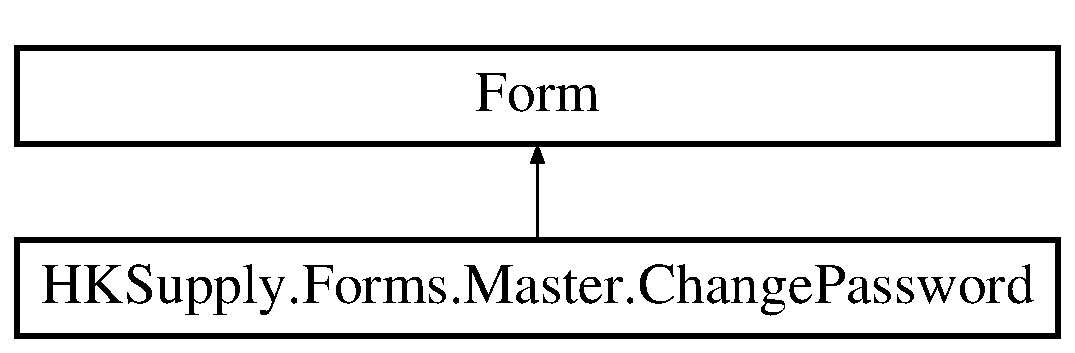
\includegraphics[height=2.000000cm]{class_h_k_supply_1_1_forms_1_1_master_1_1_change_password}
\end{center}
\end{figure}
\subsection*{Public Member Functions}
\begin{DoxyCompactItemize}
\item 
\mbox{\Hypertarget{class_h_k_supply_1_1_forms_1_1_master_1_1_change_password_aede98523b7abd2b8e57d2f7eb1f58154}\label{class_h_k_supply_1_1_forms_1_1_master_1_1_change_password_aede98523b7abd2b8e57d2f7eb1f58154}} 
{\bfseries Change\+Password} (\hyperlink{class_h_k_supply_1_1_models_1_1_user}{User} user)
\end{DoxyCompactItemize}
\subsection*{Protected Member Functions}
\begin{DoxyCompactItemize}
\item 
override void \hyperlink{class_h_k_supply_1_1_forms_1_1_master_1_1_change_password_a4370e4e0a208baadce764ed1081fb017}{Dispose} (bool disposing)
\begin{DoxyCompactList}\small\item\em Clean up any resources being used. \end{DoxyCompactList}\end{DoxyCompactItemize}


\subsection{Member Function Documentation}
\mbox{\Hypertarget{class_h_k_supply_1_1_forms_1_1_master_1_1_change_password_a4370e4e0a208baadce764ed1081fb017}\label{class_h_k_supply_1_1_forms_1_1_master_1_1_change_password_a4370e4e0a208baadce764ed1081fb017}} 
\index{H\+K\+Supply\+::\+Forms\+::\+Master\+::\+Change\+Password@{H\+K\+Supply\+::\+Forms\+::\+Master\+::\+Change\+Password}!Dispose@{Dispose}}
\index{Dispose@{Dispose}!H\+K\+Supply\+::\+Forms\+::\+Master\+::\+Change\+Password@{H\+K\+Supply\+::\+Forms\+::\+Master\+::\+Change\+Password}}
\subsubsection{\texorpdfstring{Dispose()}{Dispose()}}
{\footnotesize\ttfamily override void H\+K\+Supply.\+Forms.\+Master.\+Change\+Password.\+Dispose (\begin{DoxyParamCaption}\item[{bool}]{disposing }\end{DoxyParamCaption})\hspace{0.3cm}{\ttfamily [protected]}}



Clean up any resources being used. 


\begin{DoxyParams}{Parameters}
{\em disposing} & true if managed resources should be disposed; otherwise, false.\\
\hline
\end{DoxyParams}


The documentation for this class was generated from the following files\+:\begin{DoxyCompactItemize}
\item 
H\+K\+Supply/\+Forms/\+Master/Change\+Password.\+cs\item 
H\+K\+Supply/\+Forms/\+Master/Change\+Password.\+Designer.\+cs\end{DoxyCompactItemize}

\hypertarget{class_h_k_supply_1_1_models_1_1_customer}{}\section{H\+K\+Supply.\+Models.\+Customer Class Reference}
\label{class_h_k_supply_1_1_models_1_1_customer}\index{H\+K\+Supply.\+Models.\+Customer@{H\+K\+Supply.\+Models.\+Customer}}
\subsection*{Public Member Functions}
\begin{DoxyCompactItemize}
\item 
\mbox{\Hypertarget{class_h_k_supply_1_1_models_1_1_customer_a7e21d342fe37d5133dbaff9c32f35d05}\label{class_h_k_supply_1_1_models_1_1_customer_a7e21d342fe37d5133dbaff9c32f35d05}} 
override bool {\bfseries Equals} (object obj)
\item 
\mbox{\Hypertarget{class_h_k_supply_1_1_models_1_1_customer_a1277096021a0d574871c50508c576f85}\label{class_h_k_supply_1_1_models_1_1_customer_a1277096021a0d574871c50508c576f85}} 
override int {\bfseries Get\+Hash\+Code} ()
\end{DoxyCompactItemize}
\subsection*{Properties}
\begin{DoxyCompactItemize}
\item 
\mbox{\Hypertarget{class_h_k_supply_1_1_models_1_1_customer_ac4578adc9b1a3705f8169db9a7108757}\label{class_h_k_supply_1_1_models_1_1_customer_ac4578adc9b1a3705f8169db9a7108757}} 
int {\bfseries id\+Ver}\hspace{0.3cm}{\ttfamily  \mbox{[}get, set\mbox{]}}
\item 
\mbox{\Hypertarget{class_h_k_supply_1_1_models_1_1_customer_ad2c25c0c06f546f59d4d0036ef1f08c2}\label{class_h_k_supply_1_1_models_1_1_customer_ad2c25c0c06f546f59d4d0036ef1f08c2}} 
int {\bfseries id\+Sub\+Ver}\hspace{0.3cm}{\ttfamily  \mbox{[}get, set\mbox{]}}
\item 
\mbox{\Hypertarget{class_h_k_supply_1_1_models_1_1_customer_a22afbd1b11b69d47b922a08f29ac8ac7}\label{class_h_k_supply_1_1_models_1_1_customer_a22afbd1b11b69d47b922a08f29ac8ac7}} 
Date\+Time {\bfseries Timestamp}\hspace{0.3cm}{\ttfamily  \mbox{[}get, set\mbox{]}}
\item 
\mbox{\Hypertarget{class_h_k_supply_1_1_models_1_1_customer_a51edcd11d975455737e96f741fdadf54}\label{class_h_k_supply_1_1_models_1_1_customer_a51edcd11d975455737e96f741fdadf54}} 
string {\bfseries id\+Customer}\hspace{0.3cm}{\ttfamily  \mbox{[}get, set\mbox{]}}
\item 
\mbox{\Hypertarget{class_h_k_supply_1_1_models_1_1_customer_afccd2194383fd74d9c0056cd1aeff041}\label{class_h_k_supply_1_1_models_1_1_customer_afccd2194383fd74d9c0056cd1aeff041}} 
string {\bfseries Cust\+Name}\hspace{0.3cm}{\ttfamily  \mbox{[}get, set\mbox{]}}
\item 
\mbox{\Hypertarget{class_h_k_supply_1_1_models_1_1_customer_ac107c439966d40fbb00176e09e4682b5}\label{class_h_k_supply_1_1_models_1_1_customer_ac107c439966d40fbb00176e09e4682b5}} 
bool {\bfseries Active}\hspace{0.3cm}{\ttfamily  \mbox{[}get, set\mbox{]}}
\item 
\mbox{\Hypertarget{class_h_k_supply_1_1_models_1_1_customer_aaaadc5018a79479be7d43fad413dc3b0}\label{class_h_k_supply_1_1_models_1_1_customer_aaaadc5018a79479be7d43fad413dc3b0}} 
string {\bfseries V\+A\+T\+Num}\hspace{0.3cm}{\ttfamily  \mbox{[}get, set\mbox{]}}
\item 
\mbox{\Hypertarget{class_h_k_supply_1_1_models_1_1_customer_aa96f375cec2cf3a749f72525b1ce4f36}\label{class_h_k_supply_1_1_models_1_1_customer_aa96f375cec2cf3a749f72525b1ce4f36}} 
string {\bfseries Shiping\+Address}\hspace{0.3cm}{\ttfamily  \mbox{[}get, set\mbox{]}}
\item 
\mbox{\Hypertarget{class_h_k_supply_1_1_models_1_1_customer_a0ef5a3d143c02f5f01034f63616ec88b}\label{class_h_k_supply_1_1_models_1_1_customer_a0ef5a3d143c02f5f01034f63616ec88b}} 
string {\bfseries Billing\+Address}\hspace{0.3cm}{\ttfamily  \mbox{[}get, set\mbox{]}}
\item 
\mbox{\Hypertarget{class_h_k_supply_1_1_models_1_1_customer_a52ec06dbf5626f8fd7b46bd0189fc0f5}\label{class_h_k_supply_1_1_models_1_1_customer_a52ec06dbf5626f8fd7b46bd0189fc0f5}} 
string {\bfseries Contact\+Name}\hspace{0.3cm}{\ttfamily  \mbox{[}get, set\mbox{]}}
\item 
\mbox{\Hypertarget{class_h_k_supply_1_1_models_1_1_customer_a575063986e551c006263f89b4ab6b522}\label{class_h_k_supply_1_1_models_1_1_customer_a575063986e551c006263f89b4ab6b522}} 
string {\bfseries Contact\+Phone}\hspace{0.3cm}{\ttfamily  \mbox{[}get, set\mbox{]}}
\item 
\mbox{\Hypertarget{class_h_k_supply_1_1_models_1_1_customer_aafc92abc1367162a2cfd9aafeeff3bcd}\label{class_h_k_supply_1_1_models_1_1_customer_aafc92abc1367162a2cfd9aafeeff3bcd}} 
int {\bfseries id\+Incoterm}\hspace{0.3cm}{\ttfamily  \mbox{[}get, set\mbox{]}}
\item 
\mbox{\Hypertarget{class_h_k_supply_1_1_models_1_1_customer_a63268d32fbf9d3e7ed3ad42b52e0ed3d}\label{class_h_k_supply_1_1_models_1_1_customer_a63268d32fbf9d3e7ed3ad42b52e0ed3d}} 
int {\bfseries id\+Payment\+Terms}\hspace{0.3cm}{\ttfamily  \mbox{[}get, set\mbox{]}}
\item 
\mbox{\Hypertarget{class_h_k_supply_1_1_models_1_1_customer_a60662a4e763416385919b83cfc18cadd}\label{class_h_k_supply_1_1_models_1_1_customer_a60662a4e763416385919b83cfc18cadd}} 
string {\bfseries Currency}\hspace{0.3cm}{\ttfamily  \mbox{[}get, set\mbox{]}}
\end{DoxyCompactItemize}


The documentation for this class was generated from the following file\+:\begin{DoxyCompactItemize}
\item 
H\+K\+Supply/\+Models/Customer.\+cs\end{DoxyCompactItemize}

\hypertarget{class_h_k_supply_1_1_migrations_1_1_customer}{}\section{H\+K\+Supply.\+Migrations.\+Customer Class Reference}
\label{class_h_k_supply_1_1_migrations_1_1_customer}\index{H\+K\+Supply.\+Migrations.\+Customer@{H\+K\+Supply.\+Migrations.\+Customer}}
Inheritance diagram for H\+K\+Supply.\+Migrations.\+Customer\+:\begin{figure}[H]
\begin{center}
\leavevmode
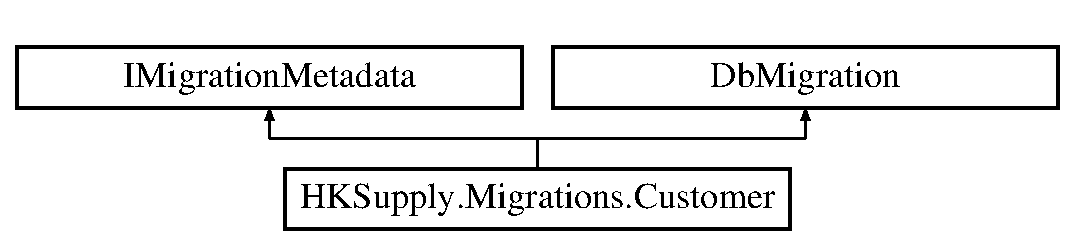
\includegraphics[height=2.000000cm]{class_h_k_supply_1_1_migrations_1_1_customer}
\end{center}
\end{figure}
\subsection*{Public Member Functions}
\begin{DoxyCompactItemize}
\item 
\mbox{\Hypertarget{class_h_k_supply_1_1_migrations_1_1_customer_a9d32a655fbb798821b0d9991eadd4a2f}\label{class_h_k_supply_1_1_migrations_1_1_customer_a9d32a655fbb798821b0d9991eadd4a2f}} 
override void {\bfseries Up} ()
\item 
\mbox{\Hypertarget{class_h_k_supply_1_1_migrations_1_1_customer_acc6e78c39b5f866e1b4dfec67ddd5c35}\label{class_h_k_supply_1_1_migrations_1_1_customer_acc6e78c39b5f866e1b4dfec67ddd5c35}} 
override void {\bfseries Down} ()
\end{DoxyCompactItemize}


The documentation for this class was generated from the following files\+:\begin{DoxyCompactItemize}
\item 
H\+K\+Supply/\+Migrations/201703081042226\+\_\+\+Customer.\+cs\item 
H\+K\+Supply/\+Migrations/201703081042226\+\_\+\+Customer.\+Designer.\+cs\end{DoxyCompactItemize}

\hypertarget{class_h_k_supply_1_1_models_1_1_customer_history}{}\section{H\+K\+Supply.\+Models.\+Customer\+History Class Reference}
\label{class_h_k_supply_1_1_models_1_1_customer_history}\index{H\+K\+Supply.\+Models.\+Customer\+History@{H\+K\+Supply.\+Models.\+Customer\+History}}
\subsection*{Public Member Functions}
\begin{DoxyCompactItemize}
\item 
\mbox{\Hypertarget{class_h_k_supply_1_1_models_1_1_customer_history_a7b1d5ad2746e1733fecebb4744187e22}\label{class_h_k_supply_1_1_models_1_1_customer_history_a7b1d5ad2746e1733fecebb4744187e22}} 
override bool {\bfseries Equals} (object obj)
\item 
\mbox{\Hypertarget{class_h_k_supply_1_1_models_1_1_customer_history_a9ce1510ea0fc18dfb2797f758fbcb88e}\label{class_h_k_supply_1_1_models_1_1_customer_history_a9ce1510ea0fc18dfb2797f758fbcb88e}} 
override int {\bfseries Get\+Hash\+Code} ()
\end{DoxyCompactItemize}
\subsection*{Static Public Member Functions}
\begin{DoxyCompactItemize}
\item 
\mbox{\Hypertarget{class_h_k_supply_1_1_models_1_1_customer_history_a1d54538a20700d9fd1b68cf979830fad}\label{class_h_k_supply_1_1_models_1_1_customer_history_a1d54538a20700d9fd1b68cf979830fad}} 
static implicit {\bfseries operator Customer\+History} (\mbox{\hyperlink{class_h_k_supply_1_1_models_1_1_customer}{Customer}} c)
\end{DoxyCompactItemize}
\subsection*{Properties}
\begin{DoxyCompactItemize}
\item 
\mbox{\Hypertarget{class_h_k_supply_1_1_models_1_1_customer_history_adc9862f74bd7e4097520ab8e42162f52}\label{class_h_k_supply_1_1_models_1_1_customer_history_adc9862f74bd7e4097520ab8e42162f52}} 
int {\bfseries Id\+Ver}\hspace{0.3cm}{\ttfamily  \mbox{[}get, set\mbox{]}}
\item 
\mbox{\Hypertarget{class_h_k_supply_1_1_models_1_1_customer_history_a6c531db8c25e1d19fef8d57f448f2c89}\label{class_h_k_supply_1_1_models_1_1_customer_history_a6c531db8c25e1d19fef8d57f448f2c89}} 
int {\bfseries Id\+Sub\+Ver}\hspace{0.3cm}{\ttfamily  \mbox{[}get, set\mbox{]}}
\item 
\mbox{\Hypertarget{class_h_k_supply_1_1_models_1_1_customer_history_a58e5e7fcc5efb1ae4b1883870e766007}\label{class_h_k_supply_1_1_models_1_1_customer_history_a58e5e7fcc5efb1ae4b1883870e766007}} 
Date\+Time {\bfseries Timestamp}\hspace{0.3cm}{\ttfamily  \mbox{[}get, set\mbox{]}}
\item 
\mbox{\Hypertarget{class_h_k_supply_1_1_models_1_1_customer_history_a21cc5c584c03af881a9cbc0f96ca1657}\label{class_h_k_supply_1_1_models_1_1_customer_history_a21cc5c584c03af881a9cbc0f96ca1657}} 
string {\bfseries Id\+Customer}\hspace{0.3cm}{\ttfamily  \mbox{[}get, set\mbox{]}}
\item 
\mbox{\Hypertarget{class_h_k_supply_1_1_models_1_1_customer_history_a4663303feccbc075102ab520044522e3}\label{class_h_k_supply_1_1_models_1_1_customer_history_a4663303feccbc075102ab520044522e3}} 
string {\bfseries Customer\+Name}\hspace{0.3cm}{\ttfamily  \mbox{[}get, set\mbox{]}}
\item 
\mbox{\Hypertarget{class_h_k_supply_1_1_models_1_1_customer_history_aca19f538f063b504473ea5405c90786e}\label{class_h_k_supply_1_1_models_1_1_customer_history_aca19f538f063b504473ea5405c90786e}} 
bool {\bfseries Active}\hspace{0.3cm}{\ttfamily  \mbox{[}get, set\mbox{]}}
\item 
\mbox{\Hypertarget{class_h_k_supply_1_1_models_1_1_customer_history_a800f04c7eb0959c9c47028c47a3f18c5}\label{class_h_k_supply_1_1_models_1_1_customer_history_a800f04c7eb0959c9c47028c47a3f18c5}} 
string {\bfseries V\+A\+T\+Num}\hspace{0.3cm}{\ttfamily  \mbox{[}get, set\mbox{]}}
\item 
\mbox{\Hypertarget{class_h_k_supply_1_1_models_1_1_customer_history_a3ea941a1239344f09b77ed4bc7ecd972}\label{class_h_k_supply_1_1_models_1_1_customer_history_a3ea941a1239344f09b77ed4bc7ecd972}} 
string {\bfseries Shipping\+Address}\hspace{0.3cm}{\ttfamily  \mbox{[}get, set\mbox{]}}
\item 
\mbox{\Hypertarget{class_h_k_supply_1_1_models_1_1_customer_history_a39aef49c4b0abb006b4fef47b042f640}\label{class_h_k_supply_1_1_models_1_1_customer_history_a39aef49c4b0abb006b4fef47b042f640}} 
string {\bfseries Shipping\+Address2}\hspace{0.3cm}{\ttfamily  \mbox{[}get, set\mbox{]}}
\item 
\mbox{\Hypertarget{class_h_k_supply_1_1_models_1_1_customer_history_a83fc36dccad98cd673cf923b8f81ca2d}\label{class_h_k_supply_1_1_models_1_1_customer_history_a83fc36dccad98cd673cf923b8f81ca2d}} 
string {\bfseries Shipping\+Address\+Zh}\hspace{0.3cm}{\ttfamily  \mbox{[}get, set\mbox{]}}
\item 
\mbox{\Hypertarget{class_h_k_supply_1_1_models_1_1_customer_history_a29eee64eacce6301a645a19df2580fd7}\label{class_h_k_supply_1_1_models_1_1_customer_history_a29eee64eacce6301a645a19df2580fd7}} 
string {\bfseries Shipping\+Address\+Zh2}\hspace{0.3cm}{\ttfamily  \mbox{[}get, set\mbox{]}}
\item 
\mbox{\Hypertarget{class_h_k_supply_1_1_models_1_1_customer_history_a8c60f8d3185afeb8764d61bde61b89bb}\label{class_h_k_supply_1_1_models_1_1_customer_history_a8c60f8d3185afeb8764d61bde61b89bb}} 
string {\bfseries Billing\+Address}\hspace{0.3cm}{\ttfamily  \mbox{[}get, set\mbox{]}}
\item 
\mbox{\Hypertarget{class_h_k_supply_1_1_models_1_1_customer_history_a4769ca2bdb8cd8567b12191ccdd1aea8}\label{class_h_k_supply_1_1_models_1_1_customer_history_a4769ca2bdb8cd8567b12191ccdd1aea8}} 
string {\bfseries Billing\+Address2}\hspace{0.3cm}{\ttfamily  \mbox{[}get, set\mbox{]}}
\item 
\mbox{\Hypertarget{class_h_k_supply_1_1_models_1_1_customer_history_aca2b155d9bb3cbd22d3fda1376205998}\label{class_h_k_supply_1_1_models_1_1_customer_history_aca2b155d9bb3cbd22d3fda1376205998}} 
string {\bfseries Billing\+Address\+Zh}\hspace{0.3cm}{\ttfamily  \mbox{[}get, set\mbox{]}}
\item 
\mbox{\Hypertarget{class_h_k_supply_1_1_models_1_1_customer_history_ab48a594b73d50080f31e5e26d238ab7b}\label{class_h_k_supply_1_1_models_1_1_customer_history_ab48a594b73d50080f31e5e26d238ab7b}} 
string {\bfseries Billing\+Address\+Zh2}\hspace{0.3cm}{\ttfamily  \mbox{[}get, set\mbox{]}}
\item 
\mbox{\Hypertarget{class_h_k_supply_1_1_models_1_1_customer_history_a66da89d7a3551f633f2e746a7f65191e}\label{class_h_k_supply_1_1_models_1_1_customer_history_a66da89d7a3551f633f2e746a7f65191e}} 
string {\bfseries Contact\+Name}\hspace{0.3cm}{\ttfamily  \mbox{[}get, set\mbox{]}}
\item 
\mbox{\Hypertarget{class_h_k_supply_1_1_models_1_1_customer_history_a61ee6495b3a29d9db714d87655951eb7}\label{class_h_k_supply_1_1_models_1_1_customer_history_a61ee6495b3a29d9db714d87655951eb7}} 
string {\bfseries Contact\+Name\+Zh}\hspace{0.3cm}{\ttfamily  \mbox{[}get, set\mbox{]}}
\item 
\mbox{\Hypertarget{class_h_k_supply_1_1_models_1_1_customer_history_a5f2166fba0c1b036b6575c82f87663f2}\label{class_h_k_supply_1_1_models_1_1_customer_history_a5f2166fba0c1b036b6575c82f87663f2}} 
string {\bfseries Contact\+Phone}\hspace{0.3cm}{\ttfamily  \mbox{[}get, set\mbox{]}}
\item 
\mbox{\Hypertarget{class_h_k_supply_1_1_models_1_1_customer_history_aec0e11a42b3589f8b354b5d12684e32a}\label{class_h_k_supply_1_1_models_1_1_customer_history_aec0e11a42b3589f8b354b5d12684e32a}} 
string {\bfseries Comments}\hspace{0.3cm}{\ttfamily  \mbox{[}get, set\mbox{]}}
\item 
\mbox{\Hypertarget{class_h_k_supply_1_1_models_1_1_customer_history_a2882c7f38df30fa9cf49ffb1f43f4d68}\label{class_h_k_supply_1_1_models_1_1_customer_history_a2882c7f38df30fa9cf49ffb1f43f4d68}} 
string {\bfseries Id\+Incoterm}\hspace{0.3cm}{\ttfamily  \mbox{[}get, set\mbox{]}}
\item 
\mbox{\Hypertarget{class_h_k_supply_1_1_models_1_1_customer_history_ae05f292e965cb9e5d835bafa9393ade8}\label{class_h_k_supply_1_1_models_1_1_customer_history_ae05f292e965cb9e5d835bafa9393ade8}} 
string {\bfseries Id\+Payment\+Terms}\hspace{0.3cm}{\ttfamily  \mbox{[}get, set\mbox{]}}
\item 
\mbox{\Hypertarget{class_h_k_supply_1_1_models_1_1_customer_history_acbc65c2d2e5027752fd91dfc1ec82036}\label{class_h_k_supply_1_1_models_1_1_customer_history_acbc65c2d2e5027752fd91dfc1ec82036}} 
string {\bfseries Id\+Default\+Currency}\hspace{0.3cm}{\ttfamily  \mbox{[}get, set\mbox{]}}
\item 
\mbox{\Hypertarget{class_h_k_supply_1_1_models_1_1_customer_history_a83245fa9151559f396ed7c8bd59f4ca5}\label{class_h_k_supply_1_1_models_1_1_customer_history_a83245fa9151559f396ed7c8bd59f4ca5}} 
bool {\bfseries Factory}\hspace{0.3cm}{\ttfamily  \mbox{[}get, set\mbox{]}}
\item 
\mbox{\Hypertarget{class_h_k_supply_1_1_models_1_1_customer_history_ae897dd3975eb0a3766e4e9ac6e2c673c}\label{class_h_k_supply_1_1_models_1_1_customer_history_ae897dd3975eb0a3766e4e9ac6e2c673c}} 
string {\bfseries User}\hspace{0.3cm}{\ttfamily  \mbox{[}get, set\mbox{]}}
\end{DoxyCompactItemize}


The documentation for this class was generated from the following file\+:\begin{DoxyCompactItemize}
\item 
H\+K\+Supply/\+Models/Customer\+History.\+cs\end{DoxyCompactItemize}

\hypertarget{class_custom_controls_1_1_custom_tool_strip_menu_item}{}\section{Custom\+Controls.\+Custom\+Tool\+Strip\+Menu\+Item Class Reference}
\label{class_custom_controls_1_1_custom_tool_strip_menu_item}\index{Custom\+Controls.\+Custom\+Tool\+Strip\+Menu\+Item@{Custom\+Controls.\+Custom\+Tool\+Strip\+Menu\+Item}}
Inheritance diagram for Custom\+Controls.\+Custom\+Tool\+Strip\+Menu\+Item\+:\begin{figure}[H]
\begin{center}
\leavevmode
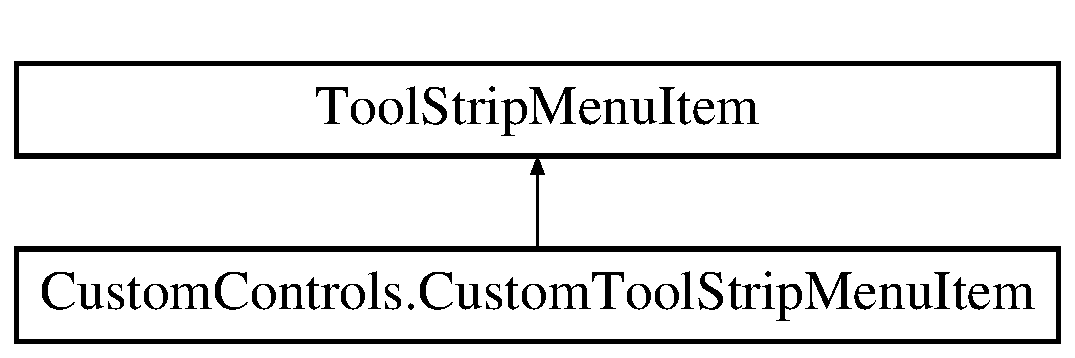
\includegraphics[height=2.000000cm]{class_custom_controls_1_1_custom_tool_strip_menu_item}
\end{center}
\end{figure}
\subsection*{Public Member Functions}
\begin{DoxyCompactItemize}
\item 
\mbox{\Hypertarget{class_custom_controls_1_1_custom_tool_strip_menu_item_a3b07c5d51a0a1b0d2c1bfa23489e0454}\label{class_custom_controls_1_1_custom_tool_strip_menu_item_a3b07c5d51a0a1b0d2c1bfa23489e0454}} 
{\bfseries Custom\+Tool\+Strip\+Menu\+Item} (string text, Image image, Event\+Handler on\+Click, string name)
\end{DoxyCompactItemize}
\subsection*{Protected Member Functions}
\begin{DoxyCompactItemize}
\item 
override void \hyperlink{class_custom_controls_1_1_custom_tool_strip_menu_item_a09da84511dccda9f78441c82ff2f4508}{Dispose} (bool disposing)
\begin{DoxyCompactList}\small\item\em Limpiar los recursos que se estén utilizando. \end{DoxyCompactList}\end{DoxyCompactItemize}
\subsection*{Properties}
\begin{DoxyCompactItemize}
\item 
\mbox{\Hypertarget{class_custom_controls_1_1_custom_tool_strip_menu_item_a2533ed0f2c4c4b248b1abc49e716c2a6}\label{class_custom_controls_1_1_custom_tool_strip_menu_item_a2533ed0f2c4c4b248b1abc49e716c2a6}} 
string {\bfseries Form\+Name}\hspace{0.3cm}{\ttfamily  \mbox{[}get, set\mbox{]}}
\end{DoxyCompactItemize}


\subsection{Member Function Documentation}
\mbox{\Hypertarget{class_custom_controls_1_1_custom_tool_strip_menu_item_a09da84511dccda9f78441c82ff2f4508}\label{class_custom_controls_1_1_custom_tool_strip_menu_item_a09da84511dccda9f78441c82ff2f4508}} 
\index{Custom\+Controls\+::\+Custom\+Tool\+Strip\+Menu\+Item@{Custom\+Controls\+::\+Custom\+Tool\+Strip\+Menu\+Item}!Dispose@{Dispose}}
\index{Dispose@{Dispose}!Custom\+Controls\+::\+Custom\+Tool\+Strip\+Menu\+Item@{Custom\+Controls\+::\+Custom\+Tool\+Strip\+Menu\+Item}}
\subsubsection{\texorpdfstring{Dispose()}{Dispose()}}
{\footnotesize\ttfamily override void Custom\+Controls.\+Custom\+Tool\+Strip\+Menu\+Item.\+Dispose (\begin{DoxyParamCaption}\item[{bool}]{disposing }\end{DoxyParamCaption})\hspace{0.3cm}{\ttfamily [protected]}}



Limpiar los recursos que se estén utilizando. 


\begin{DoxyParams}{Parameters}
{\em disposing} & true si los recursos administrados se deben eliminar; false en caso contrario.\\
\hline
\end{DoxyParams}


The documentation for this class was generated from the following files\+:\begin{DoxyCompactItemize}
\item 
Custom\+Controls/Custom\+Tool\+Strip\+Menu\+Item.\+cs\item 
Custom\+Controls/Custom\+Tool\+Strip\+Menu\+Item.\+Designer.\+cs\end{DoxyCompactItemize}

\hypertarget{class_h_k_supply_1_1_services_1_1_implementations_1_1_e_f_customer}{}\section{H\+K\+Supply.\+Services.\+Implementations.\+E\+F\+Customer Class Reference}
\label{class_h_k_supply_1_1_services_1_1_implementations_1_1_e_f_customer}\index{H\+K\+Supply.\+Services.\+Implementations.\+E\+F\+Customer@{H\+K\+Supply.\+Services.\+Implementations.\+E\+F\+Customer}}
Inheritance diagram for H\+K\+Supply.\+Services.\+Implementations.\+E\+F\+Customer\+:\begin{figure}[H]
\begin{center}
\leavevmode
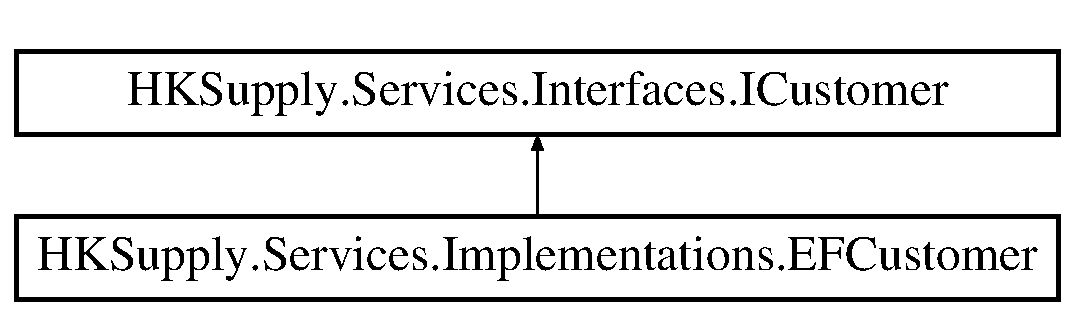
\includegraphics[height=2.000000cm]{class_h_k_supply_1_1_services_1_1_implementations_1_1_e_f_customer}
\end{center}
\end{figure}
\subsection*{Public Member Functions}
\begin{DoxyCompactItemize}
\item 
\mbox{\Hypertarget{class_h_k_supply_1_1_services_1_1_implementations_1_1_e_f_customer_a8caba8c3706d212709d73ff4e2e94e1e}\label{class_h_k_supply_1_1_services_1_1_implementations_1_1_e_f_customer_a8caba8c3706d212709d73ff4e2e94e1e}} 
bool {\bfseries New\+Customer} (\hyperlink{class_h_k_supply_1_1_models_1_1_customer}{Customer} new\+Customer)
\item 
\mbox{\Hypertarget{class_h_k_supply_1_1_services_1_1_implementations_1_1_e_f_customer_af7bd47be2eff71310dd5ad5e4157bfa4}\label{class_h_k_supply_1_1_services_1_1_implementations_1_1_e_f_customer_af7bd47be2eff71310dd5ad5e4157bfa4}} 
bool {\bfseries Update\+Customer} (\hyperlink{class_h_k_supply_1_1_models_1_1_customer}{Customer} update\+Customer, bool new\+Ver=false)
\item 
\mbox{\Hypertarget{class_h_k_supply_1_1_services_1_1_implementations_1_1_e_f_customer_a88c703ed6108d30abbed42876d524fb3}\label{class_h_k_supply_1_1_services_1_1_implementations_1_1_e_f_customer_a88c703ed6108d30abbed42876d524fb3}} 
\hyperlink{class_h_k_supply_1_1_models_1_1_customer}{Customer} {\bfseries Get\+Customer\+By\+Id} (string id\+Customer)
\item 
\mbox{\Hypertarget{class_h_k_supply_1_1_services_1_1_implementations_1_1_e_f_customer_a2688e050817d243a2c424293b2922005}\label{class_h_k_supply_1_1_services_1_1_implementations_1_1_e_f_customer_a2688e050817d243a2c424293b2922005}} 
List$<$ \hyperlink{class_h_k_supply_1_1_models_1_1_customer}{Customer} $>$ {\bfseries Get\+Customers} ()
\end{DoxyCompactItemize}


The documentation for this class was generated from the following file\+:\begin{DoxyCompactItemize}
\item 
H\+K\+Supply/\+Services/\+Implementations/E\+F\+Customer.\+cs\end{DoxyCompactItemize}

\hypertarget{class_h_k_supply_1_1_services_1_1_implementations_1_1_e_f_functionality}{}\section{H\+K\+Supply.\+Services.\+Implementations.\+E\+F\+Functionality Class Reference}
\label{class_h_k_supply_1_1_services_1_1_implementations_1_1_e_f_functionality}\index{H\+K\+Supply.\+Services.\+Implementations.\+E\+F\+Functionality@{H\+K\+Supply.\+Services.\+Implementations.\+E\+F\+Functionality}}


Controlador Entity Framework para Functionality  


Inheritance diagram for H\+K\+Supply.\+Services.\+Implementations.\+E\+F\+Functionality\+:\begin{figure}[H]
\begin{center}
\leavevmode
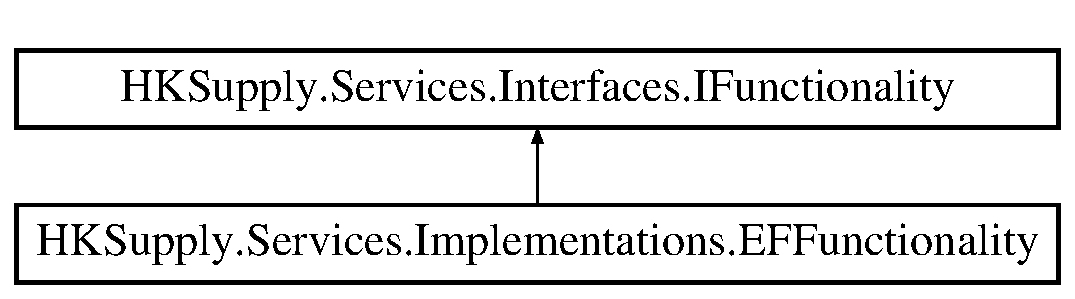
\includegraphics[height=2.000000cm]{class_h_k_supply_1_1_services_1_1_implementations_1_1_e_f_functionality}
\end{center}
\end{figure}
\subsection*{Public Member Functions}
\begin{DoxyCompactItemize}
\item 
I\+Enumerable$<$ \mbox{\hyperlink{class_h_k_supply_1_1_models_1_1_functionality}{Functionality}} $>$ \mbox{\hyperlink{class_h_k_supply_1_1_services_1_1_implementations_1_1_e_f_functionality_ab92f666d01076cffafbddbb91c5cf6af}{Get\+All\+Functionalities}} ()
\begin{DoxyCompactList}\small\item\em Obtener todas las funcionalidades de la base de datos \end{DoxyCompactList}\item 
\mbox{\hyperlink{class_h_k_supply_1_1_models_1_1_functionality}{Functionality}} \mbox{\hyperlink{class_h_k_supply_1_1_services_1_1_implementations_1_1_e_f_functionality_a0aa6fc75b8f1ddf6532f39a84bc50ad9}{Get\+Functionality\+By\+Id}} (int functionality\+Id)
\begin{DoxyCompactList}\small\item\em Obtener una funcionalidad a través de un Id \end{DoxyCompactList}\item 
\mbox{\hyperlink{class_h_k_supply_1_1_models_1_1_functionality}{Functionality}} \mbox{\hyperlink{class_h_k_supply_1_1_services_1_1_implementations_1_1_e_f_functionality_a655784ce048904e9f27a827ccf2a7a79}{Get\+Functionality\+By\+Name}} (string functionality\+Name)
\begin{DoxyCompactList}\small\item\em Obtener una funcionalidad por su nombre \end{DoxyCompactList}\item 
\mbox{\hyperlink{class_h_k_supply_1_1_models_1_1_functionality}{Functionality}} \mbox{\hyperlink{class_h_k_supply_1_1_services_1_1_implementations_1_1_e_f_functionality_a43852b181d280c78c7c00b9d11c6d6c4}{New\+Functionality}} (\mbox{\hyperlink{class_h_k_supply_1_1_models_1_1_functionality}{Functionality}} new\+Functionality)
\begin{DoxyCompactList}\small\item\em Dar de alta una funcionalidad \end{DoxyCompactList}\item 
\mbox{\hyperlink{class_h_k_supply_1_1_models_1_1_functionality}{Functionality}} \mbox{\hyperlink{class_h_k_supply_1_1_services_1_1_implementations_1_1_e_f_functionality_ae4f83037cd6ef526f55de1a2ba442cc6}{Modify\+Functionality}} (\mbox{\hyperlink{class_h_k_supply_1_1_models_1_1_functionality}{Functionality}} mod\+Functionality)
\begin{DoxyCompactList}\small\item\em Modificar una funcionalidad \end{DoxyCompactList}\item 
bool \mbox{\hyperlink{class_h_k_supply_1_1_services_1_1_implementations_1_1_e_f_functionality_a2093874e195260c8963796b45aeba022}{Update\+Functionalities}} (I\+Enumerable$<$ \mbox{\hyperlink{class_h_k_supply_1_1_models_1_1_functionality}{Functionality}} $>$ functionalities\+To\+Update)
\begin{DoxyCompactList}\small\item\em Modificar un enumerable de funcionalidades \end{DoxyCompactList}\end{DoxyCompactItemize}


\subsection{Detailed Description}
Controlador Entity Framework para Functionality 



\subsection{Member Function Documentation}
\mbox{\Hypertarget{class_h_k_supply_1_1_services_1_1_implementations_1_1_e_f_functionality_ab92f666d01076cffafbddbb91c5cf6af}\label{class_h_k_supply_1_1_services_1_1_implementations_1_1_e_f_functionality_ab92f666d01076cffafbddbb91c5cf6af}} 
\index{H\+K\+Supply\+::\+Services\+::\+Implementations\+::\+E\+F\+Functionality@{H\+K\+Supply\+::\+Services\+::\+Implementations\+::\+E\+F\+Functionality}!Get\+All\+Functionalities@{Get\+All\+Functionalities}}
\index{Get\+All\+Functionalities@{Get\+All\+Functionalities}!H\+K\+Supply\+::\+Services\+::\+Implementations\+::\+E\+F\+Functionality@{H\+K\+Supply\+::\+Services\+::\+Implementations\+::\+E\+F\+Functionality}}
\subsubsection{\texorpdfstring{Get\+All\+Functionalities()}{GetAllFunctionalities()}}
{\footnotesize\ttfamily I\+Enumerable$<$\mbox{\hyperlink{class_h_k_supply_1_1_models_1_1_functionality}{Functionality}}$>$ H\+K\+Supply.\+Services.\+Implementations.\+E\+F\+Functionality.\+Get\+All\+Functionalities (\begin{DoxyParamCaption}{ }\end{DoxyParamCaption})}



Obtener todas las funcionalidades de la base de datos 

\begin{DoxyReturn}{Returns}

\end{DoxyReturn}


Implements \mbox{\hyperlink{interface_h_k_supply_1_1_services_1_1_interfaces_1_1_i_functionality}{H\+K\+Supply.\+Services.\+Interfaces.\+I\+Functionality}}.

\mbox{\Hypertarget{class_h_k_supply_1_1_services_1_1_implementations_1_1_e_f_functionality_a0aa6fc75b8f1ddf6532f39a84bc50ad9}\label{class_h_k_supply_1_1_services_1_1_implementations_1_1_e_f_functionality_a0aa6fc75b8f1ddf6532f39a84bc50ad9}} 
\index{H\+K\+Supply\+::\+Services\+::\+Implementations\+::\+E\+F\+Functionality@{H\+K\+Supply\+::\+Services\+::\+Implementations\+::\+E\+F\+Functionality}!Get\+Functionality\+By\+Id@{Get\+Functionality\+By\+Id}}
\index{Get\+Functionality\+By\+Id@{Get\+Functionality\+By\+Id}!H\+K\+Supply\+::\+Services\+::\+Implementations\+::\+E\+F\+Functionality@{H\+K\+Supply\+::\+Services\+::\+Implementations\+::\+E\+F\+Functionality}}
\subsubsection{\texorpdfstring{Get\+Functionality\+By\+Id()}{GetFunctionalityById()}}
{\footnotesize\ttfamily \mbox{\hyperlink{class_h_k_supply_1_1_models_1_1_functionality}{Functionality}} H\+K\+Supply.\+Services.\+Implementations.\+E\+F\+Functionality.\+Get\+Functionality\+By\+Id (\begin{DoxyParamCaption}\item[{int}]{functionality\+Id }\end{DoxyParamCaption})}



Obtener una funcionalidad a través de un Id 


\begin{DoxyParams}{Parameters}
{\em functionality\+Id} & \\
\hline
\end{DoxyParams}
\begin{DoxyReturn}{Returns}

\end{DoxyReturn}


Implements \mbox{\hyperlink{interface_h_k_supply_1_1_services_1_1_interfaces_1_1_i_functionality}{H\+K\+Supply.\+Services.\+Interfaces.\+I\+Functionality}}.

\mbox{\Hypertarget{class_h_k_supply_1_1_services_1_1_implementations_1_1_e_f_functionality_a655784ce048904e9f27a827ccf2a7a79}\label{class_h_k_supply_1_1_services_1_1_implementations_1_1_e_f_functionality_a655784ce048904e9f27a827ccf2a7a79}} 
\index{H\+K\+Supply\+::\+Services\+::\+Implementations\+::\+E\+F\+Functionality@{H\+K\+Supply\+::\+Services\+::\+Implementations\+::\+E\+F\+Functionality}!Get\+Functionality\+By\+Name@{Get\+Functionality\+By\+Name}}
\index{Get\+Functionality\+By\+Name@{Get\+Functionality\+By\+Name}!H\+K\+Supply\+::\+Services\+::\+Implementations\+::\+E\+F\+Functionality@{H\+K\+Supply\+::\+Services\+::\+Implementations\+::\+E\+F\+Functionality}}
\subsubsection{\texorpdfstring{Get\+Functionality\+By\+Name()}{GetFunctionalityByName()}}
{\footnotesize\ttfamily \mbox{\hyperlink{class_h_k_supply_1_1_models_1_1_functionality}{Functionality}} H\+K\+Supply.\+Services.\+Implementations.\+E\+F\+Functionality.\+Get\+Functionality\+By\+Name (\begin{DoxyParamCaption}\item[{string}]{functionality\+Name }\end{DoxyParamCaption})}



Obtener una funcionalidad por su nombre 


\begin{DoxyParams}{Parameters}
{\em functionality\+Name} & \\
\hline
\end{DoxyParams}
\begin{DoxyReturn}{Returns}

\end{DoxyReturn}


Implements \mbox{\hyperlink{interface_h_k_supply_1_1_services_1_1_interfaces_1_1_i_functionality}{H\+K\+Supply.\+Services.\+Interfaces.\+I\+Functionality}}.

\mbox{\Hypertarget{class_h_k_supply_1_1_services_1_1_implementations_1_1_e_f_functionality_ae4f83037cd6ef526f55de1a2ba442cc6}\label{class_h_k_supply_1_1_services_1_1_implementations_1_1_e_f_functionality_ae4f83037cd6ef526f55de1a2ba442cc6}} 
\index{H\+K\+Supply\+::\+Services\+::\+Implementations\+::\+E\+F\+Functionality@{H\+K\+Supply\+::\+Services\+::\+Implementations\+::\+E\+F\+Functionality}!Modify\+Functionality@{Modify\+Functionality}}
\index{Modify\+Functionality@{Modify\+Functionality}!H\+K\+Supply\+::\+Services\+::\+Implementations\+::\+E\+F\+Functionality@{H\+K\+Supply\+::\+Services\+::\+Implementations\+::\+E\+F\+Functionality}}
\subsubsection{\texorpdfstring{Modify\+Functionality()}{ModifyFunctionality()}}
{\footnotesize\ttfamily \mbox{\hyperlink{class_h_k_supply_1_1_models_1_1_functionality}{Functionality}} H\+K\+Supply.\+Services.\+Implementations.\+E\+F\+Functionality.\+Modify\+Functionality (\begin{DoxyParamCaption}\item[{\mbox{\hyperlink{class_h_k_supply_1_1_models_1_1_functionality}{Functionality}}}]{mod\+Functionality }\end{DoxyParamCaption})}



Modificar una funcionalidad 


\begin{DoxyParams}{Parameters}
{\em mod\+Functionality} & \\
\hline
\end{DoxyParams}
\begin{DoxyReturn}{Returns}
Objeto Functionality con la funcioliadad modificada
\end{DoxyReturn}


Modifica los campos\+:
\begin{DoxyItemize}
\item Category
\item Form\+Name 
\end{DoxyItemize}

Implements \mbox{\hyperlink{interface_h_k_supply_1_1_services_1_1_interfaces_1_1_i_functionality}{H\+K\+Supply.\+Services.\+Interfaces.\+I\+Functionality}}.

\mbox{\Hypertarget{class_h_k_supply_1_1_services_1_1_implementations_1_1_e_f_functionality_a43852b181d280c78c7c00b9d11c6d6c4}\label{class_h_k_supply_1_1_services_1_1_implementations_1_1_e_f_functionality_a43852b181d280c78c7c00b9d11c6d6c4}} 
\index{H\+K\+Supply\+::\+Services\+::\+Implementations\+::\+E\+F\+Functionality@{H\+K\+Supply\+::\+Services\+::\+Implementations\+::\+E\+F\+Functionality}!New\+Functionality@{New\+Functionality}}
\index{New\+Functionality@{New\+Functionality}!H\+K\+Supply\+::\+Services\+::\+Implementations\+::\+E\+F\+Functionality@{H\+K\+Supply\+::\+Services\+::\+Implementations\+::\+E\+F\+Functionality}}
\subsubsection{\texorpdfstring{New\+Functionality()}{NewFunctionality()}}
{\footnotesize\ttfamily \mbox{\hyperlink{class_h_k_supply_1_1_models_1_1_functionality}{Functionality}} H\+K\+Supply.\+Services.\+Implementations.\+E\+F\+Functionality.\+New\+Functionality (\begin{DoxyParamCaption}\item[{\mbox{\hyperlink{class_h_k_supply_1_1_models_1_1_functionality}{Functionality}}}]{new\+Functionality }\end{DoxyParamCaption})}



Dar de alta una funcionalidad 


\begin{DoxyParams}{Parameters}
{\em new\+Functionality} & \\
\hline
\end{DoxyParams}
\begin{DoxyReturn}{Returns}

\end{DoxyReturn}


Implements \mbox{\hyperlink{interface_h_k_supply_1_1_services_1_1_interfaces_1_1_i_functionality}{H\+K\+Supply.\+Services.\+Interfaces.\+I\+Functionality}}.

\mbox{\Hypertarget{class_h_k_supply_1_1_services_1_1_implementations_1_1_e_f_functionality_a2093874e195260c8963796b45aeba022}\label{class_h_k_supply_1_1_services_1_1_implementations_1_1_e_f_functionality_a2093874e195260c8963796b45aeba022}} 
\index{H\+K\+Supply\+::\+Services\+::\+Implementations\+::\+E\+F\+Functionality@{H\+K\+Supply\+::\+Services\+::\+Implementations\+::\+E\+F\+Functionality}!Update\+Functionalities@{Update\+Functionalities}}
\index{Update\+Functionalities@{Update\+Functionalities}!H\+K\+Supply\+::\+Services\+::\+Implementations\+::\+E\+F\+Functionality@{H\+K\+Supply\+::\+Services\+::\+Implementations\+::\+E\+F\+Functionality}}
\subsubsection{\texorpdfstring{Update\+Functionalities()}{UpdateFunctionalities()}}
{\footnotesize\ttfamily bool H\+K\+Supply.\+Services.\+Implementations.\+E\+F\+Functionality.\+Update\+Functionalities (\begin{DoxyParamCaption}\item[{I\+Enumerable$<$ \mbox{\hyperlink{class_h_k_supply_1_1_models_1_1_functionality}{Functionality}} $>$}]{functionalities\+To\+Update }\end{DoxyParamCaption})}



Modificar un enumerable de funcionalidades 


\begin{DoxyParams}{Parameters}
{\em functionalities\+To\+Update} & \\
\hline
\end{DoxyParams}
\begin{DoxyReturn}{Returns}
bool
\end{DoxyReturn}


Implements \mbox{\hyperlink{interface_h_k_supply_1_1_services_1_1_interfaces_1_1_i_functionality}{H\+K\+Supply.\+Services.\+Interfaces.\+I\+Functionality}}.



The documentation for this class was generated from the following file\+:\begin{DoxyCompactItemize}
\item 
H\+K\+Supply/\+Services/\+Implementations/E\+F\+Functionality.\+cs\end{DoxyCompactItemize}

\hypertarget{class_h_k_supply_1_1_services_1_1_implementations_1_1_e_f_functionality_role}{}\section{H\+K\+Supply.\+Services.\+Implementations.\+E\+F\+Functionality\+Role Class Reference}
\label{class_h_k_supply_1_1_services_1_1_implementations_1_1_e_f_functionality_role}\index{H\+K\+Supply.\+Services.\+Implementations.\+E\+F\+Functionality\+Role@{H\+K\+Supply.\+Services.\+Implementations.\+E\+F\+Functionality\+Role}}
Inheritance diagram for H\+K\+Supply.\+Services.\+Implementations.\+E\+F\+Functionality\+Role\+:\begin{figure}[H]
\begin{center}
\leavevmode
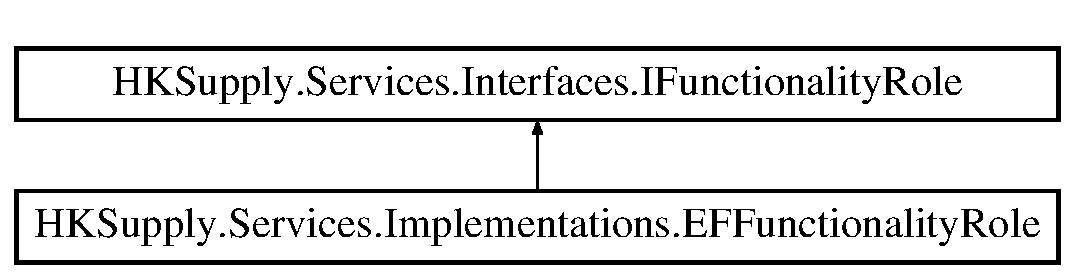
\includegraphics[height=2.000000cm]{class_h_k_supply_1_1_services_1_1_implementations_1_1_e_f_functionality_role}
\end{center}
\end{figure}
\subsection*{Public Member Functions}
\begin{DoxyCompactItemize}
\item 
\mbox{\Hypertarget{class_h_k_supply_1_1_services_1_1_implementations_1_1_e_f_functionality_role_a6c0fd4aad39788ef597f701f47032a85}\label{class_h_k_supply_1_1_services_1_1_implementations_1_1_e_f_functionality_role_a6c0fd4aad39788ef597f701f47032a85}} 
I\+Enumerable$<$ \hyperlink{class_h_k_supply_1_1_models_1_1_functionality_role}{Functionality\+Role} $>$ {\bfseries Get\+All\+Functionalities\+Role} ()
\item 
\mbox{\Hypertarget{class_h_k_supply_1_1_services_1_1_implementations_1_1_e_f_functionality_role_a1900a194c92ba75d17fe42830190895f}\label{class_h_k_supply_1_1_services_1_1_implementations_1_1_e_f_functionality_role_a1900a194c92ba75d17fe42830190895f}} 
\hyperlink{class_h_k_supply_1_1_models_1_1_functionality_role}{Functionality\+Role} {\bfseries Get\+Functionality\+Role} (int functionality\+Id, string role\+Id)
\item 
\mbox{\Hypertarget{class_h_k_supply_1_1_services_1_1_implementations_1_1_e_f_functionality_role_a0cec1ef9a2e1201cfffe604869e5192f}\label{class_h_k_supply_1_1_services_1_1_implementations_1_1_e_f_functionality_role_a0cec1ef9a2e1201cfffe604869e5192f}} 
I\+Enumerable$<$ \hyperlink{class_h_k_supply_1_1_models_1_1_functionality_role}{Functionality\+Role} $>$ {\bfseries Get\+Functionalities\+Role} (string role\+Id)
\item 
\mbox{\Hypertarget{class_h_k_supply_1_1_services_1_1_implementations_1_1_e_f_functionality_role_a1625ffb6313337132a446f831d357453}\label{class_h_k_supply_1_1_services_1_1_implementations_1_1_e_f_functionality_role_a1625ffb6313337132a446f831d357453}} 
I\+Enumerable$<$ string $>$ {\bfseries Get\+Functionalities\+Categories\+Role} (string role\+Id)
\item 
\mbox{\Hypertarget{class_h_k_supply_1_1_services_1_1_implementations_1_1_e_f_functionality_role_a07805a2c9809f3771b7ae34deb15b94b}\label{class_h_k_supply_1_1_services_1_1_implementations_1_1_e_f_functionality_role_a07805a2c9809f3771b7ae34deb15b94b}} 
\hyperlink{class_h_k_supply_1_1_models_1_1_functionality_role}{Functionality\+Role} {\bfseries New\+Functionality\+Role} (\hyperlink{class_h_k_supply_1_1_models_1_1_functionality_role}{Functionality\+Role} new\+Functionality\+Role)
\item 
\mbox{\Hypertarget{class_h_k_supply_1_1_services_1_1_implementations_1_1_e_f_functionality_role_a69bbb7f8593ea4e0e70ce96625cf80e4}\label{class_h_k_supply_1_1_services_1_1_implementations_1_1_e_f_functionality_role_a69bbb7f8593ea4e0e70ce96625cf80e4}} 
\hyperlink{class_h_k_supply_1_1_models_1_1_functionality_role}{Functionality\+Role} {\bfseries Modify\+Functionality\+Role} (\hyperlink{class_h_k_supply_1_1_models_1_1_functionality_role}{Functionality\+Role} mod\+Functionality\+Role)
\item 
\mbox{\Hypertarget{class_h_k_supply_1_1_services_1_1_implementations_1_1_e_f_functionality_role_a298798bba5c1a7e5a1db34803e3e4707}\label{class_h_k_supply_1_1_services_1_1_implementations_1_1_e_f_functionality_role_a298798bba5c1a7e5a1db34803e3e4707}} 
bool {\bfseries Update\+Functionalities\+Roles} (I\+Enumerable$<$ \hyperlink{class_h_k_supply_1_1_models_1_1_functionality_role}{Functionality\+Role} $>$ functionalities\+Roles\+To\+Update)
\end{DoxyCompactItemize}


The documentation for this class was generated from the following file\+:\begin{DoxyCompactItemize}
\item 
H\+K\+Supply/\+Services/\+Implementations/E\+F\+Functionality\+Role.\+cs\end{DoxyCompactItemize}

\hypertarget{class_h_k_supply_1_1_services_1_1_implementations_1_1_e_f_role}{}\section{H\+K\+Supply.\+Services.\+Implementations.\+E\+F\+Role Class Reference}
\label{class_h_k_supply_1_1_services_1_1_implementations_1_1_e_f_role}\index{H\+K\+Supply.\+Services.\+Implementations.\+E\+F\+Role@{H\+K\+Supply.\+Services.\+Implementations.\+E\+F\+Role}}


Controlador Entity Framework para Role  


Inheritance diagram for H\+K\+Supply.\+Services.\+Implementations.\+E\+F\+Role\+:\begin{figure}[H]
\begin{center}
\leavevmode
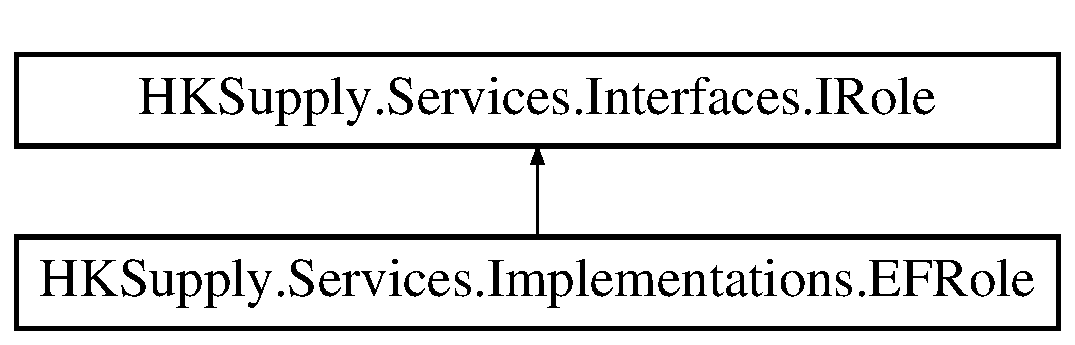
\includegraphics[height=2.000000cm]{class_h_k_supply_1_1_services_1_1_implementations_1_1_e_f_role}
\end{center}
\end{figure}
\subsection*{Public Member Functions}
\begin{DoxyCompactItemize}
\item 
I\+Enumerable$<$ \mbox{\hyperlink{class_h_k_supply_1_1_models_1_1_role}{Role}} $>$ \mbox{\hyperlink{class_h_k_supply_1_1_services_1_1_implementations_1_1_e_f_role_a7fd2f7f9bae498128f23ad0659e3ec4a}{Get\+Roles}} (bool all=true)
\begin{DoxyCompactList}\small\item\em Obtener la colección de roles del sistema. \end{DoxyCompactList}\item 
\mbox{\hyperlink{class_h_k_supply_1_1_models_1_1_role}{Role}} \mbox{\hyperlink{class_h_k_supply_1_1_services_1_1_implementations_1_1_e_f_role_ad4eb9194531a9215c4f1a20ab0d9aa54}{Get\+Role\+By\+Id}} (string role\+Id)
\begin{DoxyCompactList}\small\item\em Obtener un rol dado su Id \end{DoxyCompactList}\item 
\mbox{\hyperlink{class_h_k_supply_1_1_models_1_1_role}{Role}} \mbox{\hyperlink{class_h_k_supply_1_1_services_1_1_implementations_1_1_e_f_role_a549317ad8c8fb3353382a8cd36fa1b22}{New\+Role}} (\mbox{\hyperlink{class_h_k_supply_1_1_models_1_1_role}{Role}} new\+Role)
\begin{DoxyCompactList}\small\item\em Dar de alta un rol en el sistema \end{DoxyCompactList}\item 
bool \mbox{\hyperlink{class_h_k_supply_1_1_services_1_1_implementations_1_1_e_f_role_adf253e840ea77e23fd7c10899f316f21}{Disable\+Role}} (string role\+Id, string remarks)
\begin{DoxyCompactList}\small\item\em Deshabilitar un rol \end{DoxyCompactList}\item 
bool \mbox{\hyperlink{class_h_k_supply_1_1_services_1_1_implementations_1_1_e_f_role_a2d880fce95c33f7581f2e3310ca943ed}{Update\+Roles}} (I\+Enumerable$<$ \mbox{\hyperlink{class_h_k_supply_1_1_models_1_1_role}{Role}} $>$ roles\+To\+Update)
\begin{DoxyCompactList}\small\item\em Modificar una colección de roles \end{DoxyCompactList}\end{DoxyCompactItemize}


\subsection{Detailed Description}
Controlador Entity Framework para Role 



\subsection{Member Function Documentation}
\mbox{\Hypertarget{class_h_k_supply_1_1_services_1_1_implementations_1_1_e_f_role_adf253e840ea77e23fd7c10899f316f21}\label{class_h_k_supply_1_1_services_1_1_implementations_1_1_e_f_role_adf253e840ea77e23fd7c10899f316f21}} 
\index{H\+K\+Supply\+::\+Services\+::\+Implementations\+::\+E\+F\+Role@{H\+K\+Supply\+::\+Services\+::\+Implementations\+::\+E\+F\+Role}!Disable\+Role@{Disable\+Role}}
\index{Disable\+Role@{Disable\+Role}!H\+K\+Supply\+::\+Services\+::\+Implementations\+::\+E\+F\+Role@{H\+K\+Supply\+::\+Services\+::\+Implementations\+::\+E\+F\+Role}}
\subsubsection{\texorpdfstring{Disable\+Role()}{DisableRole()}}
{\footnotesize\ttfamily bool H\+K\+Supply.\+Services.\+Implementations.\+E\+F\+Role.\+Disable\+Role (\begin{DoxyParamCaption}\item[{string}]{role\+Id,  }\item[{string}]{remarks }\end{DoxyParamCaption})}



Deshabilitar un rol 


\begin{DoxyParams}{Parameters}
{\em role\+Id} & \\
\hline
{\em remarks} & \\
\hline
\end{DoxyParams}
\begin{DoxyReturn}{Returns}

\end{DoxyReturn}


Implements \mbox{\hyperlink{interface_h_k_supply_1_1_services_1_1_interfaces_1_1_i_role}{H\+K\+Supply.\+Services.\+Interfaces.\+I\+Role}}.

\mbox{\Hypertarget{class_h_k_supply_1_1_services_1_1_implementations_1_1_e_f_role_ad4eb9194531a9215c4f1a20ab0d9aa54}\label{class_h_k_supply_1_1_services_1_1_implementations_1_1_e_f_role_ad4eb9194531a9215c4f1a20ab0d9aa54}} 
\index{H\+K\+Supply\+::\+Services\+::\+Implementations\+::\+E\+F\+Role@{H\+K\+Supply\+::\+Services\+::\+Implementations\+::\+E\+F\+Role}!Get\+Role\+By\+Id@{Get\+Role\+By\+Id}}
\index{Get\+Role\+By\+Id@{Get\+Role\+By\+Id}!H\+K\+Supply\+::\+Services\+::\+Implementations\+::\+E\+F\+Role@{H\+K\+Supply\+::\+Services\+::\+Implementations\+::\+E\+F\+Role}}
\subsubsection{\texorpdfstring{Get\+Role\+By\+Id()}{GetRoleById()}}
{\footnotesize\ttfamily \mbox{\hyperlink{class_h_k_supply_1_1_models_1_1_role}{Role}} H\+K\+Supply.\+Services.\+Implementations.\+E\+F\+Role.\+Get\+Role\+By\+Id (\begin{DoxyParamCaption}\item[{string}]{role\+Id }\end{DoxyParamCaption})}



Obtener un rol dado su Id 


\begin{DoxyParams}{Parameters}
{\em role\+Id} & \\
\hline
\end{DoxyParams}
\begin{DoxyReturn}{Returns}

\end{DoxyReturn}


Implements \mbox{\hyperlink{interface_h_k_supply_1_1_services_1_1_interfaces_1_1_i_role}{H\+K\+Supply.\+Services.\+Interfaces.\+I\+Role}}.

\mbox{\Hypertarget{class_h_k_supply_1_1_services_1_1_implementations_1_1_e_f_role_a7fd2f7f9bae498128f23ad0659e3ec4a}\label{class_h_k_supply_1_1_services_1_1_implementations_1_1_e_f_role_a7fd2f7f9bae498128f23ad0659e3ec4a}} 
\index{H\+K\+Supply\+::\+Services\+::\+Implementations\+::\+E\+F\+Role@{H\+K\+Supply\+::\+Services\+::\+Implementations\+::\+E\+F\+Role}!Get\+Roles@{Get\+Roles}}
\index{Get\+Roles@{Get\+Roles}!H\+K\+Supply\+::\+Services\+::\+Implementations\+::\+E\+F\+Role@{H\+K\+Supply\+::\+Services\+::\+Implementations\+::\+E\+F\+Role}}
\subsubsection{\texorpdfstring{Get\+Roles()}{GetRoles()}}
{\footnotesize\ttfamily I\+Enumerable$<$\mbox{\hyperlink{class_h_k_supply_1_1_models_1_1_role}{Role}}$>$ H\+K\+Supply.\+Services.\+Implementations.\+E\+F\+Role.\+Get\+Roles (\begin{DoxyParamCaption}\item[{bool}]{all = {\ttfamily true} }\end{DoxyParamCaption})}



Obtener la colección de roles del sistema. 


\begin{DoxyParams}{Parameters}
{\em all} & Para indicar si se quieren todos o sólo los activos\\
\hline
\end{DoxyParams}
\begin{DoxyReturn}{Returns}

\end{DoxyReturn}


Implements \mbox{\hyperlink{interface_h_k_supply_1_1_services_1_1_interfaces_1_1_i_role}{H\+K\+Supply.\+Services.\+Interfaces.\+I\+Role}}.

\mbox{\Hypertarget{class_h_k_supply_1_1_services_1_1_implementations_1_1_e_f_role_a549317ad8c8fb3353382a8cd36fa1b22}\label{class_h_k_supply_1_1_services_1_1_implementations_1_1_e_f_role_a549317ad8c8fb3353382a8cd36fa1b22}} 
\index{H\+K\+Supply\+::\+Services\+::\+Implementations\+::\+E\+F\+Role@{H\+K\+Supply\+::\+Services\+::\+Implementations\+::\+E\+F\+Role}!New\+Role@{New\+Role}}
\index{New\+Role@{New\+Role}!H\+K\+Supply\+::\+Services\+::\+Implementations\+::\+E\+F\+Role@{H\+K\+Supply\+::\+Services\+::\+Implementations\+::\+E\+F\+Role}}
\subsubsection{\texorpdfstring{New\+Role()}{NewRole()}}
{\footnotesize\ttfamily \mbox{\hyperlink{class_h_k_supply_1_1_models_1_1_role}{Role}} H\+K\+Supply.\+Services.\+Implementations.\+E\+F\+Role.\+New\+Role (\begin{DoxyParamCaption}\item[{\mbox{\hyperlink{class_h_k_supply_1_1_models_1_1_role}{Role}}}]{new\+Role }\end{DoxyParamCaption})}



Dar de alta un rol en el sistema 


\begin{DoxyParams}{Parameters}
{\em new\+Role} & \\
\hline
\end{DoxyParams}
\begin{DoxyReturn}{Returns}

\end{DoxyReturn}


Implements \mbox{\hyperlink{interface_h_k_supply_1_1_services_1_1_interfaces_1_1_i_role}{H\+K\+Supply.\+Services.\+Interfaces.\+I\+Role}}.

\mbox{\Hypertarget{class_h_k_supply_1_1_services_1_1_implementations_1_1_e_f_role_a2d880fce95c33f7581f2e3310ca943ed}\label{class_h_k_supply_1_1_services_1_1_implementations_1_1_e_f_role_a2d880fce95c33f7581f2e3310ca943ed}} 
\index{H\+K\+Supply\+::\+Services\+::\+Implementations\+::\+E\+F\+Role@{H\+K\+Supply\+::\+Services\+::\+Implementations\+::\+E\+F\+Role}!Update\+Roles@{Update\+Roles}}
\index{Update\+Roles@{Update\+Roles}!H\+K\+Supply\+::\+Services\+::\+Implementations\+::\+E\+F\+Role@{H\+K\+Supply\+::\+Services\+::\+Implementations\+::\+E\+F\+Role}}
\subsubsection{\texorpdfstring{Update\+Roles()}{UpdateRoles()}}
{\footnotesize\ttfamily bool H\+K\+Supply.\+Services.\+Implementations.\+E\+F\+Role.\+Update\+Roles (\begin{DoxyParamCaption}\item[{I\+Enumerable$<$ \mbox{\hyperlink{class_h_k_supply_1_1_models_1_1_role}{Role}} $>$}]{roles\+To\+Update }\end{DoxyParamCaption})}



Modificar una colección de roles 


\begin{DoxyParams}{Parameters}
{\em roles\+To\+Update} & \\
\hline
\end{DoxyParams}
\begin{DoxyReturn}{Returns}

\end{DoxyReturn}


Los campos que se actualizan son los siguientes\+:
\begin{DoxyItemize}
\item Description
\item Enabled
\item Remarks 
\end{DoxyItemize}

Implements \mbox{\hyperlink{interface_h_k_supply_1_1_services_1_1_interfaces_1_1_i_role}{H\+K\+Supply.\+Services.\+Interfaces.\+I\+Role}}.



The documentation for this class was generated from the following file\+:\begin{DoxyCompactItemize}
\item 
H\+K\+Supply/\+Services/\+Implementations/E\+F\+Role.\+cs\end{DoxyCompactItemize}

\hypertarget{class_h_k_supply_1_1_services_1_1_implementations_1_1_e_f_user}{}\section{H\+K\+Supply.\+Services.\+Implementations.\+E\+F\+User Class Reference}
\label{class_h_k_supply_1_1_services_1_1_implementations_1_1_e_f_user}\index{H\+K\+Supply.\+Services.\+Implementations.\+E\+F\+User@{H\+K\+Supply.\+Services.\+Implementations.\+E\+F\+User}}


Controlador Entity Framework para user  


Inheritance diagram for H\+K\+Supply.\+Services.\+Implementations.\+E\+F\+User\+:\begin{figure}[H]
\begin{center}
\leavevmode
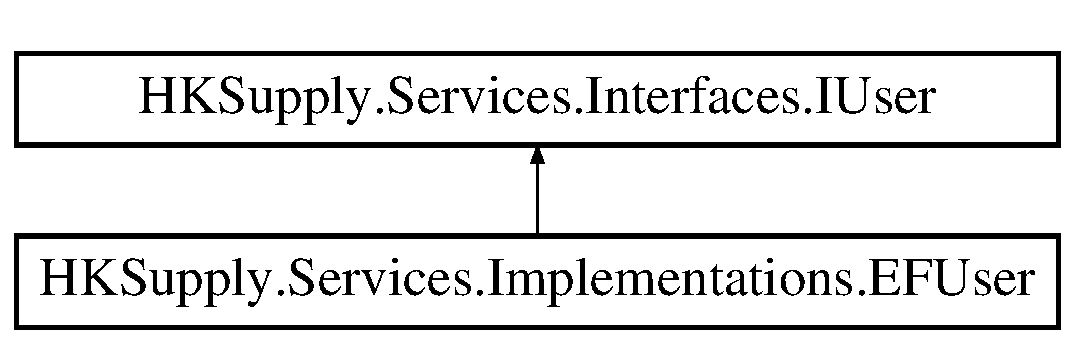
\includegraphics[height=2.000000cm]{class_h_k_supply_1_1_services_1_1_implementations_1_1_e_f_user}
\end{center}
\end{figure}
\subsection*{Public Member Functions}
\begin{DoxyCompactItemize}
\item 
I\+Enumerable$<$ \mbox{\hyperlink{class_h_k_supply_1_1_models_1_1_user}{User}} $>$ \mbox{\hyperlink{class_h_k_supply_1_1_services_1_1_implementations_1_1_e_f_user_a145638eeeb9e29780d17cbac23476a8d}{Get\+All\+Users}} ()
\begin{DoxyCompactList}\small\item\em Obtener la colección de usuarios del sistema \end{DoxyCompactList}\item 
\mbox{\hyperlink{class_h_k_supply_1_1_models_1_1_user}{User}} \mbox{\hyperlink{class_h_k_supply_1_1_services_1_1_implementations_1_1_e_f_user_a322969baaacbf15223b17f8117dd1545}{Get\+User\+By\+Id}} (int user\+Id)
\begin{DoxyCompactList}\small\item\em Obtener un usuario dado su id \end{DoxyCompactList}\item 
\mbox{\Hypertarget{class_h_k_supply_1_1_services_1_1_implementations_1_1_e_f_user_a330c2846df2d0fc7f7baa70889ebb3ed}\label{class_h_k_supply_1_1_services_1_1_implementations_1_1_e_f_user_a330c2846df2d0fc7f7baa70889ebb3ed}} 
\mbox{\hyperlink{class_h_k_supply_1_1_models_1_1_user}{User}} {\bfseries Get\+User\+By\+Login} (string user\+Login)
\item 
\mbox{\hyperlink{class_h_k_supply_1_1_models_1_1_user}{User}} \mbox{\hyperlink{class_h_k_supply_1_1_services_1_1_implementations_1_1_e_f_user_a69f04e0ab5ba947fc315c60abc7cdbf1}{Get\+User\+By\+Login\+Password}} (string User\+Login, string Password)
\begin{DoxyCompactList}\small\item\em Obtener un usuario dado un login y password \end{DoxyCompactList}\item 
\mbox{\hyperlink{class_h_k_supply_1_1_models_1_1_user}{User}} \mbox{\hyperlink{class_h_k_supply_1_1_services_1_1_implementations_1_1_e_f_user_a12abd287dc0491eed772d88b17fc9618}{New\+User}} (\mbox{\hyperlink{class_h_k_supply_1_1_models_1_1_user}{User}} new\+User)
\begin{DoxyCompactList}\small\item\em Dar de alta un usuario en el sistema \end{DoxyCompactList}\item 
bool \mbox{\hyperlink{class_h_k_supply_1_1_services_1_1_implementations_1_1_e_f_user_acb2996bf9f333684786d3e2d7b702ba4}{Disable\+User}} (string user\+Id, string remarks)
\begin{DoxyCompactList}\small\item\em Deshabilitar un usuario \end{DoxyCompactList}\item 
bool \mbox{\hyperlink{class_h_k_supply_1_1_services_1_1_implementations_1_1_e_f_user_ada8f9352d6fed7594d449aed92f452a0}{Change\+Password}} (int user\+Id, string password)
\begin{DoxyCompactList}\small\item\em Modidificar un password de un usuario \end{DoxyCompactList}\item 
bool \mbox{\hyperlink{class_h_k_supply_1_1_services_1_1_implementations_1_1_e_f_user_af7bbea584cce6ec7e2b8f4b4d46c01f6}{Update\+Users}} (I\+Enumerable$<$ \mbox{\hyperlink{class_h_k_supply_1_1_models_1_1_user}{User}} $>$ users\+To\+Update)
\begin{DoxyCompactList}\small\item\em Modificar una colección de usuarios. \end{DoxyCompactList}\end{DoxyCompactItemize}


\subsection{Detailed Description}
Controlador Entity Framework para user 



\subsection{Member Function Documentation}
\mbox{\Hypertarget{class_h_k_supply_1_1_services_1_1_implementations_1_1_e_f_user_ada8f9352d6fed7594d449aed92f452a0}\label{class_h_k_supply_1_1_services_1_1_implementations_1_1_e_f_user_ada8f9352d6fed7594d449aed92f452a0}} 
\index{H\+K\+Supply\+::\+Services\+::\+Implementations\+::\+E\+F\+User@{H\+K\+Supply\+::\+Services\+::\+Implementations\+::\+E\+F\+User}!Change\+Password@{Change\+Password}}
\index{Change\+Password@{Change\+Password}!H\+K\+Supply\+::\+Services\+::\+Implementations\+::\+E\+F\+User@{H\+K\+Supply\+::\+Services\+::\+Implementations\+::\+E\+F\+User}}
\subsubsection{\texorpdfstring{Change\+Password()}{ChangePassword()}}
{\footnotesize\ttfamily bool H\+K\+Supply.\+Services.\+Implementations.\+E\+F\+User.\+Change\+Password (\begin{DoxyParamCaption}\item[{int}]{user\+Id,  }\item[{string}]{password }\end{DoxyParamCaption})}



Modidificar un password de un usuario 


\begin{DoxyParams}{Parameters}
{\em user\+Id} & \\
\hline
{\em password} & \\
\hline
\end{DoxyParams}
\begin{DoxyReturn}{Returns}

\end{DoxyReturn}


Implements \mbox{\hyperlink{interface_h_k_supply_1_1_services_1_1_interfaces_1_1_i_user}{H\+K\+Supply.\+Services.\+Interfaces.\+I\+User}}.

\mbox{\Hypertarget{class_h_k_supply_1_1_services_1_1_implementations_1_1_e_f_user_acb2996bf9f333684786d3e2d7b702ba4}\label{class_h_k_supply_1_1_services_1_1_implementations_1_1_e_f_user_acb2996bf9f333684786d3e2d7b702ba4}} 
\index{H\+K\+Supply\+::\+Services\+::\+Implementations\+::\+E\+F\+User@{H\+K\+Supply\+::\+Services\+::\+Implementations\+::\+E\+F\+User}!Disable\+User@{Disable\+User}}
\index{Disable\+User@{Disable\+User}!H\+K\+Supply\+::\+Services\+::\+Implementations\+::\+E\+F\+User@{H\+K\+Supply\+::\+Services\+::\+Implementations\+::\+E\+F\+User}}
\subsubsection{\texorpdfstring{Disable\+User()}{DisableUser()}}
{\footnotesize\ttfamily bool H\+K\+Supply.\+Services.\+Implementations.\+E\+F\+User.\+Disable\+User (\begin{DoxyParamCaption}\item[{string}]{user\+Id,  }\item[{string}]{remarks }\end{DoxyParamCaption})}



Deshabilitar un usuario 


\begin{DoxyParams}{Parameters}
{\em user\+Id} & \\
\hline
{\em remarks} & \\
\hline
\end{DoxyParams}
\begin{DoxyReturn}{Returns}

\end{DoxyReturn}


Implements \mbox{\hyperlink{interface_h_k_supply_1_1_services_1_1_interfaces_1_1_i_user}{H\+K\+Supply.\+Services.\+Interfaces.\+I\+User}}.

\mbox{\Hypertarget{class_h_k_supply_1_1_services_1_1_implementations_1_1_e_f_user_a145638eeeb9e29780d17cbac23476a8d}\label{class_h_k_supply_1_1_services_1_1_implementations_1_1_e_f_user_a145638eeeb9e29780d17cbac23476a8d}} 
\index{H\+K\+Supply\+::\+Services\+::\+Implementations\+::\+E\+F\+User@{H\+K\+Supply\+::\+Services\+::\+Implementations\+::\+E\+F\+User}!Get\+All\+Users@{Get\+All\+Users}}
\index{Get\+All\+Users@{Get\+All\+Users}!H\+K\+Supply\+::\+Services\+::\+Implementations\+::\+E\+F\+User@{H\+K\+Supply\+::\+Services\+::\+Implementations\+::\+E\+F\+User}}
\subsubsection{\texorpdfstring{Get\+All\+Users()}{GetAllUsers()}}
{\footnotesize\ttfamily I\+Enumerable$<$\mbox{\hyperlink{class_h_k_supply_1_1_models_1_1_user}{User}}$>$ H\+K\+Supply.\+Services.\+Implementations.\+E\+F\+User.\+Get\+All\+Users (\begin{DoxyParamCaption}{ }\end{DoxyParamCaption})}



Obtener la colección de usuarios del sistema 

\begin{DoxyReturn}{Returns}

\end{DoxyReturn}


Implements \mbox{\hyperlink{interface_h_k_supply_1_1_services_1_1_interfaces_1_1_i_user}{H\+K\+Supply.\+Services.\+Interfaces.\+I\+User}}.

\mbox{\Hypertarget{class_h_k_supply_1_1_services_1_1_implementations_1_1_e_f_user_a322969baaacbf15223b17f8117dd1545}\label{class_h_k_supply_1_1_services_1_1_implementations_1_1_e_f_user_a322969baaacbf15223b17f8117dd1545}} 
\index{H\+K\+Supply\+::\+Services\+::\+Implementations\+::\+E\+F\+User@{H\+K\+Supply\+::\+Services\+::\+Implementations\+::\+E\+F\+User}!Get\+User\+By\+Id@{Get\+User\+By\+Id}}
\index{Get\+User\+By\+Id@{Get\+User\+By\+Id}!H\+K\+Supply\+::\+Services\+::\+Implementations\+::\+E\+F\+User@{H\+K\+Supply\+::\+Services\+::\+Implementations\+::\+E\+F\+User}}
\subsubsection{\texorpdfstring{Get\+User\+By\+Id()}{GetUserById()}}
{\footnotesize\ttfamily \mbox{\hyperlink{class_h_k_supply_1_1_models_1_1_user}{User}} H\+K\+Supply.\+Services.\+Implementations.\+E\+F\+User.\+Get\+User\+By\+Id (\begin{DoxyParamCaption}\item[{int}]{user\+Id }\end{DoxyParamCaption})}



Obtener un usuario dado su id 


\begin{DoxyParams}{Parameters}
{\em user\+Id} & \\
\hline
\end{DoxyParams}
\begin{DoxyReturn}{Returns}

\end{DoxyReturn}


Implements \mbox{\hyperlink{interface_h_k_supply_1_1_services_1_1_interfaces_1_1_i_user}{H\+K\+Supply.\+Services.\+Interfaces.\+I\+User}}.

\mbox{\Hypertarget{class_h_k_supply_1_1_services_1_1_implementations_1_1_e_f_user_a69f04e0ab5ba947fc315c60abc7cdbf1}\label{class_h_k_supply_1_1_services_1_1_implementations_1_1_e_f_user_a69f04e0ab5ba947fc315c60abc7cdbf1}} 
\index{H\+K\+Supply\+::\+Services\+::\+Implementations\+::\+E\+F\+User@{H\+K\+Supply\+::\+Services\+::\+Implementations\+::\+E\+F\+User}!Get\+User\+By\+Login\+Password@{Get\+User\+By\+Login\+Password}}
\index{Get\+User\+By\+Login\+Password@{Get\+User\+By\+Login\+Password}!H\+K\+Supply\+::\+Services\+::\+Implementations\+::\+E\+F\+User@{H\+K\+Supply\+::\+Services\+::\+Implementations\+::\+E\+F\+User}}
\subsubsection{\texorpdfstring{Get\+User\+By\+Login\+Password()}{GetUserByLoginPassword()}}
{\footnotesize\ttfamily \mbox{\hyperlink{class_h_k_supply_1_1_models_1_1_user}{User}} H\+K\+Supply.\+Services.\+Implementations.\+E\+F\+User.\+Get\+User\+By\+Login\+Password (\begin{DoxyParamCaption}\item[{string}]{User\+Login,  }\item[{string}]{Password }\end{DoxyParamCaption})}



Obtener un usuario dado un login y password 


\begin{DoxyParams}{Parameters}
{\em User\+Login} & \\
\hline
{\em Password} & \\
\hline
\end{DoxyParams}
\begin{DoxyReturn}{Returns}

\end{DoxyReturn}


Implements \mbox{\hyperlink{interface_h_k_supply_1_1_services_1_1_interfaces_1_1_i_user}{H\+K\+Supply.\+Services.\+Interfaces.\+I\+User}}.

\mbox{\Hypertarget{class_h_k_supply_1_1_services_1_1_implementations_1_1_e_f_user_a12abd287dc0491eed772d88b17fc9618}\label{class_h_k_supply_1_1_services_1_1_implementations_1_1_e_f_user_a12abd287dc0491eed772d88b17fc9618}} 
\index{H\+K\+Supply\+::\+Services\+::\+Implementations\+::\+E\+F\+User@{H\+K\+Supply\+::\+Services\+::\+Implementations\+::\+E\+F\+User}!New\+User@{New\+User}}
\index{New\+User@{New\+User}!H\+K\+Supply\+::\+Services\+::\+Implementations\+::\+E\+F\+User@{H\+K\+Supply\+::\+Services\+::\+Implementations\+::\+E\+F\+User}}
\subsubsection{\texorpdfstring{New\+User()}{NewUser()}}
{\footnotesize\ttfamily \mbox{\hyperlink{class_h_k_supply_1_1_models_1_1_user}{User}} H\+K\+Supply.\+Services.\+Implementations.\+E\+F\+User.\+New\+User (\begin{DoxyParamCaption}\item[{\mbox{\hyperlink{class_h_k_supply_1_1_models_1_1_user}{User}}}]{new\+User }\end{DoxyParamCaption})}



Dar de alta un usuario en el sistema 


\begin{DoxyParams}{Parameters}
{\em new\+User} & \\
\hline
\end{DoxyParams}
\begin{DoxyReturn}{Returns}

\end{DoxyReturn}


Implements \mbox{\hyperlink{interface_h_k_supply_1_1_services_1_1_interfaces_1_1_i_user}{H\+K\+Supply.\+Services.\+Interfaces.\+I\+User}}.

\mbox{\Hypertarget{class_h_k_supply_1_1_services_1_1_implementations_1_1_e_f_user_af7bbea584cce6ec7e2b8f4b4d46c01f6}\label{class_h_k_supply_1_1_services_1_1_implementations_1_1_e_f_user_af7bbea584cce6ec7e2b8f4b4d46c01f6}} 
\index{H\+K\+Supply\+::\+Services\+::\+Implementations\+::\+E\+F\+User@{H\+K\+Supply\+::\+Services\+::\+Implementations\+::\+E\+F\+User}!Update\+Users@{Update\+Users}}
\index{Update\+Users@{Update\+Users}!H\+K\+Supply\+::\+Services\+::\+Implementations\+::\+E\+F\+User@{H\+K\+Supply\+::\+Services\+::\+Implementations\+::\+E\+F\+User}}
\subsubsection{\texorpdfstring{Update\+Users()}{UpdateUsers()}}
{\footnotesize\ttfamily bool H\+K\+Supply.\+Services.\+Implementations.\+E\+F\+User.\+Update\+Users (\begin{DoxyParamCaption}\item[{I\+Enumerable$<$ \mbox{\hyperlink{class_h_k_supply_1_1_models_1_1_user}{User}} $>$}]{users\+To\+Update }\end{DoxyParamCaption})}



Modificar una colección de usuarios. 


\begin{DoxyParams}{Parameters}
{\em users\+To\+Update} & \\
\hline
\end{DoxyParams}
\begin{DoxyReturn}{Returns}

\end{DoxyReturn}


Los campos que se modifican son los siguientes\+:
\begin{DoxyItemize}
\item Name
\item Role\+Id
\item Enabled
\item Remarks 
\end{DoxyItemize}

Implements \mbox{\hyperlink{interface_h_k_supply_1_1_services_1_1_interfaces_1_1_i_user}{H\+K\+Supply.\+Services.\+Interfaces.\+I\+User}}.



The documentation for this class was generated from the following file\+:\begin{DoxyCompactItemize}
\item 
H\+K\+Supply/\+Services/\+Implementations/E\+F\+User.\+cs\end{DoxyCompactItemize}

\hypertarget{class_h_k_supply_1_1_form1}{}\section{H\+K\+Supply.\+Form1 Class Reference}
\label{class_h_k_supply_1_1_form1}\index{H\+K\+Supply.\+Form1@{H\+K\+Supply.\+Form1}}
Inheritance diagram for H\+K\+Supply.\+Form1\+:\begin{figure}[H]
\begin{center}
\leavevmode
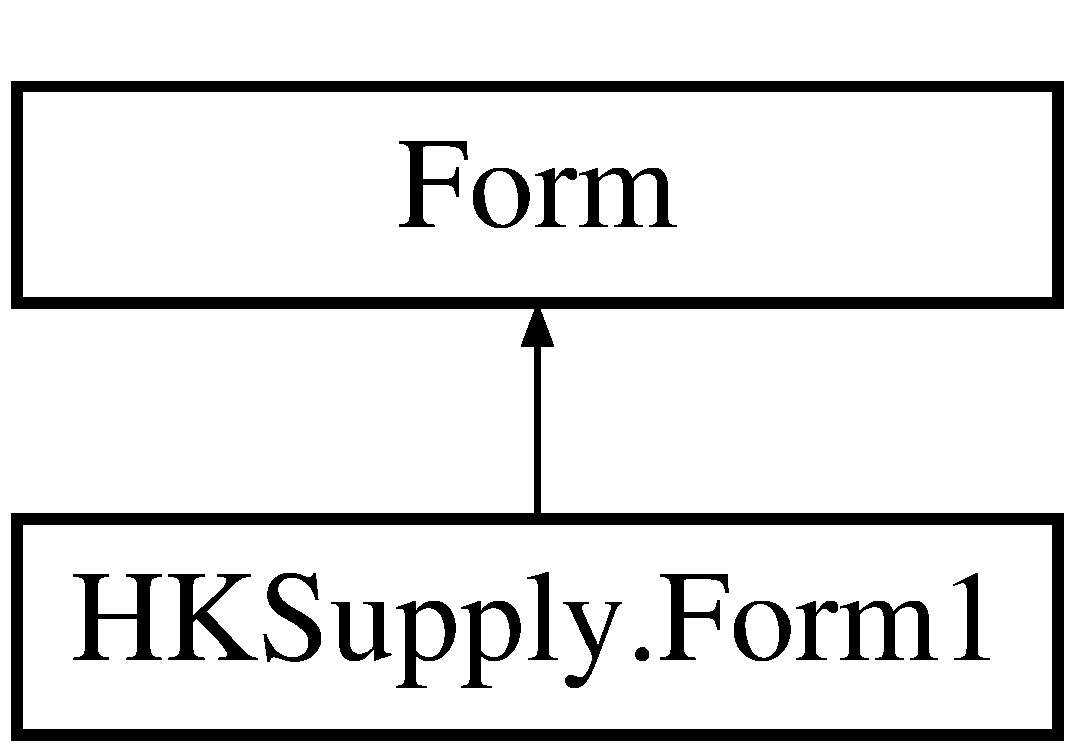
\includegraphics[height=2.000000cm]{class_h_k_supply_1_1_form1}
\end{center}
\end{figure}
\subsection*{Protected Member Functions}
\begin{DoxyCompactItemize}
\item 
override void \mbox{\hyperlink{class_h_k_supply_1_1_form1_a406b8a9257d093c285ba546b75e81757}{Dispose}} (bool disposing)
\begin{DoxyCompactList}\small\item\em Limpiar los recursos que se estén utilizando. \end{DoxyCompactList}\end{DoxyCompactItemize}


\subsection{Member Function Documentation}
\mbox{\Hypertarget{class_h_k_supply_1_1_form1_a406b8a9257d093c285ba546b75e81757}\label{class_h_k_supply_1_1_form1_a406b8a9257d093c285ba546b75e81757}} 
\index{H\+K\+Supply\+::\+Form1@{H\+K\+Supply\+::\+Form1}!Dispose@{Dispose}}
\index{Dispose@{Dispose}!H\+K\+Supply\+::\+Form1@{H\+K\+Supply\+::\+Form1}}
\subsubsection{\texorpdfstring{Dispose()}{Dispose()}}
{\footnotesize\ttfamily override void H\+K\+Supply.\+Form1.\+Dispose (\begin{DoxyParamCaption}\item[{bool}]{disposing }\end{DoxyParamCaption})\hspace{0.3cm}{\ttfamily [protected]}}



Limpiar los recursos que se estén utilizando. 


\begin{DoxyParams}{Parameters}
{\em disposing} & true si los recursos administrados se deben eliminar; false en caso contrario.\\
\hline
\end{DoxyParams}


The documentation for this class was generated from the following files\+:\begin{DoxyCompactItemize}
\item 
H\+K\+Supply/Form1.\+cs\item 
H\+K\+Supply/Form1.\+Designer.\+cs\end{DoxyCompactItemize}

\hypertarget{class_h_k_supply_1_1_models_1_1_functionality}{}\section{H\+K\+Supply.\+Models.\+Functionality Class Reference}
\label{class_h_k_supply_1_1_models_1_1_functionality}\index{H\+K\+Supply.\+Models.\+Functionality@{H\+K\+Supply.\+Models.\+Functionality}}
\subsection*{Public Member Functions}
\begin{DoxyCompactItemize}
\item 
\mbox{\Hypertarget{class_h_k_supply_1_1_models_1_1_functionality_a335165c2bd6cbc5ff6d314cb03d70246}\label{class_h_k_supply_1_1_models_1_1_functionality_a335165c2bd6cbc5ff6d314cb03d70246}} 
override bool {\bfseries Equals} (object obj)
\item 
\mbox{\Hypertarget{class_h_k_supply_1_1_models_1_1_functionality_ad460dce69ed01477901c5ac1e2abcd89}\label{class_h_k_supply_1_1_models_1_1_functionality_ad460dce69ed01477901c5ac1e2abcd89}} 
override int {\bfseries Get\+Hash\+Code} ()
\end{DoxyCompactItemize}
\subsection*{Properties}
\begin{DoxyCompactItemize}
\item 
\mbox{\Hypertarget{class_h_k_supply_1_1_models_1_1_functionality_a1d4863a80797dc71a680cdfb1981622f}\label{class_h_k_supply_1_1_models_1_1_functionality_a1d4863a80797dc71a680cdfb1981622f}} 
int {\bfseries Functionality\+Id}\hspace{0.3cm}{\ttfamily  \mbox{[}get, set\mbox{]}}
\item 
\mbox{\Hypertarget{class_h_k_supply_1_1_models_1_1_functionality_ab33c1a395b442de1c096c8beb00ab968}\label{class_h_k_supply_1_1_models_1_1_functionality_ab33c1a395b442de1c096c8beb00ab968}} 
string {\bfseries Functionality\+Name}\hspace{0.3cm}{\ttfamily  \mbox{[}get, set\mbox{]}}
\item 
\mbox{\Hypertarget{class_h_k_supply_1_1_models_1_1_functionality_a435984473f4cb370eab0a72efa561c1a}\label{class_h_k_supply_1_1_models_1_1_functionality_a435984473f4cb370eab0a72efa561c1a}} 
string {\bfseries Category}\hspace{0.3cm}{\ttfamily  \mbox{[}get, set\mbox{]}}
\item 
\mbox{\Hypertarget{class_h_k_supply_1_1_models_1_1_functionality_a23ca4563c106add51c24a2741bf946a1}\label{class_h_k_supply_1_1_models_1_1_functionality_a23ca4563c106add51c24a2741bf946a1}} 
string {\bfseries Form\+Name}\hspace{0.3cm}{\ttfamily  \mbox{[}get, set\mbox{]}}
\end{DoxyCompactItemize}


The documentation for this class was generated from the following file\+:\begin{DoxyCompactItemize}
\item 
H\+K\+Supply/\+Models/Functionality.\+cs\end{DoxyCompactItemize}

\hypertarget{class_h_k_supply_1_1_forms_1_1_master_1_1_functionality_management}{}\section{H\+K\+Supply.\+Forms.\+Master.\+Functionality\+Management Class Reference}
\label{class_h_k_supply_1_1_forms_1_1_master_1_1_functionality_management}\index{H\+K\+Supply.\+Forms.\+Master.\+Functionality\+Management@{H\+K\+Supply.\+Forms.\+Master.\+Functionality\+Management}}
Inheritance diagram for H\+K\+Supply.\+Forms.\+Master.\+Functionality\+Management\+:\begin{figure}[H]
\begin{center}
\leavevmode
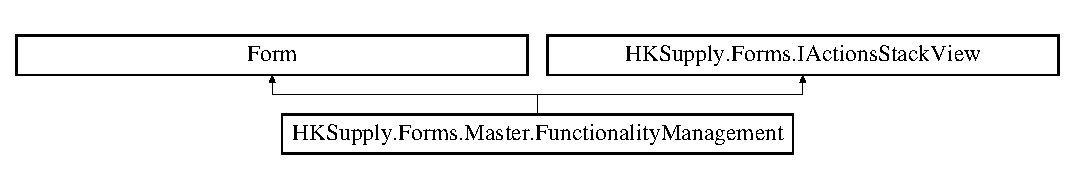
\includegraphics[height=1.830065cm]{class_h_k_supply_1_1_forms_1_1_master_1_1_functionality_management}
\end{center}
\end{figure}
\subsection*{Public Member Functions}
\begin{DoxyCompactItemize}
\item 
\mbox{\Hypertarget{class_h_k_supply_1_1_forms_1_1_master_1_1_functionality_management_a3d72cc9c48dd79d936535dbb386ca304}\label{class_h_k_supply_1_1_forms_1_1_master_1_1_functionality_management_a3d72cc9c48dd79d936535dbb386ca304}} 
void {\bfseries actions\+Stack\+View\+\_\+\+Edit\+Button\+Click} (object sender, Event\+Args e)
\item 
\mbox{\Hypertarget{class_h_k_supply_1_1_forms_1_1_master_1_1_functionality_management_a124bbeebef7a1f06573a032342571c8f}\label{class_h_k_supply_1_1_forms_1_1_master_1_1_functionality_management_a124bbeebef7a1f06573a032342571c8f}} 
void {\bfseries actions\+Stack\+View\+\_\+\+New\+Button\+Click} (object sender, Event\+Args e)
\item 
\mbox{\Hypertarget{class_h_k_supply_1_1_forms_1_1_master_1_1_functionality_management_a775ec1a63caa9faf229f704d14bd11a5}\label{class_h_k_supply_1_1_forms_1_1_master_1_1_functionality_management_a775ec1a63caa9faf229f704d14bd11a5}} 
void {\bfseries actions\+Stack\+View\+\_\+\+Save\+Button\+Click} (object sender, Event\+Args e)
\item 
\mbox{\Hypertarget{class_h_k_supply_1_1_forms_1_1_master_1_1_functionality_management_a7bcf668b3f862d8ee0c60ef08e2075ff}\label{class_h_k_supply_1_1_forms_1_1_master_1_1_functionality_management_a7bcf668b3f862d8ee0c60ef08e2075ff}} 
void {\bfseries actions\+Stack\+View\+\_\+\+Cancel\+Button\+Click} (object sender, Event\+Args e)
\item 
\mbox{\Hypertarget{class_h_k_supply_1_1_forms_1_1_master_1_1_functionality_management_a5c2909260f97b980620f3a81bf9aaa5a}\label{class_h_k_supply_1_1_forms_1_1_master_1_1_functionality_management_a5c2909260f97b980620f3a81bf9aaa5a}} 
void {\bfseries Configure\+Actions\+Stack\+View} ()
\end{DoxyCompactItemize}
\subsection*{Protected Member Functions}
\begin{DoxyCompactItemize}
\item 
override void \hyperlink{class_h_k_supply_1_1_forms_1_1_master_1_1_functionality_management_a36e30f6560cd85f1d5369dadd79487d4}{Dispose} (bool disposing)
\begin{DoxyCompactList}\small\item\em Clean up any resources being used. \end{DoxyCompactList}\end{DoxyCompactItemize}


\subsection{Member Function Documentation}
\mbox{\Hypertarget{class_h_k_supply_1_1_forms_1_1_master_1_1_functionality_management_a36e30f6560cd85f1d5369dadd79487d4}\label{class_h_k_supply_1_1_forms_1_1_master_1_1_functionality_management_a36e30f6560cd85f1d5369dadd79487d4}} 
\index{H\+K\+Supply\+::\+Forms\+::\+Master\+::\+Functionality\+Management@{H\+K\+Supply\+::\+Forms\+::\+Master\+::\+Functionality\+Management}!Dispose@{Dispose}}
\index{Dispose@{Dispose}!H\+K\+Supply\+::\+Forms\+::\+Master\+::\+Functionality\+Management@{H\+K\+Supply\+::\+Forms\+::\+Master\+::\+Functionality\+Management}}
\subsubsection{\texorpdfstring{Dispose()}{Dispose()}}
{\footnotesize\ttfamily override void H\+K\+Supply.\+Forms.\+Master.\+Functionality\+Management.\+Dispose (\begin{DoxyParamCaption}\item[{bool}]{disposing }\end{DoxyParamCaption})\hspace{0.3cm}{\ttfamily [protected]}}



Clean up any resources being used. 


\begin{DoxyParams}{Parameters}
{\em disposing} & true if managed resources should be disposed; otherwise, false.\\
\hline
\end{DoxyParams}


The documentation for this class was generated from the following files\+:\begin{DoxyCompactItemize}
\item 
H\+K\+Supply/\+Forms/\+Master/Functionality\+Management.\+cs\item 
H\+K\+Supply/\+Forms/\+Master/Functionality\+Management.\+Designer.\+cs\end{DoxyCompactItemize}

\hypertarget{class_h_k_supply_1_1_models_1_1_functionality_role}{}\section{H\+K\+Supply.\+Models.\+Functionality\+Role Class Reference}
\label{class_h_k_supply_1_1_models_1_1_functionality_role}\index{H\+K\+Supply.\+Models.\+Functionality\+Role@{H\+K\+Supply.\+Models.\+Functionality\+Role}}
\subsection*{Public Member Functions}
\begin{DoxyCompactItemize}
\item 
\mbox{\Hypertarget{class_h_k_supply_1_1_models_1_1_functionality_role_a7d1146c2bece3c191ab8a8cbb8bd48b6}\label{class_h_k_supply_1_1_models_1_1_functionality_role_a7d1146c2bece3c191ab8a8cbb8bd48b6}} 
override bool {\bfseries Equals} (object obj)
\item 
\mbox{\Hypertarget{class_h_k_supply_1_1_models_1_1_functionality_role_aeab06b31e0fadbbb24099c8b0cad850c}\label{class_h_k_supply_1_1_models_1_1_functionality_role_aeab06b31e0fadbbb24099c8b0cad850c}} 
override int {\bfseries Get\+Hash\+Code} ()
\end{DoxyCompactItemize}
\subsection*{Properties}
\begin{DoxyCompactItemize}
\item 
\mbox{\Hypertarget{class_h_k_supply_1_1_models_1_1_functionality_role_a0ded12aa8bec42c6b7bb6097c74c35e7}\label{class_h_k_supply_1_1_models_1_1_functionality_role_a0ded12aa8bec42c6b7bb6097c74c35e7}} 
int {\bfseries Functionality\+Id}\hspace{0.3cm}{\ttfamily  \mbox{[}get, set\mbox{]}}
\item 
\mbox{\Hypertarget{class_h_k_supply_1_1_models_1_1_functionality_role_a765b8678a9661752e6f2899d98e661d4}\label{class_h_k_supply_1_1_models_1_1_functionality_role_a765b8678a9661752e6f2899d98e661d4}} 
string {\bfseries Role\+Id}\hspace{0.3cm}{\ttfamily  \mbox{[}get, set\mbox{]}}
\item 
\mbox{\Hypertarget{class_h_k_supply_1_1_models_1_1_functionality_role_aed71c97ac0caf396dc15a24c45d56fab}\label{class_h_k_supply_1_1_models_1_1_functionality_role_aed71c97ac0caf396dc15a24c45d56fab}} 
bool {\bfseries Read}\hspace{0.3cm}{\ttfamily  \mbox{[}get, set\mbox{]}}
\item 
\mbox{\Hypertarget{class_h_k_supply_1_1_models_1_1_functionality_role_a6faad04d06f87ef7121acb504c3c6759}\label{class_h_k_supply_1_1_models_1_1_functionality_role_a6faad04d06f87ef7121acb504c3c6759}} 
bool {\bfseries New}\hspace{0.3cm}{\ttfamily  \mbox{[}get, set\mbox{]}}
\item 
\mbox{\Hypertarget{class_h_k_supply_1_1_models_1_1_functionality_role_a26b7d361ba1ab93b2f393b1b99e5fc39}\label{class_h_k_supply_1_1_models_1_1_functionality_role_a26b7d361ba1ab93b2f393b1b99e5fc39}} 
bool {\bfseries Modify}\hspace{0.3cm}{\ttfamily  \mbox{[}get, set\mbox{]}}
\item 
\mbox{\Hypertarget{class_h_k_supply_1_1_models_1_1_functionality_role_ae6697fdcf6d2cdcbcf86736b5abbc3ae}\label{class_h_k_supply_1_1_models_1_1_functionality_role_ae6697fdcf6d2cdcbcf86736b5abbc3ae}} 
\mbox{\hyperlink{class_h_k_supply_1_1_models_1_1_functionality}{Functionality}} {\bfseries Functionality}\hspace{0.3cm}{\ttfamily  \mbox{[}get, set\mbox{]}}
\item 
\mbox{\Hypertarget{class_h_k_supply_1_1_models_1_1_functionality_role_a94917c7d388484877ef08df62449f747}\label{class_h_k_supply_1_1_models_1_1_functionality_role_a94917c7d388484877ef08df62449f747}} 
\mbox{\hyperlink{class_h_k_supply_1_1_models_1_1_role}{Role}} {\bfseries Role}\hspace{0.3cm}{\ttfamily  \mbox{[}get, set\mbox{]}}
\end{DoxyCompactItemize}


The documentation for this class was generated from the following file\+:\begin{DoxyCompactItemize}
\item 
H\+K\+Supply/\+Models/Functionality\+Role.\+cs\end{DoxyCompactItemize}

\hypertarget{class_h_k_supply_1_1_forms_1_1_master_1_1_functionality_role_management}{}\section{H\+K\+Supply.\+Forms.\+Master.\+Functionality\+Role\+Management Class Reference}
\label{class_h_k_supply_1_1_forms_1_1_master_1_1_functionality_role_management}\index{H\+K\+Supply.\+Forms.\+Master.\+Functionality\+Role\+Management@{H\+K\+Supply.\+Forms.\+Master.\+Functionality\+Role\+Management}}
Inheritance diagram for H\+K\+Supply.\+Forms.\+Master.\+Functionality\+Role\+Management\+:\begin{figure}[H]
\begin{center}
\leavevmode
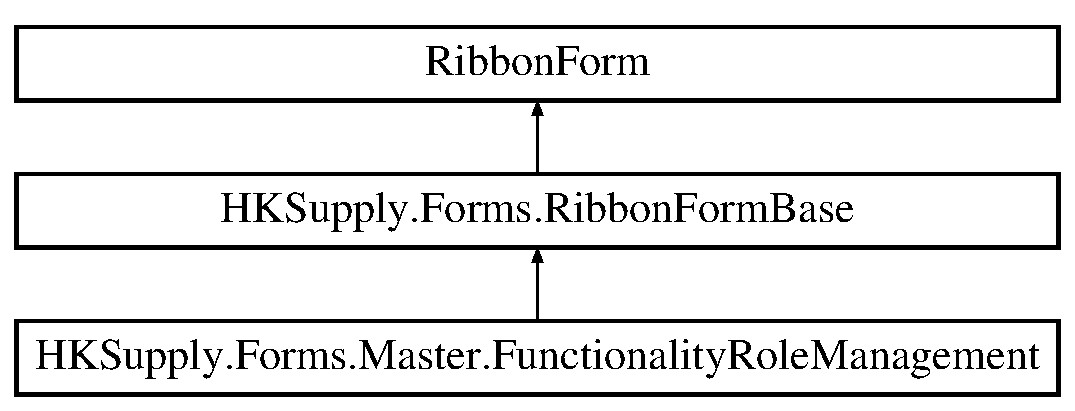
\includegraphics[height=1.691843cm]{class_h_k_supply_1_1_forms_1_1_master_1_1_functionality_role_management}
\end{center}
\end{figure}
\subsection*{Public Member Functions}
\begin{DoxyCompactItemize}
\item 
\mbox{\Hypertarget{class_h_k_supply_1_1_forms_1_1_master_1_1_functionality_role_management_ad8f36ecae11021e4d8d2f5b06de7b881}\label{class_h_k_supply_1_1_forms_1_1_master_1_1_functionality_role_management_ad8f36ecae11021e4d8d2f5b06de7b881}} 
void {\bfseries actions\+Stack\+View\+\_\+\+Edit\+Button\+Click} (object sender, Event\+Args e)
\item 
\mbox{\Hypertarget{class_h_k_supply_1_1_forms_1_1_master_1_1_functionality_role_management_a3bed94c9724e4256dd85fcc8d4c2f276}\label{class_h_k_supply_1_1_forms_1_1_master_1_1_functionality_role_management_a3bed94c9724e4256dd85fcc8d4c2f276}} 
void {\bfseries actions\+Stack\+View\+\_\+\+New\+Button\+Click} (object sender, Event\+Args e)
\item 
\mbox{\Hypertarget{class_h_k_supply_1_1_forms_1_1_master_1_1_functionality_role_management_a8aed80ca8eb88d632fa3501141f4399d}\label{class_h_k_supply_1_1_forms_1_1_master_1_1_functionality_role_management_a8aed80ca8eb88d632fa3501141f4399d}} 
void {\bfseries actions\+Stack\+View\+\_\+\+Save\+Button\+Click} (object sender, Event\+Args e)
\item 
\mbox{\Hypertarget{class_h_k_supply_1_1_forms_1_1_master_1_1_functionality_role_management_a00fc25391f0a3d782823871e2d897b4b}\label{class_h_k_supply_1_1_forms_1_1_master_1_1_functionality_role_management_a00fc25391f0a3d782823871e2d897b4b}} 
void {\bfseries actions\+Stack\+View\+\_\+\+Cancel\+Button\+Click} (object sender, Event\+Args e)
\item 
\mbox{\Hypertarget{class_h_k_supply_1_1_forms_1_1_master_1_1_functionality_role_management_adcf6dece3abda929fb54cec2bec5a708}\label{class_h_k_supply_1_1_forms_1_1_master_1_1_functionality_role_management_adcf6dece3abda929fb54cec2bec5a708}} 
void {\bfseries Configure\+Actions\+Stack\+View} ()
\end{DoxyCompactItemize}
\subsection*{Protected Member Functions}
\begin{DoxyCompactItemize}
\item 
override void \hyperlink{class_h_k_supply_1_1_forms_1_1_master_1_1_functionality_role_management_a9a7c00e015e462fba8baf1e25be79413}{Dispose} (bool disposing)
\begin{DoxyCompactList}\small\item\em Clean up any resources being used. \end{DoxyCompactList}\end{DoxyCompactItemize}


\subsection{Member Function Documentation}
\mbox{\Hypertarget{class_h_k_supply_1_1_forms_1_1_master_1_1_functionality_role_management_a9a7c00e015e462fba8baf1e25be79413}\label{class_h_k_supply_1_1_forms_1_1_master_1_1_functionality_role_management_a9a7c00e015e462fba8baf1e25be79413}} 
\index{H\+K\+Supply\+::\+Forms\+::\+Master\+::\+Functionality\+Role\+Management@{H\+K\+Supply\+::\+Forms\+::\+Master\+::\+Functionality\+Role\+Management}!Dispose@{Dispose}}
\index{Dispose@{Dispose}!H\+K\+Supply\+::\+Forms\+::\+Master\+::\+Functionality\+Role\+Management@{H\+K\+Supply\+::\+Forms\+::\+Master\+::\+Functionality\+Role\+Management}}
\subsubsection{\texorpdfstring{Dispose()}{Dispose()}}
{\footnotesize\ttfamily override void H\+K\+Supply.\+Forms.\+Master.\+Functionality\+Role\+Management.\+Dispose (\begin{DoxyParamCaption}\item[{bool}]{disposing }\end{DoxyParamCaption})\hspace{0.3cm}{\ttfamily [protected]}}



Clean up any resources being used. 


\begin{DoxyParams}{Parameters}
{\em disposing} & true if managed resources should be disposed; otherwise, false.\\
\hline
\end{DoxyParams}


The documentation for this class was generated from the following files\+:\begin{DoxyCompactItemize}
\item 
H\+K\+Supply/\+Forms/\+Master/Functionality\+Role\+Management.\+cs\item 
H\+K\+Supply/\+Forms/\+Master/Functionality\+Role\+Management.\+Designer.\+cs\end{DoxyCompactItemize}

\hypertarget{class_h_k_suply_1_1_unit_test_1_1_functionality_role_test}{}\section{H\+K\+Suply.\+Unit\+Test.\+Functionality\+Role\+Test Class Reference}
\label{class_h_k_suply_1_1_unit_test_1_1_functionality_role_test}\index{H\+K\+Suply.\+Unit\+Test.\+Functionality\+Role\+Test@{H\+K\+Suply.\+Unit\+Test.\+Functionality\+Role\+Test}}
\subsection*{Public Member Functions}
\begin{DoxyCompactItemize}
\item 
\mbox{\Hypertarget{class_h_k_suply_1_1_unit_test_1_1_functionality_role_test_ac133f39d498aea4477fca5c33a68fdcc}\label{class_h_k_suply_1_1_unit_test_1_1_functionality_role_test_ac133f39d498aea4477fca5c33a68fdcc}} 
void {\bfseries Get\+All\+Functionalities\+Role} ()
\item 
\mbox{\Hypertarget{class_h_k_suply_1_1_unit_test_1_1_functionality_role_test_a6be3df22cff2086d466362562a424849}\label{class_h_k_suply_1_1_unit_test_1_1_functionality_role_test_a6be3df22cff2086d466362562a424849}} 
void {\bfseries Get\+Functionality\+Role} ()
\item 
\mbox{\Hypertarget{class_h_k_suply_1_1_unit_test_1_1_functionality_role_test_a2939d4000f716e0577656a9526322edb}\label{class_h_k_suply_1_1_unit_test_1_1_functionality_role_test_a2939d4000f716e0577656a9526322edb}} 
void {\bfseries Get\+Functionalities\+Role} ()
\item 
\mbox{\Hypertarget{class_h_k_suply_1_1_unit_test_1_1_functionality_role_test_aa181b9200ffbd3b2a39d7c4eea17d546}\label{class_h_k_suply_1_1_unit_test_1_1_functionality_role_test_aa181b9200ffbd3b2a39d7c4eea17d546}} 
void {\bfseries Get\+Functionalities\+Categories\+Role} ()
\item 
\mbox{\Hypertarget{class_h_k_suply_1_1_unit_test_1_1_functionality_role_test_a044c261bef5cd0575d11799bd86961af}\label{class_h_k_suply_1_1_unit_test_1_1_functionality_role_test_a044c261bef5cd0575d11799bd86961af}} 
void {\bfseries New\+Functionality\+Role} ()
\item 
\mbox{\Hypertarget{class_h_k_suply_1_1_unit_test_1_1_functionality_role_test_a7fd10863dba59d604f1bf79382901267}\label{class_h_k_suply_1_1_unit_test_1_1_functionality_role_test_a7fd10863dba59d604f1bf79382901267}} 
void {\bfseries Modify\+Functionality\+Role} ()
\item 
\mbox{\Hypertarget{class_h_k_suply_1_1_unit_test_1_1_functionality_role_test_a162e2ece0babea12354c0930f4c77079}\label{class_h_k_suply_1_1_unit_test_1_1_functionality_role_test_a162e2ece0babea12354c0930f4c77079}} 
void {\bfseries Update\+Functionalities\+Roles} ()
\end{DoxyCompactItemize}


The documentation for this class was generated from the following file\+:\begin{DoxyCompactItemize}
\item 
H\+K\+Suply.\+Unit\+Test/Functionality\+Role\+Test.\+cs\end{DoxyCompactItemize}

\hypertarget{class_h_k_suply_1_1_unit_test_1_1_functionality_test}{}\section{H\+K\+Suply.\+Unit\+Test.\+Functionality\+Test Class Reference}
\label{class_h_k_suply_1_1_unit_test_1_1_functionality_test}\index{H\+K\+Suply.\+Unit\+Test.\+Functionality\+Test@{H\+K\+Suply.\+Unit\+Test.\+Functionality\+Test}}
\subsection*{Public Member Functions}
\begin{DoxyCompactItemize}
\item 
\mbox{\Hypertarget{class_h_k_suply_1_1_unit_test_1_1_functionality_test_a7c1c4dbb73d76537cee7110a85011bdb}\label{class_h_k_suply_1_1_unit_test_1_1_functionality_test_a7c1c4dbb73d76537cee7110a85011bdb}} 
void {\bfseries Get\+Functionality} ()
\item 
\mbox{\Hypertarget{class_h_k_suply_1_1_unit_test_1_1_functionality_test_ac8505a9a8bb7353e45e84ab7ee68c8fb}\label{class_h_k_suply_1_1_unit_test_1_1_functionality_test_ac8505a9a8bb7353e45e84ab7ee68c8fb}} 
void {\bfseries New\+Functionality} ()
\item 
\mbox{\Hypertarget{class_h_k_suply_1_1_unit_test_1_1_functionality_test_a7c1c86aff37c2c7d23c8c48e10df6425}\label{class_h_k_suply_1_1_unit_test_1_1_functionality_test_a7c1c86aff37c2c7d23c8c48e10df6425}} 
void {\bfseries Update\+Functionality} ()
\end{DoxyCompactItemize}


The documentation for this class was generated from the following file\+:\begin{DoxyCompactItemize}
\item 
H\+K\+Suply.\+Unit\+Test/Functionality\+Test.\+cs\end{DoxyCompactItemize}

\hypertarget{class_h_k_supply_1_1_general_1_1_global_setting}{}\section{H\+K\+Supply.\+General.\+Global\+Setting Class Reference}
\label{class_h_k_supply_1_1_general_1_1_global_setting}\index{H\+K\+Supply.\+General.\+Global\+Setting@{H\+K\+Supply.\+General.\+Global\+Setting}}


Objeto para guardar valores globales accesibles desde toda la aplicación.  


\subsection*{Properties}
\begin{DoxyCompactItemize}
\item 
\mbox{\Hypertarget{class_h_k_supply_1_1_general_1_1_global_setting_a6bfb54fe6ce82b0427c93287f3174fcc}\label{class_h_k_supply_1_1_general_1_1_global_setting_a6bfb54fe6ce82b0427c93287f3174fcc}} 
static \hyperlink{interface_h_k_supply_1_1_services_1_1_interfaces_1_1_i_role}{I\+Role} {\bfseries Role\+Service}\hspace{0.3cm}{\ttfamily  \mbox{[}get\mbox{]}}
\item 
\mbox{\Hypertarget{class_h_k_supply_1_1_general_1_1_global_setting_afcf3f82e4605ee135bef3b76601faef8}\label{class_h_k_supply_1_1_general_1_1_global_setting_afcf3f82e4605ee135bef3b76601faef8}} 
static \hyperlink{interface_h_k_supply_1_1_services_1_1_interfaces_1_1_i_user}{I\+User} {\bfseries User\+Service}\hspace{0.3cm}{\ttfamily  \mbox{[}get\mbox{]}}
\item 
\mbox{\Hypertarget{class_h_k_supply_1_1_general_1_1_global_setting_aa4423c9bf929f499c03e32ebee39d7bc}\label{class_h_k_supply_1_1_general_1_1_global_setting_aa4423c9bf929f499c03e32ebee39d7bc}} 
static \hyperlink{interface_h_k_supply_1_1_services_1_1_interfaces_1_1_i_functionality}{I\+Functionality} {\bfseries Functionality\+Service}\hspace{0.3cm}{\ttfamily  \mbox{[}get\mbox{]}}
\item 
\mbox{\Hypertarget{class_h_k_supply_1_1_general_1_1_global_setting_a6e0c94569c8e737d382725931c272390}\label{class_h_k_supply_1_1_general_1_1_global_setting_a6e0c94569c8e737d382725931c272390}} 
static \hyperlink{interface_h_k_supply_1_1_services_1_1_interfaces_1_1_i_functionality_role}{I\+Functionality\+Role} {\bfseries Functionality\+Role\+Service}\hspace{0.3cm}{\ttfamily  \mbox{[}get\mbox{]}}
\item 
\mbox{\Hypertarget{class_h_k_supply_1_1_general_1_1_global_setting_adeb470418d2461437e6dc55fd41f78f5}\label{class_h_k_supply_1_1_general_1_1_global_setting_adeb470418d2461437e6dc55fd41f78f5}} 
static \hyperlink{class_h_k_supply_1_1_models_1_1_user}{User} {\bfseries Logged\+User}\hspace{0.3cm}{\ttfamily  \mbox{[}get, set\mbox{]}}
\item 
\mbox{\Hypertarget{class_h_k_supply_1_1_general_1_1_global_setting_adf54b9c3d32b3dac949776dee6f17eb2}\label{class_h_k_supply_1_1_general_1_1_global_setting_adf54b9c3d32b3dac949776dee6f17eb2}} 
static I\+Enumerable$<$ \hyperlink{class_h_k_supply_1_1_models_1_1_functionality_role}{Functionality\+Role} $>$ {\bfseries Functionalities\+Roles}\hspace{0.3cm}{\ttfamily  \mbox{[}get, set\mbox{]}}
\item 
\mbox{\Hypertarget{class_h_k_supply_1_1_general_1_1_global_setting_ad2628f5f55a5a8f640cd28aa425f968f}\label{class_h_k_supply_1_1_general_1_1_global_setting_ad2628f5f55a5a8f640cd28aa425f968f}} 
static Resource\+Manager {\bfseries Res\+Manager}\hspace{0.3cm}{\ttfamily  \mbox{[}get\mbox{]}}
\item 
\mbox{\Hypertarget{class_h_k_supply_1_1_general_1_1_global_setting_afa2d235e79652e93864a33932863c1e2}\label{class_h_k_supply_1_1_general_1_1_global_setting_afa2d235e79652e93864a33932863c1e2}} 
static \hyperlink{class_h_k_supply_1_1_general_1_1_global_setting}{Global\+Setting} {\bfseries Instance}\hspace{0.3cm}{\ttfamily  \mbox{[}get\mbox{]}}
\end{DoxyCompactItemize}


\subsection{Detailed Description}
Objeto para guardar valores globales accesibles desde toda la aplicación. 

Objetos que incluye\+:
\begin{DoxyItemize}
\item Usuario logado Controlador para acceso a datos para Role Controlador para acceso a datos para User Controlador para acceso a datos para Functionality Controlador para acceso a datos para Functionality Role 
\end{DoxyItemize}

The documentation for this class was generated from the following file\+:\begin{DoxyCompactItemize}
\item 
H\+K\+Supply/\+General/Global\+Setting.\+cs\end{DoxyCompactItemize}

\hypertarget{class_h_k_supply_1_1_d_b_1_1_h_k_supply_context}{}\section{H\+K\+Supply.\+D\+B.\+H\+K\+Supply\+Context Class Reference}
\label{class_h_k_supply_1_1_d_b_1_1_h_k_supply_context}\index{H\+K\+Supply.\+D\+B.\+H\+K\+Supply\+Context@{H\+K\+Supply.\+D\+B.\+H\+K\+Supply\+Context}}


Contexto de base de datos Entity Framework  


Inheritance diagram for H\+K\+Supply.\+D\+B.\+H\+K\+Supply\+Context\+:\begin{figure}[H]
\begin{center}
\leavevmode
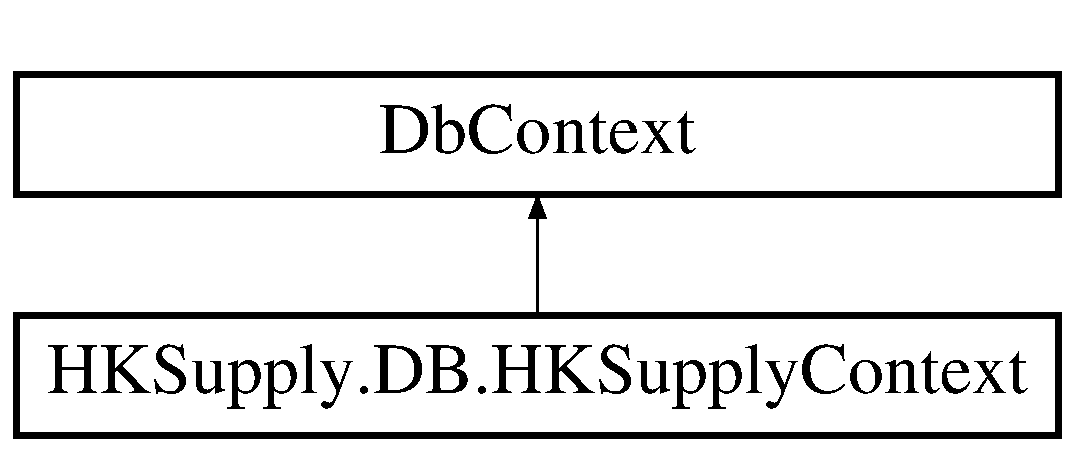
\includegraphics[height=2.000000cm]{class_h_k_supply_1_1_d_b_1_1_h_k_supply_context}
\end{center}
\end{figure}
\subsection*{Properties}
\begin{DoxyCompactItemize}
\item 
\mbox{\Hypertarget{class_h_k_supply_1_1_d_b_1_1_h_k_supply_context_aa13a9d69d5f081b45c75059370ae3201}\label{class_h_k_supply_1_1_d_b_1_1_h_k_supply_context_aa13a9d69d5f081b45c75059370ae3201}} 
Db\+Set$<$ \hyperlink{class_h_k_supply_1_1_models_1_1_role}{Role} $>$ {\bfseries Roles}\hspace{0.3cm}{\ttfamily  \mbox{[}get, set\mbox{]}}
\item 
\mbox{\Hypertarget{class_h_k_supply_1_1_d_b_1_1_h_k_supply_context_a2b7cfcd66fb7b707906ec3da46ee099f}\label{class_h_k_supply_1_1_d_b_1_1_h_k_supply_context_a2b7cfcd66fb7b707906ec3da46ee099f}} 
Db\+Set$<$ \hyperlink{class_h_k_supply_1_1_models_1_1_user}{User} $>$ {\bfseries Users}\hspace{0.3cm}{\ttfamily  \mbox{[}get, set\mbox{]}}
\item 
\mbox{\Hypertarget{class_h_k_supply_1_1_d_b_1_1_h_k_supply_context_a54ca6fe82e2574c81705e6b3686a1ce3}\label{class_h_k_supply_1_1_d_b_1_1_h_k_supply_context_a54ca6fe82e2574c81705e6b3686a1ce3}} 
Db\+Set$<$ \hyperlink{class_h_k_supply_1_1_models_1_1_functionality}{Functionality} $>$ {\bfseries Functionalities}\hspace{0.3cm}{\ttfamily  \mbox{[}get, set\mbox{]}}
\item 
\mbox{\Hypertarget{class_h_k_supply_1_1_d_b_1_1_h_k_supply_context_ad7edaaaf095a352171c4903fb774a482}\label{class_h_k_supply_1_1_d_b_1_1_h_k_supply_context_ad7edaaaf095a352171c4903fb774a482}} 
Db\+Set$<$ \hyperlink{class_h_k_supply_1_1_models_1_1_functionality_role}{Functionality\+Role} $>$ {\bfseries Functionalities\+Role}\hspace{0.3cm}{\ttfamily  \mbox{[}get, set\mbox{]}}
\item 
\mbox{\Hypertarget{class_h_k_supply_1_1_d_b_1_1_h_k_supply_context_a61798023df843c12bca882cb94bcda49}\label{class_h_k_supply_1_1_d_b_1_1_h_k_supply_context_a61798023df843c12bca882cb94bcda49}} 
Db\+Set$<$ \hyperlink{class_h_k_supply_1_1_models_1_1_customer}{Customer} $>$ {\bfseries Customers}\hspace{0.3cm}{\ttfamily  \mbox{[}get, set\mbox{]}}
\item 
\mbox{\Hypertarget{class_h_k_supply_1_1_d_b_1_1_h_k_supply_context_a07e9712da54d17365dcc738168829127}\label{class_h_k_supply_1_1_d_b_1_1_h_k_supply_context_a07e9712da54d17365dcc738168829127}} 
Db\+Set$<$ \hyperlink{class_h_k_supply_1_1_models_1_1_customer_history}{Customer\+History} $>$ {\bfseries Customers\+History}\hspace{0.3cm}{\ttfamily  \mbox{[}get, set\mbox{]}}
\end{DoxyCompactItemize}


\subsection{Detailed Description}
Contexto de base de datos Entity Framework 



The documentation for this class was generated from the following file\+:\begin{DoxyCompactItemize}
\item 
H\+K\+Supply/\+D\+B/H\+K\+Supply\+Context.\+cs\end{DoxyCompactItemize}

\hypertarget{interface_h_k_supply_1_1_services_1_1_interfaces_1_1_i_customer}{}\section{H\+K\+Supply.\+Services.\+Interfaces.\+I\+Customer Interface Reference}
\label{interface_h_k_supply_1_1_services_1_1_interfaces_1_1_i_customer}\index{H\+K\+Supply.\+Services.\+Interfaces.\+I\+Customer@{H\+K\+Supply.\+Services.\+Interfaces.\+I\+Customer}}
Inheritance diagram for H\+K\+Supply.\+Services.\+Interfaces.\+I\+Customer\+:\begin{figure}[H]
\begin{center}
\leavevmode
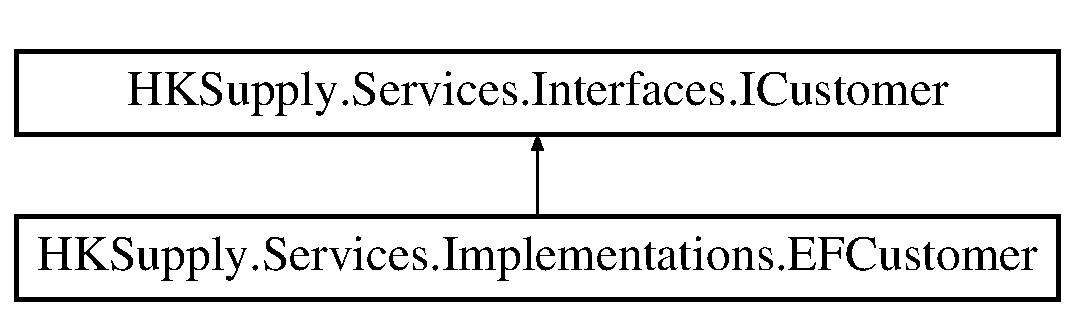
\includegraphics[height=2.000000cm]{interface_h_k_supply_1_1_services_1_1_interfaces_1_1_i_customer}
\end{center}
\end{figure}
\subsection*{Public Member Functions}
\begin{DoxyCompactItemize}
\item 
\mbox{\Hypertarget{interface_h_k_supply_1_1_services_1_1_interfaces_1_1_i_customer_a4eae770f8e05c2a16b30d11ca2b6a3e8}\label{interface_h_k_supply_1_1_services_1_1_interfaces_1_1_i_customer_a4eae770f8e05c2a16b30d11ca2b6a3e8}} 
bool {\bfseries New\+Customer} (\hyperlink{class_h_k_supply_1_1_models_1_1_customer}{Customer} new\+Customer)
\item 
\mbox{\Hypertarget{interface_h_k_supply_1_1_services_1_1_interfaces_1_1_i_customer_a2f446e665b10feef3e8373887a138048}\label{interface_h_k_supply_1_1_services_1_1_interfaces_1_1_i_customer_a2f446e665b10feef3e8373887a138048}} 
bool {\bfseries Update\+Customer} (\hyperlink{class_h_k_supply_1_1_models_1_1_customer}{Customer} update\+Customer, bool new\+Ver=false)
\item 
\mbox{\Hypertarget{interface_h_k_supply_1_1_services_1_1_interfaces_1_1_i_customer_a0ce0dce4e042cf94014fbc1487bf7789}\label{interface_h_k_supply_1_1_services_1_1_interfaces_1_1_i_customer_a0ce0dce4e042cf94014fbc1487bf7789}} 
\hyperlink{class_h_k_supply_1_1_models_1_1_customer}{Customer} {\bfseries Get\+Customer\+By\+Id} (string id\+Customer)
\end{DoxyCompactItemize}


The documentation for this interface was generated from the following file\+:\begin{DoxyCompactItemize}
\item 
H\+K\+Supply/\+Services/\+Interfaces/I\+Customer.\+cs\end{DoxyCompactItemize}

\hypertarget{interface_h_k_supply_1_1_services_1_1_interfaces_1_1_i_functionality}{}\section{H\+K\+Supply.\+Services.\+Interfaces.\+I\+Functionality Interface Reference}
\label{interface_h_k_supply_1_1_services_1_1_interfaces_1_1_i_functionality}\index{H\+K\+Supply.\+Services.\+Interfaces.\+I\+Functionality@{H\+K\+Supply.\+Services.\+Interfaces.\+I\+Functionality}}


Interface para el service de Functionality  


Inheritance diagram for H\+K\+Supply.\+Services.\+Interfaces.\+I\+Functionality\+:\begin{figure}[H]
\begin{center}
\leavevmode
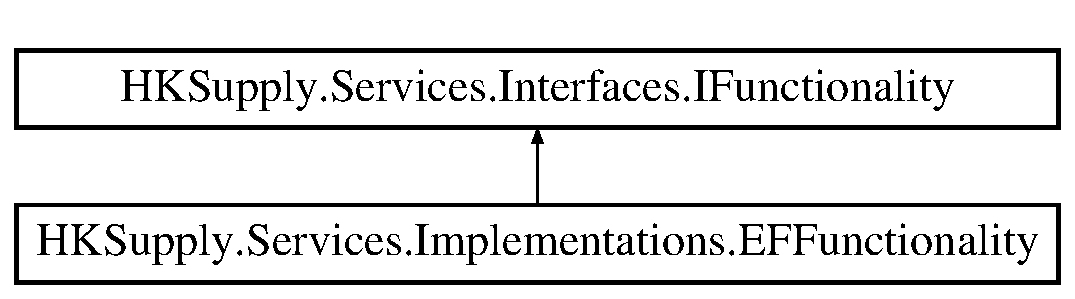
\includegraphics[height=2.000000cm]{interface_h_k_supply_1_1_services_1_1_interfaces_1_1_i_functionality}
\end{center}
\end{figure}
\subsection*{Public Member Functions}
\begin{DoxyCompactItemize}
\item 
\mbox{\Hypertarget{interface_h_k_supply_1_1_services_1_1_interfaces_1_1_i_functionality_aa1f16fee3ce5743db02605b4fd2184fc}\label{interface_h_k_supply_1_1_services_1_1_interfaces_1_1_i_functionality_aa1f16fee3ce5743db02605b4fd2184fc}} 
I\+Enumerable$<$ \hyperlink{class_h_k_supply_1_1_models_1_1_functionality}{Functionality} $>$ {\bfseries Get\+All\+Functionalities} ()
\item 
\mbox{\Hypertarget{interface_h_k_supply_1_1_services_1_1_interfaces_1_1_i_functionality_a7652aa4269664c60c38868ca5691b39e}\label{interface_h_k_supply_1_1_services_1_1_interfaces_1_1_i_functionality_a7652aa4269664c60c38868ca5691b39e}} 
\hyperlink{class_h_k_supply_1_1_models_1_1_functionality}{Functionality} {\bfseries Get\+Functionality\+By\+Id} (int functionality\+Id)
\item 
\mbox{\Hypertarget{interface_h_k_supply_1_1_services_1_1_interfaces_1_1_i_functionality_a8b71832d394e3900a477c05c346489df}\label{interface_h_k_supply_1_1_services_1_1_interfaces_1_1_i_functionality_a8b71832d394e3900a477c05c346489df}} 
\hyperlink{class_h_k_supply_1_1_models_1_1_functionality}{Functionality} {\bfseries Get\+Functionality\+By\+Name} (string functionality\+Name)
\item 
\mbox{\Hypertarget{interface_h_k_supply_1_1_services_1_1_interfaces_1_1_i_functionality_ac11ba1039efa6437e0669e9617ea5c9c}\label{interface_h_k_supply_1_1_services_1_1_interfaces_1_1_i_functionality_ac11ba1039efa6437e0669e9617ea5c9c}} 
\hyperlink{class_h_k_supply_1_1_models_1_1_functionality}{Functionality} {\bfseries New\+Functionality} (\hyperlink{class_h_k_supply_1_1_models_1_1_functionality}{Functionality} new\+Functionality)
\item 
\mbox{\Hypertarget{interface_h_k_supply_1_1_services_1_1_interfaces_1_1_i_functionality_a31203a06c78db03a2c9a69c0fa1a0865}\label{interface_h_k_supply_1_1_services_1_1_interfaces_1_1_i_functionality_a31203a06c78db03a2c9a69c0fa1a0865}} 
\hyperlink{class_h_k_supply_1_1_models_1_1_functionality}{Functionality} {\bfseries Modify\+Functionality} (\hyperlink{class_h_k_supply_1_1_models_1_1_functionality}{Functionality} mod\+Functionality)
\item 
\mbox{\Hypertarget{interface_h_k_supply_1_1_services_1_1_interfaces_1_1_i_functionality_a7408965d17ce5d8a6fea11ac392ed451}\label{interface_h_k_supply_1_1_services_1_1_interfaces_1_1_i_functionality_a7408965d17ce5d8a6fea11ac392ed451}} 
bool {\bfseries Update\+Functionalities} (I\+Enumerable$<$ \hyperlink{class_h_k_supply_1_1_models_1_1_functionality}{Functionality} $>$ functionalities\+To\+Update)
\end{DoxyCompactItemize}


\subsection{Detailed Description}
Interface para el service de Functionality 



The documentation for this interface was generated from the following file\+:\begin{DoxyCompactItemize}
\item 
H\+K\+Supply/\+Services/\+Interfaces/I\+Functionality.\+cs\end{DoxyCompactItemize}

\hypertarget{interface_h_k_supply_1_1_services_1_1_interfaces_1_1_i_functionality_role}{}\section{H\+K\+Supply.\+Services.\+Interfaces.\+I\+Functionality\+Role Interface Reference}
\label{interface_h_k_supply_1_1_services_1_1_interfaces_1_1_i_functionality_role}\index{H\+K\+Supply.\+Services.\+Interfaces.\+I\+Functionality\+Role@{H\+K\+Supply.\+Services.\+Interfaces.\+I\+Functionality\+Role}}


Interface para el service de Functionality -\/ Role  


Inheritance diagram for H\+K\+Supply.\+Services.\+Interfaces.\+I\+Functionality\+Role\+:\begin{figure}[H]
\begin{center}
\leavevmode
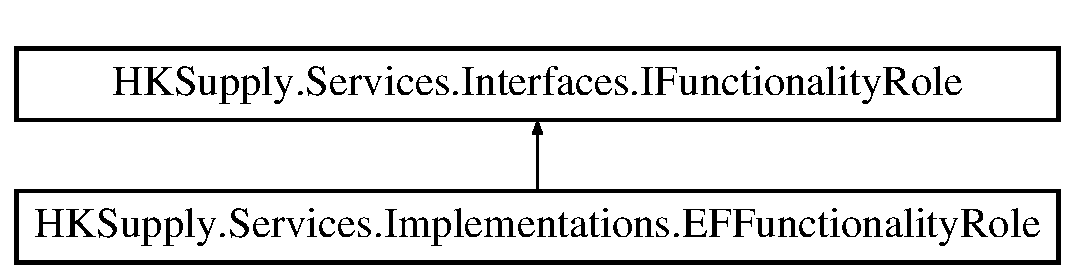
\includegraphics[height=2.000000cm]{interface_h_k_supply_1_1_services_1_1_interfaces_1_1_i_functionality_role}
\end{center}
\end{figure}
\subsection*{Public Member Functions}
\begin{DoxyCompactItemize}
\item 
\mbox{\Hypertarget{interface_h_k_supply_1_1_services_1_1_interfaces_1_1_i_functionality_role_a5db7b5d6e33c8f79666a34ab4460fcfd}\label{interface_h_k_supply_1_1_services_1_1_interfaces_1_1_i_functionality_role_a5db7b5d6e33c8f79666a34ab4460fcfd}} 
I\+Enumerable$<$ \mbox{\hyperlink{class_h_k_supply_1_1_models_1_1_functionality_role}{Functionality\+Role}} $>$ {\bfseries Get\+All\+Functionalities\+Role} ()
\item 
\mbox{\Hypertarget{interface_h_k_supply_1_1_services_1_1_interfaces_1_1_i_functionality_role_a10baae97837f0bffcbb4cd5e6d9da56d}\label{interface_h_k_supply_1_1_services_1_1_interfaces_1_1_i_functionality_role_a10baae97837f0bffcbb4cd5e6d9da56d}} 
\mbox{\hyperlink{class_h_k_supply_1_1_models_1_1_functionality_role}{Functionality\+Role}} {\bfseries Get\+Functionality\+Role} (int functionality\+Id, string role\+Id)
\item 
\mbox{\Hypertarget{interface_h_k_supply_1_1_services_1_1_interfaces_1_1_i_functionality_role_a75bfe6931c107903bfa876ca21eb032a}\label{interface_h_k_supply_1_1_services_1_1_interfaces_1_1_i_functionality_role_a75bfe6931c107903bfa876ca21eb032a}} 
I\+Enumerable$<$ \mbox{\hyperlink{class_h_k_supply_1_1_models_1_1_functionality_role}{Functionality\+Role}} $>$ {\bfseries Get\+Functionalities\+Role} (string role\+Id)
\item 
\mbox{\Hypertarget{interface_h_k_supply_1_1_services_1_1_interfaces_1_1_i_functionality_role_a9431314adb2c808619b1cde6366b68d7}\label{interface_h_k_supply_1_1_services_1_1_interfaces_1_1_i_functionality_role_a9431314adb2c808619b1cde6366b68d7}} 
I\+Enumerable$<$ string $>$ {\bfseries Get\+Functionalities\+Categories\+Role} (string role\+Id)
\item 
\mbox{\Hypertarget{interface_h_k_supply_1_1_services_1_1_interfaces_1_1_i_functionality_role_a8ccda5eb882dbe88c4d3f8257d6353b7}\label{interface_h_k_supply_1_1_services_1_1_interfaces_1_1_i_functionality_role_a8ccda5eb882dbe88c4d3f8257d6353b7}} 
\mbox{\hyperlink{class_h_k_supply_1_1_models_1_1_functionality_role}{Functionality\+Role}} {\bfseries New\+Functionality\+Role} (\mbox{\hyperlink{class_h_k_supply_1_1_models_1_1_functionality_role}{Functionality\+Role}} new\+Functionality\+Role)
\item 
\mbox{\Hypertarget{interface_h_k_supply_1_1_services_1_1_interfaces_1_1_i_functionality_role_af8f8d673b36ae48f98abfa43cfe59863}\label{interface_h_k_supply_1_1_services_1_1_interfaces_1_1_i_functionality_role_af8f8d673b36ae48f98abfa43cfe59863}} 
\mbox{\hyperlink{class_h_k_supply_1_1_models_1_1_functionality_role}{Functionality\+Role}} {\bfseries Modify\+Functionality\+Role} (\mbox{\hyperlink{class_h_k_supply_1_1_models_1_1_functionality_role}{Functionality\+Role}} mod\+Functionality\+Role)
\item 
\mbox{\Hypertarget{interface_h_k_supply_1_1_services_1_1_interfaces_1_1_i_functionality_role_a816ae3d8bb97d20aa19d3608d96528e5}\label{interface_h_k_supply_1_1_services_1_1_interfaces_1_1_i_functionality_role_a816ae3d8bb97d20aa19d3608d96528e5}} 
bool {\bfseries Update\+Functionalities\+Roles} (I\+Enumerable$<$ \mbox{\hyperlink{class_h_k_supply_1_1_models_1_1_functionality_role}{Functionality\+Role}} $>$ functionalities\+Roles\+To\+Update)
\end{DoxyCompactItemize}


\subsection{Detailed Description}
Interface para el service de Functionality -\/ Role 



The documentation for this interface was generated from the following file\+:\begin{DoxyCompactItemize}
\item 
H\+K\+Supply/\+Services/\+Interfaces/I\+Functionality\+Role.\+cs\end{DoxyCompactItemize}

\hypertarget{class_h_k_supply_1_1_exceptions_1_1_invalid_password_exception}{}\section{H\+K\+Supply.\+Exceptions.\+Invalid\+Password\+Exception Class Reference}
\label{class_h_k_supply_1_1_exceptions_1_1_invalid_password_exception}\index{H\+K\+Supply.\+Exceptions.\+Invalid\+Password\+Exception@{H\+K\+Supply.\+Exceptions.\+Invalid\+Password\+Exception}}


Custom Exception para una contraseña incorrecta  


Inheritance diagram for H\+K\+Supply.\+Exceptions.\+Invalid\+Password\+Exception\+:\begin{figure}[H]
\begin{center}
\leavevmode
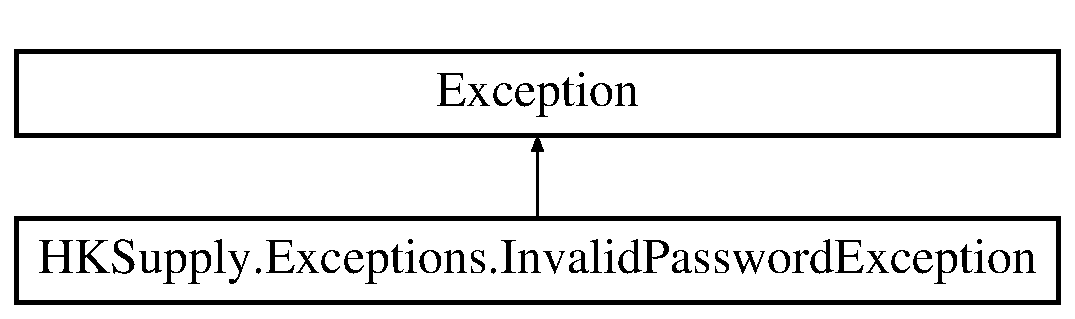
\includegraphics[height=2.000000cm]{class_h_k_supply_1_1_exceptions_1_1_invalid_password_exception}
\end{center}
\end{figure}
\subsection*{Public Member Functions}
\begin{DoxyCompactItemize}
\item 
\mbox{\Hypertarget{class_h_k_supply_1_1_exceptions_1_1_invalid_password_exception_aa25a42b91b39d8b234196368cc92f1be}\label{class_h_k_supply_1_1_exceptions_1_1_invalid_password_exception_aa25a42b91b39d8b234196368cc92f1be}} 
{\bfseries Invalid\+Password\+Exception} (string message)
\item 
\mbox{\Hypertarget{class_h_k_supply_1_1_exceptions_1_1_invalid_password_exception_a5179c29723f14deef7f1d26eea1e7f3f}\label{class_h_k_supply_1_1_exceptions_1_1_invalid_password_exception_a5179c29723f14deef7f1d26eea1e7f3f}} 
{\bfseries Invalid\+Password\+Exception} (string message, System.\+Exception inner)
\end{DoxyCompactItemize}
\subsection*{Protected Member Functions}
\begin{DoxyCompactItemize}
\item 
\mbox{\Hypertarget{class_h_k_supply_1_1_exceptions_1_1_invalid_password_exception_a017a6b8ebe5e4db12eee08b0feb75edc}\label{class_h_k_supply_1_1_exceptions_1_1_invalid_password_exception_a017a6b8ebe5e4db12eee08b0feb75edc}} 
{\bfseries Invalid\+Password\+Exception} (System.\+Runtime.\+Serialization.\+Serialization\+Info info, System.\+Runtime.\+Serialization.\+Streaming\+Context context)
\end{DoxyCompactItemize}


\subsection{Detailed Description}
Custom Exception para una contraseña incorrecta 



The documentation for this class was generated from the following file\+:\begin{DoxyCompactItemize}
\item 
H\+K\+Supply/\+Exceptions/Invalid\+Password\+Exception.\+cs\end{DoxyCompactItemize}

\hypertarget{interface_h_k_supply_1_1_services_1_1_interfaces_1_1_i_role}{}\section{H\+K\+Supply.\+Services.\+Interfaces.\+I\+Role Interface Reference}
\label{interface_h_k_supply_1_1_services_1_1_interfaces_1_1_i_role}\index{H\+K\+Supply.\+Services.\+Interfaces.\+I\+Role@{H\+K\+Supply.\+Services.\+Interfaces.\+I\+Role}}


Interface para el service de Role  


Inheritance diagram for H\+K\+Supply.\+Services.\+Interfaces.\+I\+Role\+:\begin{figure}[H]
\begin{center}
\leavevmode
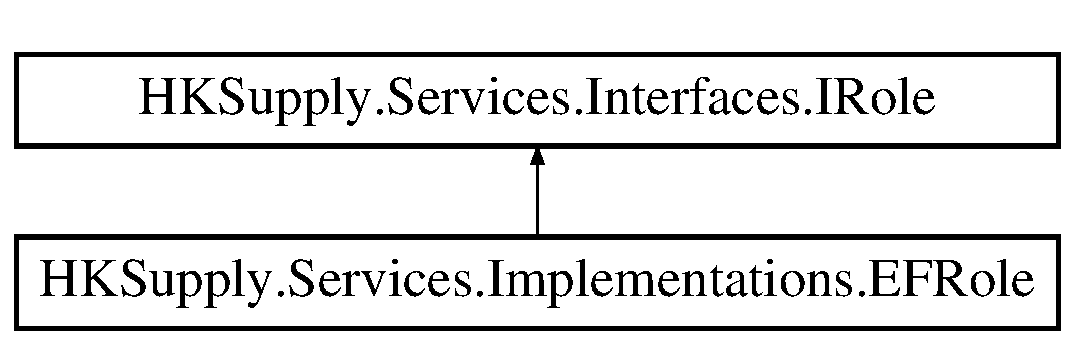
\includegraphics[height=2.000000cm]{interface_h_k_supply_1_1_services_1_1_interfaces_1_1_i_role}
\end{center}
\end{figure}
\subsection*{Public Member Functions}
\begin{DoxyCompactItemize}
\item 
\mbox{\Hypertarget{interface_h_k_supply_1_1_services_1_1_interfaces_1_1_i_role_a921bacd80020de3cf811705857c9eb7e}\label{interface_h_k_supply_1_1_services_1_1_interfaces_1_1_i_role_a921bacd80020de3cf811705857c9eb7e}} 
I\+Enumerable$<$ \mbox{\hyperlink{class_h_k_supply_1_1_models_1_1_role}{Role}} $>$ {\bfseries Get\+Roles} (bool all=true)
\item 
\mbox{\Hypertarget{interface_h_k_supply_1_1_services_1_1_interfaces_1_1_i_role_ad83423359435ae70026a1daac5bd07ae}\label{interface_h_k_supply_1_1_services_1_1_interfaces_1_1_i_role_ad83423359435ae70026a1daac5bd07ae}} 
\mbox{\hyperlink{class_h_k_supply_1_1_models_1_1_role}{Role}} {\bfseries Get\+Role\+By\+Id} (string role\+Id)
\item 
\mbox{\Hypertarget{interface_h_k_supply_1_1_services_1_1_interfaces_1_1_i_role_a7fea1e910bcd64d8e99da8bf4438e50f}\label{interface_h_k_supply_1_1_services_1_1_interfaces_1_1_i_role_a7fea1e910bcd64d8e99da8bf4438e50f}} 
\mbox{\hyperlink{class_h_k_supply_1_1_models_1_1_role}{Role}} {\bfseries New\+Role} (\mbox{\hyperlink{class_h_k_supply_1_1_models_1_1_role}{Role}} new\+Role)
\item 
\mbox{\Hypertarget{interface_h_k_supply_1_1_services_1_1_interfaces_1_1_i_role_a4f5e4bf501b1affbae4d3d39dbb837b5}\label{interface_h_k_supply_1_1_services_1_1_interfaces_1_1_i_role_a4f5e4bf501b1affbae4d3d39dbb837b5}} 
bool {\bfseries Disable\+Role} (string role\+Id, string remarks)
\item 
\mbox{\Hypertarget{interface_h_k_supply_1_1_services_1_1_interfaces_1_1_i_role_a0960468c3fb4db4f09b3175106ee7753}\label{interface_h_k_supply_1_1_services_1_1_interfaces_1_1_i_role_a0960468c3fb4db4f09b3175106ee7753}} 
bool {\bfseries Update\+Roles} (I\+Enumerable$<$ \mbox{\hyperlink{class_h_k_supply_1_1_models_1_1_role}{Role}} $>$ roles\+To\+Update)
\end{DoxyCompactItemize}


\subsection{Detailed Description}
Interface para el service de Role 



The documentation for this interface was generated from the following file\+:\begin{DoxyCompactItemize}
\item 
H\+K\+Supply/\+Services/\+Interfaces/I\+Role.\+cs\end{DoxyCompactItemize}

\hypertarget{interface_h_k_supply_1_1_services_1_1_interfaces_1_1_i_user}{}\section{H\+K\+Supply.\+Services.\+Interfaces.\+I\+User Interface Reference}
\label{interface_h_k_supply_1_1_services_1_1_interfaces_1_1_i_user}\index{H\+K\+Supply.\+Services.\+Interfaces.\+I\+User@{H\+K\+Supply.\+Services.\+Interfaces.\+I\+User}}


Interface para el service de User  


Inheritance diagram for H\+K\+Supply.\+Services.\+Interfaces.\+I\+User\+:\begin{figure}[H]
\begin{center}
\leavevmode
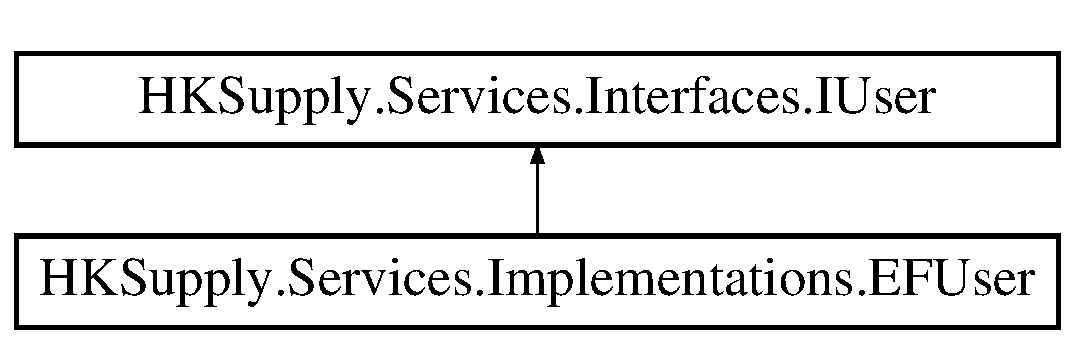
\includegraphics[height=2.000000cm]{interface_h_k_supply_1_1_services_1_1_interfaces_1_1_i_user}
\end{center}
\end{figure}
\subsection*{Public Member Functions}
\begin{DoxyCompactItemize}
\item 
\mbox{\Hypertarget{interface_h_k_supply_1_1_services_1_1_interfaces_1_1_i_user_ab18e28f31a3a14a63df31f17991aeb43}\label{interface_h_k_supply_1_1_services_1_1_interfaces_1_1_i_user_ab18e28f31a3a14a63df31f17991aeb43}} 
I\+Enumerable$<$ \hyperlink{class_h_k_supply_1_1_models_1_1_user}{User} $>$ {\bfseries Get\+All\+Users} ()
\item 
\mbox{\Hypertarget{interface_h_k_supply_1_1_services_1_1_interfaces_1_1_i_user_a49a1d525d5ab93f26cbe66b1f22abe1a}\label{interface_h_k_supply_1_1_services_1_1_interfaces_1_1_i_user_a49a1d525d5ab93f26cbe66b1f22abe1a}} 
\hyperlink{class_h_k_supply_1_1_models_1_1_user}{User} {\bfseries Get\+User\+By\+Id} (int user\+Id)
\item 
\mbox{\Hypertarget{interface_h_k_supply_1_1_services_1_1_interfaces_1_1_i_user_a814c835f9375a134f01ad961e27d7314}\label{interface_h_k_supply_1_1_services_1_1_interfaces_1_1_i_user_a814c835f9375a134f01ad961e27d7314}} 
\hyperlink{class_h_k_supply_1_1_models_1_1_user}{User} {\bfseries Get\+User\+By\+Login\+Password} (string User\+Login, string Password)
\item 
\mbox{\Hypertarget{interface_h_k_supply_1_1_services_1_1_interfaces_1_1_i_user_a0f68a7ca2668977e45d199ea21522a98}\label{interface_h_k_supply_1_1_services_1_1_interfaces_1_1_i_user_a0f68a7ca2668977e45d199ea21522a98}} 
\hyperlink{class_h_k_supply_1_1_models_1_1_user}{User} {\bfseries New\+User} (\hyperlink{class_h_k_supply_1_1_models_1_1_user}{User} new\+User)
\item 
\mbox{\Hypertarget{interface_h_k_supply_1_1_services_1_1_interfaces_1_1_i_user_af241b1a787265f454b2d5b33a8514ff0}\label{interface_h_k_supply_1_1_services_1_1_interfaces_1_1_i_user_af241b1a787265f454b2d5b33a8514ff0}} 
bool {\bfseries Disable\+User} (string user\+Id, string remarks)
\item 
\mbox{\Hypertarget{interface_h_k_supply_1_1_services_1_1_interfaces_1_1_i_user_a437f1837393b7a306de3fecdce176c97}\label{interface_h_k_supply_1_1_services_1_1_interfaces_1_1_i_user_a437f1837393b7a306de3fecdce176c97}} 
bool {\bfseries Change\+Password} (int user\+Id, string password)
\item 
\mbox{\Hypertarget{interface_h_k_supply_1_1_services_1_1_interfaces_1_1_i_user_a61282883d17b0cf41a07a93e9bd49db7}\label{interface_h_k_supply_1_1_services_1_1_interfaces_1_1_i_user_a61282883d17b0cf41a07a93e9bd49db7}} 
bool {\bfseries Update\+Users} (I\+Enumerable$<$ \hyperlink{class_h_k_supply_1_1_models_1_1_user}{User} $>$ users\+To\+Update)
\end{DoxyCompactItemize}


\subsection{Detailed Description}
Interface para el service de User 



The documentation for this interface was generated from the following file\+:\begin{DoxyCompactItemize}
\item 
H\+K\+Supply/\+Services/\+Interfaces/I\+User.\+cs\end{DoxyCompactItemize}

\hypertarget{class_h_k_supply_1_1_forms_1_1_login}{}\section{H\+K\+Supply.\+Forms.\+Login Class Reference}
\label{class_h_k_supply_1_1_forms_1_1_login}\index{H\+K\+Supply.\+Forms.\+Login@{H\+K\+Supply.\+Forms.\+Login}}
Inheritance diagram for H\+K\+Supply.\+Forms.\+Login\+:\begin{figure}[H]
\begin{center}
\leavevmode
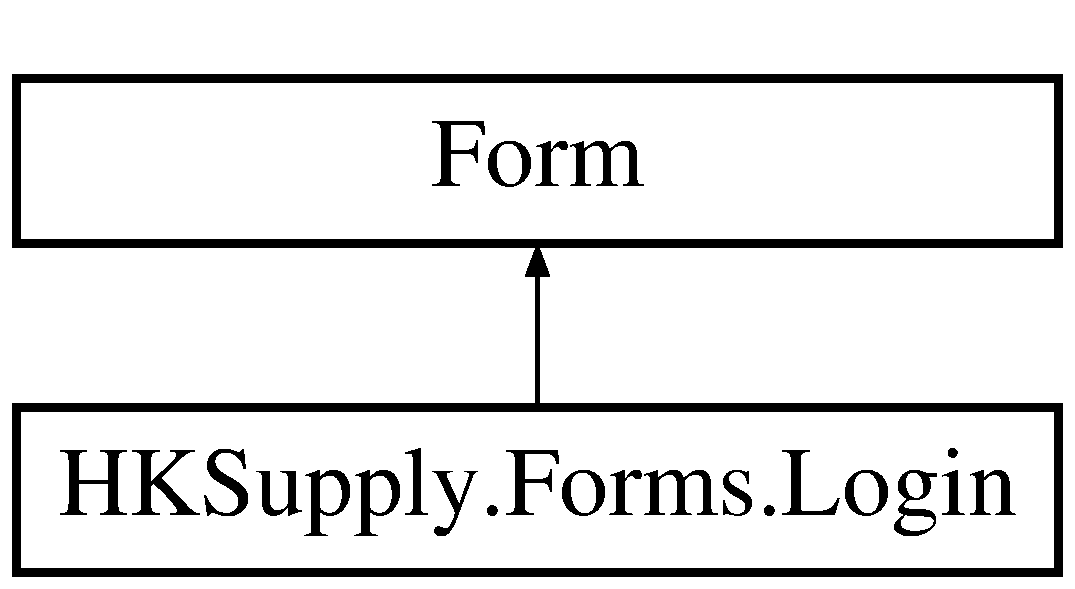
\includegraphics[height=2.000000cm]{class_h_k_supply_1_1_forms_1_1_login}
\end{center}
\end{figure}
\subsection*{Protected Member Functions}
\begin{DoxyCompactItemize}
\item 
override void \mbox{\hyperlink{class_h_k_supply_1_1_forms_1_1_login_a0c20fcbe198d2635836e7c7c6eebee31}{Dispose}} (bool disposing)
\begin{DoxyCompactList}\small\item\em Clean up any resources being used. \end{DoxyCompactList}\end{DoxyCompactItemize}


\subsection{Member Function Documentation}
\mbox{\Hypertarget{class_h_k_supply_1_1_forms_1_1_login_a0c20fcbe198d2635836e7c7c6eebee31}\label{class_h_k_supply_1_1_forms_1_1_login_a0c20fcbe198d2635836e7c7c6eebee31}} 
\index{H\+K\+Supply\+::\+Forms\+::\+Login@{H\+K\+Supply\+::\+Forms\+::\+Login}!Dispose@{Dispose}}
\index{Dispose@{Dispose}!H\+K\+Supply\+::\+Forms\+::\+Login@{H\+K\+Supply\+::\+Forms\+::\+Login}}
\subsubsection{\texorpdfstring{Dispose()}{Dispose()}}
{\footnotesize\ttfamily override void H\+K\+Supply.\+Forms.\+Login.\+Dispose (\begin{DoxyParamCaption}\item[{bool}]{disposing }\end{DoxyParamCaption})\hspace{0.3cm}{\ttfamily [protected]}}



Clean up any resources being used. 


\begin{DoxyParams}{Parameters}
{\em disposing} & true if managed resources should be disposed; otherwise, false.\\
\hline
\end{DoxyParams}


The documentation for this class was generated from the following files\+:\begin{DoxyCompactItemize}
\item 
H\+K\+Supply/\+Forms/Login.\+cs\item 
H\+K\+Supply/\+Forms/Login.\+Designer.\+cs\end{DoxyCompactItemize}

\hypertarget{class_h_k_supply_1_1_forms_1_1_main}{}\section{H\+K\+Supply.\+Forms.\+Main Class Reference}
\label{class_h_k_supply_1_1_forms_1_1_main}\index{H\+K\+Supply.\+Forms.\+Main@{H\+K\+Supply.\+Forms.\+Main}}
Inheritance diagram for H\+K\+Supply.\+Forms.\+Main\+:\begin{figure}[H]
\begin{center}
\leavevmode
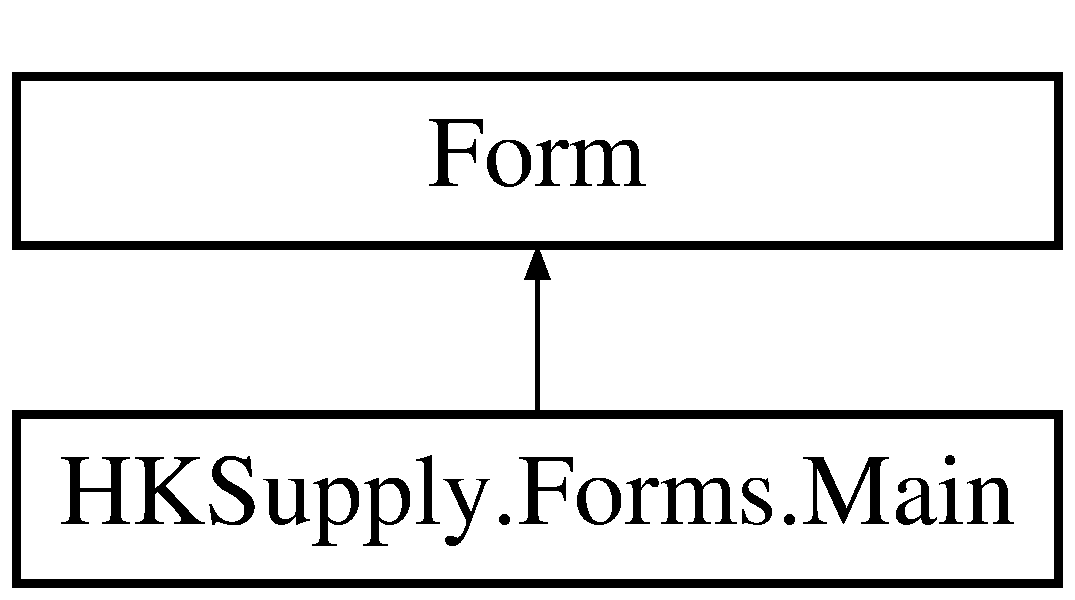
\includegraphics[height=2.000000cm]{class_h_k_supply_1_1_forms_1_1_main}
\end{center}
\end{figure}
\subsection*{Public Member Functions}
\begin{DoxyCompactItemize}
\item 
\mbox{\Hypertarget{class_h_k_supply_1_1_forms_1_1_main_ae322c78605a4993241d8cf837cc2e6fc}\label{class_h_k_supply_1_1_forms_1_1_main_ae322c78605a4993241d8cf837cc2e6fc}} 
void {\bfseries Child\+Click} (object sender, System.\+Event\+Args e)
\item 
\mbox{\Hypertarget{class_h_k_supply_1_1_forms_1_1_main_addabcc6880d05211cf957130edb2bbe3}\label{class_h_k_supply_1_1_forms_1_1_main_addabcc6880d05211cf957130edb2bbe3}} 
void {\bfseries Child\+Pdf\+Click} (object sender, System.\+Event\+Args e)
\end{DoxyCompactItemize}
\subsection*{Protected Member Functions}
\begin{DoxyCompactItemize}
\item 
override void \mbox{\hyperlink{class_h_k_supply_1_1_forms_1_1_main_a99fe43d79c789818b37bb46db1dfa795}{Dispose}} (bool disposing)
\begin{DoxyCompactList}\small\item\em Clean up any resources being used. \end{DoxyCompactList}\end{DoxyCompactItemize}


\subsection{Member Function Documentation}
\mbox{\Hypertarget{class_h_k_supply_1_1_forms_1_1_main_a99fe43d79c789818b37bb46db1dfa795}\label{class_h_k_supply_1_1_forms_1_1_main_a99fe43d79c789818b37bb46db1dfa795}} 
\index{H\+K\+Supply\+::\+Forms\+::\+Main@{H\+K\+Supply\+::\+Forms\+::\+Main}!Dispose@{Dispose}}
\index{Dispose@{Dispose}!H\+K\+Supply\+::\+Forms\+::\+Main@{H\+K\+Supply\+::\+Forms\+::\+Main}}
\subsubsection{\texorpdfstring{Dispose()}{Dispose()}}
{\footnotesize\ttfamily override void H\+K\+Supply.\+Forms.\+Main.\+Dispose (\begin{DoxyParamCaption}\item[{bool}]{disposing }\end{DoxyParamCaption})\hspace{0.3cm}{\ttfamily [protected]}}



Clean up any resources being used. 


\begin{DoxyParams}{Parameters}
{\em disposing} & true if managed resources should be disposed; otherwise, false.\\
\hline
\end{DoxyParams}


The documentation for this class was generated from the following files\+:\begin{DoxyCompactItemize}
\item 
H\+K\+Supply/\+Forms/Main.\+cs\item 
H\+K\+Supply/\+Forms/Main.\+Designer.\+cs\end{DoxyCompactItemize}

\hypertarget{class_h_k_supply_1_1_exceptions_1_1_new_existing_functionality_exception}{}\section{H\+K\+Supply.\+Exceptions.\+New\+Existing\+Functionality\+Exception Class Reference}
\label{class_h_k_supply_1_1_exceptions_1_1_new_existing_functionality_exception}\index{H\+K\+Supply.\+Exceptions.\+New\+Existing\+Functionality\+Exception@{H\+K\+Supply.\+Exceptions.\+New\+Existing\+Functionality\+Exception}}


Custom Exception\+: dar de alta una funcionalidad ya existente en el sistema  


Inheritance diagram for H\+K\+Supply.\+Exceptions.\+New\+Existing\+Functionality\+Exception\+:\begin{figure}[H]
\begin{center}
\leavevmode
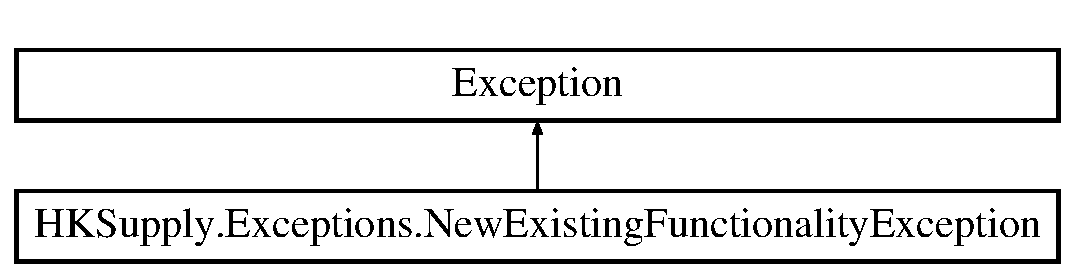
\includegraphics[height=2.000000cm]{class_h_k_supply_1_1_exceptions_1_1_new_existing_functionality_exception}
\end{center}
\end{figure}
\subsection*{Public Member Functions}
\begin{DoxyCompactItemize}
\item 
\mbox{\Hypertarget{class_h_k_supply_1_1_exceptions_1_1_new_existing_functionality_exception_a955fdbac911227d08700761322d1caf4}\label{class_h_k_supply_1_1_exceptions_1_1_new_existing_functionality_exception_a955fdbac911227d08700761322d1caf4}} 
{\bfseries New\+Existing\+Functionality\+Exception} (string message)
\item 
\mbox{\Hypertarget{class_h_k_supply_1_1_exceptions_1_1_new_existing_functionality_exception_ad618069f35b77e231be47075550f3532}\label{class_h_k_supply_1_1_exceptions_1_1_new_existing_functionality_exception_ad618069f35b77e231be47075550f3532}} 
{\bfseries New\+Existing\+Functionality\+Exception} (string message, System.\+Exception inner)
\end{DoxyCompactItemize}
\subsection*{Protected Member Functions}
\begin{DoxyCompactItemize}
\item 
\mbox{\Hypertarget{class_h_k_supply_1_1_exceptions_1_1_new_existing_functionality_exception_aab365582c771361d35fdf7bda9cd0c11}\label{class_h_k_supply_1_1_exceptions_1_1_new_existing_functionality_exception_aab365582c771361d35fdf7bda9cd0c11}} 
{\bfseries New\+Existing\+Functionality\+Exception} (System.\+Runtime.\+Serialization.\+Serialization\+Info info, System.\+Runtime.\+Serialization.\+Streaming\+Context context)
\end{DoxyCompactItemize}


\subsection{Detailed Description}
Custom Exception\+: dar de alta una funcionalidad ya existente en el sistema 



The documentation for this class was generated from the following file\+:\begin{DoxyCompactItemize}
\item 
H\+K\+Supply/\+Exceptions/New\+Existing\+Functionality\+Exception.\+cs\end{DoxyCompactItemize}

\hypertarget{class_h_k_supply_1_1_exceptions_1_1_new_existing_functionality_role_exception}{}\section{H\+K\+Supply.\+Exceptions.\+New\+Existing\+Functionality\+Role\+Exception Class Reference}
\label{class_h_k_supply_1_1_exceptions_1_1_new_existing_functionality_role_exception}\index{H\+K\+Supply.\+Exceptions.\+New\+Existing\+Functionality\+Role\+Exception@{H\+K\+Supply.\+Exceptions.\+New\+Existing\+Functionality\+Role\+Exception}}


Custom Exception\+: dar de alta una funcionalidad-\/role ya existente en el sistema  


Inheritance diagram for H\+K\+Supply.\+Exceptions.\+New\+Existing\+Functionality\+Role\+Exception\+:\begin{figure}[H]
\begin{center}
\leavevmode
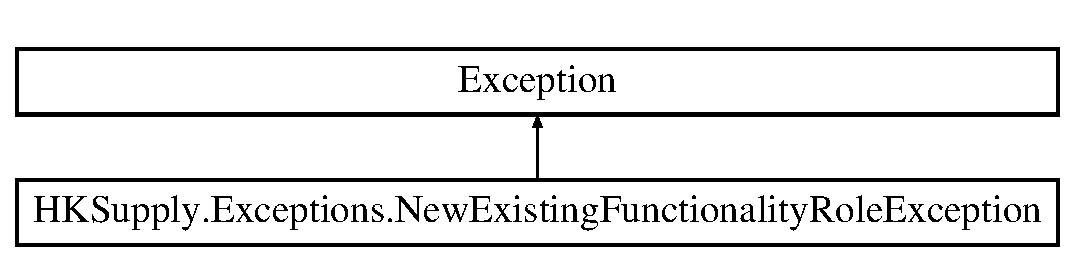
\includegraphics[height=2.000000cm]{class_h_k_supply_1_1_exceptions_1_1_new_existing_functionality_role_exception}
\end{center}
\end{figure}
\subsection*{Public Member Functions}
\begin{DoxyCompactItemize}
\item 
\mbox{\Hypertarget{class_h_k_supply_1_1_exceptions_1_1_new_existing_functionality_role_exception_ae1ed7abcf4a622331f3e876b9ca2e37a}\label{class_h_k_supply_1_1_exceptions_1_1_new_existing_functionality_role_exception_ae1ed7abcf4a622331f3e876b9ca2e37a}} 
{\bfseries New\+Existing\+Functionality\+Role\+Exception} (string message)
\item 
\mbox{\Hypertarget{class_h_k_supply_1_1_exceptions_1_1_new_existing_functionality_role_exception_a2ee1d1ca9bde3637d664788761bf090d}\label{class_h_k_supply_1_1_exceptions_1_1_new_existing_functionality_role_exception_a2ee1d1ca9bde3637d664788761bf090d}} 
{\bfseries New\+Existing\+Functionality\+Role\+Exception} (string message, System.\+Exception inner)
\end{DoxyCompactItemize}
\subsection*{Protected Member Functions}
\begin{DoxyCompactItemize}
\item 
\mbox{\Hypertarget{class_h_k_supply_1_1_exceptions_1_1_new_existing_functionality_role_exception_aa5ab783d50373a4cc5e74bdb0d69a169}\label{class_h_k_supply_1_1_exceptions_1_1_new_existing_functionality_role_exception_aa5ab783d50373a4cc5e74bdb0d69a169}} 
{\bfseries New\+Existing\+Functionality\+Role\+Exception} (System.\+Runtime.\+Serialization.\+Serialization\+Info info, System.\+Runtime.\+Serialization.\+Streaming\+Context context)
\end{DoxyCompactItemize}


\subsection{Detailed Description}
Custom Exception\+: dar de alta una funcionalidad-\/role ya existente en el sistema 



The documentation for this class was generated from the following file\+:\begin{DoxyCompactItemize}
\item 
H\+K\+Supply/\+Exceptions/New\+Existing\+Functionality\+Role\+Exception.\+cs\end{DoxyCompactItemize}

\hypertarget{class_h_k_supply_1_1_exceptions_1_1_new_existing_role_exception}{}\section{H\+K\+Supply.\+Exceptions.\+New\+Existing\+Role\+Exception Class Reference}
\label{class_h_k_supply_1_1_exceptions_1_1_new_existing_role_exception}\index{H\+K\+Supply.\+Exceptions.\+New\+Existing\+Role\+Exception@{H\+K\+Supply.\+Exceptions.\+New\+Existing\+Role\+Exception}}


Custom Exception\+: dar de alta un rol ya existente en el sistema  


Inheritance diagram for H\+K\+Supply.\+Exceptions.\+New\+Existing\+Role\+Exception\+:\begin{figure}[H]
\begin{center}
\leavevmode
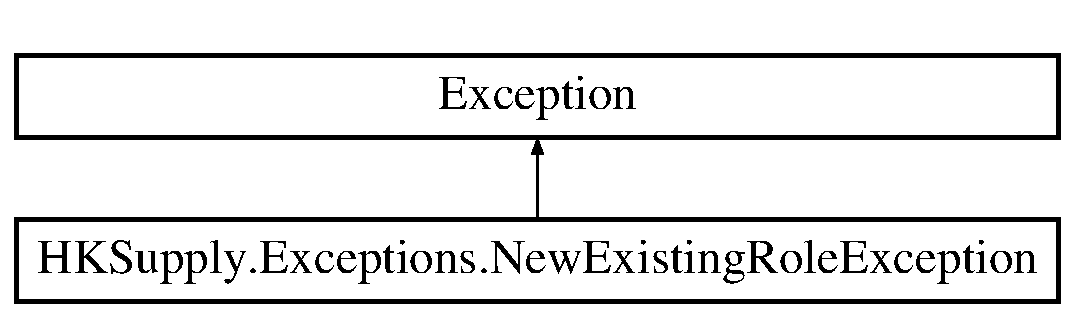
\includegraphics[height=2.000000cm]{class_h_k_supply_1_1_exceptions_1_1_new_existing_role_exception}
\end{center}
\end{figure}
\subsection*{Public Member Functions}
\begin{DoxyCompactItemize}
\item 
\mbox{\Hypertarget{class_h_k_supply_1_1_exceptions_1_1_new_existing_role_exception_a3a48fc075f0377064ce7394fd9123f2e}\label{class_h_k_supply_1_1_exceptions_1_1_new_existing_role_exception_a3a48fc075f0377064ce7394fd9123f2e}} 
{\bfseries New\+Existing\+Role\+Exception} (string message)
\item 
\mbox{\Hypertarget{class_h_k_supply_1_1_exceptions_1_1_new_existing_role_exception_a5d31e75345337147a74a40e9b2d657b6}\label{class_h_k_supply_1_1_exceptions_1_1_new_existing_role_exception_a5d31e75345337147a74a40e9b2d657b6}} 
{\bfseries New\+Existing\+Role\+Exception} (string message, System.\+Exception inner)
\end{DoxyCompactItemize}
\subsection*{Protected Member Functions}
\begin{DoxyCompactItemize}
\item 
\mbox{\Hypertarget{class_h_k_supply_1_1_exceptions_1_1_new_existing_role_exception_ae2c332b45921778b7d21a4915135b29a}\label{class_h_k_supply_1_1_exceptions_1_1_new_existing_role_exception_ae2c332b45921778b7d21a4915135b29a}} 
{\bfseries New\+Existing\+Role\+Exception} (System.\+Runtime.\+Serialization.\+Serialization\+Info info, System.\+Runtime.\+Serialization.\+Streaming\+Context context)
\end{DoxyCompactItemize}


\subsection{Detailed Description}
Custom Exception\+: dar de alta un rol ya existente en el sistema 



The documentation for this class was generated from the following file\+:\begin{DoxyCompactItemize}
\item 
H\+K\+Supply/\+Exceptions/New\+Existing\+Role\+Exception.\+cs\end{DoxyCompactItemize}

\hypertarget{class_h_k_supply_1_1_exceptions_1_1_new_existing_user_exception}{}\section{H\+K\+Supply.\+Exceptions.\+New\+Existing\+User\+Exception Class Reference}
\label{class_h_k_supply_1_1_exceptions_1_1_new_existing_user_exception}\index{H\+K\+Supply.\+Exceptions.\+New\+Existing\+User\+Exception@{H\+K\+Supply.\+Exceptions.\+New\+Existing\+User\+Exception}}


Custom Exception\+: dar de alta un usuario ya existente en el sistema  


Inheritance diagram for H\+K\+Supply.\+Exceptions.\+New\+Existing\+User\+Exception\+:\begin{figure}[H]
\begin{center}
\leavevmode
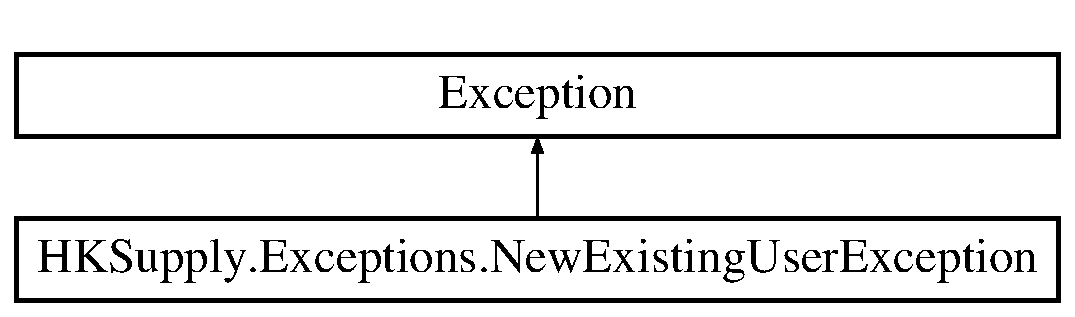
\includegraphics[height=2.000000cm]{class_h_k_supply_1_1_exceptions_1_1_new_existing_user_exception}
\end{center}
\end{figure}
\subsection*{Public Member Functions}
\begin{DoxyCompactItemize}
\item 
\mbox{\Hypertarget{class_h_k_supply_1_1_exceptions_1_1_new_existing_user_exception_ab2021ca5058ce5ace749b56519f6fdab}\label{class_h_k_supply_1_1_exceptions_1_1_new_existing_user_exception_ab2021ca5058ce5ace749b56519f6fdab}} 
{\bfseries New\+Existing\+User\+Exception} (string message)
\item 
\mbox{\Hypertarget{class_h_k_supply_1_1_exceptions_1_1_new_existing_user_exception_a8514fcb25cba282c24871071d9eb28bb}\label{class_h_k_supply_1_1_exceptions_1_1_new_existing_user_exception_a8514fcb25cba282c24871071d9eb28bb}} 
{\bfseries New\+Existing\+User\+Exception} (string message, System.\+Exception inner)
\end{DoxyCompactItemize}
\subsection*{Protected Member Functions}
\begin{DoxyCompactItemize}
\item 
\mbox{\Hypertarget{class_h_k_supply_1_1_exceptions_1_1_new_existing_user_exception_a12b02cfddf08f6c91fdff4bad9c0e65b}\label{class_h_k_supply_1_1_exceptions_1_1_new_existing_user_exception_a12b02cfddf08f6c91fdff4bad9c0e65b}} 
{\bfseries New\+Existing\+User\+Exception} (System.\+Runtime.\+Serialization.\+Serialization\+Info info, System.\+Runtime.\+Serialization.\+Streaming\+Context context)
\end{DoxyCompactItemize}


\subsection{Detailed Description}
Custom Exception\+: dar de alta un usuario ya existente en el sistema 



The documentation for this class was generated from the following file\+:\begin{DoxyCompactItemize}
\item 
H\+K\+Supply/\+Exceptions/New\+Existing\+User\+Exception.\+cs\end{DoxyCompactItemize}

\hypertarget{class_h_k_supply_1_1_exceptions_1_1_nonexistent_functionality_exception}{}\section{H\+K\+Supply.\+Exceptions.\+Nonexistent\+Functionality\+Exception Class Reference}
\label{class_h_k_supply_1_1_exceptions_1_1_nonexistent_functionality_exception}\index{H\+K\+Supply.\+Exceptions.\+Nonexistent\+Functionality\+Exception@{H\+K\+Supply.\+Exceptions.\+Nonexistent\+Functionality\+Exception}}


Custom Exception\+: funcionalidad no existente en el sistema  


Inheritance diagram for H\+K\+Supply.\+Exceptions.\+Nonexistent\+Functionality\+Exception\+:\begin{figure}[H]
\begin{center}
\leavevmode
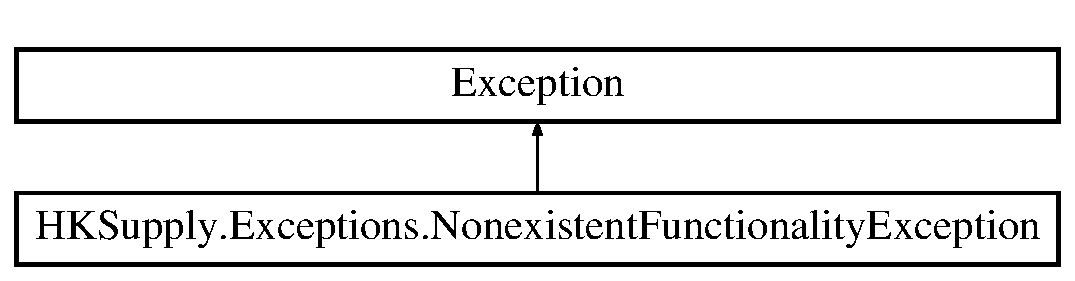
\includegraphics[height=2.000000cm]{class_h_k_supply_1_1_exceptions_1_1_nonexistent_functionality_exception}
\end{center}
\end{figure}
\subsection*{Public Member Functions}
\begin{DoxyCompactItemize}
\item 
\mbox{\Hypertarget{class_h_k_supply_1_1_exceptions_1_1_nonexistent_functionality_exception_a401756b880c4a3750896f980b505bc8c}\label{class_h_k_supply_1_1_exceptions_1_1_nonexistent_functionality_exception_a401756b880c4a3750896f980b505bc8c}} 
{\bfseries Nonexistent\+Functionality\+Exception} (string message)
\item 
\mbox{\Hypertarget{class_h_k_supply_1_1_exceptions_1_1_nonexistent_functionality_exception_aa5e5ab000237411d1b13343128650cda}\label{class_h_k_supply_1_1_exceptions_1_1_nonexistent_functionality_exception_aa5e5ab000237411d1b13343128650cda}} 
{\bfseries Nonexistent\+Functionality\+Exception} (string message, System.\+Exception inner)
\end{DoxyCompactItemize}
\subsection*{Protected Member Functions}
\begin{DoxyCompactItemize}
\item 
\mbox{\Hypertarget{class_h_k_supply_1_1_exceptions_1_1_nonexistent_functionality_exception_a3fd2d2660c1e6983a45a7031866e95e4}\label{class_h_k_supply_1_1_exceptions_1_1_nonexistent_functionality_exception_a3fd2d2660c1e6983a45a7031866e95e4}} 
{\bfseries Nonexistent\+Functionality\+Exception} (System.\+Runtime.\+Serialization.\+Serialization\+Info info, System.\+Runtime.\+Serialization.\+Streaming\+Context context)
\end{DoxyCompactItemize}


\subsection{Detailed Description}
Custom Exception\+: funcionalidad no existente en el sistema 



The documentation for this class was generated from the following file\+:\begin{DoxyCompactItemize}
\item 
H\+K\+Supply/\+Exceptions/Nonexistent\+Functionality\+Exception.\+cs\end{DoxyCompactItemize}

\hypertarget{class_h_k_supply_1_1_exceptions_1_1_nonexistent_functionality_role_exception}{}\section{H\+K\+Supply.\+Exceptions.\+Nonexistent\+Functionality\+Role\+Exception Class Reference}
\label{class_h_k_supply_1_1_exceptions_1_1_nonexistent_functionality_role_exception}\index{H\+K\+Supply.\+Exceptions.\+Nonexistent\+Functionality\+Role\+Exception@{H\+K\+Supply.\+Exceptions.\+Nonexistent\+Functionality\+Role\+Exception}}


Custom Exception\+: funcionalidad-\/role no existente en el sistema  


Inheritance diagram for H\+K\+Supply.\+Exceptions.\+Nonexistent\+Functionality\+Role\+Exception\+:\begin{figure}[H]
\begin{center}
\leavevmode
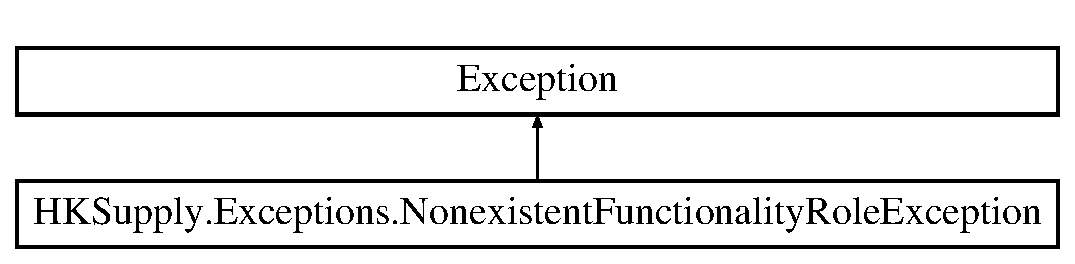
\includegraphics[height=2.000000cm]{class_h_k_supply_1_1_exceptions_1_1_nonexistent_functionality_role_exception}
\end{center}
\end{figure}
\subsection*{Public Member Functions}
\begin{DoxyCompactItemize}
\item 
\mbox{\Hypertarget{class_h_k_supply_1_1_exceptions_1_1_nonexistent_functionality_role_exception_a18ae6c3bbed13d776fbb7407c8c0f839}\label{class_h_k_supply_1_1_exceptions_1_1_nonexistent_functionality_role_exception_a18ae6c3bbed13d776fbb7407c8c0f839}} 
{\bfseries Nonexistent\+Functionality\+Role\+Exception} (string message)
\item 
\mbox{\Hypertarget{class_h_k_supply_1_1_exceptions_1_1_nonexistent_functionality_role_exception_a67c9cb11b716effbea92f6daf598e28f}\label{class_h_k_supply_1_1_exceptions_1_1_nonexistent_functionality_role_exception_a67c9cb11b716effbea92f6daf598e28f}} 
{\bfseries Nonexistent\+Functionality\+Role\+Exception} (string message, System.\+Exception inner)
\end{DoxyCompactItemize}
\subsection*{Protected Member Functions}
\begin{DoxyCompactItemize}
\item 
\mbox{\Hypertarget{class_h_k_supply_1_1_exceptions_1_1_nonexistent_functionality_role_exception_a1c0eef709cc0b2418bc628dfd1199dd1}\label{class_h_k_supply_1_1_exceptions_1_1_nonexistent_functionality_role_exception_a1c0eef709cc0b2418bc628dfd1199dd1}} 
{\bfseries Nonexistent\+Functionality\+Role\+Exception} (System.\+Runtime.\+Serialization.\+Serialization\+Info info, System.\+Runtime.\+Serialization.\+Streaming\+Context context)
\end{DoxyCompactItemize}


\subsection{Detailed Description}
Custom Exception\+: funcionalidad-\/role no existente en el sistema 



The documentation for this class was generated from the following file\+:\begin{DoxyCompactItemize}
\item 
H\+K\+Supply/\+Exceptions/Nonexistent\+Functionality\+Role\+Exception.\+cs\end{DoxyCompactItemize}

\hypertarget{class_h_k_supply_1_1_exceptions_1_1_nonexistent_role_exception}{}\section{H\+K\+Supply.\+Exceptions.\+Nonexistent\+Role\+Exception Class Reference}
\label{class_h_k_supply_1_1_exceptions_1_1_nonexistent_role_exception}\index{H\+K\+Supply.\+Exceptions.\+Nonexistent\+Role\+Exception@{H\+K\+Supply.\+Exceptions.\+Nonexistent\+Role\+Exception}}


Custom Exception\+: Role no existente en el sistema  


Inheritance diagram for H\+K\+Supply.\+Exceptions.\+Nonexistent\+Role\+Exception\+:\begin{figure}[H]
\begin{center}
\leavevmode
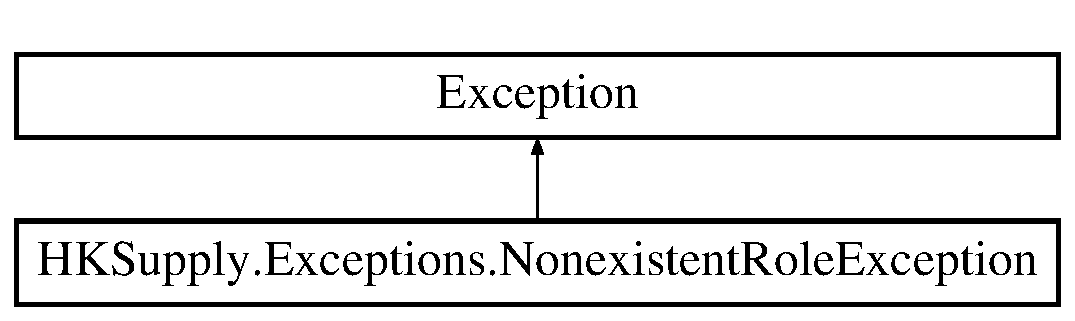
\includegraphics[height=2.000000cm]{class_h_k_supply_1_1_exceptions_1_1_nonexistent_role_exception}
\end{center}
\end{figure}
\subsection*{Public Member Functions}
\begin{DoxyCompactItemize}
\item 
\mbox{\Hypertarget{class_h_k_supply_1_1_exceptions_1_1_nonexistent_role_exception_ad6df76d8577e9e36a22d4e320164ad67}\label{class_h_k_supply_1_1_exceptions_1_1_nonexistent_role_exception_ad6df76d8577e9e36a22d4e320164ad67}} 
{\bfseries Nonexistent\+Role\+Exception} (string message)
\item 
\mbox{\Hypertarget{class_h_k_supply_1_1_exceptions_1_1_nonexistent_role_exception_a052f5db9c0a3c96f399ca79b85f4d6c4}\label{class_h_k_supply_1_1_exceptions_1_1_nonexistent_role_exception_a052f5db9c0a3c96f399ca79b85f4d6c4}} 
{\bfseries Nonexistent\+Role\+Exception} (string message, System.\+Exception inner)
\end{DoxyCompactItemize}
\subsection*{Protected Member Functions}
\begin{DoxyCompactItemize}
\item 
\mbox{\Hypertarget{class_h_k_supply_1_1_exceptions_1_1_nonexistent_role_exception_a27e00d104dc6cbafcf96df82e6f92474}\label{class_h_k_supply_1_1_exceptions_1_1_nonexistent_role_exception_a27e00d104dc6cbafcf96df82e6f92474}} 
{\bfseries Nonexistent\+Role\+Exception} (System.\+Runtime.\+Serialization.\+Serialization\+Info info, System.\+Runtime.\+Serialization.\+Streaming\+Context context)
\end{DoxyCompactItemize}


\subsection{Detailed Description}
Custom Exception\+: Role no existente en el sistema 



The documentation for this class was generated from the following file\+:\begin{DoxyCompactItemize}
\item 
H\+K\+Supply/\+Exceptions/Nonexistent\+Role\+Exception.\+cs\end{DoxyCompactItemize}

\hypertarget{class_h_k_supply_1_1_exceptions_1_1_nonexistent_user_exception}{}\section{H\+K\+Supply.\+Exceptions.\+Nonexistent\+User\+Exception Class Reference}
\label{class_h_k_supply_1_1_exceptions_1_1_nonexistent_user_exception}\index{H\+K\+Supply.\+Exceptions.\+Nonexistent\+User\+Exception@{H\+K\+Supply.\+Exceptions.\+Nonexistent\+User\+Exception}}


Custom Exception\+: Usuario no existente en el sistema  


Inheritance diagram for H\+K\+Supply.\+Exceptions.\+Nonexistent\+User\+Exception\+:\begin{figure}[H]
\begin{center}
\leavevmode
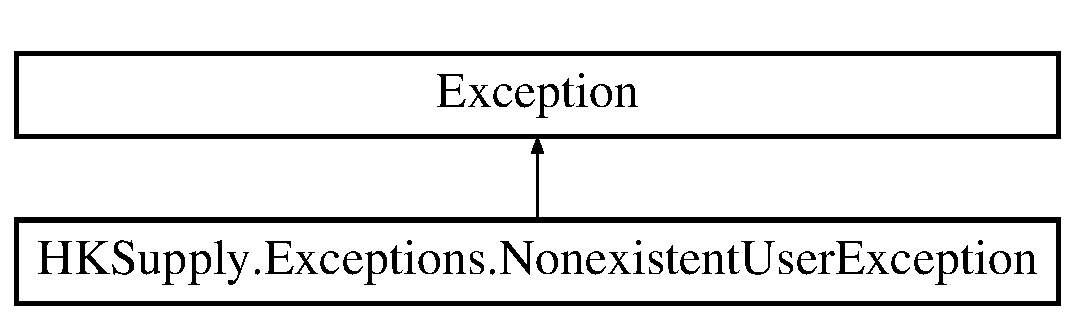
\includegraphics[height=2.000000cm]{class_h_k_supply_1_1_exceptions_1_1_nonexistent_user_exception}
\end{center}
\end{figure}
\subsection*{Public Member Functions}
\begin{DoxyCompactItemize}
\item 
\mbox{\Hypertarget{class_h_k_supply_1_1_exceptions_1_1_nonexistent_user_exception_af1065c421ce7b33b35099c62f271835b}\label{class_h_k_supply_1_1_exceptions_1_1_nonexistent_user_exception_af1065c421ce7b33b35099c62f271835b}} 
{\bfseries Nonexistent\+User\+Exception} (string message)
\item 
\mbox{\Hypertarget{class_h_k_supply_1_1_exceptions_1_1_nonexistent_user_exception_a9d9fd303806bc5c901c13b1ef20bebcb}\label{class_h_k_supply_1_1_exceptions_1_1_nonexistent_user_exception_a9d9fd303806bc5c901c13b1ef20bebcb}} 
{\bfseries Nonexistent\+User\+Exception} (string message, System.\+Exception inner)
\end{DoxyCompactItemize}
\subsection*{Protected Member Functions}
\begin{DoxyCompactItemize}
\item 
\mbox{\Hypertarget{class_h_k_supply_1_1_exceptions_1_1_nonexistent_user_exception_a0545e8560fe9bfdf9fb67c0ed5c04b83}\label{class_h_k_supply_1_1_exceptions_1_1_nonexistent_user_exception_a0545e8560fe9bfdf9fb67c0ed5c04b83}} 
{\bfseries Nonexistent\+User\+Exception} (System.\+Runtime.\+Serialization.\+Serialization\+Info info, System.\+Runtime.\+Serialization.\+Streaming\+Context context)
\end{DoxyCompactItemize}


\subsection{Detailed Description}
Custom Exception\+: Usuario no existente en el sistema 



The documentation for this class was generated from the following file\+:\begin{DoxyCompactItemize}
\item 
H\+K\+Supply/\+Exceptions/Nonexistent\+User\+Exception.\+cs\end{DoxyCompactItemize}

\hypertarget{class_h_k_supply_1_1_migrations_1_1_object_version}{}\section{H\+K\+Supply.\+Migrations.\+Object\+Version Class Reference}
\label{class_h_k_supply_1_1_migrations_1_1_object_version}\index{H\+K\+Supply.\+Migrations.\+Object\+Version@{H\+K\+Supply.\+Migrations.\+Object\+Version}}
Inheritance diagram for H\+K\+Supply.\+Migrations.\+Object\+Version\+:\begin{figure}[H]
\begin{center}
\leavevmode
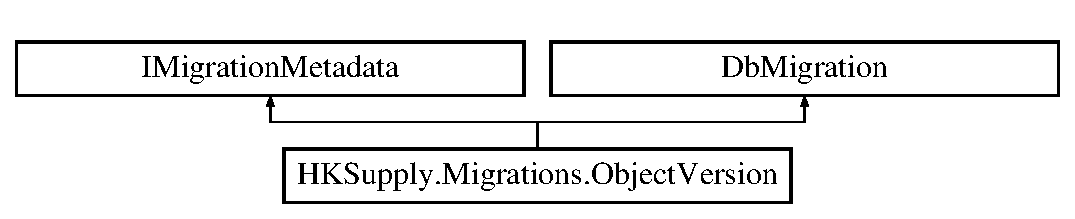
\includegraphics[height=2.000000cm]{class_h_k_supply_1_1_migrations_1_1_object_version}
\end{center}
\end{figure}
\subsection*{Public Member Functions}
\begin{DoxyCompactItemize}
\item 
\mbox{\Hypertarget{class_h_k_supply_1_1_migrations_1_1_object_version_a449ceb0bcf1543c45bc91b37a343210e}\label{class_h_k_supply_1_1_migrations_1_1_object_version_a449ceb0bcf1543c45bc91b37a343210e}} 
override void {\bfseries Up} ()
\item 
\mbox{\Hypertarget{class_h_k_supply_1_1_migrations_1_1_object_version_a08aaee0035439e6c97791a8e9c50a818}\label{class_h_k_supply_1_1_migrations_1_1_object_version_a08aaee0035439e6c97791a8e9c50a818}} 
override void {\bfseries Down} ()
\end{DoxyCompactItemize}


The documentation for this class was generated from the following files\+:\begin{DoxyCompactItemize}
\item 
H\+K\+Supply/\+Migrations/201703081123445\+\_\+\+Object\+Version.\+cs\item 
H\+K\+Supply/\+Migrations/201703081123445\+\_\+\+Object\+Version.\+Designer.\+cs\end{DoxyCompactItemize}

\hypertarget{class_h_k_supply_1_1_migrations_1_1_object_version__2}{}\section{H\+K\+Supply.\+Migrations.\+Object\+Version\+\_\+2 Class Reference}
\label{class_h_k_supply_1_1_migrations_1_1_object_version__2}\index{H\+K\+Supply.\+Migrations.\+Object\+Version\+\_\+2@{H\+K\+Supply.\+Migrations.\+Object\+Version\+\_\+2}}
Inheritance diagram for H\+K\+Supply.\+Migrations.\+Object\+Version\+\_\+2\+:\begin{figure}[H]
\begin{center}
\leavevmode
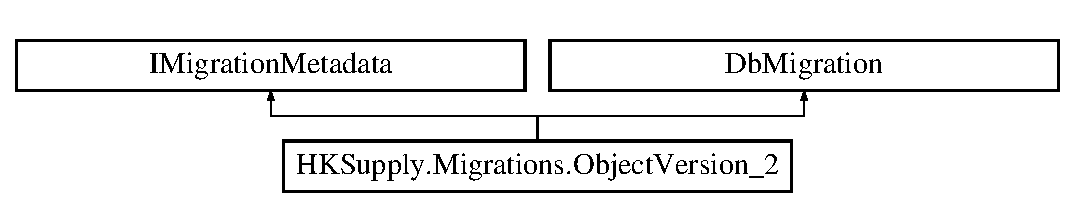
\includegraphics[height=2.000000cm]{class_h_k_supply_1_1_migrations_1_1_object_version__2}
\end{center}
\end{figure}
\subsection*{Public Member Functions}
\begin{DoxyCompactItemize}
\item 
\mbox{\Hypertarget{class_h_k_supply_1_1_migrations_1_1_object_version__2_a3cfd619c6809aa44c8f6ad32cfe652c8}\label{class_h_k_supply_1_1_migrations_1_1_object_version__2_a3cfd619c6809aa44c8f6ad32cfe652c8}} 
override void {\bfseries Up} ()
\item 
\mbox{\Hypertarget{class_h_k_supply_1_1_migrations_1_1_object_version__2_a55a4dc5c3c85c49aba48c2fcf265f5d3}\label{class_h_k_supply_1_1_migrations_1_1_object_version__2_a55a4dc5c3c85c49aba48c2fcf265f5d3}} 
override void {\bfseries Down} ()
\end{DoxyCompactItemize}


The documentation for this class was generated from the following files\+:\begin{DoxyCompactItemize}
\item 
H\+K\+Supply/\+Migrations/201703081126231\+\_\+\+Object\+Version\+\_\+2.\+cs\item 
H\+K\+Supply/\+Migrations/201703081126231\+\_\+\+Object\+Version\+\_\+2.\+Designer.\+cs\end{DoxyCompactItemize}

\hypertarget{class_h_k_supply_1_1_helpers_1_1_password_helper}{}\section{H\+K\+Supply.\+Helpers.\+Password\+Helper Class Reference}
\label{class_h_k_supply_1_1_helpers_1_1_password_helper}\index{H\+K\+Supply.\+Helpers.\+Password\+Helper@{H\+K\+Supply.\+Helpers.\+Password\+Helper}}
\subsection*{Static Public Member Functions}
\begin{DoxyCompactItemize}
\item 
\mbox{\Hypertarget{class_h_k_supply_1_1_helpers_1_1_password_helper_aeaf390a6e70bd83cc7eb210d3d07a89d}\label{class_h_k_supply_1_1_helpers_1_1_password_helper_aeaf390a6e70bd83cc7eb210d3d07a89d}} 
static string {\bfseries Get\+Hash} (string plain\+Text, byte\mbox{[}$\,$\mbox{]} salt\+Bytes=null)
\item 
\mbox{\Hypertarget{class_h_k_supply_1_1_helpers_1_1_password_helper_aeb64d915984f589049e1a3fa9eb91042}\label{class_h_k_supply_1_1_helpers_1_1_password_helper_aeb64d915984f589049e1a3fa9eb91042}} 
static bool {\bfseries Validate\+Pass} (string pass, string hash)
\end{DoxyCompactItemize}


The documentation for this class was generated from the following file\+:\begin{DoxyCompactItemize}
\item 
H\+K\+Supply/\+Helpers/Password\+Helper.\+cs\end{DoxyCompactItemize}

\hypertarget{class_h_k_supply_1_1_models_1_1_role}{}\section{H\+K\+Supply.\+Models.\+Role Class Reference}
\label{class_h_k_supply_1_1_models_1_1_role}\index{H\+K\+Supply.\+Models.\+Role@{H\+K\+Supply.\+Models.\+Role}}
\subsection*{Public Member Functions}
\begin{DoxyCompactItemize}
\item 
\mbox{\Hypertarget{class_h_k_supply_1_1_models_1_1_role_a2e757fafcf931439338d7d02aa2db18a}\label{class_h_k_supply_1_1_models_1_1_role_a2e757fafcf931439338d7d02aa2db18a}} 
override bool {\bfseries Equals} (object obj)
\item 
\mbox{\Hypertarget{class_h_k_supply_1_1_models_1_1_role_a9b7a1c7c9b48374df64a6e8b1080877e}\label{class_h_k_supply_1_1_models_1_1_role_a9b7a1c7c9b48374df64a6e8b1080877e}} 
override int {\bfseries Get\+Hash\+Code} ()
\end{DoxyCompactItemize}
\subsection*{Properties}
\begin{DoxyCompactItemize}
\item 
\mbox{\Hypertarget{class_h_k_supply_1_1_models_1_1_role_ad01af6b00ac5b74ab7289ea10222e79c}\label{class_h_k_supply_1_1_models_1_1_role_ad01af6b00ac5b74ab7289ea10222e79c}} 
string {\bfseries Role\+Id}\hspace{0.3cm}{\ttfamily  \mbox{[}get, set\mbox{]}}
\item 
\mbox{\Hypertarget{class_h_k_supply_1_1_models_1_1_role_aa44073fe223057d72f5a478ed48f9c21}\label{class_h_k_supply_1_1_models_1_1_role_aa44073fe223057d72f5a478ed48f9c21}} 
string {\bfseries Description}\hspace{0.3cm}{\ttfamily  \mbox{[}get, set\mbox{]}}
\item 
\mbox{\Hypertarget{class_h_k_supply_1_1_models_1_1_role_ab925a57eeb388f06023a53f39116db1c}\label{class_h_k_supply_1_1_models_1_1_role_ab925a57eeb388f06023a53f39116db1c}} 
bool {\bfseries Enabled}\hspace{0.3cm}{\ttfamily  \mbox{[}get, set\mbox{]}}
\item 
\mbox{\Hypertarget{class_h_k_supply_1_1_models_1_1_role_a6a9c5c8439262eb82222f80c52e2c0b9}\label{class_h_k_supply_1_1_models_1_1_role_a6a9c5c8439262eb82222f80c52e2c0b9}} 
string {\bfseries Remarks}\hspace{0.3cm}{\ttfamily  \mbox{[}get, set\mbox{]}}
\end{DoxyCompactItemize}


The documentation for this class was generated from the following file\+:\begin{DoxyCompactItemize}
\item 
H\+K\+Supply/\+Models/Role.\+cs\end{DoxyCompactItemize}

\hypertarget{class_h_k_supply_1_1_forms_1_1_master_1_1_role_management}{}\section{H\+K\+Supply.\+Forms.\+Master.\+Role\+Management Class Reference}
\label{class_h_k_supply_1_1_forms_1_1_master_1_1_role_management}\index{H\+K\+Supply.\+Forms.\+Master.\+Role\+Management@{H\+K\+Supply.\+Forms.\+Master.\+Role\+Management}}
Inheritance diagram for H\+K\+Supply.\+Forms.\+Master.\+Role\+Management\+:\begin{figure}[H]
\begin{center}
\leavevmode
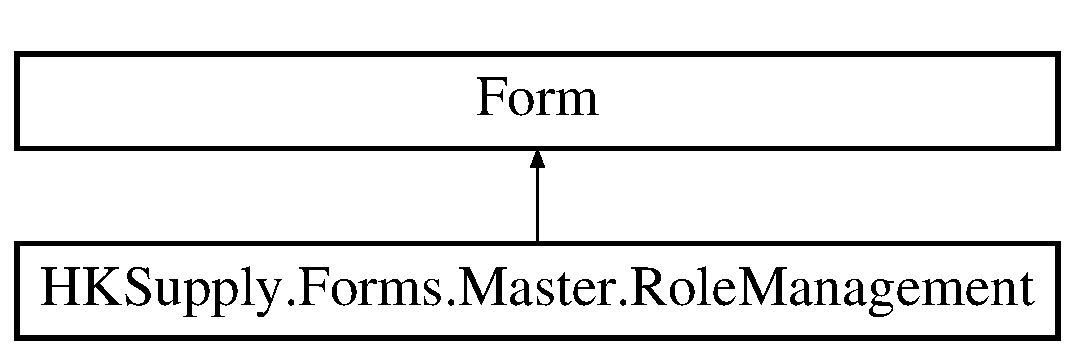
\includegraphics[height=2.000000cm]{class_h_k_supply_1_1_forms_1_1_master_1_1_role_management}
\end{center}
\end{figure}
\subsection*{Public Member Functions}
\begin{DoxyCompactItemize}
\item 
\mbox{\Hypertarget{class_h_k_supply_1_1_forms_1_1_master_1_1_role_management_a029527589b55752c810c410fb7b7ec73}\label{class_h_k_supply_1_1_forms_1_1_master_1_1_role_management_a029527589b55752c810c410fb7b7ec73}} 
void {\bfseries actions\+Stack\+View\+\_\+\+Edit\+Button\+Click} (object sender, Event\+Args e)
\item 
\mbox{\Hypertarget{class_h_k_supply_1_1_forms_1_1_master_1_1_role_management_a9cee7b3dda5de12cd3612ad66b27e302}\label{class_h_k_supply_1_1_forms_1_1_master_1_1_role_management_a9cee7b3dda5de12cd3612ad66b27e302}} 
void {\bfseries actions\+Stack\+View\+\_\+\+New\+Button\+Click} (object sender, Event\+Args e)
\item 
\mbox{\Hypertarget{class_h_k_supply_1_1_forms_1_1_master_1_1_role_management_a6f9ce17d9dbd5e01886e7ffebb428cac}\label{class_h_k_supply_1_1_forms_1_1_master_1_1_role_management_a6f9ce17d9dbd5e01886e7ffebb428cac}} 
void {\bfseries actions\+Stack\+View\+\_\+\+Save\+Button\+Click} (object sender, Event\+Args e)
\item 
\mbox{\Hypertarget{class_h_k_supply_1_1_forms_1_1_master_1_1_role_management_a9651949eef33db6a0600a919bb30f8e8}\label{class_h_k_supply_1_1_forms_1_1_master_1_1_role_management_a9651949eef33db6a0600a919bb30f8e8}} 
void {\bfseries actions\+Stack\+View\+\_\+\+Cancel\+Button\+Click} (object sender, Event\+Args e)
\item 
\mbox{\Hypertarget{class_h_k_supply_1_1_forms_1_1_master_1_1_role_management_a022e071b082ef46f206426f75db34fa8}\label{class_h_k_supply_1_1_forms_1_1_master_1_1_role_management_a022e071b082ef46f206426f75db34fa8}} 
void {\bfseries Configure\+Actions\+Stack\+View} ()
\end{DoxyCompactItemize}
\subsection*{Protected Member Functions}
\begin{DoxyCompactItemize}
\item 
override void \hyperlink{class_h_k_supply_1_1_forms_1_1_master_1_1_role_management_aec6f44de37a82c49e6166b2d83e65885}{Dispose} (bool disposing)
\begin{DoxyCompactList}\small\item\em Clean up any resources being used. \end{DoxyCompactList}\end{DoxyCompactItemize}


\subsection{Member Function Documentation}
\mbox{\Hypertarget{class_h_k_supply_1_1_forms_1_1_master_1_1_role_management_aec6f44de37a82c49e6166b2d83e65885}\label{class_h_k_supply_1_1_forms_1_1_master_1_1_role_management_aec6f44de37a82c49e6166b2d83e65885}} 
\index{H\+K\+Supply\+::\+Forms\+::\+Master\+::\+Role\+Management@{H\+K\+Supply\+::\+Forms\+::\+Master\+::\+Role\+Management}!Dispose@{Dispose}}
\index{Dispose@{Dispose}!H\+K\+Supply\+::\+Forms\+::\+Master\+::\+Role\+Management@{H\+K\+Supply\+::\+Forms\+::\+Master\+::\+Role\+Management}}
\subsubsection{\texorpdfstring{Dispose()}{Dispose()}}
{\footnotesize\ttfamily override void H\+K\+Supply.\+Forms.\+Master.\+Role\+Management.\+Dispose (\begin{DoxyParamCaption}\item[{bool}]{disposing }\end{DoxyParamCaption})\hspace{0.3cm}{\ttfamily [protected]}}



Clean up any resources being used. 


\begin{DoxyParams}{Parameters}
{\em disposing} & true if managed resources should be disposed; otherwise, false.\\
\hline
\end{DoxyParams}


The documentation for this class was generated from the following files\+:\begin{DoxyCompactItemize}
\item 
H\+K\+Supply/\+Forms/\+Master/Role\+Management.\+cs\item 
H\+K\+Supply/\+Forms/\+Master/Role\+Management.\+Designer.\+cs\end{DoxyCompactItemize}

\hypertarget{class_h_k_suply_1_1_unit_test_1_1_role_test}{}\section{H\+K\+Suply.\+Unit\+Test.\+Role\+Test Class Reference}
\label{class_h_k_suply_1_1_unit_test_1_1_role_test}\index{H\+K\+Suply.\+Unit\+Test.\+Role\+Test@{H\+K\+Suply.\+Unit\+Test.\+Role\+Test}}
\subsection*{Public Member Functions}
\begin{DoxyCompactItemize}
\item 
\mbox{\Hypertarget{class_h_k_suply_1_1_unit_test_1_1_role_test_aa9d71210dc474e284fe04b9bd38a122b}\label{class_h_k_suply_1_1_unit_test_1_1_role_test_aa9d71210dc474e284fe04b9bd38a122b}} 
void {\bfseries Get\+All\+Roles} ()
\item 
\mbox{\Hypertarget{class_h_k_suply_1_1_unit_test_1_1_role_test_a8a280b4286b4071e13440d7c7f179e13}\label{class_h_k_suply_1_1_unit_test_1_1_role_test_a8a280b4286b4071e13440d7c7f179e13}} 
void {\bfseries Get\+Role} ()
\item 
\mbox{\Hypertarget{class_h_k_suply_1_1_unit_test_1_1_role_test_ad7e762c47c24c111dac35a0539f1325a}\label{class_h_k_suply_1_1_unit_test_1_1_role_test_ad7e762c47c24c111dac35a0539f1325a}} 
void {\bfseries New\+Role} ()
\item 
\mbox{\Hypertarget{class_h_k_suply_1_1_unit_test_1_1_role_test_ad1920b59b54f4b79a8aefb62060d6375}\label{class_h_k_suply_1_1_unit_test_1_1_role_test_ad1920b59b54f4b79a8aefb62060d6375}} 
void {\bfseries Disable\+Role} ()
\item 
\mbox{\Hypertarget{class_h_k_suply_1_1_unit_test_1_1_role_test_a515e4f6d1342bc184a49a94d6d97835d}\label{class_h_k_suply_1_1_unit_test_1_1_role_test_a515e4f6d1342bc184a49a94d6d97835d}} 
void {\bfseries Update\+Roles} ()
\end{DoxyCompactItemize}


The documentation for this class was generated from the following file\+:\begin{DoxyCompactItemize}
\item 
H\+K\+Suply.\+Unit\+Test/Role\+Test.\+cs\end{DoxyCompactItemize}

\hypertarget{class_custom_controls_1_1_stack_view}{}\section{Custom\+Controls.\+Stack\+View Class Reference}
\label{class_custom_controls_1_1_stack_view}\index{Custom\+Controls.\+Stack\+View@{Custom\+Controls.\+Stack\+View}}
Inheritance diagram for Custom\+Controls.\+Stack\+View\+:\begin{figure}[H]
\begin{center}
\leavevmode
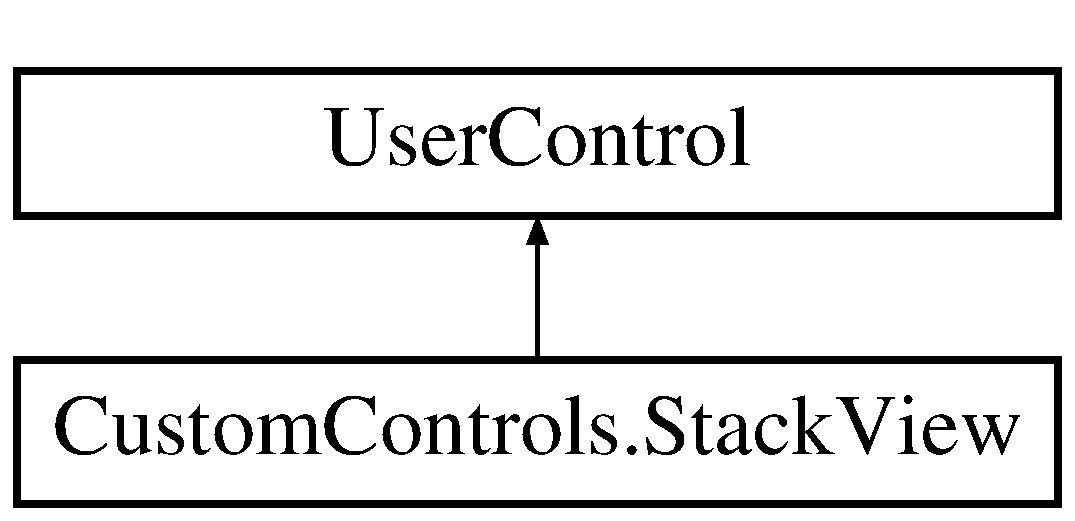
\includegraphics[height=2.000000cm]{class_custom_controls_1_1_stack_view}
\end{center}
\end{figure}
\subsection*{Public Types}
\begin{DoxyCompactItemize}
\item 
\mbox{\Hypertarget{class_custom_controls_1_1_stack_view_ad33a71dff7cc2c25851d7cd5d75fb3c8}\label{class_custom_controls_1_1_stack_view_ad33a71dff7cc2c25851d7cd5d75fb3c8}} 
enum {\bfseries Toolbar\+States} \{ \newline
{\bfseries Only\+Read}, 
{\bfseries Only\+Edit}, 
{\bfseries Only\+Edit\+New}, 
{\bfseries Edit}, 
\newline
{\bfseries New}
 \}
\end{DoxyCompactItemize}
\subsection*{Public Member Functions}
\begin{DoxyCompactItemize}
\item 
\mbox{\Hypertarget{class_custom_controls_1_1_stack_view_af1226e4d40a4f58799de5b48de95c275}\label{class_custom_controls_1_1_stack_view_af1226e4d40a4f58799de5b48de95c275}} 
{\bfseries Stack\+View} (bool read, bool create, bool modify)
\item 
\mbox{\Hypertarget{class_custom_controls_1_1_stack_view_a40e9b83536de3aa4a3fd7e40bfce0246}\label{class_custom_controls_1_1_stack_view_a40e9b83536de3aa4a3fd7e40bfce0246}} 
void {\bfseries Initialize\+General\+Style} ()
\item 
\mbox{\Hypertarget{class_custom_controls_1_1_stack_view_aa6ee6db47352fbb47bc1292ea7f58611}\label{class_custom_controls_1_1_stack_view_aa6ee6db47352fbb47bc1292ea7f58611}} 
void {\bfseries Restore\+Init\+State} ()
\end{DoxyCompactItemize}
\subsection*{Protected Member Functions}
\begin{DoxyCompactItemize}
\item 
\mbox{\Hypertarget{class_custom_controls_1_1_stack_view_a19b739e8edd30f174bfe870081ecfed3}\label{class_custom_controls_1_1_stack_view_a19b739e8edd30f174bfe870081ecfed3}} 
virtual void {\bfseries On\+Edit\+Button\+Click} (Event\+Args e)
\item 
\mbox{\Hypertarget{class_custom_controls_1_1_stack_view_a11ce82dee60bdffc83f7d3ebdf10b17a}\label{class_custom_controls_1_1_stack_view_a11ce82dee60bdffc83f7d3ebdf10b17a}} 
virtual void {\bfseries On\+New\+Button\+Click} (Event\+Args e)
\item 
\mbox{\Hypertarget{class_custom_controls_1_1_stack_view_a77a46c2d55bf40ed18bcfe90dcaf3805}\label{class_custom_controls_1_1_stack_view_a77a46c2d55bf40ed18bcfe90dcaf3805}} 
virtual void {\bfseries On\+Save\+Button\+Click} (Event\+Args e)
\item 
\mbox{\Hypertarget{class_custom_controls_1_1_stack_view_a48997386c95398640506e1e5ada5f0dd}\label{class_custom_controls_1_1_stack_view_a48997386c95398640506e1e5ada5f0dd}} 
virtual void {\bfseries On\+Cancel\+Button\+Click} (Event\+Args e)
\item 
override void \hyperlink{class_custom_controls_1_1_stack_view_a227a09aebaaa2cc577a4bfa50cb08967}{Dispose} (bool disposing)
\begin{DoxyCompactList}\small\item\em Limpiar los recursos que se estén utilizando. \end{DoxyCompactList}\end{DoxyCompactItemize}
\subsection*{Properties}
\begin{DoxyCompactItemize}
\item 
\mbox{\Hypertarget{class_custom_controls_1_1_stack_view_a71200adab4464290b2df815e233b5bf9}\label{class_custom_controls_1_1_stack_view_a71200adab4464290b2df815e233b5bf9}} 
Toolbar\+States {\bfseries Current\+State}\hspace{0.3cm}{\ttfamily  \mbox{[}get\mbox{]}}
\end{DoxyCompactItemize}
\subsection*{Events}
\begin{DoxyCompactItemize}
\item 
\mbox{\Hypertarget{class_custom_controls_1_1_stack_view_a63d3aaa67d3d681a55e44abfdc1e18a8}\label{class_custom_controls_1_1_stack_view_a63d3aaa67d3d681a55e44abfdc1e18a8}} 
Event\+Handler {\bfseries Edit\+Button\+Click}
\item 
\mbox{\Hypertarget{class_custom_controls_1_1_stack_view_af19003ef6d5198e763c656b624c3fbbc}\label{class_custom_controls_1_1_stack_view_af19003ef6d5198e763c656b624c3fbbc}} 
Event\+Handler {\bfseries New\+Button\+Click}
\item 
\mbox{\Hypertarget{class_custom_controls_1_1_stack_view_a6086b716160faebc479c3a407092a7d5}\label{class_custom_controls_1_1_stack_view_a6086b716160faebc479c3a407092a7d5}} 
Event\+Handler {\bfseries Save\+Button\+Click}
\item 
\mbox{\Hypertarget{class_custom_controls_1_1_stack_view_a19d78699d1abcd1c49f4941b58f76800}\label{class_custom_controls_1_1_stack_view_a19d78699d1abcd1c49f4941b58f76800}} 
Event\+Handler {\bfseries Cancel\+Button\+Click}
\end{DoxyCompactItemize}


\subsection{Member Function Documentation}
\mbox{\Hypertarget{class_custom_controls_1_1_stack_view_a227a09aebaaa2cc577a4bfa50cb08967}\label{class_custom_controls_1_1_stack_view_a227a09aebaaa2cc577a4bfa50cb08967}} 
\index{Custom\+Controls\+::\+Stack\+View@{Custom\+Controls\+::\+Stack\+View}!Dispose@{Dispose}}
\index{Dispose@{Dispose}!Custom\+Controls\+::\+Stack\+View@{Custom\+Controls\+::\+Stack\+View}}
\subsubsection{\texorpdfstring{Dispose()}{Dispose()}}
{\footnotesize\ttfamily override void Custom\+Controls.\+Stack\+View.\+Dispose (\begin{DoxyParamCaption}\item[{bool}]{disposing }\end{DoxyParamCaption})\hspace{0.3cm}{\ttfamily [protected]}}



Limpiar los recursos que se estén utilizando. 


\begin{DoxyParams}{Parameters}
{\em disposing} & true si los recursos administrados se deben eliminar; false en caso contrario.\\
\hline
\end{DoxyParams}


The documentation for this class was generated from the following files\+:\begin{DoxyCompactItemize}
\item 
Custom\+Controls/Stack\+View.\+cs\item 
Custom\+Controls/Stack\+View.\+Designer.\+cs\end{DoxyCompactItemize}

\hypertarget{class_unit_test_project_1_1_unit_test1}{}\section{Unit\+Test\+Project.\+Unit\+Test1 Class Reference}
\label{class_unit_test_project_1_1_unit_test1}\index{Unit\+Test\+Project.\+Unit\+Test1@{Unit\+Test\+Project.\+Unit\+Test1}}
\subsection*{Public Member Functions}
\begin{DoxyCompactItemize}
\item 
\mbox{\Hypertarget{class_unit_test_project_1_1_unit_test1_a1cd53bf019a6a5ac0422147c8b1434da}\label{class_unit_test_project_1_1_unit_test1_a1cd53bf019a6a5ac0422147c8b1434da}} 
void {\bfseries Test\+Method1} ()
\end{DoxyCompactItemize}


The documentation for this class was generated from the following file\+:\begin{DoxyCompactItemize}
\item 
Unit\+Test\+Project/Unit\+Test1.\+cs\end{DoxyCompactItemize}

\hypertarget{class_h_k_supply_1_1_models_1_1_user}{}\section{H\+K\+Supply.\+Models.\+User Class Reference}
\label{class_h_k_supply_1_1_models_1_1_user}\index{H\+K\+Supply.\+Models.\+User@{H\+K\+Supply.\+Models.\+User}}
\subsection*{Public Member Functions}
\begin{DoxyCompactItemize}
\item 
\mbox{\Hypertarget{class_h_k_supply_1_1_models_1_1_user_a24e2282b6384346f60d42ae98dfc849f}\label{class_h_k_supply_1_1_models_1_1_user_a24e2282b6384346f60d42ae98dfc849f}} 
override bool {\bfseries Equals} (object obj)
\item 
\mbox{\Hypertarget{class_h_k_supply_1_1_models_1_1_user_a79d46e0361441e50d049d6b729db4906}\label{class_h_k_supply_1_1_models_1_1_user_a79d46e0361441e50d049d6b729db4906}} 
override int {\bfseries Get\+Hash\+Code} ()
\end{DoxyCompactItemize}
\subsection*{Properties}
\begin{DoxyCompactItemize}
\item 
\mbox{\Hypertarget{class_h_k_supply_1_1_models_1_1_user_a02e00589ab7bb27c4173f7855e0e8050}\label{class_h_k_supply_1_1_models_1_1_user_a02e00589ab7bb27c4173f7855e0e8050}} 
int {\bfseries Id}\hspace{0.3cm}{\ttfamily  \mbox{[}get, set\mbox{]}}
\item 
\mbox{\Hypertarget{class_h_k_supply_1_1_models_1_1_user_ae40491b88829110d5840f205f046bbc1}\label{class_h_k_supply_1_1_models_1_1_user_ae40491b88829110d5840f205f046bbc1}} 
string {\bfseries User\+Login}\hspace{0.3cm}{\ttfamily  \mbox{[}get, set\mbox{]}}
\item 
\mbox{\Hypertarget{class_h_k_supply_1_1_models_1_1_user_a3f8a8a968733495182ed49af9170f613}\label{class_h_k_supply_1_1_models_1_1_user_a3f8a8a968733495182ed49af9170f613}} 
string {\bfseries Password}\hspace{0.3cm}{\ttfamily  \mbox{[}get, set\mbox{]}}
\item 
\mbox{\Hypertarget{class_h_k_supply_1_1_models_1_1_user_ac7284de399f20c1ed232caae7c20620e}\label{class_h_k_supply_1_1_models_1_1_user_ac7284de399f20c1ed232caae7c20620e}} 
string {\bfseries Name}\hspace{0.3cm}{\ttfamily  \mbox{[}get, set\mbox{]}}
\item 
\mbox{\Hypertarget{class_h_k_supply_1_1_models_1_1_user_a7bde19a172a7c4942b1f9ad7307d6722}\label{class_h_k_supply_1_1_models_1_1_user_a7bde19a172a7c4942b1f9ad7307d6722}} 
string {\bfseries Role\+Id}\hspace{0.3cm}{\ttfamily  \mbox{[}get, set\mbox{]}}
\item 
\mbox{\Hypertarget{class_h_k_supply_1_1_models_1_1_user_aa0733f43797c5f8b6bd91e23a2613b90}\label{class_h_k_supply_1_1_models_1_1_user_aa0733f43797c5f8b6bd91e23a2613b90}} 
\mbox{\hyperlink{class_h_k_supply_1_1_models_1_1_role}{Role}} {\bfseries User\+Role}\hspace{0.3cm}{\ttfamily  \mbox{[}get, set\mbox{]}}
\item 
\mbox{\Hypertarget{class_h_k_supply_1_1_models_1_1_user_ac2fb577af717342e21a9ac4d49283477}\label{class_h_k_supply_1_1_models_1_1_user_ac2fb577af717342e21a9ac4d49283477}} 
bool {\bfseries Enabled}\hspace{0.3cm}{\ttfamily  \mbox{[}get, set\mbox{]}}
\item 
\mbox{\Hypertarget{class_h_k_supply_1_1_models_1_1_user_ad73610de042dfdb05a48503dab3c43b4}\label{class_h_k_supply_1_1_models_1_1_user_ad73610de042dfdb05a48503dab3c43b4}} 
Date\+Time {\bfseries Last\+Login}\hspace{0.3cm}{\ttfamily  \mbox{[}get, set\mbox{]}}
\item 
\mbox{\Hypertarget{class_h_k_supply_1_1_models_1_1_user_a8b7622cd2a564e0c11ae2ea3eb7fdadc}\label{class_h_k_supply_1_1_models_1_1_user_a8b7622cd2a564e0c11ae2ea3eb7fdadc}} 
Date\+Time {\bfseries Last\+Logout}\hspace{0.3cm}{\ttfamily  \mbox{[}get, set\mbox{]}}
\item 
\mbox{\Hypertarget{class_h_k_supply_1_1_models_1_1_user_a147c1d1d721f15b477caaf2b6ce75321}\label{class_h_k_supply_1_1_models_1_1_user_a147c1d1d721f15b477caaf2b6ce75321}} 
string {\bfseries Remarks}\hspace{0.3cm}{\ttfamily  \mbox{[}get, set\mbox{]}}
\end{DoxyCompactItemize}


The documentation for this class was generated from the following file\+:\begin{DoxyCompactItemize}
\item 
H\+K\+Supply/\+Models/User.\+cs\end{DoxyCompactItemize}

\hypertarget{class_h_k_supply_1_1_forms_1_1_master_1_1_user_management}{}\section{H\+K\+Supply.\+Forms.\+Master.\+User\+Management Class Reference}
\label{class_h_k_supply_1_1_forms_1_1_master_1_1_user_management}\index{H\+K\+Supply.\+Forms.\+Master.\+User\+Management@{H\+K\+Supply.\+Forms.\+Master.\+User\+Management}}
Inheritance diagram for H\+K\+Supply.\+Forms.\+Master.\+User\+Management\+:\begin{figure}[H]
\begin{center}
\leavevmode
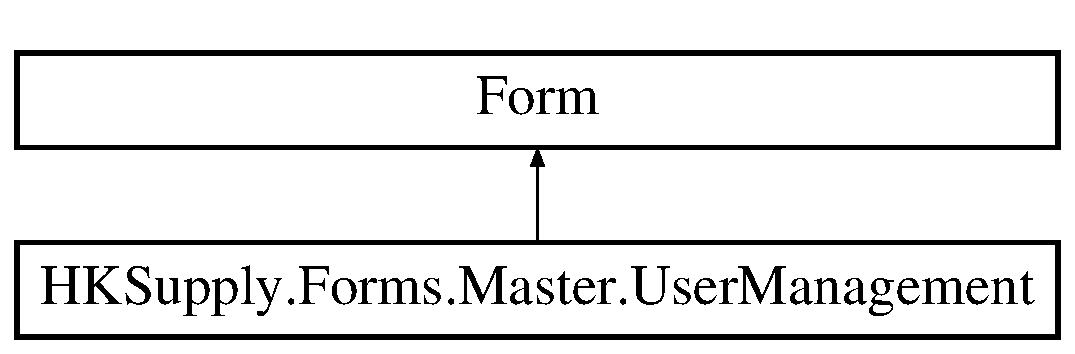
\includegraphics[height=3.000000cm]{class_h_k_supply_1_1_forms_1_1_master_1_1_user_management}
\end{center}
\end{figure}
\subsection*{Public Member Functions}
\begin{DoxyCompactItemize}
\item 
\mbox{\Hypertarget{class_h_k_supply_1_1_forms_1_1_master_1_1_user_management_a333537f209a865c88129f6cb731d04c7}\label{class_h_k_supply_1_1_forms_1_1_master_1_1_user_management_a333537f209a865c88129f6cb731d04c7}} 
override void {\bfseries bbi\+Cancel\+\_\+\+Item\+Click} (object sender, Dev\+Express.\+Xtra\+Bars.\+Item\+Click\+Event\+Args e)
\item 
\mbox{\Hypertarget{class_h_k_supply_1_1_forms_1_1_master_1_1_user_management_a42e75f35c50451a97a081cf6c519c4eb}\label{class_h_k_supply_1_1_forms_1_1_master_1_1_user_management_a42e75f35c50451a97a081cf6c519c4eb}} 
override void {\bfseries bbi\+Edit\+\_\+\+Item\+Click} (object sender, Dev\+Express.\+Xtra\+Bars.\+Item\+Click\+Event\+Args e)
\item 
\mbox{\Hypertarget{class_h_k_supply_1_1_forms_1_1_master_1_1_user_management_a336715a44ac9d357a9fb64207d2f0d23}\label{class_h_k_supply_1_1_forms_1_1_master_1_1_user_management_a336715a44ac9d357a9fb64207d2f0d23}} 
override void {\bfseries bbi\+New\+\_\+\+Item\+Click} (object sender, Dev\+Express.\+Xtra\+Bars.\+Item\+Click\+Event\+Args e)
\item 
\mbox{\Hypertarget{class_h_k_supply_1_1_forms_1_1_master_1_1_user_management_a691087c2437afe71e0fc1b2760905040}\label{class_h_k_supply_1_1_forms_1_1_master_1_1_user_management_a691087c2437afe71e0fc1b2760905040}} 
override void {\bfseries bbi\+Save\+\_\+\+Item\+Click} (object sender, Dev\+Express.\+Xtra\+Bars.\+Item\+Click\+Event\+Args e)
\end{DoxyCompactItemize}
\subsection*{Protected Member Functions}
\begin{DoxyCompactItemize}
\item 
override void \mbox{\hyperlink{class_h_k_supply_1_1_forms_1_1_master_1_1_user_management_a785e8f8b502b3ac465677f0817b29023}{Dispose}} (bool disposing)
\begin{DoxyCompactList}\small\item\em Clean up any resources being used. \end{DoxyCompactList}\end{DoxyCompactItemize}
\subsection*{Additional Inherited Members}


\subsection{Member Function Documentation}
\mbox{\Hypertarget{class_h_k_supply_1_1_forms_1_1_master_1_1_user_management_a785e8f8b502b3ac465677f0817b29023}\label{class_h_k_supply_1_1_forms_1_1_master_1_1_user_management_a785e8f8b502b3ac465677f0817b29023}} 
\index{H\+K\+Supply\+::\+Forms\+::\+Master\+::\+User\+Management@{H\+K\+Supply\+::\+Forms\+::\+Master\+::\+User\+Management}!Dispose@{Dispose}}
\index{Dispose@{Dispose}!H\+K\+Supply\+::\+Forms\+::\+Master\+::\+User\+Management@{H\+K\+Supply\+::\+Forms\+::\+Master\+::\+User\+Management}}
\subsubsection{\texorpdfstring{Dispose()}{Dispose()}}
{\footnotesize\ttfamily override void H\+K\+Supply.\+Forms.\+Master.\+User\+Management.\+Dispose (\begin{DoxyParamCaption}\item[{bool}]{disposing }\end{DoxyParamCaption})\hspace{0.3cm}{\ttfamily [protected]}}



Clean up any resources being used. 


\begin{DoxyParams}{Parameters}
{\em disposing} & true if managed resources should be disposed; otherwise, false.\\
\hline
\end{DoxyParams}


The documentation for this class was generated from the following files\+:\begin{DoxyCompactItemize}
\item 
H\+K\+Supply/\+Forms/\+Master/User\+Management.\+cs\item 
H\+K\+Supply/\+Forms/\+Master/User\+Management.\+Designer.\+cs\end{DoxyCompactItemize}

\hypertarget{class_h_k_suply_1_1_unit_test_1_1_user_test}{}\section{H\+K\+Suply.\+Unit\+Test.\+User\+Test Class Reference}
\label{class_h_k_suply_1_1_unit_test_1_1_user_test}\index{H\+K\+Suply.\+Unit\+Test.\+User\+Test@{H\+K\+Suply.\+Unit\+Test.\+User\+Test}}
\subsection*{Public Member Functions}
\begin{DoxyCompactItemize}
\item 
\mbox{\Hypertarget{class_h_k_suply_1_1_unit_test_1_1_user_test_a3b155a2e3f798000decc5cd9bb7ff5bc}\label{class_h_k_suply_1_1_unit_test_1_1_user_test_a3b155a2e3f798000decc5cd9bb7ff5bc}} 
void {\bfseries Get\+All\+User} ()
\item 
\mbox{\Hypertarget{class_h_k_suply_1_1_unit_test_1_1_user_test_a0d33d16a2e9761ccdf686fc6398bd599}\label{class_h_k_suply_1_1_unit_test_1_1_user_test_a0d33d16a2e9761ccdf686fc6398bd599}} 
void {\bfseries Get\+User} ()
\item 
\mbox{\Hypertarget{class_h_k_suply_1_1_unit_test_1_1_user_test_a38a60511778b95f7cd2c256697cc4e6f}\label{class_h_k_suply_1_1_unit_test_1_1_user_test_a38a60511778b95f7cd2c256697cc4e6f}} 
void {\bfseries New\+User} ()
\item 
\mbox{\Hypertarget{class_h_k_suply_1_1_unit_test_1_1_user_test_acc37fae05da85affd3a422b32bcd0700}\label{class_h_k_suply_1_1_unit_test_1_1_user_test_acc37fae05da85affd3a422b32bcd0700}} 
void {\bfseries Disable\+User} ()
\item 
\mbox{\Hypertarget{class_h_k_suply_1_1_unit_test_1_1_user_test_ac77e49a4ff678e5325e0634aa8425f09}\label{class_h_k_suply_1_1_unit_test_1_1_user_test_ac77e49a4ff678e5325e0634aa8425f09}} 
void {\bfseries Change\+Password} ()
\item 
\mbox{\Hypertarget{class_h_k_suply_1_1_unit_test_1_1_user_test_a8e2c7128da98aa8edb6541a4c037c56d}\label{class_h_k_suply_1_1_unit_test_1_1_user_test_a8e2c7128da98aa8edb6541a4c037c56d}} 
void {\bfseries Update\+Users} ()
\end{DoxyCompactItemize}


The documentation for this class was generated from the following file\+:\begin{DoxyCompactItemize}
\item 
H\+K\+Suply.\+Unit\+Test/User\+Test.\+cs\end{DoxyCompactItemize}

%--- End generated contents ---

% Index
\backmatter
\newpage
\phantomsection
\clearemptydoublepage
\addcontentsline{toc}{chapter}{Index}
\printindex

\end{document}
